\documentclass[a4paper,11pt,]{book} % draft

\usepackage{silence}
\WarningFilter{fourier}{Please consider}
\WarningFilter{hyperref}{Token not allowed in a PDF string}

\usepackage[T1]{fontenc}
\usepackage{fontspec}
\usepackage[french,english]{babel}
\setmonofont{Ubuntu Mono}
\setlength{\textwidth}{146.8mm}
\setlength{\oddsidemargin}{11.6mm}
\setlength{\evensidemargin}{0.8mm}
\setlength{\topmargin}{-2.2mm}
\setlength{\textheight}{221.9mm}
\setlength{\headheight}{14pt}

\usepackage{setspace}
\setstretch{1.1}
\makeatletter
\setlength{\@fptop}{0pt}
\makeatother

\usepackage{lmodern}
\usepackage{fourier}
\usepackage{graphicx}
\usepackage{xcolor}
\usepackage{booktabs}
\usepackage{lipsum}
\usepackage[final]{microtype}
\usepackage[hyphens]{url}

\usepackage{fancyhdr}
\renewcommand{\sectionmark}[1]{\markright{\thesection\ #1}}
\pagestyle{fancy}
  \fancyhf{}
  \renewcommand{\headrulewidth}{0.4pt}
  \renewcommand{\footrulewidth}{0pt}
  \fancyhead[OR]{\bfseries \nouppercase{\rightmark}}
  \fancyhead[EL]{\bfseries \nouppercase{\leftmark}}
  \fancyfoot[EL,OR]{\thepage}
\fancypagestyle{plain}{
  \fancyhf{}
  \renewcommand{\headrulewidth}{0pt}
  \renewcommand{\footrulewidth}{0pt}
  \fancyfoot[EL,OR]{\thepage}}
\fancypagestyle{addpagenumbersforpdfimports}{
  \fancyhead{}
  \renewcommand{\headrulewidth}{0pt}
  \fancyfoot{}
  \fancyfoot[RO,LE]{\thepage}
}

\usepackage[final]{hyperref}
\definecolor[named]{purplish}{cmyk}{0.55,1,0,0.15}
\definecolor[named]{darkblueish}{cmyk}{1,0.58,0,0.21}
\hypersetup{
  colorlinks=true,
  pdfborder={0 0 0},
  linkcolor=purplish,
  citecolor=purplish,
  urlcolor=darkblueish,
  filecolor=darkblueish}
\urlstyle{same}
\usepackage[final]{pdfpages}
\usepackage{bookmark}

\makeatletter
\renewcommand\@pnumwidth{20pt}
\makeatother

\makeatletter
\def\cleardoublepage{\clearpage\if@twoside \ifodd\c@page\else
    \hbox{}
    \thispagestyle{empty}
    \newpage
    \if@twocolumn\hbox{}\newpage\fi\fi\fi}
\makeatother \clearpage{\pagestyle{plain}\cleardoublepage}

\usepackage{color}
\usepackage{tikz}
\usepackage[explicit]{titlesec}
\newcommand*\chapterlabel{}
\titleformat{\chapter}[display]
  {\normalfont\bfseries\Huge}
  {\gdef\chapterlabel{\thechapter\ }}
  {0pt}
    {\begin{tikzpicture}[remember picture,overlay]
    \node[yshift=-8cm] at (current page.north west)
      {\begin{tikzpicture}[remember picture, overlay]
        \draw[fill=black] (0,0) rectangle(35.5mm,15mm);
        \node[anchor=north east,yshift=-7.2cm,xshift=34mm,minimum height=30mm,inner sep=0mm] at (current page.north west)
        {\parbox[top][30mm][t]{15mm}{\raggedleft \rule{0cm}{0.6cm}\color{white}\chapterlabel}};  %the empty rule is just to get better base-line alignment
        \node[anchor=north west,yshift=-7.2cm,xshift=37mm,text width=\textwidth,minimum height=30mm,inner sep=0mm] at (current page.north west)
              {\parbox[top][30mm][t]{\textwidth}{\rule{0cm}{0.6cm}\color{black}#1}};
       \end{tikzpicture}
      };
   \end{tikzpicture}
   \gdef\chapterlabel{}
  } % code before the title body
\titlespacing*{name=\chapter,numberless}{-3.7cm}{83.2pt-\parskip}{-3.2pt+\parskip}
\titlespacing*{\chapter}{-3.7cm}{50pt-\parskip-\parskip}{30pt+\parskip+\parskip}
\titlespacing*{\section}{0pt}{13.2pt}{1em-\parskip}  % 13.2pt is line spacing for a text with 11pt font size
\titlespacing*{\subsection}{0pt}{13.2pt}{1em-\parskip}
\titlespacing*{\subsubsection}{0pt}{13.2pt}{1em-\parskip}
\titlespacing*{\paragraph}{0pt}{13.2pt}{1em-\parskip}

\newcounter{myparts}
\newcommand*\partlabel{}
\titleformat{\part}[display]  % type (section,chapter,etc...) to vary,  shape (eg display-type)
  {\normalfont\bfseries\Huge} % format of the part
  {\gdef\partlabel{\thepart\ }}     % the label
  {0pt} % separation between label and part-title
    {\ifpdf\setlength{\unitlength}{20mm}\else\setlength{\unitlength}{0mm}\fi
    \addtocounter{myparts}{1}
    \begin{tikzpicture}[remember picture,overlay]
    \node[anchor=north west,xshift=-65mm,yshift=-6.9cm-\value{myparts}*20mm] at (current page.north east) % for unknown reasons: 3mm missing -> 65 instead of 62
      {\begin{tikzpicture}[remember picture, overlay]
        \draw[fill=black] (0,0) rectangle(62mm,20mm);   % -\value{myparts}\unitlength
        \node[anchor=north west,yshift=-6.1cm-\value{myparts}*\unitlength,xshift=-60.5mm,minimum height=30mm,inner sep=0mm] at (current page.north east)
        {\parbox[top][30mm][t]{55mm}{\raggedright \color{white}Part \partlabel \rule{0cm}{0.6cm}}};  %the empty rule is just to get better base-line alignment
        \node[anchor=north east,yshift=-6.1cm-\value{myparts}*\unitlength,xshift=-63.5mm,text width=\textwidth,minimum height=30mm,inner sep=0mm] at (current page.north east)
              {\parbox[top][30mm][t]{\textwidth}{\raggedleft \rule{0cm}{0.6cm}\color{black}#1}};
       \end{tikzpicture}
      };
   \end{tikzpicture}
   \gdef\partlabel{}
  } % code before the title body
\titlespacing*{\part}{11.06cm}{26.4pt-\parskip-\parskip}{0pt}

\usepackage{amsmath}
\usepackage{amsfonts}
\usepackage{amssymb}
\usepackage{mathtools}
\usepackage{xstring}
% Fix the problem with delimiter size caused by fourier and amsmath packages.
\makeatletter
\def\resetMathstrut@{%
  \setbox\z@\hbox{%
    \mathchardef\@tempa\mathcode`\(\relax
      \def\@tempb##1"##2##3{\the\textfont"##3\char"}%
      \expandafter\@tempb\meaning\@tempa \relax
  }%
  \ht\Mathstrutbox@1.2\ht\z@ \dp\Mathstrutbox@1.2\dp\z@
}
\makeatother


%%%%%%%%%%%%%%%%%%%%%%%%%%%%%%%%%%%%%%%%%%%%%%%%%%
%%%%%%%%%%%% Match Type paper headers %%%%%%%%%%%%
%%%%%%%%%%%%%%%%%%%%%%%%%%%%%%%%%%%%%%%%%%%%%%%%%%

\usepackage{amsthm}
\usepackage[nameinlink]{cleveref}
\usepackage[final]{listings}
\usepackage{bcprules}
\usepackage{proof}
\usepackage{framed}
\usepackage{xspace}
\usepackage{mdframed}
\usepackage[square]{natbib}

\crefname{subsection}{subsection}{subsections}

% Label examples as Example A, B, C, ...
% https://tex.stackexchange.com/a/195979/31377
% https://tex.stackexchange.com/a/118285/31377
\newcounter{example}[section]
\newenvironment{example}[1][]{\refstepcounter{example}\par\medskip%
\textbf{Example~\symbol{\numexpr64+\theexample}. #1} \rmfamily}{\medskip}
\creflabelformat{example}{#2\symbol{\numexpr64+#1}#3}

\lstdefinelanguage{scala}{
  alsoletter={@,=,>},
  morekeywords={
    abstract, case, class, def, else, extends, false, if, implicit,
    match, object, true, val, var, while, sealed, for, dependent, null, type,
    with, try, catch, finally, import, final, return, new, override, this,
    trait, private, public, protected, package, throw, enum,
    newtype % laziness at it's best
  },
  sensitive=true,
  morecomment=[l]{//},
  morecomment=[s]{/*}{*/},
  morestring=[b]"
}
\lstset{
  language=scala,
  basicstyle=\ttfamily\small,
  keepspaces=true,
  showstringspaces=false,
  columns=fullflexible,
  escapeinside={(*}{*)},
  belowskip=0.5em,aboveskip=0.5em,
  xleftmargin=0pt,
  xrightmargin=0pt
}

\lstdefinestyle{py}{language=Python, otherkeywords={as}}
\lstdefinestyle{scala}{language=scala}
\lstdefinestyle{typescript}{language=scala, otherkeywords={function}}

\usepackage[autostyle=false, style=english]{csquotes}
\MakeOuterQuote{"}

% Hide proofs
\usepackage{environ}
\NewEnviron{killcontents}{}
\let\proof\killcontents
\let\endproof\endkillcontents

\newcommand\lbl[1]{%
  \ifcsname c@#1\endcsname%
  \addcontentsline{toc}{section}{\Cref*{#1}:~\nameref{#1}}%
  \else\newcounter{#1}\label{#1}%
  \fi%
}
\newcommand{\mathkw}[1]{\text{\itshape#1}}

\def\({(}
\def\+{+}
\def\-{-}
\def\3{3}
\def\4{4}
\def\:{\operatorname{:}\allowbreak}
\def\<:{\allowbreak\operatorname{\normalfont\text{<}:}\allowbreak}
\def\={=\allowbreak}
\def\[{[}
\def\andalso{\;\quad}
\def\Any{\normalfont\text{Any}}
\def\A{\normalfont\text{A}}
\def\a{\normalfont\text{a}}
\def\bind{\normalfont\text{bind}}
\def\Bur{\normalfont\text{Bar}}
\def\bur{\normalfont\text{bar}}
\def\Buzz{\normalfont\text{Buzz}}
\def\buzz{\normalfont\text{buzz}}
\def\B{\normalfont\text{B}}
\def\b{\normalfont\text{b}}
\def\Case{\item\textit{Case~}}
\def\case{\mathkw{case}}
\def\c{\normalfont\text{c}}
\def\C{\normalfont\text{C}}
\def\DXi{\textsc{D-Xi}\xspace}
\def\DPsi{\textsc{D-Psi}\xspace}
\def\DAll{\textsc{D-All}\xspace}
\def\DArrow{\textsc{D-Arrow}\xspace}
\def\disj{\normalfont\text{disj}}
\def\DSub{\textsc{D-Sub}\xspace}
\def\d{\normalfont\text{d}}
\def\EAppAbs{\textsc{E-AppAbs}\xspace}
\def\EAppA{\textsc{E-App1}\xspace}
\def\EAppB{\textsc{E-App2}\xspace}
\def\EMatch#1{\textsc{E-Match#1}\xspace}
\def\BEMatch#1{\textsc{BE-Match#1}\xspace}
\def\ETAppTAbs{\textsc{E-TAppTAbs}\xspace}
\def\ETApp{\textsc{E-TApp}\xspace}
\def\e{\normalfont\text{e}}
\def\E{\normalfont\text{E}}
\def\false{\normalfont\text{false}}
\def\Fm{\normalfont{FM}\xspace}
\def\FmB{\normalfont{FMB}\xspace}
\def\Foo{\normalfont\text{Foo}}
\def\foo{\normalfont\text{foo}}
\def\Fsub{\normalfont{F}\ensuremath{_{\<:}}\xspace}
\def\f{\normalfont\text{f}}
\def\F{\normalfont\text{F}}
\def\G{\normalfont\text{G}}
\def\iff{\normalfont\text{iff}}
\def\k{\normalfont\text{k}}
\def\match{~\mathkw{match}}
\def\Match{~\normalfont\text{Match}}
\def\M{\normalfont\text{M}}
\def\m{m}
\def\new{\mathkw{new}~}
\def\Nothing{\normalfont\text{Nothing}}
\def\n{n}
\def\otherwise{\mathkw{or}~}
\def\P{\normalfont\text{P}}
\def\q{\normalfont\text{q}}
\def\Q{\normalfont\text{Q}}
\def\SAll{\textsc{S-All}\xspace}
\def\SCons{\texttt{\#:}\xspace}
\def\SArrow{\textsc{S-Arrow}\xspace}
\def\Shape{\texttt{Shape}\xspace}
\def\SPsi{\textsc{S-Psi}\xspace}
\def\SMatch#1{\textsc{S-Match#1}\xspace}
\def\BSMatch#1{\textsc{BS-Match#1}\xspace}
\def\SNil{\texttt{SNil}\xspace}
\def\SRefl{\textsc{S-Refl}\xspace}
\def\STop{\textsc{S-Top}\xspace}
\def\STrans{\textsc{S-Trans}\xspace}
\def\SSin{\textsc{S-Sin}\xspace}
\def\STvar{\textsc{S-TVar}\xspace}
\def\Subcase{\item\textit{Subcase~}}
\def\Subsubcase{\item\textit{Subsubcase~}}
\def\SystemFm{System~\Fm}
\def\SystemFmB{System~\FmB}
\def\SystemFsub{System~\Fsub}
\def\s{\normalfont\text{s}}
\def\S{\normalfont\text{S}}
\def\TAbs{\textsc{T-Abs}\xspace}
\def\TApp{\textsc{T-App}\xspace}
\def\TClass{\textsc{T-Class}\xspace}
\def\TMatch{\textsc{T-Match}\xspace}
\def\BTMatch{\textsc{BT-Match}\xspace}
\def\Top{\normalfont\text{Top}}
\def\true{\normalfont\text{true}}
\def\TSub{\textsc{T-Sub}\xspace}
\def\TTAbs{\textsc{T-TAbs}\xspace}
\def\TTApp{\textsc{T-TApp}\xspace}
\def\TVar{\textsc{T-Var}\xspace}
\def\T{\normalfont\text{T}}
\def\t{\normalfont\text{t}}
\def\U{\normalfont\text{U}}
\def\u{\normalfont\text{u}}
\def\V{\normalfont\text{V}}
\def\v{\normalfont\text{v}}
\def\W{\normalfont\text{W}}
\def\x{\normalfont\text{x}}
\def\xs{\normalfont\text{xs}}
\def\X{\normalfont\text{X}}
\def\y{\normalfont\text{y}}
\def\Y{\normalfont\text{Y}}
\def\·{\cdot}
\def\×{\times}
\def\Γ{\Gamma}
\def\Δ{\Delta}
\def\Λ{\Lambda}
\def\λ{\lambda}
\def\Ψ{\Psi}
\def\ℕ{\mathbb{N}}
\def\Ξ{\Xi}
\def\→{\operatorname{\rightarrow}\allowbreak}
\def\↦{\operatorname{\mapsto}\allowbreak}
\def\⇌{\operatorname{\rightleftharpoons}\allowbreak}
\def\⇒{\operatorname{\Rightarrow}\allowbreak}
\def\∀{\forall}
\def\∃{\exists}
\def\∄{\nexists}
\def\∈{\operatorname{\in}\allowbreak}
\def\∉{\operatorname{\notin}\allowbreak}
\def\∩{\operatorname{\cap}\allowbreak}
\def\∪{\operatorname{\cup}\allowbreak}
\def\≠{\operatorname{\neq}\allowbreak}
\def\≡{\allowbreak\operatorname{\normalfont\text{=}:\!\normalfont\text{=}}\allowbreak}
\def\⊂{\operatorname{\subset}\allowbreak}
\def\⊢{\allowbreak\operatorname{\vdash}\allowbreak}
\def\⟦{\llbracket}
\def\⟧{\rrbracket}
\def\|{|}
\def\⟶{\operatorname{\longrightarrow}\allowbreak}
\def\Ø{\emptyset}
\def\Char{\normalfont\text{Char}}
\def\List{\normalfont\text{List}}
\def\Seq{\normalfont\text{Seq}}
\def\String{\normalfont\text{String}}
\def\W{\normalfont\text{W}}
\def\D{\normalfont\text{D}}
\def\R{\normalfont\text{R}}
\def\H{\normalfont\text{H}}
\def\Z{\normalfont\text{Z}}
\def\List{\normalfont\text{List}}
\def\Int{\normalfont\text{Int}}
\def\Id{\normalfont\text{Id}}

\crefname{lem}{lemma}{lemmas}
\Crefname{lem}{Lemma}{Lemmas}
\crefname{thm}{theorem}{theorems}
\Crefname{thm}{Theorem}{Theorems}
\newcommand\prelemma[1]{%
  \stepcounter{theorem}
  \textbf{\thmname{Lemma}\thmnumber{~\thetheorem}}\thmnote{ (#1)}%
}

\newtheoremstyle{plain}
  {\topsep}    % ABOVESPACE
  {\topsep}    % BELOWSPACE
  {\itshape}   % BODYFONT
  {}           % INDENT
  {\bfseries}  % HEADFONT
  {.}          % HEADPUNCT
  {5pt plus 1pt minus 1pt} % HEADSPACE
  {\thmname{#1}\thmnumber{ \StrSubstitute{#2}{A}{4}}\thmnote{ \normalfont(#3)}}
\theoremstyle{plain}

\newtheorem{theorem}{Theorem}[chapter]
\newtheorem{lemma}[theorem]{Lemma}
\newtheorem*{definition*}{Definition}

\lstMakeShortInline{|}
% Properly spaced highlight
\definecolor{light-gray}{gray}{0.85}
\setlength{\fboxsep}{0pt}%
\newcommand\reducedstrut{\vrule width 0pt height .9\ht\strutbox depth .4\dp\strutbox\relax}
\newcommand\hl[1]{\!\colorbox{light-gray}{\,\ensuremath{\reducedstrut#1}\,}}
\def\nquad{\hspace{-20pt}}

% Highlighted infrule/infax
\def\hlrule[#1]{\maybeindex{#1}\hlrulee{\inflabel{#1}}}
\def\hlrulee#1#2#3{\layoutrule{#1}{\colorbox{light-gray}{\ensuremath{\typesetrule{#2}{#3}}\ignorespaces}}}
\def\hlax[#1]{\maybeindex{#1}\hlaxx{\inflabel{#1}}}
\def\hlaxx#1#2{\layoutrule{#1}{\colorbox{light-gray}{\ensuremath{\reducedstrut{#2}}\ignorespaces}}}

\def\thirdA{\begin{minipage}[t]{0.32\linewidth}}
\def\thirdB{\end{minipage}\begin{minipage}[t]{0.32\linewidth}}
\def\thirdC{\end{minipage}\begin{minipage}[t]{0.32\linewidth}}
\def\thirdD{\end{minipage}\medskip\smallskip}
\def\halfA{\hspace{0.04\linewidth}\begin{minipage}[t]{0.45\linewidth}}
\def\halfB{\end{minipage}\hspace{0.02\linewidth}\begin{minipage}[t]{0.45\linewidth}}
\def\halfC{\end{minipage}\medskip\smallskip}

\newcommand\FMSyntaxEvaluation[1]{
  \begin{figure}%
  \begin{framed}%
  \begin{minipage}[t]{\linewidth}%
    \textit{Syntax}%
  \end{minipage}%

  \begin{minipage}[t]{.40\linewidth}%
    \vspace{-10pt}%
    \hfuzz=50pt
    \begin{flalign*}%
    \t \Coloneqq ~&&
      \\[-3pt] & \x                         & \textit{variable}
      \\[-3pt] & \λ\x \: \T.~ \t             & \textit{abstraction}
      \\[-3pt] & \λ\X \<: \T.~ \t            & \textit{type abstraction}
      \\[-3pt] & \t~\t                      & \textit{application}
      \\[-3pt] & \t~\T                      & \textit{type application}
      \\[-3pt] & \hl{\new \C}               & \textit{constructor call}
      \\[-3pt] & \hl{\t~\match \{ \overline{\x \: \C \⇒ \t} \} \otherwise~\t}
                                     \nquad & \textit{match expr.}
      \\
    \v \Coloneqq ~&&
      \\[-3pt] & \λ\x \: \T.~\t              & \textit{abstraction}
      \\[-3pt] & \λ\X \<: \T.~\t             & \textit{type abstraction}
      \\[-3pt] & \hl{\new \C}               & \textit{constructor call}
    \end{flalign*}%
    \hfuzz=0pt
  \end{minipage}%
  \hfill%
  \vline%
  \hfill%
  \begin{minipage}[t]{.40\linewidth}%
    \vspace{-10pt}%
    \hfuzz=50pt
    \begin{flalign*}%
    \T \Coloneqq ~&&
      \\[-3pt] & \X                         & \textit{type variable}
      \\[-3pt] & \T \rightarrow \T          & \textit{type of functions}
      \\[-3pt] & \forall \X \<: \T.~\T      & \textit{universal type}
      \\[-3pt] & \Top                       & \textit{maximum type}
      \\[-3pt] & \hl{\C}                    & \textit{class}
      \\[-3pt] & \hl{\{ \new \C \}} \nquad  & \textit{constructor singleton}
      \\[-3pt] & \hl{\T~\match \{ \overline{\T \⇒ \T} \} \otherwise~\T}
                                     \nquad & \textit{match type}
      \\
    \Γ \Coloneqq ~&&
      \\[-3pt] & \Ø                         & \textit{empty context}
      \\[-3pt] & \Γ, \x \: \T                & \textit{term binding}
      \\[-3pt] & \Γ, \X \<: \T               & \textit{type binding}
    \end{flalign*}%
    \hfuzz=0pt
  \end{minipage}%
  \end{framed}%
  \medskip
  \begin{framed}%
  \begin{minipage}[t]{\linewidth}%
    \textit{Evaluation}
    \medskip

    \thirdA
    \infrule[E-App1]
      { \t_1 \⟶ \t_1' }
      { \t_1~\t_2 \⟶ \t_1'~\t_2 }
    \thirdB
    \infrule[E-App2]
      { \t_2 \⟶ \t_2' }
      { \v_1~\t_2 \⟶ \v_1~\t_2' }
    \thirdC
    \infrule[E-TApp]
      { \t_1 \⟶ \t_1' }
      { \t_1~\T_2 \⟶ \t_1'~\T_2 }
    \thirdD

    \halfA
    \infax[E-AppAbs]
      { (\λ\x \: \T_{11}.~\t_{12})~\v_2 \⟶ [\x \↦ \v_2]\t_{12} }
    \halfB
    \infax[E-TAppTAbs]
      { (\λ\X \<: \T_{11}.~\t_{12})~\T_2 \⟶ [\X \↦ \T_2]\t_{12}}
    \halfC

    \begin{center}
    \begin{minipage}[T]{0.8\linewidth}
    \hlrule[E-Match1]
      { \t_s \⟶ \t'_s }
      { \,\t_s\match \{ \x_i \: \C_i \⇒ \t_i \} \otherwise~\t_d \⟶\\
         \t'_s\match \{ \x_i \: \C_i \⇒ \t_i \} \otherwise~\t_d \hphantom{\⟶}}
    \bigskip
    \hlrule[E-Match2]
      { (\C, \C_n) \∈ \Ψ  \andalso
        \∀m<n.~(\C, \C_m) \∉ \Ψ}
      { \new \C~\match \{ \x_i \: \C_i \⇒ \t_i\} \otherwise~\t_d \⟶ [\x_n \↦ \new \C]\t_n }
    \bigskip
    \hlrule[E-Match3]
      { \∀m.~(\C, \C_m) \∉ \Ψ }
      { \new \C~\match \{ \x_i \: \C_i \⇒ \t_i\} \otherwise~\t_d \⟶ \t_d }
    \bigskip
    \hlax[E-Match4]
      { \,(\λ\x \: \T.~\t)\match \{ \x_i \: \C_i \⇒ \t_i\} \otherwise~\t_d \⟶ \t_d\, }
    \bigskip
    \hlax[E-Match5]
      { \,(\λ\X \<: \T.~\t)\match \{ \x_i \: \C_i \⇒ \t_i\} \otherwise~\t_d \⟶ \t_d\, }
    \end{minipage}
    \end{center}
  \end{minipage}%
  \end{framed}%
  \captionsetup{justification=centering}%
  \caption{#1}%
  \label{fig:FMSyntaxEvaluation}%
  \end{figure}%
}

\newcommand\FMTypingRules[1]{
  \clearpage%
  \thispagestyle{empty}%
  \begin{figure}%
  \vspace{-25pt}%
  \begin{framed}%
  \begin{minipage}[t]{\linewidth}%
    \textit{Subtyping} %%%%%%%%%%%%%%%%%%%%%%%%%%%%%%%%%%%%%%%%%%%%%%%%%%%%
    \medskip

    \halfA
    \infax[S-Refl]
      { \Γ \⊢ \S \<: \S }
    \halfB
    \infax[S-Top]
      { \Γ \⊢ \S \<: \Top }
    \halfC

    \halfA
    \hlax[S-Sin]
      { \,\Γ \⊢ \{ \new \C \} \<: \C\, }
    \halfB
    \hlrule[S-Psi]
      { (\C_1, \C_2) \∈ \Ψ }
      { \Γ \⊢ \C_1 \<: \C_2 }
    \halfC

    \halfA
    \infrule[S-Trans]
      { \Γ \⊢ \S \<: \U  \andalso  \Γ \⊢ \U \<: \T }
      { \Γ \⊢ \S \<: \T }
    \halfB
    \infrule[S-Arrow]
      { \Γ \⊢ \T_1 \<: \S_1  \andalso  \Γ \⊢ \S_2 \<: \T_2 }
      { \Γ \⊢ \S_1 \→ \S_2 \<: \T_1 \→ \T_2 }
    \halfC

    \halfA
    \infrule[S-TVar]
      { \X \<: \T \∈ \Γ }
      { \Γ \⊢ \X \<: \T }
    \halfB
    \infrule[S-All]
      { \Γ, \X \<: \U_1 \⊢ \S_2 \<: \T_2 }
      { \Γ \⊢ (\∀\X \<: \U_1.~\S_2) \<: (\∀\X \<: \U_1.~\T_2) }
    \halfC

    \halfA
    \hlrule[S-Match1/2]
      { \Γ \⊢ \T_s \<: \S_n  \andalso  \∀m<n.~\Γ \⊢ \disj(\T_s, \S_m) }
      { \Γ \⊢ \T_s~\match \{ \S_i \⇒ \T_i \} \otherwise~\T_d \≡ \T_n }
    \halfB
    \hlrule[S-Match3/4]
      { \∀n.~\Γ \⊢ \disj(\T_s, \S_n) }
      { \Γ \⊢ \T_s~\match \{ \S_i \⇒ \T_i \} \otherwise~\T_d \≡ \T_d }
    \halfC

    \begin{center}
    \begin{minipage}[t]{.7\linewidth}
    \hlrule[S-Match5]
      { \Γ \⊢ \S_s \<: \T_s  \andalso  \Γ \⊢ \S_d \<: \T_d  \andalso  \∀n.~\Γ \⊢ \S_n \<: \T_n  }
      { \Γ \⊢ \S_s~\match \{ \U_i \⇒ \S_i \} \otherwise~\S_d \<: \\
         \hphantom{\Γ \⊢~} \T_s~\match \{ \U_i \⇒ \T_i \} \otherwise~\T_d \hphantom{\<:}}
    \end{minipage}
    \end{center}

    \vspace{10pt}
    \textit{Typing} %%%%%%%%%%%%%%%%%%%%%%%%%%%%%%%%%%%%%%%%%%%%%%%%%%%%%%%
    \medskip

    \halfA
    \infrule[T-Abs]
      { \Γ, \x \: \T_1 \⊢ \t_2 \: \T_2 }
      { \Γ \⊢ \λ\x \: \T_1.~\t_2 \: \T_1 \→ \T_2 }
    \halfB
    \infrule[T-App]
      { \Γ \⊢ \t_1 \: \T_{11} \→ \T_{12}  \andalso  \Γ \⊢ \t_2 \: \T_{11} }
      { \Γ \⊢ \t_1~\t_2 \: \T_{12} }
    \halfC

    \halfA
    \infrule[T-TAbs]
      { \Γ, \X \<: \U_1 \⊢ \t_2 \: \T_2  }
      { \Γ \⊢ \λ\X \<: \U_1.~\t_2 \: \∀\X \<: \U_1.~\T_2 }
    \halfB
    \infrule[T-TApp]
      { \Γ \⊢ \t_1 \: \∀\X \<: \T_{11}.~\T_{12}  \andalso  \Γ \⊢ \T_2 \<: \T_{11} }
      { \Γ \⊢ \t_1~\T_2 \:~[\X \↦ \T_2]\T_{12} }
    \halfC

    \begin{minipage}[t]{0.24\linewidth}
    \infrule[T-Var]
      { \x \: \T \∈ \Γ}
      { \Γ \⊢ \x \: \T }
    \end{minipage}
    \begin{minipage}[t]{0.36\linewidth}
    \infrule[T-Sub]
      { \Γ \⊢ \t \: \S  \andalso  \Γ \⊢ \S \<: \T }
      { \Γ \⊢ \t \: \T }
    \end{minipage}
    \begin{minipage}[t]{0.36\linewidth}
    \hlax[T-Class]
      { \,\Γ \⊢ \new \C \: \{ \new \C \}\, }
    \end{minipage}

    \begin{center}
    \begin{minipage}[t]{0.8\linewidth}
    \hlrule[T-Match]
      { \Γ \⊢ \t_s \: \T_s  \andalso  \Γ, \x_i \: \C_i \⊢ \t_i \: \T_i  \andalso  \Γ \⊢ \t_d \: \T_d}
      { \Γ \⊢ \t_s~\match \{ \x_i \: \C_i \⇒ \t_i \} \otherwise~\t_d \:
              \T_s~\match \{ \C_i \⇒ \T_i \} \otherwise~\T_d }
    \end{minipage}
    \end{center}

    \vspace{10pt}
    \textit{Disjointness} %%%%%%%%%%%%%%%%%%%%%%%%%%%%%%%%%%%%%%%%%%%%%%%%%
    \medskip

    \halfA
    \hlrule[D-Xi]
      { (\C_1, \C_2) \∈ \Ξ }
      { \Γ \⊢ \disj(\C_1, \C_2) }
    \halfB
    \hlrule[D-Psi]
      { (\C_1, \C_2) \∉ \Ψ }
      { \Γ \⊢ \disj(\{ \new \C_1 \}, \C_2) }
    \halfC

    \halfA
    \hlrule[D-Sub]
      { \Γ \⊢ \S \<: \U  \andalso  \Γ \⊢ \disj(\U, \T) }
      { \Γ \⊢ \disj(\S, \T) }
    \halfB
    \vspace{-15pt}
    \hlax[D-Arrow]
      { \,\Γ \⊢ \disj(\T_1 \→ \T_2, \C)\, }
    \vspace{7pt}
    \hlax[D-All]
      { \,\Γ \⊢ \disj(\∀\X \<: \T_1.~\T_2, \C)\, }
    \halfC
  \end{minipage}%
  \end{framed}%
  \captionsetup{justification=centering}%
  \caption{#1}%
  \vspace{-32pt}%
  \label{fig:FMTypingRules}%
  \end{figure}%
  \clearpage%
}

\newcommand\FMExtension[1]{
  \begin{figure}%
  \begin{framed}%
  \begin{minipage}[t]{\linewidth}%
    \begin{minipage}[t]{\linewidth}%
      \textit{Syntax}%
    \end{minipage}%

    \begin{minipage}[t]{.40\linewidth}%
      \vspace{-10pt}%
      \hfuzz=50pt
      \begin{flalign*}%
      \hl{\C \Coloneqq} ~&&
        \\[-3pt] & \hl{\A   } & \textit{ground class}
        \\[-3pt] & \hl{\B~\T} & \textit{parametric class}
        \\
      \end{flalign*}%
      \vspace{-28pt}%
    \end{minipage}%
    \hfill%
    \vline%
    \hfill%
    \begin{minipage}[t]{.40\linewidth}%
      \vspace{-10pt}%
      \hfuzz=50pt
      \begin{flalign*}%
      \t \Coloneqq \dots ~&&
        \\[-3pt] & \t~\match ~\hl{[\X]} \{ \overline{\x \: \C \⇒ \t} \} \otherwise~\t
                                       & \textit{match expr.}
        \\
      \T \Coloneqq \dots ~&&
        \\[-3pt] & \T~\match ~\hl{[\X]} \{ \overline{\T \⇒ \T} \} \otherwise~\T
                                       & \textit{match type}
        \\
      \end{flalign*}%
      \vspace{-28pt}%
    \end{minipage}%

    \textit{Evaluation} %%%%%%%%%%%%%%%%%%%%%%%%%%%%%%%%%%%%%%%%%%%%%%%%%%%
    \bigskip

    \infrule[BE-Match2]
      { (\C, \hl{[\X \↦ \U]} \C_n) \∈ \Ψ  \andalso
        \∀m<n.\,\hl{\∀\T.}~(\C, \hl{[\X \↦ \T]} \C_m) \∉ \Ψ}
      { \new \C~\match ~\hl{[\X]} \{ \x_i \: \C_i \⇒ \t_i\} \otherwise~\t_d \⟶ \hl{[\X \↦ \U]}[\x_n \↦ \new \C]\t_n }

    \infrule[BE-Match3]
      { \∀m.\,\hl{\∀\T.}~(\C, \hl{[\X \↦ \T]} \C_m) \∉ \Ψ }
      { \new \C~\match ~\hl{[\X]} \{ \x_i \: \C_i \⇒ \t_i\} \otherwise~\t_d \⟶ \t_d }

    \textit{Subtyping} %%%%%%%%%%%%%%%%%%%%%%%%%%%%%%%%%%%%%%%%%%%%%%%%%%%%
    \bigskip

    \infrule[BS-Match1/2]
      { \Γ, \hl{\X \<: \U} \⊢ \T_s \<: \S_n \andalso
        \∀m<n.~\Γ, \hl{\X \<: \Top} \⊢ \disj(\T_s, \S_m) }
      { \Γ \⊢ \T_s~\match ~\hl{[\X]} \{ \S_i \⇒ \T_i \} \otherwise~\T_d \≡
        \hl{[\X \↦ \U]} \T_n }

    \infrule[BS-Match3/4]
      { \∀n.~\Γ, \hl{\X \<: \Top} \⊢ \disj(\T_s, \S_n) }
      { \Γ \⊢ \T_s~\match ~\hl{[\X]} \{ \S_i \⇒ \T_i \} \otherwise~\T_d \≡ \T_d }

    \infrule[BS-Match5]
      { \Γ \⊢ \S_s \<: \T_s  \andalso
        \Γ \⊢ \S_d \<: \T_d  \andalso
        \∀n.~\Γ, \hl{\X \<: \Top} \⊢ \S_n \<: \T_n }
      { \Γ \⊢ \S_s~\match ~\hl{[\X]} \{ \U_i \⇒ \S_i \} \otherwise~\S_d \<: \\
         \hphantom{\Γ \⊢~} \T_s~\match ~\hl{[\X]} \{ \U_i \⇒ \T_i \} \otherwise~\T_d \hphantom{\<:}}

    \textit{Typing} %%%%%%%%%%%%%%%%%%%%%%%%%%%%%%%%%%%%%%%%%%%%%%%%%%%%%%%

    \infrule[BT-Match]
      { \Γ \⊢ \t_s \: \T_s  \andalso
        \Γ, \hl{\X \<: \Top}, \x_i \: \C_i \⊢ \t_i \: \T_i  \andalso
        \Γ \⊢ \t_d \: \T_d}
      { \Γ \⊢ \t_s~\match ~\hl{[\X]} \{ \x_i \: \C_i \⇒ \t_i \} \otherwise~\t_d \:
              \T_s~\match ~\hl{[\X]} \{ \C_i \⇒ \T_i \} \otherwise~\T_d }

  \end{minipage}%
  \end{framed}%
  \caption{#1}%
  \label{fig:FMExtension}%
  \end{figure}%
}

\newcommand\harpoon[1]{
  \begin{figure}%
    \begin{minipage}[t]{0.32\columnwidth}
      \infrule[]
        { \infer[(\SMatch1/2)]{\Γ \⊢ \S \≡ \T}{\vdots} }
        { \Γ \⊢ \S \⇌ \T }
    \end{minipage}
    \begin{minipage}[t]{0.32\columnwidth}
      \infrule[]
        { \infer[(\SMatch3/4)]{\Γ \⊢ \S \≡ \T}{\vdots} }
        { \Γ \⊢ \S \⇌ \T }
    \end{minipage}
    \begin{minipage}[t]{0.32\columnwidth}
      \infrule[]
        { \Γ \⊢ \S \⇌ \U  \andalso  \Γ \⊢ \U \⇌ \T }
        { \Γ \⊢ \S \⇌ \T }
    \end{minipage}
  \caption{#1}%
  \label{fig:harpoon}%
  \end{figure}
}
\newcommand\harpoonx[1]{
  \begin{figure}%
    \begin{minipage}[t]{0.32\columnwidth}
      \infrule[]
        { \infer[(\SMatch1/2)]{\Γ \⊢ \S \≡ \T}{\vdots} }
        { \Γ \⊢ \S \⇌ \T }
    \end{minipage}
    \begin{minipage}[t]{0.32\columnwidth}
      \infrule[]
        { \infer[(\SMatch3/4)]{\Γ \⊢ \S \≡ \T}{\vdots} }
        { \Γ \⊢ \S \⇌ \T }
    \end{minipage}
    \begin{minipage}[t]{0.32\columnwidth}
      \infrule[]
        { \Γ \⊢ \S \⇌ \U  \andalso  \Γ \⊢ \U \⇌ \T }
        { \Γ \⊢ \S \⇌ \T }
    \end{minipage}
  \caption{#1}%
  \end{figure}
}

\newcommand\structure[1]{
  \begin{figure}%
    \begin{center}%
      \includegraphics[width=.7\columnwidth]{proofs/structure.pdf}%
      \caption{#1}%
      \label{fig:structure}%
    \end{center}%
  \end{figure}
}

\newcommand\SMatchAinline{
  \infrule[S-Match1/2]
    { \Γ \⊢ \T_s \<: \S_n  \andalso  \∀m<n.~\Γ \⊢ \disj(\T_s, \S_m) }
    { \Γ \⊢ \T_s~\match \{ \S_i \⇒ \T_i \} \otherwise~\T_d \≡ \T_n }
}

\newcommand\SMatchBinline{
  \infrule[S-Match3/4]
    { \∀n.~\Γ \⊢ \disj(\T_s, \S_n) }
    { \Γ \⊢ \T_s~\match \{ \S_i \⇒ \T_i \} \otherwise~\T_d \≡ \T_d }
}

\newcommand\BSMatchInline{
  \infrule[BS-Match1/2]
    { \Γ, \hl{\X \<: \U} \⊢ \T_s \<: \S_n \andalso
      \∀m<n.~\Γ, \hl{\X \<: \Top} \⊢ \disj(\T_s, \S_m) }
    { \Γ \⊢ \T_s~\match ~\hl{[\X]} \{ \S_i \⇒ \T_i \} \otherwise~\T_d \≡
      \hl{[\X \↦ \U]} \T_n }
}

\newcommand\BEMatchInline{
  \infrule[BE-Match2]
    { (\C, \hl{[\X \↦ \U]} \C_n) \∈ \Ψ  \andalso
      \∀m<n.\,\hl{\∀\T.}~(\C, \hl{[\X \↦ \T]} \C_m) \∉ \Ψ}
    { \new \C~\match ~\hl{[\X]} \{ \x_i \: \C_i \⇒ \t_i\} \otherwise~\t_d \⟶ \hl{[\X \↦ \U]}[\x_n \↦ \new \C]\t_n }
}

\newcommand\dependentVsImplicitBenchmarks[1]{
  \begin{figure}
    \centering
    \begin{subfigure}[t]{0.5\textwidth}
        \centering
        % GNUPLOT: LaTeX picture with Postscript
\begingroup
  \makeatletter
  \providecommand\color[2][]{%
    \GenericError{(gnuplot) \space\space\space\@spaces}{%
      Package color not loaded in conjunction with
      terminal option `colourtext'%
    }{See the gnuplot documentation for explanation.%
    }{Either use 'blacktext' in gnuplot or load the package
      color.sty in LaTeX.}%
    \renewcommand\color[2][]{}%
  }%
  \providecommand\includegraphics[2][]{%
    \GenericError{(gnuplot) \space\space\space\@spaces}{%
      Package graphicx or graphics not loaded%
    }{See the gnuplot documentation for explanation.%
    }{The gnuplot epslatex terminal needs graphicx.sty or graphics.sty.}%
    \renewcommand\includegraphics[2][]{}%
  }%
  \providecommand\rotatebox[2]{#2}%
  \@ifundefined{ifGPcolor}{%
    \newif\ifGPcolor
    \GPcolorfalse
  }{}%
  \@ifundefined{ifGPblacktext}{%
    \newif\ifGPblacktext
    \GPblacktexttrue
  }{}%
  % define a \g@addto@macro without @ in the name:
  \let\gplgaddtomacro\g@addto@macro
  % define empty templates for all commands taking text:
  \gdef\gplbacktext{}%
  \gdef\gplfronttext{}%
  \makeatother
  \ifGPblacktext
    % no textcolor at all
    \def\colorrgb#1{}%
    \def\colorgray#1{}%
  \else
    % gray or color?
    \ifGPcolor
      \def\colorrgb#1{\color[rgb]{#1}}%
      \def\colorgray#1{\color[gray]{#1}}%
      \expandafter\def\csname LTw\endcsname{\color{white}}%
      \expandafter\def\csname LTb\endcsname{\color{black}}%
      \expandafter\def\csname LTa\endcsname{\color{black}}%
      \expandafter\def\csname LT0\endcsname{\color[rgb]{1,0,0}}%
      \expandafter\def\csname LT1\endcsname{\color[rgb]{0,1,0}}%
      \expandafter\def\csname LT2\endcsname{\color[rgb]{0,0,1}}%
      \expandafter\def\csname LT3\endcsname{\color[rgb]{1,0,1}}%
      \expandafter\def\csname LT4\endcsname{\color[rgb]{0,1,1}}%
      \expandafter\def\csname LT5\endcsname{\color[rgb]{1,1,0}}%
      \expandafter\def\csname LT6\endcsname{\color[rgb]{0,0,0}}%
      \expandafter\def\csname LT7\endcsname{\color[rgb]{1,0.3,0}}%
      \expandafter\def\csname LT8\endcsname{\color[rgb]{0.5,0.5,0.5}}%
    \else
      % gray
      \def\colorrgb#1{\color{black}}%
      \def\colorgray#1{\color[gray]{#1}}%
      \expandafter\def\csname LTw\endcsname{\color{white}}%
      \expandafter\def\csname LTb\endcsname{\color{black}}%
      \expandafter\def\csname LTa\endcsname{\color{black}}%
      \expandafter\def\csname LT0\endcsname{\color{black}}%
      \expandafter\def\csname LT1\endcsname{\color{black}}%
      \expandafter\def\csname LT2\endcsname{\color{black}}%
      \expandafter\def\csname LT3\endcsname{\color{black}}%
      \expandafter\def\csname LT4\endcsname{\color{black}}%
      \expandafter\def\csname LT5\endcsname{\color{black}}%
      \expandafter\def\csname LT6\endcsname{\color{black}}%
      \expandafter\def\csname LT7\endcsname{\color{black}}%
      \expandafter\def\csname LT8\endcsname{\color{black}}%
    \fi
  \fi
    \setlength{\unitlength}{0.0500bp}%
    \ifx\gptboxheight\undefined%
      \newlength{\gptboxheight}%
      \newlength{\gptboxwidth}%
      \newsavebox{\gptboxtext}%
    \fi%
    \setlength{\fboxrule}{0.5pt}%
    \setlength{\fboxsep}{1pt}%
\begin{picture}(4680.00,3276.00)%
    \gplgaddtomacro\gplbacktext{%
      \csname LTb\endcsname%%
      \put(721,751){\makebox(0,0)[r]{\strut{}$\sfrac{1}{16}$}}%
      \csname LTb\endcsname%%
      \put(721,943){\makebox(0,0)[r]{\strut{}$\sfrac{1}{8}$}}%
      \csname LTb\endcsname%%
      \put(721,1135){\makebox(0,0)[r]{\strut{}$\sfrac{1}{4}$}}%
      \csname LTb\endcsname%%
      \put(721,1327){\makebox(0,0)[r]{\strut{}$\sfrac{1}{2}$}}%
      \csname LTb\endcsname%%
      \put(721,1519){\makebox(0,0)[r]{\strut{}1}}%
      \csname LTb\endcsname%%
      \put(721,1711){\makebox(0,0)[r]{\strut{}2}}%
      \csname LTb\endcsname%%
      \put(721,1903){\makebox(0,0)[r]{\strut{}4}}%
      \csname LTb\endcsname%%
      \put(721,2095){\makebox(0,0)[r]{\strut{}8}}%
      \csname LTb\endcsname%%
      \put(721,2287){\makebox(0,0)[r]{\strut{}16}}%
      \csname LTb\endcsname%%
      \put(721,2479){\makebox(0,0)[r]{\strut{}32}}%
      \csname LTb\endcsname%%
      \put(721,2671){\makebox(0,0)[r]{\strut{}64}}%
      \csname LTb\endcsname%%
      \put(721,2863){\makebox(0,0)[r]{\strut{}128}}%
      \csname LTb\endcsname%%
      \put(721,3055){\makebox(0,0)[r]{\strut{}256}}%
      \csname LTb\endcsname%%
      \put(900,484){\makebox(0,0){\strut{}0}}%
      \csname LTb\endcsname%%
      \put(1260,484){\makebox(0,0){\strut{}}}%
      \csname LTb\endcsname%%
      \put(1620,484){\makebox(0,0){\strut{}100}}%
      \csname LTb\endcsname%%
      \put(1980,484){\makebox(0,0){\strut{}}}%
      \csname LTb\endcsname%%
      \put(2340,484){\makebox(0,0){\strut{}200}}%
      \csname LTb\endcsname%%
      \put(2699,484){\makebox(0,0){\strut{}}}%
      \csname LTb\endcsname%%
      \put(3059,484){\makebox(0,0){\strut{}300}}%
      \csname LTb\endcsname%%
      \put(3419,484){\makebox(0,0){\strut{}}}%
      \csname LTb\endcsname%%
      \put(3779,484){\makebox(0,0){\strut{}400}}%
    }%
    \gplgaddtomacro\gplfronttext{%
      \csname LTb\endcsname%%
      \put(171,1903){\rotatebox{-270}{\makebox(0,0){\strut{}Compilation time (seconds)}}}%
      \put(2339,154){\makebox(0,0){\strut{}List size}}%
      \csname LTb\endcsname%%
      \put(2668,2882){\makebox(0,0)[r]{\strut{}implicit concat}}%
      \csname LTb\endcsname%%
      \put(2668,2662){\makebox(0,0)[r]{\strut{}dependent concat}}%
    }%
    \gplbacktext
    \put(0,0){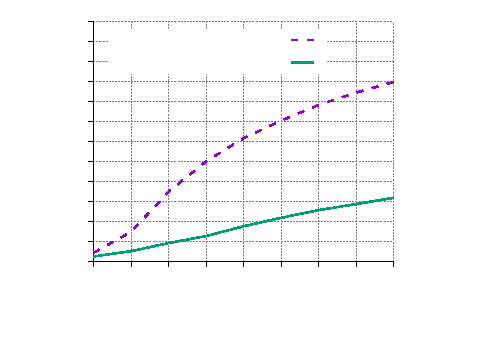
\includegraphics{figures/concat-graph-data.pdf}}%
    \gplfronttext
  \end{picture}%
\endgroup

    \end{subfigure}%
    \hspace{-20pt}
    \begin{subfigure}[t]{0.5\textwidth}
        \centering
        % GNUPLOT: LaTeX picture with Postscript
\begingroup
  \makeatletter
  \providecommand\color[2][]{%
    \GenericError{(gnuplot) \space\space\space\@spaces}{%
      Package color not loaded in conjunction with
      terminal option `colourtext'%
    }{See the gnuplot documentation for explanation.%
    }{Either use 'blacktext' in gnuplot or load the package
      color.sty in LaTeX.}%
    \renewcommand\color[2][]{}%
  }%
  \providecommand\includegraphics[2][]{%
    \GenericError{(gnuplot) \space\space\space\@spaces}{%
      Package graphicx or graphics not loaded%
    }{See the gnuplot documentation for explanation.%
    }{The gnuplot epslatex terminal needs graphicx.sty or graphics.sty.}%
    \renewcommand\includegraphics[2][]{}%
  }%
  \providecommand\rotatebox[2]{#2}%
  \@ifundefined{ifGPcolor}{%
    \newif\ifGPcolor
    \GPcolortrue
  }{}%
  \@ifundefined{ifGPblacktext}{%
    \newif\ifGPblacktext
    \GPblacktexttrue
  }{}%
  % define a \g@addto@macro without @ in the name:
  \let\gplgaddtomacro\g@addto@macro
  % define empty templates for all commands taking text:
  \gdef\gplbacktext{}%
  \gdef\gplfronttext{}%
  \makeatother
  \ifGPblacktext
    % no textcolor at all
    \def\colorrgb#1{}%
    \def\colorgray#1{}%
  \else
    % gray or color?
    \ifGPcolor
      \def\colorrgb#1{\color[rgb]{#1}}%
      \def\colorgray#1{\color[gray]{#1}}%
      \expandafter\def\csname LTw\endcsname{\color{white}}%
      \expandafter\def\csname LTb\endcsname{\color{black}}%
      \expandafter\def\csname LTa\endcsname{\color{black}}%
      \expandafter\def\csname LT0\endcsname{\color[rgb]{1,0,0}}%
      \expandafter\def\csname LT1\endcsname{\color[rgb]{0,1,0}}%
      \expandafter\def\csname LT2\endcsname{\color[rgb]{0,0,1}}%
      \expandafter\def\csname LT3\endcsname{\color[rgb]{1,0,1}}%
      \expandafter\def\csname LT4\endcsname{\color[rgb]{0,1,1}}%
      \expandafter\def\csname LT5\endcsname{\color[rgb]{1,1,0}}%
      \expandafter\def\csname LT6\endcsname{\color[rgb]{0,0,0}}%
      \expandafter\def\csname LT7\endcsname{\color[rgb]{1,0.3,0}}%
      \expandafter\def\csname LT8\endcsname{\color[rgb]{0.5,0.5,0.5}}%
    \else
      % gray
      \def\colorrgb#1{\color{black}}%
      \def\colorgray#1{\color[gray]{#1}}%
      \expandafter\def\csname LTw\endcsname{\color{white}}%
      \expandafter\def\csname LTb\endcsname{\color{black}}%
      \expandafter\def\csname LTa\endcsname{\color{black}}%
      \expandafter\def\csname LT0\endcsname{\color{black}}%
      \expandafter\def\csname LT1\endcsname{\color{black}}%
      \expandafter\def\csname LT2\endcsname{\color{black}}%
      \expandafter\def\csname LT3\endcsname{\color{black}}%
      \expandafter\def\csname LT4\endcsname{\color{black}}%
      \expandafter\def\csname LT5\endcsname{\color{black}}%
      \expandafter\def\csname LT6\endcsname{\color{black}}%
      \expandafter\def\csname LT7\endcsname{\color{black}}%
      \expandafter\def\csname LT8\endcsname{\color{black}}%
    \fi
  \fi
    \setlength{\unitlength}{0.0500bp}%
    \ifx\gptboxheight\undefined%
      \newlength{\gptboxheight}%
      \newlength{\gptboxwidth}%
      \newsavebox{\gptboxtext}%
    \fi%
    \setlength{\fboxrule}{0.5pt}%
    \setlength{\fboxsep}{1pt}%
\begin{picture}(4680.00,3276.00)%
    \gplgaddtomacro\gplbacktext{%
      \csname LTb\endcsname%%
      \put(721,751){\makebox(0,0)[r]{\strut{}$\sfrac{1}{16}$}}%
      \csname LTb\endcsname%%
      \put(721,943){\makebox(0,0)[r]{\strut{}$\sfrac{1}{8}$}}%
      \csname LTb\endcsname%%
      \put(721,1135){\makebox(0,0)[r]{\strut{}$\sfrac{1}{4}$}}%
      \csname LTb\endcsname%%
      \put(721,1327){\makebox(0,0)[r]{\strut{}$\sfrac{1}{2}$}}%
      \csname LTb\endcsname%%
      \put(721,1519){\makebox(0,0)[r]{\strut{}1}}%
      \csname LTb\endcsname%%
      \put(721,1711){\makebox(0,0)[r]{\strut{}2}}%
      \csname LTb\endcsname%%
      \put(721,1903){\makebox(0,0)[r]{\strut{}4}}%
      \csname LTb\endcsname%%
      \put(721,2095){\makebox(0,0)[r]{\strut{}8}}%
      \csname LTb\endcsname%%
      \put(721,2287){\makebox(0,0)[r]{\strut{}16}}%
      \csname LTb\endcsname%%
      \put(721,2479){\makebox(0,0)[r]{\strut{}32}}%
      \csname LTb\endcsname%%
      \put(721,2671){\makebox(0,0)[r]{\strut{}64}}%
      \csname LTb\endcsname%%
      \put(721,2863){\makebox(0,0)[r]{\strut{}128}}%
      \csname LTb\endcsname%%
      \put(721,3055){\makebox(0,0)[r]{\strut{}256}}%
      \csname LTb\endcsname%%
      \put(900,484){\makebox(0,0){\strut{}0}}%
      \csname LTb\endcsname%%
      \put(1260,484){\makebox(0,0){\strut{}}}%
      \csname LTb\endcsname%%
      \put(1620,484){\makebox(0,0){\strut{}100}}%
      \csname LTb\endcsname%%
      \put(1980,484){\makebox(0,0){\strut{}}}%
      \csname LTb\endcsname%%
      \put(2340,484){\makebox(0,0){\strut{}200}}%
      \csname LTb\endcsname%%
      \put(2699,484){\makebox(0,0){\strut{}}}%
      \csname LTb\endcsname%%
      \put(3059,484){\makebox(0,0){\strut{}300}}%
      \csname LTb\endcsname%%
      \put(3419,484){\makebox(0,0){\strut{}}}%
      \csname LTb\endcsname%%
      \put(3779,484){\makebox(0,0){\strut{}400}}%
    }%
    \gplgaddtomacro\gplfronttext{%
      \csname LTb\endcsname%%
      \put(391,1903){\rotatebox{-270}{\makebox(0,0){\strut{}}}}%
      \put(2339,154){\makebox(0,0){\strut{}Number of columns}}%
      \csname LTb\endcsname%%
      \put(3286,1118){\makebox(0,0)[r]{\strut{}implicit join}}%
      \csname LTb\endcsname%%
      \put(3286,898){\makebox(0,0)[r]{\strut{}dependent join}}%
    }%
    \gplbacktext
    \put(0,0){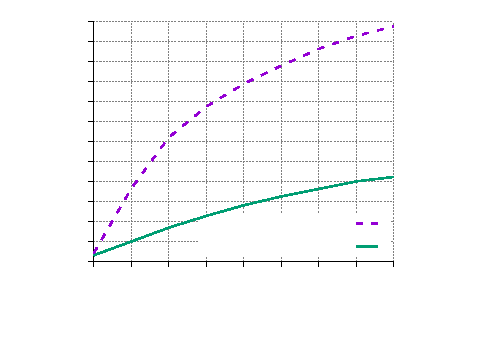
\includegraphics{figures/join-graph-data.pdf}}%
    \gplfronttext
  \end{picture}%
\endgroup

    \end{subfigure}
    \caption{#1}
    \label{fig:dependentVsImplicitBenchmarks}
  \end{figure}
}

\newcommand{\goodreducescalacodesection}{\lstinputlisting[style=scala, firstline=3, lastline=4, breaklines]{scala/src/main/scala/goodreduce.scala}}
\newcommand{\shapecodesection}{\lstinputlisting[style=scala, firstline=8, lastline=11, breaklines]{scala/src/main/scala/numpy.scala}}
\newcommand{\datatypecodesection}{\lstinputlisting[style=scala, firstline=19, lastline=19, breaklines]{scala/src/main/scala/numpy.scala}}
\newcommand{\ndarraycodesection}{\lstinputlisting[style=scala, firstline=23, lastline=23, breaklines]{scala/src/main/scala/numpy.scala}}
\newcommand{\randomnormalcodesection}{\lstinputlisting[style=scala, firstline=27, lastline=27, breaklines]{scala/src/main/scala/numpy.scala}}
\newcommand{\multiplycodesection}{\lstinputlisting[style=scala, firstline=31, lastline=31, breaklines]{scala/src/main/scala/numpy.scala}}
\newcommand{\numelementscodesection}{\lstinputlisting[style=scala, firstline=36, lastline=40, breaklines]{scala/src/main/scala/numpy.scala}}
\newcommand{\reshapecodesection}{\lstinputlisting[style=scala, firstline=44, lastline=45, breaklines]{scala/src/main/scala/numpy.scala}}
\newcommand{\reducecodesection}{\lstinputlisting[style=scala, firstline=50, lastline=66, breaklines]{scala/src/main/scala/numpy.scala}}
\newcommand{\npmeancodesection}{\lstinputlisting[style=scala, firstline=86, lastline=87, breaklines]{scala/src/main/scala/numpy.scala}}
\newcommand{\badreducescalacodesection}{\lstinputlisting[style=scala, firstline=2, lastline=4, breaklines]{scala/src/test/scala/badreduce.scala}}

\hfuzz=0.5pt

%%%%%%%%%%%%%%%%%%%%%%%%%%%%%%%%%%%%%%%%%%%%%%%%%%
%%%%%%%%%%%%%% TypeOf paper headers %%%%%%%%%%%%%%
%%%%%%%%%%%%%%%%%%%%%%%%%%%%%%%%%%%%%%%%%%%%%%%%%%

\newcommand{\oursystem}{$\lambda${\tiny $\mathop{\protect\vphantom{X}}^\text{nd}_{<:\{\}}$}\xspace}
\newcommand\FR{System~FR\xspace}
\newcommand\singleton[1]{\lbrace #1 \rbrace}
\usepackage{xfrac}
\usepackage{caption}
\usepackage{subcaption}
\usepackage{upgreek} % for \textmu


\begin{document}

\frontmatter
\begin{titlepage}
\begin{otherlanguage}{french}
\begin{center}
\sffamily
\null\vspace{2cm}
\huge Abstractions for Type-Level Programming\\[24pt]
\textcolor{gray}{\small THIS IS A TEMPORARY TITLE PAGE\\
It will be replaced for the final print by a version\\[-14pt]
provided by the registrar's office.}
\vfill
\normalsize THÈSE N. TBD (\the\year)\\[10pt]
PRÉSENTÉE LE {\MakeUppercase\today}\\
À LA FACULTÉ INFORMATIQUE ET COMMUNICATIONS\\
LABORATOIRE DE MÉTHODES DE PROGRAMMATION\\
PROGRAMME DOCTORAL EN INFORMATIQUE ET COMMUNICATIONS\\[10pt]
ÉCOLE POLYTECHNIQUE FÉDÉRALE DE LAUSANNE\\
pour l'obtention du grade de Docteur ès Sciences\\
par\\[20pt]
\Large Olivier Blanvillain\\[20pt]
\small acceptée sur proposition du jury:\\[4pt]
Prof Name Surname, président du jury\\
Prof Name Surname, directeur de thèse\\
Prof Name Surname, rapporteur\\
Prof Name Surname, rapporteur\\
Prof Name Surname, rapporteur\\[12pt]
Lausanne, EPFL, \the\year
\end{center}
\vspace{2cm}
\end{otherlanguage}
\end{titlepage}


\setcounter{page}{0}

\chapter{Acknowledgements}

I would like to thank my advisor, Martin Odersky, for his help and support throughout my PhD studies, and for providing me with this unique opportunity to work on my favorite language.

I would also like to thank the other members of my thesis committee, Paolo Giarrusso, Richard Eisenberg, and Viktor Kuncak, for agreeing to review my dissertation and taking part in the committee.

I would like to thank all my colleagues from LAMP, LARA and Scala Center.
You were the source of so many interesting discussions, cheerful moments, and great memories, it was really a pleasure to work along your side.
Aggelos Biboudis,
Aleksander Boruch-Gruszecki,
Allan Renucci,
Anatolii Kmetiuk,
Darja Jovanovic,
Denys Shabalin,
Dmitry Petrashko,
Dragana Milovancevic,
Fabien Salvi,
Felix Mulder,
Fengyun Liu,
Georg Schmid,
Guillaume Martres,
Guillaume Masse,
Heather Miller,
Jad Hamza,
Jamie Thompson,
Jonathan Brachthäuser,
Jorge Vicente,
Julien Richard-Foy,
Matthieu Bovel,
Maxime Kjaer,
Natascha Fontana,
Nicolas Stucki,
Ólafur Geirsson,
Paolo Giarrusso,
Romain Edelmann,
Sandro Stucki,
Sébastien Doeraene,
Travis Lee---thank you!
If it wasn't for you, I would have not have gotten here.

A special thanks to Georg Schmid for being such an amazing friend, colleague and co-author over the past five years.
I will never forget what we went through together, the paper deadlines, the bike rides, the hacking sessions, the games...
It's crazy how much we did and learned together.
And of course, thank you Mia Primorac for being there for all the fun parts!

I would like to thank my parents, Soledad and Christian, and my little sister, Alicia, for being there for me all these years.
It was truly a chance and a pleasure to have you close by throughout my PhD.
I must also thank the latest arrival in family, Leila, for being such an endless source of joy, cuteness and distraction.

Last but not the least, I would like to thank Dragana for being always there on my side, for being so kind and patient, and for her tremendous help in putting the ideas of this thesis into text.
You are the best.


\bigskip
\noindent\textit{Lausanne, \today}
\hfill Olivier Blanvillain

\cleardoublepage
\chapter*{Abstract} % max 3499 characters
\markboth{Abstract}{Abstract}
\addcontentsline{toc}{chapter}{Abstract (English/Français)}

Over the past decade, the Scala community has shown great interest in using type-level programming to obtain additional type safety.
Unfortunately, the lack of support from the Scala compiler has been a barrier to the adoption of that technique, notably due to its negative impact on compilation times.
In this thesis, we present three techniques for type-level programming in Scala.
First, we explain the status quo, implicits, and show how we can divert them from their intended use to write ad hoc type-level programs.
Second, we propose a generalization of Scala's singleton types, which adds the ability to manipulate term-level programs at the type level.
Third, we introduce match types, a type-level equivalent of pattern matching, which we implemented in the Scala~3 compiler.
Throughout this dissertation, we demonstrate the practicality of our newly introduced techniques, by the means of case studies and examples.
Our performance evaluation shows that our new techniques outperform the status quo in terms of binary sizes and compilation times.

\paragraph{Keywords} Programming Languages, Type Systems, Compilers, Scala.

\begin{otherlanguage}{french}
\cleardoublepage
\chapter*{Résumé}
\markboth{Résumé}{Résumé}

Au cours de la dernière décennie, la communauté Scala a montré un grand intérêt pour l'utilisation de la programmation au niveau du système de type afin d'améliorer la sûreté du typage.
Malheureusement, le manque de support dans le compilateur Scala a été un frein pour l'adoption de cette technique, notamment en raison de son impact négatif sur les temps de compilation.
Dans cette thèse, nous présentons trois techniques de programmation au niveau du système de type en Scala.
Tout d'abord, nous expliquons le statu quo, les implicites, et montrons comment nous pouvons les détourner de leur usage prévu pour écrire des programmes au niveau des types.
Deuxièmement, nous proposons une généralisation des types singleton de Scala, qui ajoute la possibilité de manipuler et d'exécuter des programmes au niveau des types.
Troisièmement, nous introduisons les match types, un équivalent du pattern matching au niveau des types, que nous avons implémenté dans le compilateur Scala~3.
Tout au long de cette dissertation, nous démontrons le caractère pratique de nos nouvelles techniques, au moyen d'études de cas et d'exemples.
Notre évaluation des performances montre que nos nouvelles techniques surpassent le statu quo en termes de tailles binaires et de temps de compilation.

\paragraph{Mots clés} Langages de Programmation, Systèmes de Types, Compilateurs, Scala.

\end{otherlanguage}

\hypersetup{linkcolor=black}
\tableofcontents
\cleardoublepage
\phantomsection
\addcontentsline{toc}{chapter}{List of Figures}
\listoffigures
\hypersetup{linkcolor=purplish}
\mainmatter

%%%%%%%%%%%%%%%%%%%%%%%%%%%%%%%%%%%%%%%%%%%%%%%%%%
%%%%%%%%%%%%%%%%  Thesis Content  %%%%%%%%%%%%%%%%
%%%%%%%%%%%%%%%%%%%%%%%%%%%%%%%%%%%%%%%%%%%%%%%%%%

\chapter{Introduction}
\label{chap:introduction}

In March 2017, our research group went on a ski retreat in the Swiss Alps.
After a full day of skiing on the Diablerets massif, we gathered for a lab dinner.
Denys Shabalin, who was working on Scala Native at the time~\citep{shabalin2020just}, started a conversation about manual memory management.
The discussion revolved around the following question: could a Rust-like ownership system be viable for Scala?
Denys' answer was clear: ownership is fundamentally at odds with the way Scala handles references, and without making deep changes to Scala's type system, the task was simply impossible.

The next day, I came up with a toy domain-specific language (DSL) that implements the basis of a linear type system using type-level programming.
Here is an example of a short program written in this DSL:

\memImplicitMain

\noindent
The type argument of |Context| is a type-level list of strings that corresponds to the memory regions allocated at each program point.
Methods of |Context| use type-level programming techniques to enforce the following properties:

\begin{enumerate}
  \item memory regions must be allocated (|malloc|) \emph{before} they are deallocated (|free|),
  \item all memory regions must be deallocated by the end of the program,
  \item dereferencing (|deref|) is only allowed on previously allocated regions.
\end{enumerate}

\noindent
The implementation makes use of Scala's implicits to enforce these properties.
While this small DSL is obviously too simplistic to be of any practical use, it demonstrates the power of type-level programming.

I was delighted with my solution!
Denys, however, was not impressed.
I attribute this apathy to his dislike of implicits.
Despite their widespread usage, implicits are notorious for their complexity~\citep{kvrikava2019scala}.
In particular, using implicits for type-level computations requires carefully crafted definitions following a specific pattern.
To give the reader a glimpse of this pattern, we show the definition of the |free| method on |Context|:

\memImplicitContextFree

\noindent
This definition uses three parameter lists, one for type parameters (|V| and |Out|), one for a value parameter (|v|), and one of an implicit value parameter (|ev|).
Only the second parameter list is intended to be specified at use site; the type and implicit parameters are meant to be inferred.
When a users write |.free("mem")| they only set the |v| parameter (|v="mem"|); the compiler takes care of finding valid assignments for |V|, |Out| and |ev|.
The implicit parameter of type |Remove[V,Ps,Out]| is the entry point to the world of type-level programming.
It specifies how |V| (constrained by to be |v|'s type), |Ps| (defined in the class), and |Out| (unconstrained) are interrelated:

\memImplicitRemove

\noindent
Implicit-prefixed definitions can be understood as \emph{facts} and \emph{rules} of a logic program.
The first definition, |casehead|, specifies a fact: the result of removing |V| from the list |V::Ps| is |Ps|, which is expressed as an instance of |Remove[V,V::Ps,Ps]|.
The second definition, |casetail|, specifies a rule: if the result of removing |V| from the list |Pt| is |Out|, the results of removing |V| from the list |Ph::Pt| is |Ph::Out| (\Cref{sec:hlists-remove} develops this example in more details).
When a user writes |ctx.free("mem")| on a |ctx| of type |Context["bool"::"mem"::HNil]|, the compiler uses |casehead| and |casetail| to compute a type |Out| such that |Out| is the results of removing |"mem"| from |"bool"::"mem"::HNil|.

In retrospect, I have to agree with Denys' judgment at the time: this style of programming is convoluted, to say the least.
Aesthetics and pragmatism aside, programming with implicits requires a complete paradigm shift.
Instead of using pattern matching and functions, implicits require algorithms to be expressed using relations and constraints, which makes the task harder than it should be.

\emph{Can we do better?} This is the question that motivates the work presented in this dissertation.

Our contributions are as follows:

\begin{itemize}
  \item In \Cref{chap:ab-using-implicits}, we present techniques for programming at the type-level with implicits.
  In particular, we develop the example presented in the introduction, and show how to use Scala's implicit resolution mechanism to compute types, in a style that resembles logic programming.

  \item In \Cref{chap:generalizing-singleton-types}, we propose a generalization of Scala's singleton types, whose goal is to enable type-level programming in an accessible style.
  Concretely, we extend Scala's type system with the ability to lift term-level programs to the type level and evaluate those programs during type-checking.
  We implement our system as an extension of the Scala~3 compiler, and show its practicality with a case study in which we develop a strongly-typed interface for Spark datasets.

  \item In \Cref{chap:match-types}, we introduce match types, a type-level equivalent of pattern matching.
  Match types integrate seamlessly into programming languages with subtyping and, despite their simplicity, offer significant additional expressiveness.
  We formalize match types in a self-contained calculus based on \SystemFsub and prove its soundness.
  We demonstrate the practical value of our system by implementing match types in the Scala~3 compiler, thus making type-level programming readily available to a broad audience of programmers.

  \item In \Cref{chap:type-safe-regular-expressions}, we propose a new design for type-safe regular expressions in Scala.
  Our approach makes extensive use of match types to identify capturing groups during type checking.
  We walk the reader through our design, step by step, providing detailed explanations along the way.
  Our implementation is on par with Java's regular expressions and only has a marginal impact on compilation times.

  \item In \Cref{chap:performance-evaluation}, we evaluate the performance of the various type-level programming techniques introduced in prior chapters, when confronted with large type-level programs.
  We show that the techniques introduced in \Cref{chap:generalizing-singleton-types} and~\ref{chap:match-types} systematically outperform implicits in terms of compilation times and binary sizes.
\end{itemize}

\chapter{(Ab)Using Implicits}
\label{chap:ab-using-implicits}

Scala's implicit parameters have outgrown their roots as a simple syntactic construct to the extent that they provide basic support for type-level programming.
In this chapter, we present techniques for implicit-based type-level programming in Scala.
In particular, through extended examples, we show how to use Scala's implicit resolution mechanism to compute types, in a style that resembles logic programming.

\subsection*{Attribution}

The first section of this chapter is based on the introduction to implicits from~\citep{odersky2018simplicitly}, which was written in collaboration with Martin Odersky, Fengyun Liu, Aggelos Biboudis, Heather Miller and Sandro Stucki, and published in POPL'18.

Code samples for the remaining of this chapter are based on the implementation of heterogeneous lists from the Shapeless library~\citep{sabin2011shapeless}.

\section{Implicit Parameters: Overview}

\emph{Implicit parameters} offer a convenient way to write code without the need to pass all arguments explicitly.
The ability to omit function arguments gives rise to many interesting coding styles and patterns.
On every call to functions with implicit parameters, the compiler looks for an implicit definition in scope to satisfy the call.
So, instead of passing a parameter explicitly:

\explicitModulo

\noindent
we can mark a set of parameters as implicit (a single parameter in this example) and let the compiler retrieve the missing argument for us.
In the following example, |addm| is a method with one implicit parameter and |modulo| is an implicit definition:

\implicitModulo

The process of implicit parameter discovery performed by the compiler is called \emph{implicit resolution}.
The resolution algorithm looks for implicits in the current scope and in the companion objects of all classes associated with the query type.
In the previous example, the implicit definition is declared in the current scope.
Since that definition has type |Int|, the compiler resolves the method call by passing |modulo| automatically.

\subsubsection{The type class pattern}

Implicits can be used to implement type classes~\citep{wadler1989how} as a design pattern~\citep{oliveira2010type}.
We give an example of an implementation of the |Ordering| type class.
This example consists of three parts:

\begin{enumerate}
  \item |Ordering[T]|, which is a regular trait with a single method, |compare|,
  \item the generic function |comp|, which compares two arguments and accepts an implicit argument, providing an \emph{implicit evidence} that these two values can be compared,
  \item the implicit definition |intOrdering|, which provides an \emph{instance} of the |Ordering| type class for integers.
\end{enumerate}

\ordExample

We have briefly introduced implicit parameters and showed how they can be used to avoid clutter in function applications.
In the next section, we present recursive implicit resolution.

\section{Recursive Implicit Resolution}
\label{sec:recursive-implicit-resolution}

Implicit methods can themselves take implicit parameters.
For example, we can define the lexicographic list ordering as follows:

\ordListExample

\noindent
This definition is parametrized by the list's element type and by an ordering of that type, passed as an implicit parameter.
Since |listOrdering| is itself implicit, it defines a \emph{rule}: it allows the compiler to materialize an implicit of type |Ordering[List[T]]| given an implicit type |Ordering[T]|, for any type |T|.

Parametrized implicit definitions can lead to recursive implicit resolution. For example, the compiler will use |listOrdering| twice to synthesize an implicit |Ordering[List[List[T]]]|.
This is where the (type-level) fun begins!

\subsubsection{Heterogeneous lists}

A heterogeneous list, or |HList| for short~\citep{kiselyov2004strongly}, is a datatype capable of storing data of different types.
In Scala~3, we can define the |HList| datatype as follows:

\hlistEnumDefinition

\noindent
The |::| constructor offers an interesting symmetry between the term and type level, which allows |HList| types to capture the same structure that their term-level counterparts.
For example, the term |::(1,::(2,HNil()))| can be typed as |::[1,::[2,HNil]]|, which is a perfect reification of that term (we use literal singleton types to represent constant literals at the type level~\citep{leontiev2014sip}).

\subsubsection{HList's remove}
\label{sec:hlists-remove}

Scala's implicits allow us to define type-level operations for heterogeneous lists.
We develop the example presented in \Cref{chap:introduction} by looking into the remove operation on |HList|s.
The remove operation takes as argument an element and a list, and returns that list with the first occurrence of the element removed.
This operation should yield an error if the element is not part of the list.

An implicit-based type-level operation typically takes the form of a trait, the operation's entry point, and several implicit definitions, one for each "case" of the operation's algorithm.
Let us consider the implementation of the remove operation in more detail:

\memImplicitRemove

\noindent
The |Remove| trait takes 3 type parameters: 2 inputs, |V| (the element to remove) and |Ps| (the list), and one output, |Out| (the list, with the element removed).
The two implicit definitions, |casehead| and |casetail|, correspond to the base case and the recursive case of the list removal operation, respectively.
The right-hand side of those definitions is devoid of meaning, instances of the |Remove| trait merely act as placeholders (the type parameters of those constructor calls are inferred from their expected type).
The |Remove| trait is intended to be used as an implicit parameter, with constrained input types, and an unconstrained output type.

When the given element is not part of the list, implicit resolution fails with an "implicit not found" error, which indicates the incorrect use of |Remove|.
More precisely, the implicit search first iterates through the list by repeatedly using |casetail| until it reaches the end of the list, at which point it fails to find an implicit value of type |Remove[V,HNil,Out]| (neither |casehead| nor |casetail| produce an instantiation of |Remove| with |Ps=HNil|).

As an example usage of |Remove|, consider the following stringly-typed, JavaScript-inspired method:

\addEventListenerJS

\noindent
This method's documentation specifies 5 valid alternatives for the |event| argument, but that constraint is not reflected in the method's type signature.
In JavaScript, calling this method with an erroneous element event type is a \emph{no-op}, which can make this kind of error particularly hard to spot.

Instead of specifying that constraint in the documentation, we can represent the valid event types in a |HList|, and use an implicit parameter of type |Remove| to statically enforce that property:

\addEventListenerImplicitDef

\noindent
The |Singleton| type bound is a marker that instructs type inference to preserve union types and literal singleton types (by default, the compiler widens those types).
The "|?|" type is Scala~3's new syntax for wildcard types~\citep[Wildcard Arguments in Types]{odersky2013scala}.

With this updated signature, the compiler is able to detect invalid event types at compile time.
When given a valid event type |E|, the compiler synthesizes an implicit evidence of type |Remove[E,EventTypes,?]| which witnesses |E|'s validity.
After implicit resolution, calls to the |addEventListener| method are expanded to automatically insert an implicit parameter for the second parameter list, such as in the following example:

\addEventListenerImplicitCall

This concludes our presentation of the implicit-based encoding of type-level computation.
Despite its verbosity, this pattern generalizes to arbitrary recursive computations and enables Scala programmers to write elaborate type-level programs solely based on implicits.
In the next section, we discuss ambiguities and priorities between implicit definitions.

\section{Ambiguities and Priorities}

Scala's implicit resolution relies on an intricate priority system to establish the precedence of implicit definitions.
Implicit-based programs sometimes rely on ambiguities and priorities of implicit definition, as we will see in this section through a series of examples.

\subsection{Implicit Ambiguities}
\label{subsec:implicit-ambiguities}

The Scala compiler rejects programs with \emph{ambiguous} implicit definitions.
For instance, if we write two identically-typed implicit definitions in the same scope, the compiler will consider them ambiguous and report an error:

\implicitAmbiguity

While ambiguities typically indicate programming errors, we can also use them purposefully to implement error cases of a type-level program.
As an example, consider the |NotIn| operation on |HList| that is only defined if the given element is \emph{not} part of the list.
We define |NotIn| using two ambiguous implicits; the implementation is lengthy, but straightforward:

\memImplicitNotIn

\noindent
The |casenil| and |casecons| implicits simply iterate through the list.
The |ambiguous| implicits are two identical definitions that will cause the compiler to raise an error if |V| and |Ph| are equal, for any element |Ph| of the list ("|=:=|" is a type from Scala's standard library that witnesses mutual subtyping).

As an example usage of |NotIn|, we revisit the DSL presented in \Cref{chap:introduction}.
Programs in our DSL consist of sequences of method calls on a |Context|, which tracks the memory regions that are currently allocated in the program, using a |HList| of names.
We use the |NotIn| operation to constrain the allocation method, |malloc|, to prevent allocating regions with already used names:

\memImplicitContextMalloc

Scala~3 introduced an alternative to the ambiguous implicit pattern in the form of the |scala.util.NotGiven| type~\citep[Given Instances]{odersky2013scala}.
The compiler will synthesize an implicit parameter of type |NotGiven[T]| if and only if there is no implicit value of type |T| in scope.
We can use a "negative" implicit evidence to simplify the definition of |NotIn| by removing the ambiguous implicits and changing |casecons| to the following:

\memImplicitNotGiven

\subsection{Implicit Priorities}
\label{subsec:implicit-priorities}

When looking for implicits, the Scala compiler visits scopes sequentially, in a precisely defined order.
At any point in the search, if the implicits defined in the subset of scopes considered so far can fulfill the implicit query, the search succeeds and immediately terminates.
This incremental process has two consequences.
First, it allows the compiler to efficiently look for implicits by naturally pruning the search space.
Second, it provides an ad-hoc mechanism to disambiguate implicits.
Scala programmer can artificially partition their implicit definitions into multiple scopes to implement a priority system.

Let us consider an example of operation on |HList| whose implementation uses implicit priorities.
|RemoveAll| is a generalization of |Remove| that removes every occurrence of the given element instead of the first occurrence.
The implicit-based implementation takes the form of a trait with 3 type parameters: 2 inputs, |V| (the element to remove) and |Ps| (the list), and one output, |Out| (the list, with the elements removed):

\removeAllDefinition

From an algorithmic standpoint, we can implement |RemoveAll| as a recursive function with 3 cases, a base case for the empty list (|casenil|), a recursive case for when the head of the list matches the element to remove (|casematch|), and another recursive case for when the head doesn't match (|casedoesnt|):

\removeAllBroken

This direct implementation of |RemoveAll| using implicit definitions is, unfortunately, incorrect.
The issue is that the |casematch| and |casedoesnt| definitions are ambiguous when the head of the list matches the element to remove.
To work around that ambiguity, we split those definitions into two different scopes, so that the compiler always tries to apply the more specialized case (|casematch|) before considering the less specialized case (|casedoesnt|).
Concretely, we define low priority implicits in a separate trait, and have |RemoveAll|'s companion object extend that trait:

\removeAllPrioritized

In Scala~3, the rules for implicit ambiguities changed to take implicit parameters into account, thus introducing another, more direct, disambiguation mechanism.
All else being equal, an implicit definition that takes implicit parameters is considered less specific than an implicit definition does not take implicit parameters~\citep[Changes in Implicit Resolution]{odersky2013scala}.
As a result, implicit-based type-level programs written in Scala~3 do not need to use the patterns of ambiguities and priorities presented in this section (\ref{subsec:implicit-priorities} and \ref{subsec:implicit-ambiguities}).

\section{Conclusion}

In this chapter, we presented several techniques for type-level programming with implicits.
This style of programming is, unfortunately, quite cumbersome.
In addition to the heavy syntax, type-level programming with implicits also requires a deep understanding of the implicit resolution algorithm.
As we will see in \Cref{chap:performance-evaluation}, those techniques come at a high cost in terms of compilation time, which hinders their usability on a large scale.
Yet, despite those shortcomings, Scala programmers have shown a persistent interest in this style of programming, as demonstrated by its popularity in the open-source community~\citep{sabin2011shapeless, pilquist2013scodecs, blanvillain2016frameless}.

\chapter{Generalizing Scala's Singleton Types}
\label{chap:generalizing-singleton-types}

Type-level programming is an increasingly popular way to obtain additional type safety.
Unfortunately, it remains a second-class citizen in the majority of industrially-used programming languages.
We propose a new dependently-typed system with subtyping and singleton types whose goal is enabling type-level programming in an accessible style.
To this end, we have prototyped our system as an extension of the Scala programming language.
We demonstrate the practicality of our system with a case study in which we develop a strongly-typed interface for Spark datasets.
Through our formalization and implementation in the context of an industrial-strength compiler, we hope to provide valuable insights for language designers interested in dependent types.

\subsection*{Attribution}

This chapter is based on~\citep{schmid2020coming}, which was written in collaboration with Georg Schmid, Jad Hamza, and Viktor Kuncak.
Georg and I worked hand-in-hand on this project: we collaborated through countless whiteboard discussions and pair programming sessions, which resulted in shared first authorship of the implementation and most of the text.
The said report covers more material than what is included in this chapter, in particular, our formalization and the associated metatheory are out of the scope of this dissertation.

\section{Introduction}

Dependent types have been met with considerable interest from the research community in recent years.
Their primary application so far has been in proof assistants such as Coq~\citep{bertot2004interactive} and Agda~\citep{norell2007towards}, where they provide a sound and expressive foundation for theorem proving.
However, dependent types are still largely absent from general-purpose programming languages, despite a long history of lightweight approaches~\citep{xi1998eliminating}.
In the context of Haskell, much research has gone into extending the language to support computations on types, for instance in the form of functional dependencies~\citep{jones2000type}, type families~\citep{kiselyov2010fun} and promoted datatypes~\citep{yorgey2012giving}.
These techniques have seen vivid adoption by Haskell programmers, showing that there is a real demand for such mechanisms.
Furthermore, recent research has explored how dependent types could be added to the language for the same purpose~\citep{eisenberg2016dependent, weirich2017a}.

Dependently-typed languages often rely on a unified syntax to describe both terms and types.
The simplicity of this approach is unfortunately at odds with the design of most programming languages, where types and terms are expressed using separate syntactic categories.
Singleton types provide a simple solution to this problem by allowing terms to be represented as types.

In this chapter, we report on our attempt to generalize Scala's singleton types to support type-level programming, as well as a lightweight form of dependently-typed programming.
Unlike proof assistants, we do not aim to use types as a general-purpose logic, which would favor designs ensuring the totality of functions through termination checks.
Instead, our focus is on improving type safety by increasing the expressive power of the type system.

With these goals in mind, we extended Scala's type system to lift programs to the type level and partially evaluate them as part of type-checking.
Users can manipulate those types either directly, using new syntactic forms in Scala's type language, or have them inferred automatically using a new language keyword.
This effectively allows users to execute programs involving functions and pattern matching at the type level.

The remaining of the chapter is organized as follows:

\begin{itemize}
\item
  We begin by motivating why type-level programming is desirable and how one might use our Scala extension to improve type safety (\Cref{sec:motivating-example}). Our example demonstrates how to design a strongly-typed API in a functional style accessible to programmers.
\item
  We describe how we extended Scala with a generalization of singleton types (\Cref{sec:extending-scala}).
  We prototyped our type system on top of Dotty, the reference Scala~3 compiler.
  This practical introduction would be of interest to any Scala programmer willing to learn how to use our system, as well as programming language designers interested in dependent types.
\item
  We show a concrete use-case of our system by implementing a strongly-typed wrapper for Apache Spark~\citep{zaharia2016apache} (\Cref{sec:use-case}).
  Thanks to our generalized singleton types, we can statically ensure the type safety of database operations such as join and filter.
  We compare our implementation with an equivalent implicit-based one and show remarkable compilation time savings.
\end{itemize}

Our original presentation of generalized singleton types contains a formalization \citep[Section 3 and 4]{schmid2020coming}, which is out of the scope of this chapter.

\section{Motivating Example}
\label{sec:motivating-example}

We begin by motivating why type-level programming is desirable in general purpose programming.
In our first example, we design an API that keeps track of database tables' schemas in the type, and uses that information to improve type safety.
The examples in this section are written in our Scala extension described in \Cref{sec:extending-scala}.

As a first step, we show how our system supports type-level programming in the style of term-level programs.
Consider the following definition of the list datatype, which is standard Scala up the |dependent| keyword:

\begin{lstlisting}
sealed trait Lst { (*\text{\dots}*) }
dependent case class Cons(head: Any, tail: Lst) extends Lst
dependent case class Nil() extends Lst
\end{lstlisting}

\noindent
We can define list concatenation in the usual functional style of Scala, that is, using pattern matching and recursion:

\begin{lstlisting}
sealed trait Lst:
  dependent def concat(that: Lst) <: Lst =
    this match
      case Cons(x, xs) => Cons(x, concat(xs, that))
      case Nil() => that
\end{lstlisting}

\noindent
By annotating a method as |dependent|, the user instructs our system that the result type of |concat| should be as precise as its implementation.
Effectively, this means that the body of |concat| is lifted to the type level in a singleton type, and will be partially evaluated at every call site to compute a precise result type which \emph{depends} on the given inputs.
For recursive |dependent| methods such as |concat|, we infer types that include calls to |concat| itself.
The |<:| annotation lets us provide an upper bound on |concat|'s result type, which will be used while type checking the method's definition.
Finally, by qualifying the definition of |Cons| and |Nil| as |dependent|, we also allow their constructors and extractors to be lifted to the type level.
Using these definitions, we can now request the precise type whenever we manipulate lists by annotating |val| bindings as |dependent|:

\begin{lstlisting}
dependent val l1 = Cons("A", Nil())
dependent val l2 = Cons("B", Nil())
dependent val l3 = l1.concat(l2)
l3.size: { 2 }
l3: { Cons("A", Cons("B", Nil())) }
\end{lstlisting}

Enclosing a pure term in braces (|{|~\ldots{}~|}|) denotes the singleton type of that term.
In the last two lines of this example, we are therefore asking our system to prove that |l3| has size 2 and is equivalent to |Cons("A", Cons("B", Nil()))|.
Similarly, we can define remove on |Lst|:

\begin{lstlisting}
sealed trait Lst:
  dependent def remove(e: String) <: Lst =
    this match
      case Cons(head, tail) =>
        if (e == head) tail
        else Cons(head, tail.remove(e))
      case _ => throw new Error("element not found")
\end{lstlisting}

\noindent
Removing |"B"| yields the expected result, while trying to remove |"C"| from |l3| leads to a \emph{compilation error}, since the given program will provably fail at runtime.

\begin{lstlisting}
l3.remove("B"): { Cons("A", Nil()) }
l3.remove("C") // Error: element not found
\end{lstlisting}

The lists we defined so far can be used to implement a type-safe interface for database tables:

\begin{lstlisting}
dependent case class Table(schema: Lst, data: spark.DataFrame):
  dependent def join(right: Table, col: String) <: Table =
    val s1 = this.schema.remove(col)
    val s2 = right.schema.remove(col)
    val newSchema = Cons(col, s1.concat(s2))
    val newData = this.data.join(right.data, col)
    new Table(newSchema, newData)
\end{lstlisting}

\noindent
In this example, we wrap a Spark's |DataFrame| in the |dependent| class |Table|.
The first argument of this class represents the schema of the table as a precisely-typed list.
The second argument is the underlying |DataFrame|.
In the implementation of |join|, we execute the join operation on the underlying tables (|newData|) and compute the resulting schema corresponding to that join (|newSchema|).
By annotating the |join| method as |dependent|, the resulting schema is reflected in the type:

\begin{lstlisting}
dependent val schema1 = Cons("age", Cons("name", Nil()))
dependent val schema2 = Cons("name", Cons("unit", Nil()))
dependent val table1  = Table(schema1, (*\text{\dots}*))
dependent val table2  = Table(schema2, (*\text{\dots}*))
dependent val joined  = table1.join(table2, "name")
joined: { Table(Cons("name", Cons("age", Cons("unit", Nil()))), _: DataFrame) }
\end{lstlisting}

\noindent
Reflecting table schemas in types increases type safety over the existing weakly-typed interface.
For instance, it becomes possible to raise compile-time errors when a user tries to use non-existent columns.
This is an improvement over the underlying Spark implementation that would instead fail at runtime.

\section{Implementation}
\label{sec:extending-scala}

In this section we give an overview of how we extended Scala with a generalized notion of singleton types, and how we manipulate these types during type-checking.
Our presentation is divided into three parts.

First, we introduce new types that reflect a subset of Scala's term language at the type level, and give an informal description of our type evaluation algorithm.
We then introduce the |dependent| qualifier, which influences type inference to assign generalized singleton types to the annotated definition.
Finally, we discuss how our extension interacts with other aspects of Scala, such as side effects, virtual dispatch, and recursion.

This development was an experiment to explore the feasibility of adding a lightweight form of dependent types to Scala.
We implemented our prototype as an extension of Dotty, the reference Scala~3 compiler.

\subsection{Reflecting Terms in Types}

The fundamental difference between our and Scala's existing type system is that we take Scala's notion of singleton types, that is, precise types for variable bindings and literals, and extend them to cover Scala's core functional expressions.
Concretely we add new types for the following constructs:

\begin{itemize}
  \item Variable bindings and member selections
  \item Primitive literals
  \item Method calls
  \item If-then-else expressions
  \item Pattern matching expressions
  \item Constructor calls
\end{itemize}

These new types can be expressed using the |{| $e$ |}| type syntax, where $e$ is an expression in the core functional subset of Scala listed above.
For instance, suppose $\text{foo}$ stands for the expression

\begin{lstlisting}
if (x % 2 == 0) "even" else "odd"
\end{lstlisting}

\noindent then $\text{foo}$ can be typed as |{| $\text{foo}$ |}|.
More precisely, |{| $\text{foo}$ |}| is the singleton type of $\text{foo}$ and corresponds to the unique value of $\text{foo}$ in a given context.

The first two constructs in this list have antecedents in Scala.
Types for bindings are available since the early days of Scala with the |x.type| syntax \citep[Section 3.2.1]{odersky2006scala}, which is equivalent to |{ x }| in our system.
Types for primitive literals have recently been added to the language: literals for booleans, strings and the various numeric types are made available in the type language \citep{leontiev2014sip}.

In addition to base types and singleton types for every pure term, our system also supports types that lie in-between. We add a new form, |_: T|, which supplements expressions in types of form |{| $e$ |}| by allowing the user to intersperse terms and base types.

For instance, consider the following list and its singleton type:

\begin{itemize}
  \item |Cons(Nil, Nil): { Cons(Nil, Nil) }|
\end{itemize}

In our system, this term may also be typed less precisely, such as:

\begin{itemize}
  \item |Cons(Nil, Nil): { Cons(_: Any, Nil) }|
  \item |Cons(Nil, Nil): { Cons(Nil, _: Lst) }|
  \item |Cons(Nil, Nil): { Cons(_: Any, _: Lst) }|
\end{itemize}

\noindent
all of which are subsumed by

\begin{itemize}
  \item |Cons(Nil, Nil): Lst|.
\end{itemize}

\subsection{Type Evaluation}

Our system evaluates types using a call-by-value partial evaluator, which we embedded in the type-checker.
The evaluation rules for the term in generalized singleton types are completely standard up to dynamic type tests.

We perform evaluation of types during subtyping.
For instance, consider the following definition of a |parity| function:

\begin{lstlisting}
dependent def parity(x: Int) =
  if (x % 2 == 0) "even" else "odd"
\end{lstlisting}

\noindent
In order to prove the well-typedness of

\begin{lstlisting}
val p: { "odd" } = parity(5)
\end{lstlisting}

\noindent
the type-checker will ensure that |{ parity(5) }| is a subtype of |{ "odd" }|.
In the process, the left-hand side is evaluated as follows:

\begin{lstlisting}
  { parity(5) }                          (*$(1)$*)
= { if (5 % 2 == 0) "even" else "odd" }  (*$(2)$*)
= { if (false) "even" else "odd" }       (*$(3)$*)
= { "odd" }
\end{lstlisting}

\noindent
In (1), the method call to |parity| is replaced by its result type, where the method parameter has been substituted by the singleton type of the argument, |{ 5 }|.
(2) evaluates the boolean expression to |false|.
(3) reduces the |if| expression to its else branch.

In general, our evaluator will execute operations on concrete primitive values of types such as |Boolean|, |Int| and |String|, i.e., perform constant-folding.

\subsection{Pattern Matching}
\label{pattern-matching}

Pattern matching in Scala supports a wide range of matching techniques~\citep{emir2007matching}.
For example, \emph{extractor patterns} rely on user-defined methods to extract values from objects.
As a result, these custom extractors can contain arbitrary side effects.
Our implementation limits the kind of patterns available in types to the two simplest forms: decomposition of case classes and the type-tests/type-casts patterns.

During type normalization, our system evaluates pattern matching expressions according to Scala's runtime semantics.
Patterns are checked top-to-bottom, and type-tests are evaluated using runtime type information available after type erasure.

For example, consider the following pattern matching expression:

\begin{lstlisting}
s match {
  case _: T1 => v1
  case _: T2 => v2
}
\end{lstlisting}

\noindent
When used in a type, this expression reduces to |v1| if the scrutinee's type is a subtype of |T1|.
In order to reduce to |v2|, type normalization must make sure |T1| and the scrutinee's type are disjoint, namely that the dynamic type of |s| cannot possibly be smaller than |T1|.
Disjointness proofs are built using static knowledge about the class hierarchy, such as the |sealed| and |final| qualifiers, which are Scala's way of declaring closed-type hierarchies.

\subsection{Two Modes of Type Inference}

In order to retain backwards-compatibility, our system supports two modes of type inference: the precise inference mode which infers singleton types, and the default inference mode that corresponds to Scala's type-inference algorithm.
Concretely, users opt into our new inference mode using the |dependent| qualifier on methods, values, and classes.

When inferring the result type of a |dependent| method, our system lifts the method's body into a generalized singleton type.
This lifting will be precise for the subset of expressions that is representable in types, and approximative for the rest.
When we encounter an unsupported construct, we compute its type using the default mode, yielding a type |T| which we then integrate in the lifted body as |_: T|.

For example, given the following definition:

\begin{lstlisting}
dependent def getName(personalized: Boolean) =
  if (personalized) readString() else "Joe"
\end{lstlisting}

\noindent
our system infers the following result type:

\begin{lstlisting}
{ if (personalized) (_: String) else "Joe" }
\end{lstlisting}

\noindent
We could have equivalently defined |getName| by omitting the |dependent| qualifier and writing its result type  explicitly.

Scala requires recursive methods to have an explicit result type, and this restriction also applies to |dependent| methods.
However, in the case of a |dependent| method, an explicit result type is only used as an upper bound for the actual precise result type and will only be used to type-check the method's body.
At other call sites, the (precise) inferred result type is used.
Bounds of dependent methods are written using a special syntax (|<: T|).

\subsection{Approximating Side Effects}

Scala's type system permits uncontrolled side effects in programs.
Given the absence of an effect system, result types of methods do not convey any information about the potential use of side effects in the method body.
The situation is analogous for |dependent| methods.
Since we uniformly approximate all side effects, we avoid the situation where a type refers to a value that may be modified during the program execution.
For instance, if |z| is a mutable integer variable, we will never introduce |z| in a singleton type.
However, we can still assign singleton types to expressions containing |z|, for example, we can type |Cons(z, Nil())| as |{ Cons(_: Int, Nil()) }|.

Similarly to how we model other side effects, exceptions are approximated in types.
Our type-inference algorithm uses a new error type, |Error(e)|, which we infer when raising an exception with |throw e|.
Exception handlers are typed imprecisely using the default mode of type-inference.
Exceptions thrown in statement positions are not reflected in singleton types, since the type of |{e1; e2}| is simply |{ e2 }|.
However, exceptions thrown in tail positions (such as in remove from \Cref{sec:motivating-example}) can lead to types normalizing to |Error(e)|.
In these cases, our type system can prove that the program execution will encounter exceptional behavior, and report a compilation error.
This approach is conservative in that it might reject programs that recover from exceptions.
Also note that this is a sanity check, rather than a guarantee of no exceptions occurring at runtime.
That is, depending on which rules are used during subtyping, it is possible to succeed without entering type normalization, resulting in such errors going undetected.
Despite these shortcomings, our treatment of exceptions results in a practical way to raise compile-time errors.
It would be interesting to explore the addition of an effect system to our Scala extension.

\subsection{Virtual Dispatch}

Our extension does not model virtual dispatch explicitly in singleton types.
Instead, the result type of a method call |t.m(|\ldots{}|)| is always the result type of |m| in |t|'s static type.
Consequently, |dependent| methods effectively become |final|, given that only a provably-equivalent implementation could be used to override it.

Special care must be taken when an imprecisely-typed method is overridden with a dependent one.
In this situation, the result type of a method invocation can lose precision depending on type of the receiver.
Calls to the |equals| methods are a common example of this: |equals| is defined at the top of Scala's type hierarchy as referential equality and can be overridden arbitrarily.
Given a class Foo with a |dependent| overrides of |equals|, calls to |Foo.equals(Any)| and |Any.equals(Foo)| are not equivalent; the former precisely reflects the equality defined in |Foo| whereas the latter merely returns a |Boolean|.

\subsection{Termination}

We distinguish two important aspects of termination: the termination of type-checked programs and the termination of our type checker.

Proving termination or totality of programs is a non-goal of our system.
Unlike proof assistants, Scala programs do not manipulate proof terms.
Consequently, the lack of totality checks does not affect Scala's present notion of safety.
Exceptions or infinite loops in the evaluation of a `dependent` method would prevent the completion of type-checking.

The second question is termination of our type checker.
Non-termination of type checking implies that the type checker can give three possible answers, "type correct", "type incorrect" or "do not know" (when type checking times out).
Treating "do not know" as "type incorrect" makes the non-termination unproblematic from a soundness perspective.
A similar argument is made for other dependently-typed languages with unbounded recursion, such as Dependent Haskell~\citep{eisenberg2016dependent} or Cayenne~\citep{augustsson1998cayenne}.
In practice, our system deals with infinite loops using a fuel mechanism.
Every evaluation step consumes a unit of fuel, and an error is reported when the compiler runs out of fuel.
The default fuel limit can be increased via a compiler flag to enable arbitrarily long compilation times.

\section{Use Case}
\label{sec:use-case}

In this section, we extend the motivating example presented in \Cref{sec:motivating-example} by building a type-safe interface for Spark datasets.
We use our Scala extension to implement a simple domain-specific type checker for the SQL-like expressions used in Spark.

\subsection{A Type-Safe Database Interface}

The type-safe interface presented in this section illustrates the expressive power of our system and is implemented purely as a library.
For brevity, our presentation only covers a small part of Spark's dataset interface, but the approach can be scaled to cover that interface in its entirety.
The type safety of database queries is a canonical example and has been studied in many different settings~\citep{leijen1999domain, kazerounian2019type, meijer2006linq, chlipala2010ur}.

The example built in \Cref{sec:motivating-example} uses lists of column names to represent schemas.
A straightforward improvement is to also track the type of columns as part of the schema.
Instead of using column names directly, we introduce the following |Column| class with a phantom type parameter |T| for the column type, and a field |name| for the column name:

\begin{lstlisting}
dependent case class Column[T](name: String) { (*\text{\dots}*) }
\end{lstlisting}

Table schemas become lists of |Column|-s and thereby gain precision.
The definition of |join| given in \Cref{sec:motivating-example} can be adapted to this new schema encoding to prevent joining two tables that have columns with matching names but different types.

A large proportion of the weakly-typed Spark interface is dedicated to building expressions on table columns.
Such expressions can currently be built from strings, in a subset of SQL, or using a Scala DSL which is essentially untyped.

The lack of type safety for column expressions can be particularly dangerous when mixing columns of different types.
The pitfall is caused by Spark's inconsistency: depending on types of columns and operations involved, programs will either crash at runtime, or, more dangerously, data will be silently converted from one type to another.

By keeping track of column types it becomes possible to enforce the well-typedness of column expressions.
As an example, consider the following Spark program:

\begin{lstlisting}
table.filter(table.col("a") + table.col("b") === table.col("c"))
\end{lstlisting}

We would like our interface to enforce the following safety properties:

\begin{itemize}
\item
  Columns $a$, $b$ and $c$ are part of the schema of
  |table|.
\item
  Addition is well-defined on columns $a$ and $b$.
\item
  The result of adding columns $a$ and $b$ can be compared with
  column $c$.
\item
  The overall column expression yields a |Boolean|, which
  conforms to filter's argument type.
\end{itemize}

Automatic conversions during equality checks can be prevented by restricting column equality to expressions of the same type |T|:

\begin{lstlisting}
dependent case class Column[T](k: String):
  def ===(that: Column[T]): Column[Boolean] =
    Column(s"(${this.k} === ${that.k})")
\end{lstlisting}

Addition in Spark is defined between numeric types and characters.
The result type of an addition depends on the operand types.
For numeric types, Spark will pick the larger of the operand types according to the following ordering: |Double > Long > Int > Byte|.
The situation is quite surprising with characters as any addition involving a |Char| will result in a |Double|.

Dependent types can be used to precisely model these conversions.
We define a type function to compute the result type of additions:

\begin{lstlisting}
def addRes(a: Any, b: Any) =
  (a, b) match
    case (_: Char, _: Char | Byte | Int  | Long | Double) => _: Double
    case (_: Byte, _: Byte | Int  | Long | Double)        => b
    case (_: Int,  _: Int  | Long | Double)               => b
    case (_: Long, _: Long | Double)                      => b
    case (_: Double, _: Double)                           => _: Double
    case (_: Byte | Int | Long | Double, _)               => addRes(b, a)
    case _ => throw new Error("incompatible types in addition")
type AddRes[A, B] = { addRes(_: A, _: B) }
\end{lstlisting}

Also note the use of recursion in the second-to-last case, to avoid duplicating symmetric cases.
The |AddRes| type can be used to define a |Column| addition that accurately models Spark's runtime:

\begin{lstlisting}
dependent case class Column[T] private (k: String):
  dependent def +[U](that: Column[U]) <: Column[_] =
    Column[AddRes[T, U]](s"(${this.k} + ${that.k})")
\end{lstlisting}

Allowing programmers to construct |Column|-s from string literals would defeat the purpose of a type-safe interface.
Instead, programmers should extract columns from a |Table|'s schema.
For that purpose, we implement the |col| method on |Table| and annotate the |Column| constructor as private.

\begin{lstlisting}
dependent case class Table(schema: Lst, data: spark.DataFrame):
  dependent def col(name: String) <: Column[_] =
    dependent def find(key: String, list: Lst) <: Any =
      list match
        case Cons(head: Column[_], tail) =>
          if (head.k == key) head else find(key, tail)
        case _ => throw new Error("column not found in schema")
    find(name, schema)
  dependent def filter(predicate: Column[Boolean]) <: Table =
    new Table(this.schema, this.data.filter(predicate.k))
\end{lstlisting}

The |col| method is implemented using a nested dependent method to find the column corresponding to the given name.
Thanks to the dependent annotation, the type-checker is able to statically evaluate calls to |col|.
Assuming the table's schema contains a column |a| of type |Int| and columns |b| and |c| of type |Long|, the compiler will be able to infer types as follows:

\begin{lstlisting}
val pred =    table.col("a")    +    table.col("b")    ===   table.col("c")
// Infers: { Column[Int]("a") }   { Column[Long]("b") }   { Column[Long]("c") }
\end{lstlisting}

\noindent
Given our definitions of column addition and equality, the overall |pred| expression is typed as |Column[Boolean]|.
Thus, the dependently-typed interface presented in this section successfully enforces all the safety properties stated above.

\subsection{Comparison to an Existing Technique}

\dependentVsImplicitBenchmarks{Comparing the compilation times of two implementations of list concatenation and join, logarithmic scale.}

Programmers have managed to find clever encodings that circumvent the lack of first-class support for type-level programming in many languages.
These encodings can be very cumbersome, as they often entail poor error reporting and a negative impact on compilation times~\citep{mcbride2002faking},~\citep{kiselyov2004strongly}.
In Scala, implicits are the primary mechanism by which programmers implement type-level programming~\citep{odersky2018simplicitly}.

Frameless~\citep{blanvillain2016frameless} is a Scala library that implements a type-safe interface for Spark by making heavy use of implicits.
Most type-level computations in this library are performed on the heterogeneous lists provided by Shapeless~\citep{sabin2011shapeless}.

We compared the dependently-typed Spark interface presented in this section against the implicit-based implementation of Frameless.
To do so, we isolated the implicit-based implementation of the |join| operation on table schemas, and compared its compilation time against the dependently-typed version presented in this section.
To evaluate the scalability of both approaches we generated test cases with varying schema sizes and compiled each test case in isolation.
A similar comparison is done for list concatenation, which constitutes a building block of |join|.

\Cref{fig:dependentVsImplicitBenchmarks} shows that, in both benchmarks, the dependently-typed implementation compiles faster than the version with implicits, and compilation time scales better with the size of the input.

In the join benchmark, we see that the implicit-based implementation exceeds 30 seconds of compilation time around the 200 columns mark, and continues to grow quadratically.
This can be explained by the nature of implicit resolution, which might backtrack during its search.
The compilation time of the dependently-typed implementation grows linearly and stays below one second until the 350 columns mark.
We were able to observe similar trends in the concatenation benchmark.
We obtained those measurements by averaging 120 independent compilations on a warm compiler, which we executed on an i7-7700K Processor running Oracle JVM 1.8.0 on Linux.

\section{Related Work}

As of today, Haskell is perhaps closest to becoming dependently-typed among the general-purpose programming languages used in industry.
Haskell's type families~\citep{kiselyov2010fun} provide a direct way to express type-level computations.
Other language extensions such as functional dependencies~\citep{jones2000type} and promoted datatypes~\citep{yorgey2012giving} are also moving Haskell towards dependent types.
Nevertheless, programming in Haskell remains significantly different from using full-spectrum dependently-typed languages.
A significant difference is that Haskell imposes a strict separation between terms and types.
As a result, writing dependently-typed programs in Haskell often involves code duplication between types and terms.
These redundancies can be somewhat avoided using the singletons package~\citep{eisenberg2012dependently}, which uses meta-programming to automatically generate types from datatypes and function definitions.

In the context of Haskell, Eisenberg's work on Dependent Haskell~\citep{eisenberg2016dependent} is closest to ours, in that it adds first-class support for dependent types to an established language, in a backwards-compatible way.
Dependent Haskell supports general recursion without termination checks, which makes it less suitable for theorem proving.
While we share similar goals, our work is differentiated by the contrasting paradigms of Scala and Haskell.
Like many object-oriented languages, Scala is primarily built around subtyping and does not restrict the use of side effects.
Furthermore, Eisenberg's system provides control over the relevance of values and type parameters.
In contrast, our system does not support any erasure annotations and simply follows Scala's canonical erasure strategy: types are systematically erased to JVM types, and terms are left untouched.
\citeauthor{weirich2017a} established a fully mechanized type safety proof for the core of Dependent Haskell~\citep{weirich2017a}.

Cayenne is a Haskell-like language with dependent types introduced in 1998 by Augustsson~\citep{augustsson1998cayenne}.
Like Dependent Haskell, it resembles our system in its treatment of termination, and differs by being a purely functional programming language.
Cayenne's treatment of erasure is similar to Scala's: types are systematically erased.
Augustsson proves that Cayenne's erasure is semantics-preserving, but does not provide any other metatheoretical results.

Adding dependent types to object-oriented languages is a remarkably under-explored area of research.
A notable exception is the recent work of~\cite{kazerounian2019type} on adding dependent types to Ruby.
Their goals are very much aligned with ours: using type-level programming to increase program safety.
Given the extremely dynamic nature of Ruby, it is unsurprising that their solution greatly differs from ours.
In their work, type checking happens entirely at runtime and has to be performed at every function invocation to account for possible changes in function definitions.
Safety is obtained by inserting dynamic checks, similarly to gradual typing.


\chapter{Match Types}
\label{chap:match-types}

Type-level programming is becoming more and more popular in the realm of functional programming.
However, the combination of type-level programming and subtyping remains largely unexplored in practical programming languages.
This chapter presents \emph{match types}, a type-level equivalent of pattern matching.
Match types integrate seamlessly into programming languages with subtyping and, despite their simplicity, offer significant additional expressiveness.
We formalize the feature of match types in a calculus based on \SystemFsub and prove its soundness.
We demonstrate the practicality of our system by implementing match types in the Scala~3 reference compiler, thus making type-level programming readily available to a broad audience of programmers.

\subsection*{Attribution}

This chapter is based on~\citep{blanvillain2022type}, which was written in collaboration with Jonathan Brachthäuser, Maxime Kjaer, and Martin Odersky, and published in POPL'22.
\Cref{sec:case-study-shape-safe-num-py} is based on Maxime's semester project entitled "Shape-safe TensorFlow in Dotty", where he designed a strongly typed TensorFlow interface, which checks tensor shapes at compile-time in order to prevent runtime errors in machine learning models.
Maxime also contributed to the Scala~3 compiler by adding support for arithmetic computations at the type level.
Jonathan mechanized the soundness proof for \SystemFm, and provided invaluable help and guidance with redaction.
Martin and I collaborated on the implementation of match types in the Scala 3 compiler, which is now actively used by the Scala community.

\section{Introduction}
\label{sec:introduction}

There is a growing interest in using \emph{type-level computation} to increase the expressivity of type systems, express additional constraints on the type level, and thereby improve the safety of general-purpose software.
What used to be an exclusive feature of dependently typed languages is slowly becoming accessible to everyday programmers.
GHC Haskell has been at the forefront of making this a reality and already provides several extensions to support type-level programming.
While Haskell is certainly not the only language moving towards dependent types, the trend seems to be limited to pure functional programming languages.

We believe that type-level programming is not necessarily incompatible with other programming paradigms and that the current division exists mainly due to a lack of attention from the research community.
Unfortunately, most of the existing research conducted in this domain is not directly applicable to languages with \emph{subtyping}.
Although the combination of subtyping and type-level programming has been studied extensively on the theoretical side, through the means of dependently typed systems~\citep{aspinall1994subtyping, zwanenburg1999pure, stone2000deciding, courant2003strong, hutchins2010pure, yang2017unifying}, the practical side remains largely unexplored.

One notable exception is the TypeScript language, which recently introduced a new feature called \emph{conditional type}, a type-level ternary operator based on subtyping.
A conditional type, written |S extends T ? Tt : Tf|, reduces to |Tt| when |S| is a subtype of |T|, to |Tf| when |S| is not a subtype of |T|, and is left unreduced when types variables do not allow to draw a conclusion. Unfortunately, the algorithm used to reduce such conditional types is both \emph{unsound} and \emph{incomplete}.
Despite the unsoundness (discussed in \Cref{subsec:conditional-types-in-typescript}), the addition of conditional types to TypeScript illustrates the practical need and timeliness of this feature.

This chapter presents an alternative construct for type-level programming based on subtyping, which we call \emph{match types}.
As the name suggests, match types allow programmers to express types that perform pattern matching on types:
%
\begin{lstlisting}
type Elem[X] = X match
  case String => Char
  case List[t] => Elem[t]
  case Any => X
\end{lstlisting}
%
The example, which we explain in detail in \Cref{sec:overview}, defines the type |Elem| by matching on the type parameter |X|.
%
We have implemented match types in the latest version of Scala.
Match types have received a great interest from the Scala community, and are already in active use.

In this chapter, we explore the theoretical foundations of match types through the lens of a type system which extends \SystemFsub with pattern matching at the term and type level.
%
Our formalization serves two purposes: first, it gives a clear view on \emph{how} we integrated match types in Scala's type system and precisely describes the changes needed on the subtyping relation to make this integration possible. Second, thanks to a type safety proof based on the standard progress and preservation theorems, it gives confidence that the design of match types is sensible and our implementation is sound.

Conditional types provide \emph{concrete evidence} that our results are valuable beyond the context of Scala.
Our results are directly applicable to TypeScript's type system and provide a clear path to fixing the unsoundness introduced by conditional types.
Furthermore, we hope that match types can be useful as a reference for future designs of type-level programming features for languages with subtyping.

In summary, this chapter makes the following contributions:
%
\begin{itemize}
  \item We introduce programming with match types in Scala by means of an example and highlight the interaction of type-level programming and subtyping (\Cref{sec:overview}).

  \item We formalize match types in the self-contained calculus \SystemFm and prove it sound, providing a theoretical basis of our implementation (\Cref{sec:formalization}). The chapter is accompanied by a mechanization of \SystemFm, including proofs of progress and preservation.

  \item We describe our implementation of match types in the Scala compiler, discuss challenges, and relate the implementation to our formalization (\Cref{sec:implementation}).

  \item We evaluate match types in a case study, presenting a type-safe version of the NumPy library (\Cref{sec:case-study-shape-safe-num-py}).

  \item We motivate the design of our formalization relative to prior work, we review the extensive related work on type families in Haskell, and discuss the unsoundness of conditional types in TypeScript (\Cref{sec:related-work}).
\end{itemize}

\section{Overview}
\label{sec:overview}

In this section, we offer a brief introduction of match types in Scala by inspecting the example from the previous section in more detail:
%
\begin{lstlisting}
type Elem[X] = X match
  case String => Char
  case List[t] => Elem[t]
  case Any => X
\end{lstlisting}
%
This example defines a type |Elem| parametrized by one type parameter |X|. The right-hand side is defined in terms of a match on the type parameter -- a \emph{match type}.
A match type reduces to one of its right-hand sides, depending on the type of its scrutinee.
For example, the above type reduces as follows:
%
\begin{lstlisting}
Elem[String] =:= Char
Elem[Int] =:= Int
Elem[List[Int]] =:= Int
\end{lstlisting}
%
Here we use |S =:= T| to denote type equality between the two types |S| and |T|, witnessed by mutual subtyping.
To reduce a match type, the scrutinee is compared to each pattern, one after the other, using \emph{subtyping}.
For example, although |String| is a subtype of both |String| and |Any| (the top of Scala's subtyping lattice), |Elem[String]| reduces to |Char| because the corresponding case appears first.

When the scrutinee type is a |List|, the match type |Elem| is defined recursively on the element type of the list.
Hence, in our example |Elem[List[Int]]| first reduces to the type |Elem[Int]|, and eventually to the type |Int|.

\subsection{A Lightweight Form of Dependent Typing}
\label{subsec:a-lightweight-form-of-dependent-typing}

Match types enable a lightweight form of dependent typing, since term-level pattern matching expressions can be typed accordingly at the type level as a match types.
Consider the following function definition:
%
\begin{lstlisting}
def elem[X <: Singleton](x: X): Elem[X] = x match
  case x: String => x.charAt(0)
  case x: List[t] => elem(x.head)
  case x: Any => x
\end{lstlisting}
%
This definition is well-typed because the match expression in |elem|'s body has the exact same scrutinee and pattern types as |Elem[X]| (the function's return type).

Thanks to Scala's type inference, a call to the |elem| function can have a result type that \emph{depends} on a term-level parameter.
For instance, in the expression |elem(1)|, the Scala compiler infers the singleton type |X = 1| for |elem|'s type parameter.
This expression thus has type |Elem[1]|, which reduces to |Int| (via |Elem|'s third case).
Similarly, in |elem(x)|, the compiler infers the singleton type |X = x.type| and the expression has type |Elem[x.type]|, which might reduce further at the callsite depending on |x|'s type.

In both examples, singleton types create a dependency between a type parameter and a term, which, by transitivity, results in a lightweight form of dependent typing, that is, a dependency between a term parameter and a function's result type.

\subsection{Disjointness}
Our design of match types induces an additional constraint on match type reduction: the scrutinee type must be known to be \emph{disjoint} with all type patterns preceding the matching case. Informally, disjointness means that two types have no shared inhabitants.

The necessity for disjointness is best illustrated with an example. Consider |Seq[Int]|, the type of integer sequences. |Elem[Seq[Int]]| does not reduce:
\begin{enumerate}
  \item |Elem|'s first case does not apply because |Seq[Int]| is not a subtype of |String|.
  \item |Elem|'s second case does not apply because |Seq[Int]| is not a subtype of |List[Int]| (lists are sequences, but not the other way around).
  \item |Elem|'s third case is \emph{not considered} because |Seq[Int]| and |List[Int]| are not disjoint.
\end{enumerate}
Therefore, the reduction algorithm gets stuck on the second case and the overall type is irreducible.
Without disjointness, |Elem[Seq[Int]]| would reduce to |Seq[Int]| (via |Elem|'s third case), which would be unsound. For example, the expression |elem[Seq[Int]](List(1,2,3))| would have type |Seq[Int]|, but evaluates to the integer |1|.

\Cref{subsub:subtyping-and-disjointness} revisits this counterexample in a formal setting. \Cref{subsec:disjointness-in-scala} discusses our implementation of disjointness in the Scala compiler.

\FMSyntaxEvaluation{\SystemFm syntax and evaluation rules for a given set of classes $\C$ with class inheritance $\Ψ$. The $\Ψ$ relation is a partial order on $\C$ that describes the inheritance between classes. \hl{\text{Highlights}} correspond to additions to \SystemFsub, as per \citep[Figure 26-1]{pierce2002types}.}

\FMTypingRules{\SystemFm type system for a given set of classes $\C$ with class inheritance $\Ψ$ and class disjointness $\Ξ$. $\Ψ$ is a partial order on $\C$ that describes the inheritance between classes. $\Ξ$ is symmetric relation over $\C$ that relates classes which share no inhabitants. \hl{\text{Highlights}} correspond to additions to \SystemFsub, as per \citep[Figure 26-1]{pierce2002types}.}

\section{Formalization}
\label{sec:formalization}

In this section, we formally present \SystemFm, an extension of \SystemFsub~\citep{cardelli1994an} with pattern matching, opaque classes, and match types.
\Cref{fig:FMSyntaxEvaluation} defines \Fm's syntax and evaluation relation. \Cref{fig:FMTypingRules} defines \Fm's type system, composed of three relations: typing, subtyping, and type disjointness.
We discuss differences to \SystemFsub in the following subsections (\Cref{subsec:classes} and \ref{subsec:matches}).
In \Cref{subsec:type-safety}, we outline a proof of type safety for \SystemFm.
In \Cref{subsec:type-binding-extension}, we present an extension of \SystemFm with support for binding pattern variables in type patterns.

\subsection{Classes}
\label{subsec:classes}

\SystemFm is parametrized by a set of classes $\C$ with class inheritance $\Ψ$ and class disjointness $\Ξ$.
The class inheritance forms a partial order on $\C$, that is, it is reflexive, antisymmetric and transitive.
The class disjointness is symmetric relation over $\C$.

The inheritance and disjointness parameters can be understood as a representation of a hierarchy of Scala traits and classes.
For example, |trait C1; class C2 extends C1| is represented  in \Fm as $\Ψ \= \{ \(\C_1, \C_2) \};~ \Ξ \= \{ \}$.
This representation also models the fact that certain types cannot possibly have common instances.
For example, |class C3; class C4| is represented as $\Ψ \= \{ \};~ \Ξ \= \{ \(\C_3, \C_4), \(\C_4, \C_3) \}$, since Scala disallows multiple class inheritance.
Inheritance and disjointness must be consistent in the sense that $\(\A, \B) \∈ \Ξ$ implies that there is no class $\C$ such that $\(\C, \A) \∈ \Ψ$ and $\(\C, \B) \∈ \Ψ$.

Each class in $\C$ gives rise to a constructor (written $\new \C$), a type (written $\C$), and a constructor singleton type (written $\{ \new \C \})$.
The type $\C$ denotes all values that inherit $\C$, while the constructor singleton type $\{ \new \C \}$ denotes a single value: $\C$'s constructor call.
Subtyping between classes is dictated by $\Ψ$ via the \SPsi rule.

This parametric approach allows us to model class inheritance as it is found in object-oriented languages, without the need for dedicated syntax for classes and data type definitions.
Although our approach might appear simplistic, it can easily model advanced object-oriented features such as multiple inheritance.
We discuss the encoding of Scala's types into \SystemFm in \Cref{subsec:disjointness-in-scala}.

Our type system refers to classes by names and therefore mixes structural and nominal types.
Names are useful to give a direct correspondence between runtime tags and compile-time types.
As we will see, runtime tags are essential to runtime type testing and play a central role in the evaluation of pattern matching.

\subsection{Matches}
\label{subsec:matches}

\SystemFm supports both pattern matching on the term level (\emph{match expressions}) as well as on the type-level (\emph{match types}).
Matches, both on terms and on types, are composed of a scrutinee, a list of cases and a default expression/type.
Each case consists of a \emph{type test} and a corresponding expression/type.
At the term level, a type test consists of an inheritance check against a particular class (this is also known as a typecase~\citep{abadi1991dynamic}).
At the type level, a type test corresponds to a subtyping test with a particular type.
This disparity reflects the difference between runtime, where type tests are implemented using class tables, and compile time, where types are compared using the type system in its full extent.
We discuss the representation of Scala types at runtime in \Cref{subsec:types-at-runtime}.

Throughout this chapter, we use the abbreviated syntax $\t_s \match \{ \x_i \: \C_i \⇒ \t_i \} \otherwise \t_d$ to denote an arbitrary number of cases, that is, $\∃ \n \∈ \ℕ.~ \t_s \match \{ \x_{1} \: \C_{1} \⇒ \t_{1}; \dots; \x_n \: \C_n \⇒ \t_n \} \otherwise \t_d$.

Match expressions and match types are related by the \TMatch typing rule.
This rule operates by typing each component of a match expression to then assemble the corresponding match type.

\begin{example}
\label{ex:simplereduction}
For example, given two disjoint classes $\A$ and $\B$, and an empty class inheritance ($\Ψ \= \Id, \Ξ \= \{ \(\A, \B), \(\B, \A) \}$); the following function:
\\\indent $\f \= \λ \X \<: \Top.~ \λ \x \: \X.~ \x \match \{ \a \: \A \⇒ \foo; \b \: \B \⇒ \bur \} \otherwise \buzz$
\\\noindent
can be typed precisely as
\\\indent $\f \hspace{4pt} \: \hspace{2.5pt} \∀ \X \<: \Top.~ \X \→ \X \match \{ \A \⇒ \Foo; \B \⇒ \Bur \} \otherwise \Buzz$
\\\noindent
where $\foo$, $\bur$ and $\buzz$ are expressions with types $\Foo$, $\Bur$ and $\Buzz$, respectively.
\end{example}

The cases of a match expression are evaluated \emph{sequentially}: the scrutinee is checked using the type test of each case, one after the other.
The overall expression reduces to the expression that corresponds to the first successful type test (\EMatch2).
When no type test succeeds, the match evaluates to its default expression (\EMatch3/4/5).
For instance, given the function $\f$ defined in \Cref{ex:simplereduction}, the expression $\(\f~\A~\(\new \A))$ evaluates to $\foo$ and $\(\f~\B~\(\new \B))$ to $\bur$.

\subsubsection*{Match Type Reduction}
The subtyping relation contains 5 rules for match type reduction, \SMatch1/2/3/4/5.
These rules are defined in pairs using the $\≡$ shorthand notation, where $\S \≡ \T$ means that $\S$ and $\T$ are in a mutual subtyping relation.
More precisely, \SMatch1/2 in \Cref{fig:FMTypingRules} corresponds to two typing rules with identical premises and symmetrical conclusion, and the same goes for \SMatch3/4.

The typing rules for match type reduction are best explained as generalizations of the evaluation relation.
Given a match type $\M \= \T_s \match \{ \C_i \⇒ \T_i \} \otherwise \T_d$, $\M$ reduces to $\T_i$ if and only if, for every value $\t_s$ in $\T_s$, the term level expression $\t_s \match \{ \x_i \: \C_i \⇒ \t_i \} \otherwise \t_d$ evaluates to $\t_i$.

The \SMatch1/2 rules correspond to the evaluation of a match expression to its $\n$th case (\EMatch2):

\SMatchAinline

The first premise ensures that the $\n$th case type test will succeed for every possible value in the scrutinee type $\T_s$.
Conversely, the second premise is a disjointness judgment, which ensures that no value in the scrutinee type would result in a successful type test for cases prior to the $\n$th case.
The \SMatch3/4 rules correspond to an evaluation to the default case (\EMatch2), and require disjointness between the scrutinee type and each type test type:

\SMatchBinline

Disjointness between two classes can be concluded directly using the \DXi rule which uses the class disjointness $\Ξ$.
Likewise, disjointness between a constructor singleton type and a class can be concluded directly by inspecting the class inheritance $\Ψ$ (\DPsi).
Function types and universal types are disjoint from classes as they are inhabited by different values (\DArrow, \DAll) and thus will never match.
The last disjointness rule, \DSub, states that if $\U$ and $\T$ are disjoint, then all subtypes of $\U$ are also disjoint with $\T$.

\begin{example}
We continue developing \Cref{ex:simplereduction} by showing how match type reduction rules can be used to conclude that $\(\f~\B~\(\new \B))$ has type $\Bur$.
Using \TTApp and \TApp, the expression can be typed as follows:
\\\indent
$\f~\B~\(\new \B) \hspace{2pt} \: \hspace{3pt} \B \match \{ \A \⇒ \Foo; \B \⇒ \Bur \} \otherwise \Buzz$
\\\noindent
Since our example assumes an empty class inheritance and $\(\A, \B) \∈ \Ξ$, the \SMatch1 rule gives:
\\\indent
$\Ø \⊢ \B \match \{ \A \⇒ \Foo; \B \⇒ \Bur \} \otherwise \Buzz \<: \Bur$
\\\noindent
Finally, using \TSub we get $\(\f~\B~\(\new \B)) \: \Bur$.
% This example also illustrates how \SystemFm enables simple forms of dependent typing.
% Indeed, the type of this function application \emph{depends} on its arguments; the function $\f$ is dependently typed.
\end{example}

\subsubsection*{Subtyping and Disjointness}\hspace{-1pt}
\label{subsub:subtyping-and-disjointness}
One might wonder what happens if we simplify the match type reduction rules by replacing premises of the form $\Γ \⊢ \disj(\T, \C)$ by seemingly equivalent premises of the form $\(\T, \C) \∉ \Ψ$.
Unfortunately, the resulting system would be unsound, which can be demonstrated with a counterexample.
Let us assume the function~$\f$ defined in \Cref{ex:simplereduction}, adding a new class $\E$ with $\Ψ \= \{ \(\E, \A), \(\E, \B) \}$ and $\Ξ \= \{ \}$.
Now, consider the term $\(\f~\B~\(\new \E))$. Since we have $\Ø \⊢ \E \<: \B$, this function application is well-typed and, given that $\(\E, \A) \∈ \Ψ$, evaluates to $\foo$. The term-level and type-level reductions are inconsistent!
The unsoundness arises when using $\(\B, \A) \∉ \Ψ$ with the modified \SMatch1 rule to wrongly conclude that $\(\f~\B~\(\new \E))$ has type $\Bur$. This would result in an inconsistency between types $\(\e \: \Bur)$ and evaluation $\(\e \⟶ \foo)$, and violate type soundness.
In \SystemFm, the match type obtained when typing $\(\f~\B~\(\new \E))$ does not reduce since the scrutinee type $\B$ is neither disjoint with, nor a subtype of the first pattern type test $\A$.
In this case, unreduced match type is assigned "as is".
Unreduced types can appear as the result of programming error, but can also be due to the local irreducibility of a match type.
For instance, the body of~$\f$ is typed with an unreduced type, as shown in \Cref{ex:simplereduction}, but that type can later become reducible depending on type variable instantiations.

\subsection{Type Safety}
\label{subsec:type-safety}

We show the type safety of \SystemFm through the usual progress and preservation theorems.
This section provides an overview of the proof structure and states the involved lemmas and theorems.
Detailed proofs are available in the supplementary material of this thesis, in two different versions.
The first version, \cite{blanvillain2021type}, is a pen-and-paper proof where \SystemFm is exactly as presented in \Cref{fig:FMTypingRules}.
The second version, \cite{blanvillain2021artifact}, is a mechanization of the proof in Coq,
using the locally nameless representation by \citet{aydemir2008engineering} to model variable bindings.
Our mechanization uses a simplified representation of match types with exactly one case per match.
Matches with multiple cases can be expressed by nesting match types in default cases.

\structure{Structure of the type safety proof. Arrows represent implications between lemmas and theorems.}

\Cref{fig:structure} gives an overview of the proof structure by showing implications between the various lemmas and theorems.
The basic structure resembles that of \SystemFsub's standard safety proof from~\citep{pierce2002types}.
We continue our presentation by introducing the lemmas and theorems used in our type safety proof.

\subsubsection*{Preliminary Lemmas}
Our proof begins with preliminary technical lemmas:
%
\begin{lemma}[Permutation]
  \lbl{lem:permutation}
  ~\\[10pt]\indent
  If $\Γ$ and $\Δ$ are well-formed and $\Δ$ is a permutation of $\Γ$, then:
  \begin{enumerate}
    \item % 0
    If   $\Γ \⊢ \disj(\S, \T)$,
    then $\Δ \⊢ \disj(\S, \T)$.

    \item % 1
    If   $\Γ \⊢ \S \<: \T$,
    then $\Δ \⊢ \S \<: \T$.

    \item % 2
    If   $\Γ \⊢ \t \: \T$,
    then $\Δ \⊢ \t \: \T$.
  \end{enumerate}
\end{lemma}

\begin{proof}
  We prove 1. and 2. simultaneously by induction on two derivations of $\Γ \⊢ \disj(\V, \W)$ and $\Γ \⊢ \S \<: \T$.
  More precisely, the induction is done on the cumulative depth of both derivation tree.
  \begin{enumerate}
    \item % 0
    $\Γ \⊢ \disj(\V, \W)$
    \begin{itemize}
      \Case\DXi:
      \quad $\V \= \C_{1}$
      \quad $\W \= \C_{2}$
      \quad $\(\C_{1}, \C_{2}) \∈ \Ξ$

      Using \DXi with context $\Δ$ directly leads to the desired result.

      \Case\DPsi:
      \quad $\V \= \{ \new \C_{1} \}$
      \quad $\W \= \C_{2}$
      \quad $\(\C_{1}, \C_{2}) \∉ \Ψ$

      Using \DPsi with context $\Δ$ directly leads to the desired result.

      \Case\DSub:
      \quad $\Γ \⊢ \V \<: \U$
      \quad $\Γ \⊢ \disj(\U, \W)$

      By the IH we get $\Δ \⊢ \disj(\U, \W)$.
      Using the 2nd part of the lemma we obtain $\Δ \⊢ \V \<: \U$.
      The result follows from \DSub.

      \Case\DArrow:
      \quad $\V \= \V_{1} \→ \V_{2}$
      \quad $\W \= \C$

      Using \DArrow with context $\Δ$ directly leads to the desired result.

      \Case\DAll:
      \quad $\V \= \∀ \X \<: \V_{1}.~ \V_{2}$
      \quad $\W \= \C$

      Using \DAll with context $\Δ$ directly leads to the desired result.
    \end{itemize}

    \item % 1
    $\Γ \⊢ \S \<: \T$.
    \begin{itemize}
      \Case\SRefl:
      \quad $\T \= \S$

      Using \SRefl with context $\Δ$ directly leads to the desired result.

      \Case\STrans:
      \quad $\Γ \⊢ \S \<: \U$
      \quad $\Γ \⊢ \U \<: \T$

      The result follows directly from the IH and \STrans.

      \Case\STop:
      \quad $\T \= \Top$

      Using \STop with context $\Δ$ directly leads to the desired result.

      \Case\SSin:
      \quad $\S \= \{ \new \C \}$
      \quad $\T \= \C$

      Using \SSin with context $\Δ$ directly leads to the desired result.

      \Case\STvar:
      \quad $\S \= \X$
      \quad $\X \<: \T \∈ \Γ$
      Since $\Δ$ is a permutation of $\Γ$, $\X \<: \T \∈ \Δ$, and the result follows from \STvar.

      \Case\SArrow:
      \quad $\S \= \S_{1} \→ \S_{2}$
      \quad $\T \= \T_{1} \→ \T_{2}$
      \\\phantom{\textit{Case}~\SArrow:}
      \quad $\Γ \⊢ \T_{1} \<: \S_{1}$
      \quad $\Γ \⊢ \S_{2} \<: \T_{2}$

      The result follows directly from the IH and \SArrow.

      \Case\SAll:
      \quad $\S \= \∀ \X \<: \U_{1}.~ \S_{2}$
      \quad $\T \= \∀ \X \<: \U_{1}.~ \T_{2}$
      \quad $\Γ, \X \<: \U_{1} \⊢ \S_{2} \<: \T_{2}$

      If $\Δ$ is a permutation of $\Γ$, then $\Δ, \X \<: \U_{1}$ is a permutation of $\Γ, \X \<: \U_{1}$.
      Therefore, we can use the IH to get $\Δ, \X \<: \U_{1} \⊢ \S_{2} \<: \T_{2}$.
      The result follows from \SAll.

      \Case\SPsi:
      \quad $\S \= \C_{1}$
      \quad $\T \= \C_{2}$
      \quad $\(\C_{1}, \C_{2}) \∈ \Ψ$

      Using \SPsi with context $\Δ$ directly leads to the desired result.

      \Case\SMatch1/2:
      \quad $\T_{1} \= \T_n$
      \quad $\T_{2} \= \T_s \match \{ \S_i \⇒ \T_i \} \otherwise \T_d$
      \\\phantom{\textit{Case}~\SMatch1/2:}
      \quad $\Γ \⊢ \T_s \<: \S_n$
      \quad $\∀ \m<n.~ \Γ \⊢ \disj(\T_s, \S_m)$

      By the 1st part of the lemma we get $\∀ \m<n.~ \Δ \⊢ \disj(\T_s, \S_m)$.
      From the IH we obtain $\Δ \⊢ \T_s \<: \S_n$.
      The result follows from \SMatch1/2.

      \Case\SMatch3/4:
      \quad $\S \= \T_d$
      \quad $\T \= \T_s \match \{ \S_i \⇒ \T_i \} \otherwise \T_d$
      \quad $\∀ \n.~ \Γ \⊢ \disj(\T_s, \S_n)$

      The result follows from the 1st part of the lemma and \SMatch3/4.

      \Case\SMatch5:
      \quad $\S \= \S_s \match \{ \U_i \⇒ \S_i \} \otherwise \S_d$
      \quad $\T \= \T_s \match \{ \U_i \⇒ \T_i \} \otherwise \T_d$
      \\\phantom{\textit{Case}~\SMatch5:}
      \quad $\Γ \⊢ \S_s \<: \T_s$
      \quad $\∀ \n.~ \Γ \⊢ \S_n \<: \T_n$
      \quad $\Γ \⊢ \S_d \<: \T_d$

      The result follows directly from the IH and \SMatch5.
    \end{itemize}

    \item % 2
    By induction on a derivation of $\Γ \⊢ \t \: \T$
    \begin{itemize}
      \Case\TVar:
      \quad $\t \= \x$
      \quad $\x \: \T \∈ \Γ$

      Since $\Δ$ is a permutation of $\Γ$, $\x \: \T \∈ \Δ$, and the result follows from \TVar.

      \Case\TAbs:
      \quad $\t \= \λ \x \: \T_{1} \t_{2}$
      \quad $\T \= \T_{1} \→ \T_{2}$
      \quad $\Γ, \x \: \T_{1} \⊢ \t_{2} \: \T_{2}$

      If $\Δ$ is a permutation of $\Γ$, then $\Δ, \x \: \T_{1}$ is a permutation of $\Γ, \x \: \T_{1}$.
      Therefore, we can use the IH to get $\Δ, \x \: \T_{1} \⊢ \t_{2} \: \T_{2}$.
      The result follows from \TAbs.

      \Case\TApp:
      \quad $\t \= \t_{1} \t_{2}$
      \quad $\T \= \T_{12}$
      \quad $\Γ \⊢ \t_{1} \: \T_{11} \→ \T_{12}$
      \quad $\Γ \⊢ \t_{2} \: \T_{11}$

      The result follows directly from the IH and \TApp.

      \Case\TTAbs:
      \quad $\t \= \λ \X \<: \U_{1}.~ \t_{2}$
      \quad $\T \= \∀ \X \<: \U_{1}.~ \T_{2}$
      \quad $\Γ, \X \<: \U_{1} \⊢ \t_{2} \: \T_{2}$

      If $\Δ$ is a permutation of $\Γ$, then $\Δ, \X \<: \U_{1}$ is a permutation of $\Γ, \X \<: \U_{1}$.
      Therefore, we can use the IH to get $\Δ, \X \<: \U_{1} \⊢ \t_{2} \: \T_{2}$.
      The result follows from \TTAbs.

      \Case\TTApp:
      \quad $\t \= \t_{1} \T_{2}$
      \quad $\T \= \[\X \↦ \T_{2}] \T_{12}$
      \\\phantom{\textit{Case}~\TTApp:}
      \quad $\Γ \⊢ \t_{1} \: \(\∀ \X \<: \U_{1}.~ \T_{12})$
      \quad $\Γ \⊢ \T_{2} \<: \U_{1}$

      By the IH we get $\Δ \⊢ \t_{1} \: \(\∀ \X \<: \U_{1}.~ \T_{12})$.
      Using the 2nd part of the lemma we obtain $\Δ \⊢ \T_{2} \<: \U_{1}$.
      The result follows from \TTApp.

      \Case\TSub:
      \quad $\Γ \⊢ \t \: \S$
      \quad $\Γ \⊢ \S \<: \T$

      By the IH we get $\Δ \⊢ \t \: \S$.
      Using the 2nd part of the lemma we obtain $\Δ \⊢ \S \<: \T$.
      The result follows from \TSub.

      \Case\TClass:
      \quad $\t \= \new \C$
      \quad $\T \= \{ \new \C \}$

      Using \TClass with context $\Δ$ directly leads to the desired result.

      \Case\TMatch:
      \quad $\t \= \t_s \match \{ \x_i \: \C_i \⇒ \t_i \} \otherwise \t_d$
      \quad $\T \= \T_s \match \{ \C_i \⇒ \T_i \} \otherwise \T_d$
      \\\phantom{\textit{Case}~\TMatch:}
      \quad $\Γ \⊢ \t_s \: \T_s$
      \quad $\Γ, \x_i \: \C_i \⊢ \t_i \: \T_i$
      \quad $\Γ \⊢ \t_d \: \T_d$

      If $\Δ$ is a permutation of $\Γ$, then $\Δ, \x_i \: \C_i$ is a permutation of $\Γ, \x_i \: \C_i$. Therefore the result follows directly from the IH and \TMatch.
    \end{itemize}
  \end{enumerate}
\end{proof}

\begin{lemma}[Weakening]
  \lbl{lem:weakening}~
  \begin{enumerate}
    \item % 0
    If $\Γ \⊢ \disj(\S, \T)$ and $\Γ, \X \<: \U$ is well formed,
    then $\Γ, \X \<: \U \⊢ \disj(\S, \T)$.

    \item % 1
    If $\Γ \⊢ \S \<: \T$ and $\Γ, \X \<: \U$ is well formed,
    then $\Γ, \X \<: \U \⊢ \S \<: \T$.

    \item % 2
    If $\Γ \⊢ \S \<: \T$ and $\Γ, \x \: \U$ is well formed,
    then $\Γ, \x \: \U \⊢ \S \<: \T$.

    \item % 3
    If $\Γ \⊢ \t \: \T$ and $\Γ, \x \: \U$ is well formed,
    then $\Γ, \x \: \U \⊢ \t \: \T$.

    \item % 4
    If $\Γ \⊢ \t \: \T$ and $\Γ, \X \<: \U$ is well formed,
    then $\Γ, \X \<: \U \⊢ \t \: \T$.
  \end{enumerate}
\end{lemma}

\begin{proof}
  We prove 1. and 2. simultaneously by induction on two derivations of $\Γ \⊢ \disj(\V, \W)$ and $\Γ \⊢ \S \<: \T$.
  More precisely, the induction is done on the cumulative depth of both derivation tree.
  \begin{enumerate}
    \item % 0
    $\Γ \⊢ \disj(\V, \W)$
    \begin{itemize}
      \Case\DXi:
      \quad $\V \= \C_{1}$
      \quad $\W \= \C_{2}$
      \quad $\(\C_{1}, \C_{2}) \∈ \Ξ$

      Using \DXi with context $\Γ, \X \<: \U$ directly leads to the desired result.

      \Case\DPsi:
      \quad $\V \= \{ \new \C_{1} \}$
      \quad $\W \= \C_{2}$
      \quad $\(\C_{1}, \C_{2}) \∉ \Ψ$

      Using \DPsi with context $\Γ, \X \<: \U$ directly leads to the desired result.

      \Case\DSub:
      \quad $\Γ \⊢ \V \<: \U$
      \quad $\Γ \⊢ \disj(\U, \W)$

      By the IH we get $\Γ \⊢ \disj(\U, \W)$.
      Using the 2nd part of the lemma we obtain $\Γ, \X \<: \U \⊢ \V \<: \U$.
      The result follows from \DSub.

      \Case\DArrow:
      \quad $\V \= \V_{1} \→ \V_{2}$
      \quad $\W \= \C$

      Using \DArrow with context $\Γ, \X \<: \U$ directly leads to the desired result.

      \Case\DAll:
      \quad $\V \= \∀ \X \<: \V_{1}.~ \V_{2}$
      \quad $\W \= \C$

      Using \DAll with context $\Γ, \X \<: \U$ directly leads to the desired result.
    \end{itemize}

    \item % 1
    $\Γ \⊢ \S \<: \T$.
    \begin{itemize}
      \Case\SRefl:
      \quad $\T \= \S$

      Using \SRefl with context $\Γ, \X \<: \U$ directly leads to the desired result.

      \Case\STrans:
      \quad $\Γ \⊢ \S \<: \U$
      \quad $\Γ \⊢ \U \<: \T$

      The result follows from the IH and \STrans.

      \Case\STop:
      \quad $\T \= \Top$

      Using \STop with context $\Γ, \X \<: \U$ directly leads to the desired result.

      \Case\SSin:
      \quad $\S \= \{ \new \C \}$
      \quad $\T \= \C$

      Using \SSin with context $\Γ, \X \<: \U$ directly leads to the desired result.

      \Case\STvar:
      \quad $\S \= \Y$
      \quad $\Y \<: \T \∈ \Γ$

      If $\Y \<: \T \∈ \Γ$, then $\Y \<: \T \∈ \Γ, \X \<: \U$ and the result follows from \STvar.

      \Case\SArrow:
      \quad $\S \= \S_{1} \→ \S_{2}$
      \quad $\T \= \T_{1} \→ \T_{2}$
      \\\phantom{\textit{Case}~\SArrow:}
      \quad $\Γ \⊢ \T_{1} \<: \S_{1}$
      \quad $\Γ \⊢ \S_{2} \<: \T_{2}$

      The result follows from the IH and \SArrow.

      \Case\SAll:
      \quad $\S \= \∀ \Y \<: \U_{1}.~ \S_{2}$
      \quad $\T \= \∀ \Y \<: \U_{1}.~ \T_{2}$
      \quad $\Γ, \Y \<: \U_{1} \⊢ \S_{2} \<: \T_{2}$

      Using the IH with context $\Γ_{IH} \= \Γ, \Y \<: \U_{1}$, we get $\Γ, \Y \<: \U_{1}, \X \<: \U \⊢ \S_{2} \<: \T_{2}$.
      From \Cref{lem:permutation}, $\Γ, \X \<: \U, \Y \<: \U_{1} \⊢ \S_{2} \<: \T_{2}$
      The result follows from \SAll.

      \Case\SPsi:
      \quad $\S \= \C_{1}$
      \quad $\T \= \C_{2}$
      \quad $\(\C_{1}, \C_{2}) \∈ \Ψ$

      Using \SPsi with context $\Γ, \X \<: \U$ directly leads to the desired result.

      \Case\SMatch1/2:
      \quad $\T_{1} \= \T_n$
      \quad $\T_{2} \= \T_s \match \{ \S_i \⇒ \T_i \} \otherwise \T_d$
      \\\phantom{\textit{Case}~\SMatch1/2:}
      \quad $\Γ \⊢ \T_s \<: \S_n$
      \quad $\∀ \m<n.~ \Γ \⊢ \disj(\T_s, \S_m)$

      From the IH we get $\Γ, \X \<: \U \⊢ \T_s \<: \S_n$.
      Using the 1st part of the lemma we obtain $\∀ \m< \n.~\ \Γ, \X \<: \U \⊢ \disj(\T_s, \S_m)$.
      The result follows from \SMatch1/2.

      \Case\SMatch3/4:
      \quad $\T_{1} \= \T_d$
      \quad $\T_{2} \= \T_s \match \{ \S_i \⇒ \T_i \} \otherwise \T_d$
      \quad $\∀ \n.~ \Γ \⊢ \disj(\T_s, \S_n)$

      Using the 1st part of the lemma we get $\∀ \n.~\ \Γ, \X \<: \U \⊢ \disj(\T_s, \S_n)$.
      The result follows from \SMatch3/4.

      \Case\SMatch5:
      \quad $\S \= \S_s \match \{ \S_i \⇒ \T_i \} \otherwise \T_d$
      \quad $\T \= \T_s \match \{ \S_i \⇒ \U_i \} \otherwise \U_d$
      \\\phantom{\textit{Case}~\SMatch5:}
      \quad $\Γ \⊢ \S_s \<: \T_s$
      \quad $\∀ \n.~ \Γ \⊢ \T_n \<: \U_n$
      \quad $\Γ \⊢ \T_d \<: \U_d$

      We use the IH on each premise and the result follows directly from \SMatch5.
    \end{itemize}

    \item % 2
    By inspection of the subtyping rules, it is clear that typing assumbtions play no role in subtyping derivations.

    \item % 3
    By induction on a derivation of $\Γ \⊢ \t \: \T$.
    \begin{itemize}
      \Case\TVar:
      \quad $\t \= \y$
      \quad $\y \: \T \∈ \Γ$

      If $\y \: \T \∈ \Γ$ then $\y \: \T \∈ \Γ, \x \: \U$ and the result follows from \TVar.

      \Case\TAbs:
      \quad $\t \= \λ \y \: \T_{1} \t_{2}$
      \quad $\T \= \T_{1} \→ \T_{2}$
      \quad $\Γ, \y \: \T_{1} \⊢ \t_{2} \: \T_{2}$

      Using the IH with $\Γ_{IH} \= \Γ, \y \: \T_{1}$ we get $\Γ, \y \: \T_{1}, \x \: \U \⊢ \t_{2} \: \T_{2}$.
      From \Cref{lem:permutation}, $\Γ, \x \: \U, \y \: \T_{1} \⊢ \t_{2} \: \T_{2}$.
      The result follows from \TAbs.

      \Case\TApp:
      \quad $\t \= \t_{1} \t_{2}$
      \quad $\T \= \T_{12}$
      \quad $\Γ \⊢ \t_{1} \: \T_{11} \→ \T_{12}$
      \quad $\Γ \⊢ \t_{2} \: \T_{12}$

      We use the IH on each premise and the result follows from \TApp.

      \Case\TTAbs:
      \quad $\t \= \λ \X \<: \T_{1}.~ \t_{2}$
      \quad $\T \= \∀ \X \<: \T_{1}.~ \T_{2}$
      \quad $\Γ, \X \<: \T_{1} \⊢ \t_{2} \: \T_{2}$

      Using the IH with $\Γ_{IH} \= \Γ, \X \<: \T_{1}$ we get $\Γ, \X \<: \T_{1}, \x \: \U \⊢ \t_{2} \: \T_{2}$.
      From \Cref{lem:permutation}, $\Γ, \x \: \U, \X \<: \T_{1} \⊢ \t_{2} \: \T_{2}$
      The result follows from \TTAbs.

      \Case\TTApp:
      \quad $\t \= \t_{1} \T_{2}$
      \quad $\T \= \[\X \↦ \T_{2}] \T_{12}$
      \\\phantom{\textit{Case}~\TTApp:}
      \quad $\Γ \⊢ \t_{1} \: \(\∀ \X \<: \T_{11}.~ \T_{12})$
      \quad $\Γ \⊢ \T_{2} \<: \T_{11}$

      Using the IH on the left premise we get $\Γ, \x \: \U \⊢ \t_{1} \: \(\∀ \X \<: \T_{11}.~ \T_{12})$.
      Using the 3rd part of the lemma on the right premise we obtain $\Γ, \x \: \U \⊢ \T_{2} \<: \T_{11}$.
      The result follows from \TTApp.

      \Case\TSub:
      \quad $\Γ \⊢ \t \: \S$
      \quad $\Γ \⊢ \S \<: \T$

      Using the IH on the left premise we get $\Γ, \x \: \U \⊢ \t \: \S$.
      Using the 3rd part of the lemma on the right premise we obtain $\Γ, \x \: \U \⊢ \S \<: \T$.
      The result follows from \TSub.

      \Case\TClass:
      \quad $\t \= \new \C$
      \quad $\T \= \{ \new \C \}$

      Using \TClass with context $\Γ, \x \: \U$ directly leads to the desired result.

      \Case\TMatch:
      \quad $\t \= \t_s \match \{ \x_i \: \C_i \⇒ \t_i \} \otherwise \t_d$
      \quad $\T \= \T_s \match \{ \C_i \⇒ \T_i \} \otherwise \T_d$
      \\\phantom{\textit{Case}~\TMatch:}
      \quad $\Γ \⊢ \t_s \: \T_s$
      \quad $\Γ, \x_i \: \C_i \⊢ \t_i \: \T_i$
      \quad $\Γ \⊢ \t_d \: \T_d$

      We use the IH on each premise and the result follows directly from \Cref{lem:permutation} and \TMatch.
    \end{itemize}

    \item % 4
    By induction on a derivation of $\Γ \⊢ \t \: \T$.
    \begin{itemize}
      \Case\TVar:
      \quad $\t \= \x$
      \quad $\x \: \T \∈ \Γ$

      If $\y \: \T \∈ \Γ$ then $\y \: \T \∈ \Γ, \X \<: \U$ and the result follows from \TVar.

      \Case\TAbs:
      \quad $\t \= \λ \x \: \T_{1} \t_{2}$
      \quad $\T \= \T_{1} \→ \T_{2}$
      \quad $\Γ, \x \: \T_{1} \⊢ \t_{2} \: \T_{2}$

      Using the IH with $\Γ_{IH} \= \Γ, \x \: \T_{1}$ we get $\Γ, \x \: \T_{1}, \X \<: \U \⊢ \t_{2} \: \T_{2}$.
      From \Cref{lem:permutation}, $\Γ, \X \<: \U, \x \: \T_{1} \⊢ \t_{2} \: \T_{2}$.
      The result follows from \TAbs.

      \Case\TApp:
      \quad $\t \= \t_{1} \t_{2}$
      \quad $\T \= \T_{12}$
      \quad $\Γ \⊢ \t_{1} \: \T_{11} \→ \T_{12}$
      \quad $\Γ \⊢ \t_{2} \: \T_{12}$

      We use the IH on each premise and the result follows from \TApp.

      \Case\TTAbs:
      \quad $\t \= \λ \Y \<: \T_{1}.~ \t_{2}$
      \quad $\T \= \∀ \Y \<: \T_{1}.~ \T_{2}$
      \quad $\Γ, \Y \<: \T_{1} \⊢ \t_{2} \: \T_{2}$

      Using the IH with $\Γ_{IH} \= \Γ, \Y \<: \T_{1}$ we get $\Γ, \Y \<: \T_{1}, \X \<: \U \⊢ \t_{2} \: \T_{2}$.
      From \Cref{lem:permutation}, $\Γ, \X \<: \U, \Y \<: \T_{1}, \⊢ \t_{2} \: \T_{2}$.
      The result follows from \TTAbs.

      \Case\TTApp:
      \quad $\t \= \t_{1} \T_{2}$
      \quad $\T \= \[\Y \↦ \T_{2}] \T_{12}$
      \\\phantom{\textit{Case}~\TTApp:}
      \quad $\Γ \⊢ \t_{1} \: \(\∀ \Y \<: \T_{11}.~ \T_{12})$
      \quad $\Γ \⊢ \T_{2} \<: \T_{11}$

      Using the IH on the left premise we get $\Γ, \X \<: \U \⊢ \t_{1} \: \(\∀ \X \<: \T_{11}.~ \T_{12})$.
      Using the 2nd part of the lemma on the right premise we obtain $\Γ, \X \<: \U \⊢ \T_{2} \<: \T_{11}$.
      The result follows from \TTApp.

      \Case\TSub:
      \quad $\Γ \⊢ \t \: \S$
      \quad $\Γ \⊢ \S \<: \T$

      Using the IH on the left premise we get $\Γ, \S \<: \U \⊢ \t \: \S$.
      Using the 2nd part of the lemma on the right premise we obtain $\Γ, \X \<: \U \⊢ \S \<: \T$.
      The result follows from \TSub.

      \Case\TClass:
      \quad $\t \= \new \C$
      \quad $\T \= \{ \new \C \}$

      Using \TClass with context $\Γ, \X \<: \U$ directly leads to the desired result.

      \Case\TMatch:
      \quad $\t \= \t_s \match \{ \x_i \: \C_i \⇒ \t_i \} \otherwise \t_d$
      \quad $\T \= \T_s \match \{ \C_i \⇒ \T_i \} \otherwise \T_d$
      \\\phantom{\textit{Case}~\TMatch:}
      \quad $\Γ \⊢ \t_s \: \T_s$
      \quad $\Γ, \x_i \: \C_i \⊢ \t_i \: \T_i$
      \quad $\Γ \⊢ \t_d \: \T_d$

      We use the IH on each premise and the result follows directly from \Cref{lem:permutation} and \TMatch.
    \end{itemize}
  \end{enumerate}
\end{proof}

\begin{lemma}[Strengthening]
  \lbl{lem:strengthening}~

  If $\Γ, \x \: \T, \Δ \⊢ \S \<: \T$,
  then $\Γ, \Δ \⊢ \S \<: \T$.
\end{lemma}

\begin{proof}
  By inspection of the subtyping rules, it is clear that typing assumbtions play no role in subtyping derivations.

\end{proof}

\begin{lemma}[Substitution]
  \lbl{lem:substitution}~
  \begin{enumerate}
    \item % 0
    If $\Γ, \X \<: \Q, \Δ \⊢ \disj(\S, \T)$ and $\Γ \⊢ \P \<: \Q$,
    then $\Γ, \[\X \↦ \P] \Δ \⊢ \disj(\[\X \↦ \P] \S, \[\X \↦ \P] \T)$.

    \item % 1
    If $\Γ, \X \<: \Q, \Δ \⊢ \S \<: \T$ and $\Γ \⊢ \P \<: \Q$,
    then $\Γ, \[\X \↦ \P] \Δ \⊢ \[\X \↦ \P] \S \<: \[\X \↦ \P] \T$.

    \item % 2
    If $\Γ, \X \<: \Q, \Δ \⊢ \t \: \T$ and $\Γ \⊢ \P \<: \Q$,
    then $\Γ, \[\X \↦ \P] \Δ \⊢ \[\X \↦ \P] \t \: \[\X \↦ \P] \T$.

    \item % 3
    If $\Γ, \x \: \Q, \Δ \⊢ \t \: \T$ and $\Γ \⊢ \q \: \Q$,
    then $\Γ, \Δ \⊢ \[\x \↦ \q] \t \: \T$.
  \end{enumerate}
\end{lemma}

\begin{proof}
  We prove 1. and 2. simultaneously by induction on two derivations of $\Γ, \X \<: \Q, \Δ \⊢ \disj(\V, \W)$ and $\Γ, \X \<: \Q, \Δ \⊢ \S \<: \T$.
  More precisely, the induction is done on the cumulative depth of both derivation tree.
  \begin{enumerate}
    \item % 0
    $\Γ, \X \<: \Q, \Δ \⊢ \disj(\V, \W)$
    \begin{itemize}
      \Case\DXi:
      \quad $\V \= \C_{1}$
      \quad $\W \= \C_{2}$
      \quad $\(\C_{1}, \C_{2}) \∈ \Ξ$

      Since $\[\X \↦ \P] \C_{1} \= \C_{1}$ and $\[\X \↦ \P] \C_{2} \= \C_{2}$, we can use \DXi with context $\Γ, \[\X \↦ \P] \Δ$ to obtain the desired result.

      \Case\DPsi:
      \quad $\V \= \{ \new \C_{1} \}$
      \quad $\W \= \C_{2}$
      \quad $\(\C_{1}, \C_{2}) \∉ \Ψ$

      Since $\[\X \↦ \P] \{ \new \C_{1} \} \= \{ \new \C_{1} \}$ and $\[\X \↦ \P] \C_{2} \= \C_{2}$, we can use \DPsi with context $\Γ, \[\X \↦ \P] \Δ$ to obtain the desired result.

      \Case\DSub:
      \quad $\Γ, \X \<: \Q, \Δ \⊢ \V \<: \U$
      \quad $\Γ, \X \<: \Q, \Δ \⊢ \disj(\U, \W)$

      By the IH we get $\Γ, \[\X \↦ \P] \Δ \⊢ \disj(\[\X \↦ \P] \U, \[\X \↦ \P] \W)$.
      Using the 2nd part of the lemma we obtain $\Γ, \[\X \↦ \P] \Δ \⊢ \[\X \↦ \P] \V \<: \[\X \↦ \P] \U$.
      The result follows from \DSub.

      \Case\DArrow:
      \quad $\V \= \V_{1} \→ \V_{2}$
      \quad $\W \= \C$

      Since $\[\X \↦ \P] \(\V_{1} \→ \V_{2}) \= \[\X \↦ \P] \V_{1} \→ \[\X \↦ \P] \V_{2}$ and $\[\X \↦ \P] \C \= \C$,
      we can use \DArrow with context $\Γ, \[\X \↦ \P] \Δ$ to obtain the desired result.

      \Case\DAll:
      \quad $\V \= \∀ \Y \<: \V_{1}.~ \V_{2}$
      \quad $\W \= \C$

      Since $\[\X \↦ \P] \(\∀ \Y \<: \V_{1}.~ \V_{2}) \= \∀ \Y \<: \[\X \↦ \P] \V_{1}.~ \[\X \↦ \P] \V_{2}$ and $\[\X \↦ \P] \C \= \C$,
      we can use \DAll with context $\Γ, \[\X \↦ \P] \Δ$ to obtain the desired result.
    \end{itemize}

    \item % 1
    $\Γ, \X \<: \Q, \Δ \⊢ \S \<: \T$.
    \begin{itemize}
      \Case\SRefl:
      \quad $\T \= \S$

      The result follows directly from \SRefl.

      \Case\STrans:
      \quad $\Γ, \X \<: \Q, \Δ \⊢ \S \<: \U$
      \quad $\Γ, \X \<: \Q, \Δ \⊢ \U \<: \T$

      The result follows directly from the IH and \STrans.

      \Case\STop:
      \quad $\T \= \Top$

      $\[\X \↦ \P] \Top \= \Top$ and the result follows from \STop.

      \Case\SSin:
      \quad $\S \= \{ \new \C \}$
      \quad $\T \= \C$

      $\[\X \↦ \P] \{ \new \C \} \= \{ \new \C \}$,
      $\[\X \↦ \P] \C \= \C$,
      and the result follows from \SSin.

      \Case\STvar:
      \quad $\S \= \Y$
      \quad $\Y \<: \T \∈ \(\Γ, \X \<: \Q, \Δ)$

      By context well-formedness, $\Y \<: \T \∈ \(\Γ, \X \<: \Q, \Δ)$ can be decomposed into 3 subcases:
      \begin{itemize}
        \Subcase $\Y \<: \T \∈ \Γ$:

        By context well-formedness $\X$ does not appear in $\Γ$ consequently is also absent from $\Y$ and $\T$.
        Hence $\Y \= \[\X \↦ \P] \Y$, $\T \= \[\X \↦ \P] \T$ and $\[\X \↦ \P] \Y \<: \[\X \↦ \P] \T \∈ \(\Γ, \[\X \↦ \P] \Δ)$.
        The result follows from \STvar.

        \Subcase $\Y \<: \T \∈ \Δ$:

        We have $\[\X \↦ \P] \Y \<: \[\X \↦ \P] \T \∈ \[\X \↦ \P] \Δ$ and $\[\X \↦ \P] \Y \<: \[\X \↦ \P] \T \∈ \(\Γ, \[\X \↦ \P] \Δ)$, and the result follows from \STvar.

        \Subcase $\Y \<: \T \= \X \<: \Q$ (\emph{i.e.} $\Y \= \X$ and $\T \= \Q$):

        By context well-formedness, $\X$ doesn't appear in $\Q$, and $\[\X \↦ \P] \T \= \[\X \↦ \P] \Q \= \Q$.
        Also $\[\X \↦ \P] \S \= \[\X \↦ \P] \X \= \P$ and $\[\X \↦ \P] \T \= \Q$.
        As a result, $\Γ \⊢ \P \<: \Q$ implies $\Γ \⊢ \[\X \↦ \P] \S \<: \[\X \↦ \P] \T$.
        Using \Cref{lem:weakening} we get $\Γ, \[\X \↦ \P] \Δ \⊢ \[\X \↦ \P] \S \<: \[\X \↦ \P] \T$, as required.

      \end{itemize}

      \Case\SArrow:
      \quad $\S \= \S_{1} \→ \S_{2}$
      \quad $\T \= \T_{1} \→ \T_{2}$
      \\\phantom{\textit{Case}~\SArrow:}
      \quad $\Γ, \X \<: \Q, \Δ \⊢ \T_{1} \<: \S_{1}$
      \quad $\Γ, \X \<: \Q, \Δ \⊢ \S_{2} \<: \T_{2}$

      $\[\X \↦ \P] \(\S_{1} \→ \S_{2}) \= \[\X \↦ \P] \S_{1} \→ \[\X \↦ \P] \S_{2}$,
      $\[\X \↦ \P] \(\T_{1} \→ \T_{2}) \= \[\X \↦ \P] \T_{1} \→ \[\X \↦ \P] \T_{2}$.
      The result follows from the IH and \SArrow.

      \Case\SAll:
      \quad $\S \= \∀ \Y \<: \U_{1}.~ \S_{2}$
      \quad $\T \= \∀ \Y \<: \U_{1}.~ \T_{2}$
      \quad $\Γ, \X \<: \Q, \Δ, \Y \<: \U_{1} \⊢ \S_{2} \<: \T_{2}$

      We instantiate the IH with $\Δ_{IH} \= \(\Δ, \Y \<: \U_{1})$ to obtain
      $\Γ, \[\X \↦ \P] \Δ, \Y \<: \[\X \↦ \P] \U_{1} \⊢ \[\X \↦ \P] \S_{2} \<: \[\X \↦ \P] \T_{2}$.
      Using \SAll, we get
      $\Γ, \[\X \↦ \P] \Δ \⊢ \(\∀ \Y \<: \[\X \↦ \P] \U_{1}.~ \[\X \↦ \P] \S_{2}) \<: \(\∀ \Y \<: \[\X \↦ \P] \U_{1}.~ \[\X \↦ \P] \T_{2})$, that is,
      $\Γ, \[\X \↦ \P] \Δ \⊢ \[\X \↦ \P] \(\∀ \Y \<: \U_{1}.~ \S_{2}) \<: \[\X \↦ \P] \(\∀ \Y \<: \U_{1}.~ \T_{2})$, as required.

      \Case\SPsi:
      \quad $\S \= \C_{1}$
      \quad $\T \= \C_{2}$
      \quad $\(\C_{1}, \C_{2}) \∈ \Ψ$

      $\[\X \↦ \P] \C_{1} \= \C_{1}$ and $\[\X \↦ \P] \C_{2} \= \C_{2}$. The result follows from \SPsi.

      \Case\SMatch1/2:
      \quad $\T_{1} \= \T_n$
      \quad $\T_{2} \= \T_s \match \{ \S_i \⇒ \T_i \} \otherwise \T_d$
      \\\phantom{\textit{Case}~\SMatch1/2:}
      \quad $\Γ, \X \<: \Q, \Δ \⊢ \T_s \<: \S_n$
      \quad $\∀ \m<n.~ \Γ, \X \<: \Q, \Δ \⊢ \disj(\T_s, \S_m)$

      Using the 1st part of the lemma we get $\∀ \m< \n.~ \Γ, \[\X \↦ \P] \Δ \⊢ \disj(\[\X \↦ \P] \T_s, \[\X \↦ \P] \S_m)$.
      By the IH we get $\Γ, \[\X \↦ \P] \Δ \⊢ \[\X \↦ \P] \T_s \<: \S_n$.
      $\[\X \↦ \P] \T \= \[\X \↦ \P] \T_s \match \{$ $\[\X \↦ \P] \S_i \⇒ \[\X \↦ \P] \T_i \} \otherwise \[\X \↦ \P] \T_d$,
      and the result follows from \SMatch1/2.

      \Case\SMatch3/4:
      \quad $\S \= \T_d$
      \quad $\T \= \T_s \match \{ \S_i \⇒ \T_i \} \otherwise \T_d$
      \\\phantom{\textit{Case}~\SMatch1/2:}
      \quad $\∀ \n.~ \Γ, \X \<: \Q, \Δ \⊢ \disj(\T_s, \S_n)$

      By the 1st part of the lemma we get $\∀ \n.~ \Γ, \[\X \↦ \P] \Δ \⊢ \disj(\[\X \↦ \P] \T_s, \[\X \↦ \P] \S_n)$ and the result follows from \SMatch3/4.

      \Case\SMatch5:
      \quad $\S \= \S_s \match \{ \U_i \⇒ \S_i \} \otherwise \S_d$
      \quad $\T \= \T_s \match \{ \U_i \⇒ \T_i \} \otherwise \T_d$
      \\\phantom{\textit{Case}~\SMatch5:}
      \quad $\Γ, \X \<: \Q, \Δ \⊢ \S_s \<: \T_s$
      \quad $\∀ \n.~ \Γ, \X \<: \Q, \Δ \⊢ \S_n \<: \T_n$
      \\\phantom{\textit{Case}~\SMatch5:}
      \quad $\Γ, \X \<: \Q, \Δ \⊢ \S_d \<: \T_d$

      The result follows directly from the IH.
    \end{itemize}

    % 2
    \item By induction on a derivation of $\Γ, \X \<: \Q, \Δ \⊢ \t \: \T$.
    \begin{itemize}
        \Case\TVar:
        \quad $\t \= \x$
        \quad $\x \: \T \∈ \Γ, \X \<: \Q, \Δ$

        $\[\X \↦ \P] \x \= \x$. \TVar's premise can be divided in two subcases:
        \begin{itemize}
          \Subcase $\x \: \T \∈ \Γ$:

          Context well-formedness impiles that there is no occurence of $\X$ in $\T$ and $\[\X \↦ \P] \T \= \T$.
          Also, $\x \: \T \∈ \Γ, \[\X \↦ \P] \Δ$ and the result follows from \TVar.

          \Subcase $\x \: \T \∈ \Δ$:

          Context well-formedness impiles that there is a unique occurence of $\x \: \T$ in $\Δ$, that is,
          there exists $\Δ_1$, $\Δ_2$ such that $\Δ \= \Δ_1, \x \: \T, \Δ_2$, $\x \not \in \Δ_1$ and $\x \not \in \Δ_2$.
          As a result, $\[\X \↦ \P] \Δ$ = $\[\X \↦ \P] \Δ_1, \x \: \[\X \↦ \P] \T, \[\X \↦ \P] \Δ_2$
          and $\x \: \[\X \↦ \P] \T \∈ \Γ, \[\X \↦ \P] \Δ$.
          The result follows from \TVar.
        \end{itemize}

        \Case\TAbs:
        \quad $\t \= \λ \x \: \T_{1} \t_{2}$
        \quad $\T \= \T_{1} \→ \T_{2}$
        \quad $\Γ, \X \<: \Q, \Δ, \x \: \T_{1} \⊢ \t_{2} \: \T_{2}$

        $\[\X \↦ \P] \(\λ \x \: \T_{1} \t_{2}) \= \λ \x \: \[\X \↦ \P] \T_{1} \[\X \↦ \P] \t_{2}$ and
        $\[\X \↦ \P] \(\T_{1} \→ \T_{2}) \= \[\X \↦ \P] \T_{1} \→ \[\X \↦ \P] \T_{2}$.
        We instantiate the IH with $\Δ_{IH} \= \(\Δ, \x \: \T_{1})$ to obtain\\
        $\Γ, \[\X \↦ \P] \Δ, \x \: \[\X \↦ \P] \T_{1} \⊢ \[\X \↦ \P] \t_{2} \: \[\X \↦ \P] \T_{2}$.
        The result follows from \TAbs.

        \Case\TApp:
        \quad $\t \= \t_{1} \t_{2}$
        \quad $\T \= \T_{12}$
        \quad $\Γ, \X \<: \Q, \Δ \⊢ \t_{1} \: \T_{11} \→ \T_{12}$
        \quad $\Γ, \X \<: \Q, \Δ \⊢ \t_{2} \: \T_{11}$

        $\[\X \↦ \P] \(\t_{1} \t_{2}) \= \[\X \↦ \P] \t_{1} \[\X \↦ \P] \t_{2}$,
        $\[\X \↦ \P] \T_{11} \→ \T_{12} \= \[\X \↦ \P] \T_{11} \→ \[\X \↦ \P] \T_{12}$.
        The result follows directly from the IH and \TApp.

        \Case\TTAbs:
        \quad $\t \= \λ \Y \<: \T_{1}.~ \t_{2}$
        \quad $\T \= \∀ \Y \<: \T_{1}.~ \T_{2}$
        \quad $\Γ, \X \<: \Q, \Δ, \Y \<: \T_{1} \⊢ \t_{2} \: \T_{2}$

        $\[\X \↦ \P] \(\λ \Y \<: \T_{1}.~ \t_{2}) \= \λ \Y \<: \[\X \↦ \P] \T_{1}.~ \[\X \↦ \P] \t_{2}$ and
        $\[\X \↦ \P] \(\∀ \Y \<: \T_{1}.~ \T_{2}) \= \∀ \Y \<: \[\X \↦ \P] \T_{1}.~ \[\X \↦ \P] \T_{2}$.
        We instantiate the IH with $\Δ_{IH} \= \(\Δ, \Y \<: \T_{1})$ to obtain
        $\Γ, \[\X \↦ \P] \Δ, \Y \<: \[\X \↦ \P] \T_{1} \⊢ \[\X \↦ \P] \t_{2} \: \[\X \↦ \P] \T_{2}$.
        The result follows from \TTAbs.

        \Case\TTApp:
        \quad $\t \= \t_{1} \T_{2}$
        \quad $\T \= \[\Y \↦ \T_{2}] \T_{12}$
        \\\phantom{\textit{Case}~\TTApp:}
        \quad $\Γ, \X \<: \Q, \Δ \⊢ \t_{1} \: \(\∀ \Y \<: \T_{11}.~ \T_{12})$
        \quad $\Γ, \X \<: \Q, \Δ \⊢ \T_{2} \<: \T_{11}$

        By the IH,
        $\Γ, \[\X \↦ \P] \Δ \⊢ \[\X \↦ \P] \t_{1} \: \[\X \↦ \P] \(\∀ \Y \<: \T_{11}.~ \T_{12})$, that is,
        $\Γ, \[\X \↦ \P] \Δ \⊢ \[\X \↦ \P] \t_{1} \: \∀ \Y \<: \[\X \↦ \P] \T_{11}.~ \[\X \↦ \P] \T_{12}$.
        Using the second part of the lemma,
        $\Γ, \[\X \↦ \P] \Δ \⊢ \[\X \↦ \P] \T_{2} \<: \[\X \↦ \P] \T_{11}$.
        By \TTApp we get,
        $\Γ, \[\X \↦ \P] \Δ \⊢ \[\X \↦ \P] \t_{1} \[\X \↦ \P] \T_{2} \: \[\Y \↦ \[\X \↦ \P] \T_{2}] \[\X \↦ \P] \T_{12}$, that is,
        $\Γ, \[\X \↦ \P] \Δ \⊢ \[\X \↦ \P] \(\t_{1} \T_{2}) \: \[\X \↦ \P](\[\Y \↦ \T_{2}] \T_{12})$, as required.

        \Case\TSub:
        \quad $\Γ, \X \<: \Q, \Δ \⊢ \t \: \S$
        \quad $\Γ, \X \<: \Q, \Δ \⊢ \S \<: \T$

        By the IH, $\Γ, \[\X \↦ \P] \Δ \⊢ \[\X \↦ \P] \t \: \[\X \↦ \P] \S$.
        Using the second part of the lemma we get,
        $\Γ, \[\X \↦ \P] \Δ \⊢ \[\X \↦ \P] \S \<: \[\X \↦ \P] \T$.
        The result follows from \TSub.

        \Case\TClass:
        \quad $\t \= \new \C$
        \quad $\T \= \{ \new \C \}$

        $\[\X \↦ \P] \new \C \= \new \C$ and using \TClass with context $\Γ, \[\X \↦ \P] \Δ$ directly leads to the desired result.

        \Case\TMatch:
        \quad $\t \= \t_s \match \{ \x_i \: \C_i \⇒ \t_i \} \otherwise \t_d$
        \quad $\T \= \T_s \match \{ \C_i \⇒ \T_i \} \otherwise \T_d$
        \\\phantom{\textit{Case}~\TMatch:}
        \quad $\Γ, \X \<: \Q, \Δ \⊢ \t_s \: \T_s$
        \quad $\Γ, \X \<: \Q, \Δ, \x_i \: \C_i \⊢ \t_i \: \T_i$
        \\\phantom{\textit{Case}~\TMatch:}
        \quad $\Γ, \X \<: \Q, \Δ \⊢ \t_d \: \T_d$

        $\[\X \↦ \P] \(\t_s \match \{ \x_i \: \C_i \⇒ \t_i \} \otherwise \t_d) \= \[\X \↦ \P] \t_s \match \{ \x_i \: \C_i \⇒ \[\X \↦ \P] \t_i \} \otherwise \[\X \↦ \P] \t_d$.

        $\[\X \↦ \P] \(\T_s \match \{ \C_i \⇒ \T_i \} \otherwise \T_d) \= \[\X \↦ \P] \T_s \match \{ \C_i \⇒ \[\X \↦ \P] \T_i \} \otherwise \[\X \↦ \P] \T_d$.

        The result follows directly from the IH and \TApp.
    \end{itemize}

    \item % 3
    By induction on a derivation of $\Γ, \x \: \Q, \Δ \⊢ \t \: \T$.
    \begin{itemize}
      \Case\TVar:
      \quad $\t \= \y$
      \quad $\y \: \T \∈ \Γ, \x \: \Q, \Δ$

      By context well-formedness, the premise can be decomposed into 3 subcases:

      \begin{itemize}
        \Subcase $\y \: \T \∈ \Γ$:

        $\[\x \↦ \q] \y \= \y$ and $\y \: \T \∈ \Γ, \Δ$. The result follows from \TVar.

        \Subcase $\y \: \T \∈ \Δ$:

        Ditto.

        \Subcase $\y \: \T \= \x \: \Q$ (\emph{i.e.} $\y \= \x$ and $\T \= \Q$):

        Using $\Γ \⊢ \q \: \Q$ and \Cref{lem:weakening} we get $\Γ, \Δ \⊢ \q \: \Q$. Since $\[\x \↦ \q] \y \= \q$ and $\T \= \Q$, $\Γ, \Δ \⊢ \[\x \↦ \q] \y \: \T$, as required.

      \end{itemize}

      \Case\TAbs:
      \quad $\t \= \λ \y \: \T_{1} \t_{2}$
      \quad $\T \= \T_{1} \→ \T_{2}$
      \quad $\Γ, \x \: \Q, \Δ, \y \: \T_{1} \⊢ \t_{2} \: \T_{2}$

      We instantiate the IH with $\Δ_{IH} \= \(\Δ, \y \: \T_{1})$ to get $\Γ, \Δ, \y \: \T_{1} \⊢ \[\x \↦ \q] \t_{2} \: \T_{2}$.
      $\[\x \↦ \q] \(\λ \y \: \T_{1} \t_{2}) \= \λ \y \: \T_{1} \[\x \↦ \q] \t_{2}$ and the result follows from \TAbs.

      \Case\TApp:
      \quad $\t \= \t_{1} \t_{2}$
      \quad $\T \= \T_{12}$
      \quad $\Γ, \x \: \Q, \Δ \⊢ \t_{1} \: \T_{11} \→ \T_{12}$
      \quad $\Γ, \x \: \Q, \Δ \⊢ \t_{2} \: \T_{11}$

      $\[\x \↦ \q] \(\t_{1} \t_{2}) \= \(\[\x \↦ \q] \t_{1}) \(\[\x \↦ \q] \t_{2})$ and the result follows from the IH and \TApp.

      \Case\TTAbs:
      \quad $\t \= \λ \X \<: \U_{1}.~ \t_{2}$
      \quad $\T \= \∀ \X \<: \U_{1}.~ \T_{2}$
      \quad $\Γ, \x \: \Q, \Δ, \X \<: \U_{1} \⊢ \t_{2} \: \T_{2}$

      We instantiate the IH with $\Δ_{IH} \= \(\Δ, \X \<: \U_{1})$ to get $\Γ, \Δ, \X \<: \U_{1} \⊢ \[\x \↦ \q] \t_{2} \: \T_{2}$.
      $\[\x \↦ \q] \(\λ \X \<: \U_{1}.~ \t_{2}) \= \λ \X \<: \U_{1}.~ \[\x \↦ \q] \t_{2}$ and the result follows from \TTAbs.

      \Case\TTApp:
      \quad $\t \= \t_{1} \T_{2}$
      \quad $\T \= \[\X \↦ \T_{2}] \T_{12}$
      \\\phantom{\textit{Case}~\TTApp:}
      \quad $\Γ, \x \: \Q, \Δ \⊢ \t_{1} \: \(\∀ \X \<: \U_{1}.~ \T_{12})$
      \quad $\Γ, \x \: \Q, \Δ \⊢ \T_{2} \<: \U_{1}$

      By \Cref{lem:strengthening}, $\Γ, \Δ \⊢ \T_{2} \<: \U_{1}$.
      From the IH we get $\Γ, \Δ \⊢ \[\x \↦ \q] \t_{1} \: \(\∀ \X \<: \U_{1}.~ \T_{12})$.
      $\[\x \↦ \q] \(\t_{1} \T_{2}) \= \[\x \↦ \q] \t_{1} \T_{2}$ and the result follows from \TTApp.

      \Case\TSub:
      \quad $\Γ, \x \: \Q, \Δ \⊢ \t \: \S$
      \quad $\Γ, \x \: \Q, \Δ \⊢ \S \<: \T$

      By \Cref{lem:strengthening}, $\Γ, \Δ \⊢ \S \<: \T$. The result follows from the IH and \TSub.

      \Case\TClass:
      \quad $\t \= \new \C$
      \quad $\T \= \{ \new \C \}$

      Since $\[\x \↦ \q] \new \C \= \new \C$, using \TClass with context $\Γ, \Δ$ directly leads to the desired result.

      \Case\TMatch:
      \quad $\t \= \t_s \match \{ \x_i \: \C_i \⇒ \t_i \} \otherwise \t_d$
      \quad $\T \= \T_s \match \{ \C_i \⇒ \T_i \} \otherwise \T_d$
      \\\phantom{\textit{Case}~\TMatch:}
      \quad $\Γ, \x \: \Q, \Δ \⊢ \t_s \: \T_s$
      \quad $\Γ, \x \: \Q, \Δ, \x_i \: \C_i \⊢ \t_i \: \T_i$
      \quad $\Γ, \x \: \Q, \Δ \⊢ \t_d \: \T_d$

      $\[\x \↦ \q] \(\t_s \match \{ \x_i \: \C_i \⇒ \t_i \} \otherwise \t_d) \= \[\x \↦ \q] \t_s \match \{ \x_i \: \C_i \⇒ \[\x \↦ \q] \t_i \} \otherwise \[\x \↦ \q] \t_d$, and the result follows from the IH and \TMatch.
    \end{itemize}
  \end{enumerate}
\end{proof}

%
These lemmas are entirely standard, and as usual, their proofs follow by mutual inductions on derivations.

\subsubsection*{Disjointness / Subtyping Exclusivity}
The following non-standard lemma is necessary to prevent overlap between the \SMatch1/2 and \SMatch3/4 rules.
%
\begin{lemma}[Disjointness/subtyping exclusivity]
  \lbl{lem:disjointness-subtyping-exclusivity}
  ~\\\indent
  The type disjointness and subtyping relations are mutually exclusive.
\end{lemma}

\begin{proof}
  We prove mutual exclusivity of type disjointness and subtyping by first defining $\⟦\· \⟧_Γ$, a mapping from \SystemFm types (in a given context $\Γ$) into non-empty subsets of a newly defined set $\P$. We then show that the subtyping relation in \Fm corresponds to a subset relation in $\P$, and that the type disjointness relation in \Fm ($\disj$) corresponds to set disjointness relation in $\P$.

  This set-theoretical view of subtyping and disjointness renders the proof trivial.
  Indeed, suppose there exist two types $\S$ and $\T$ with $\Γ \⊢ \S \<: \T$ and $\Γ \⊢ \disj(\S, \T)$.
  $\⟦ \S \⟧_Γ$ and $\⟦ \T \⟧_Γ$ are two non-empty sets which are both intersecting and disjoint, a contradiction.

  We first define $\P$ as $\P \= \{ \Λ, \V \} \∪ \C$. Elements of $\P$ can be understood as equivalence classes for \SystemFm values: $\Λ$ corresponds to all abstraction values, $\V$ corresponds to type abstraction value, and elements of $\C$ correspond to their respective constructors.
  The definition of $\⟦\· \⟧_Γ$ makes this correspondence apparent.

  We define $\⟦\· \⟧_Γ$, a mapping of \SystemFm types into subsets of $\P$ in a given context $\Γ$:

  \begin{align*}
    \text{$\⟦ \Top \⟧_Γ$} &=
    \text{$\P$}\\
    %
    \text{$\⟦ \X \⟧_Γ$} &=
    \text{$\⟦ \T \⟧_Γ \quad$ where $\X \<: \T \∈ \Γ$}\\
    %
    \text{$\⟦ \T_{1} \→ \T_{2} \⟧_Γ$} &=
    \text{$\{ \Λ \}$}\\
    %
    \text{$\⟦ \∀ \X \<: \U_{1}.~ \T_{2} \⟧_Γ$} &=
    \text{$\{ \V \}$}\\
    %
    \text{$\⟦ \{ \new \C_{1} \} \⟧_Γ$} &=
    \text{$\{ \C_{1} \}$}\\
    %
    \text{$\⟦ \C_{1} \⟧_Γ$} &=
      \{ \c \∈ \C~|~(\c, \C_1) \∈ \Ψ \}\\
    \⟦ \T_s \match \{ \S_i \⇒ \T_i \} \otherwise \T_d \⟧_\Γ &=
      \begin{cases}
        \text{$\⟦ \T_n \⟧_Γ$\phantom{\P} if $\⟦ \T_s \⟧_Γ \⊂ \⟦ \S_n \⟧_Γ$}\\
        \phantom{\text{$\⟦ \T_n \⟧_Γ$}}\phantom{\P}\text{ and $\∀ \m<n.~ \⟦ \T_s \⟧_Γ \∩ \⟦ \S_m \⟧_Γ \= \{ \}$}\\
        \text{$\⟦ \T_d \⟧_Γ$\phantom{\P} if $\∀ \m.~ \⟦ \T_s \⟧_Γ \∩ \⟦ \S_m \⟧_Γ \= \{ \}$}\\
        \P\phantom{\text{$\⟦ \T_n \⟧_Γ$}}\text{ otherwise}
      \end{cases}
  \end{align*}

  We show that the subtyping relation in \Fm corresponds to a subset relation in $\P$, and that the type disjointness relation in \Fm ($\disj$) corresponds to set disjointness in $\P$.
  In other words, we prove the follows statements:

  \begin{enumerate}
    \item $\Γ \⊢ \S \<: \T$ implies $\⟦ \S \⟧_Γ \⊂ \⟦ \T \⟧_Γ$,
    \item $\Γ \⊢ \disj(\S, \T)$ implies $\⟦ \S \⟧_Γ \∩ \⟦ \T \⟧_Γ \= \{ \}$,
  \end{enumerate}

  Both statements are proved simultaneously by induction on derivations of $\Γ \⊢ \disj(\V, \W)$ and $\Γ \⊢ \S \<: \T$.
  More precisely, the induction is done on the cumulative depth of both derivation tree.
  \begin{enumerate}
    \item ($\Γ \⊢ \S \<: \T$ implies $\⟦ \S \⟧_Γ \⊂ \⟦ \T \⟧_Γ$)
    \begin{itemize}
      \Case\SRefl:
      \quad $\T \= \S$

      $\⟦ \S \⟧_Γ \= \⟦ \T \⟧_Γ$ and the result is immediate.

      \Case\STrans:
      \quad $\Γ \⊢ \S \<: \U$
      \quad $\Γ \⊢ \U \<: \T$

      By the IH, $\⟦ \S \⟧_Γ \⊂ \⟦ \U \⟧_Γ$ and $\⟦ \U \⟧_Γ \⊂ \⟦ \T \⟧_Γ$. From subset transitivity, $\⟦ \S \⟧_Γ \⊂ \⟦ \T \⟧_Γ$, as required.

      \Case\STop:
      \quad $\T \= \Top$

      $\⟦ \Top \⟧_Γ \= \P$ coincides with the codomain of $\⟦\· \⟧_Γ$.
      Therefore, for any type $\T$, $\⟦ \T \⟧_Γ \⊂ \⟦ \Top \⟧_Γ$, as required.

      \Case\SSin:
      \quad $\S \= \{ \new \C_{1} \}$
      \quad $\T \= \C_{1}$

      $\⟦ \{ \new \C_{1} \} \⟧_Γ \= \{ \C_{1} \}$ and
      $\⟦ \C_{1} \⟧_Γ \= \{ \c \∈ \C~\|~\(\c, \C_{1}) \∈ \Ψ \}$.
      The result follows by reflexivity of $\Ψ$.

      \Case\STvar:
      \quad $\S \= \X$
      \quad $\X \<: \T \∈ \Γ$

      By definition $\⟦ \X \⟧_Γ \= \⟦ \T \⟧_Γ$, and the result is immediate.

      \Case\SArrow:
      \quad $\S \= \S_{1} \→ \S_{2}$
      \quad $\T \= \T_{1} \→ \T_{2}$
      \\\phantom{\textit{Case}~\SArrow:}
      \quad $\Γ \⊢ \T_{1} \<: \S_{1}$
      \quad $\Γ \⊢ \S_{2} \<: \T_{2}$

      $\⟦ \S_{1} \→ \S_{2} \⟧_Γ \= \⟦ \T_{1} \→ \T_{2} \⟧_Γ \= \{ \Λ \}$ and the result is immediate.

      \Case\SAll:
      \quad $\S \= \∀ \X \<: \U_{1}.~ \S_{2}$
      \quad $\T \= \∀ \X \<: \U_{1}.~ \T_{2}$
      \quad $\Γ, \X \<: \U_{1} \⊢ \S_{2} \<: \T_{2}$

      $\⟦ \∀ \X \<: \U_{1}.~ \S_{2} \⟧_Γ \= \⟦ \∀ \X \<: \U_{1}.~ \T_{2} \⟧_Γ \= \{ \V \}$ and the result is immediate.

      \Case\SPsi:
      \quad $\S \= \C_{1}$
      \quad $\T \= \C_{2}$
      \quad $\(\C_{1}, \C_{2}) \∈ \Ψ$

      $\⟦ \C_{1} \⟧_Γ \= \{ \c \∈ \C~\|~\(\c, \C_{1}) \∈ \Ψ \}$ and
      $\⟦ \C_{2} \⟧_Γ \= \{ \c \∈ \C~\|~\(\c, \C_{2}) \∈ \Ψ \}$.
      By transitivity of $\Ψ$, $\⟦ \C_{1} \⟧_Γ \⊂ \⟦ \C_{2} \⟧_Γ$, as required.

      \Case\SMatch1/2:
      \quad $\T_{1} \= \T_n$
      \quad $\T_{2} \= \T_s \match \{ \S_i \⇒ \T_i \} \otherwise \T_d$
      \\\phantom{\textit{Case}~\SMatch1/2:}
      \quad $\Γ \⊢ \T_s \<: \S_n$
      \quad $\∀ \m<n.~ \Γ \⊢ \disj(\T_s, \S_m)$

      \hfuzz=1.5pt
      Using the IH we get $\⟦ \T_s \⟧_Γ \⊂ \⟦ \S_n \⟧_Γ$, $\∀ \m<n.~ \⟦ \T_s \⟧_Γ \∩ \⟦ \S_m \⟧_Γ \= \{ \}$ and $\⟦ \T_s \match \{ \S_i \⇒ \T_i \} \otherwise \T_d \⟧_Γ \= \⟦ \T_n \⟧_Γ$.
      This last equality implies both $\⟦ \T_{1} \⟧_Γ \⊂ \⟦ \T_{2} \⟧_Γ$ and $\⟦ \T_{2} \⟧_Γ \⊂ \⟦ \T_{1} \⟧_Γ$, as required.

      \hfuzz=0pt
      \Case\SMatch3/4:
      \quad $\T_{1} \= \T_d$
      \quad $\T_{2} \= \T_s \match \{ \S_i \⇒ \T_i \} \otherwise \T_d$
      \\\phantom{\textit{Case}~\SMatch3/4:}
      \quad $\∀ \n.~ \Γ \⊢ \disj(\T_s, \S_n)$

      By the IH $\∀ \n.~ \⟦ \T_s \⟧_Γ \∩ \⟦ \S_n \⟧_Γ \= \{ \}$.
      By definition, $\⟦ \T_s \match \{ \S_i \⇒ \T_i \} \otherwise \T_d \⟧_Γ \= \⟦ \T_d \⟧_Γ$.
      This equality implies both $\⟦ \T_{1} \⟧_Γ \⊂ \⟦ \T_{2} \⟧_Γ$ and $\⟦ \T_{2} \⟧_Γ \⊂ \⟦ \T_{1} \⟧_Γ$, the desired result for \SMatch3 and \SMatch4 respectively.

      \Case\SMatch5:
      \quad $\S \= \S_s \match \{ \U_i \⇒ \S_i \} \otherwise \S_d$
      \quad $\T \= \T_s \match \{ \U_i \⇒ \T_i \} \otherwise \T_d$
      \\\phantom{\textit{Case}~\SMatch5:}
      \quad $\Γ \⊢ \S_s \<: \T_s$
      \quad $\∀ \n.~ \Γ \⊢ \S_n \<: \T_n$
      \quad $\Γ \⊢ \S_d \<: \T_d$

      By case analysis on $\⟦ \T \⟧_Γ$:
      \begin{enumerate}
        \item $\⟦ \T \⟧_Γ \= \⟦ \T_n \⟧_Γ$
        and $\⟦ \T_s \⟧_Γ \⊂ \⟦ \U_n \⟧_Γ$
        and $\∀ \m<n.~ \⟦ \T_s \⟧_Γ \∩ \⟦ \U_m \⟧_Γ \= \{ \}$:

        The IH gives $\⟦ \S_s \⟧_Γ \⊂ \⟦ \T_s \⟧_Γ$.
        Using $\∀ \m<n.~ \⟦ \T_s \⟧_Γ \∩ \⟦ \U_m \⟧_Γ \= \{ \}$, we get $\∀ \m<n.~ \⟦ \S_s \⟧_Γ \∩ \⟦ \U_m \⟧_Γ \= \{ \}$.
        Using $\⟦ \T_s \⟧_Γ \⊂ \⟦ \U_n \⟧_Γ$, we get $\⟦ \S_s \⟧_Γ \⊂ \⟦ \U_n \⟧_Γ$ (by subset transitivity).
        Therefore, $\⟦ \S \⟧_Γ \= \⟦ \S_n \⟧_Γ$, and the result follows from the IH.

        \item $\⟦ \T \⟧_Γ \= \⟦ \T_d \⟧_Γ$ and
        $\∀ \n.~ \⟦ \T_s \⟧_Γ \∩ \⟦ \U_n \⟧_Γ \= \{ \}$:

        The IH gives $\⟦ \S_s \⟧_Γ \⊂ \⟦ \T_s \⟧_Γ$.
        Using $\∀ \n.~ \⟦ \T_s \⟧_Γ \∩ \⟦ \U_n \⟧_Γ \= \{ \}$ we get $\∀ \n.~ \⟦ \S_s \⟧_Γ \∩ \⟦ \U_n \⟧_Γ \= \{ \}$.
        Therefore, $\⟦ \S \⟧_Γ \= \⟦ \S_d \⟧_Γ$, and the result follows from the IH.

        \item $\⟦ \T \⟧_Γ \= \P$:

        $\P$ is the codomain of $\⟦\· \⟧_Γ$, therefore $\⟦ \S \⟧_Γ \⊂ \⟦ \T \⟧_Γ$, as required.
      \end{enumerate}
    \end{itemize}

    \item ($\Γ \⊢ \disj(\S, \T)$ implies $\⟦ \S \⟧_Γ \∩ \⟦ \T \⟧_Γ \= \{ \}$)
    \begin{itemize}
      \Case\DXi:
      \quad $\S \= \C_{1}$
      \quad $\T \= \C_{2}$
      \quad $\(\C_{1}, \C_{2}) \∈ \Ξ$

      $\⟦ \C_{1} \⟧_Γ \= \{ \c \∈ \C~\|~\(\c, \C_{1}) \∈ \Ψ \}$ and
      $\⟦ \C_{2} \⟧_Γ \= \{ \c \∈ \C~\|~\(\c, \C_{2}) \∈ \Ψ \}$.
      By definition of Ξ, there is no class $\c$ such that both $\(\c, \C_{1}) \∈ \Ψ$ and $\(\c, \C_{2}) \∈ \Ψ$, and $\⟦ \C_{1} \⟧_Γ \∩ \⟦ \C_{2} \⟧_Γ \= \{ \}$.

      \Case\DPsi:
      \quad $\S \= \{ \new \C_{1} \}$
      \quad $\T \= \C_{2}$
      \quad $\(\C_{1}, \C_{2}) \∉ \Ψ$

      $\⟦ \{ \new \C_{1} \} \⟧_Γ \= \C_{1}$ and
      $\⟦ \C_{2} \⟧_Γ \= \{ \c \∈ \C~\|~\(\c, \C_{2}) \∈ \Ψ \}$.
      Since $\(\C_{1}, \C_{2}) \∉ \Ψ$, $\C_{1} \∉ \⟦ \C_{2} \⟧_Γ$ and $\⟦ \C_{1} \⟧_Γ \∩ \⟦ \C_{2} \⟧_Γ \= \{ \}$.

      \Case\DSub:
      \quad $\Γ \⊢ \S \<: \U$
      \quad $\Γ \⊢ \disj(\U, \T)$

      By the IH, $\⟦ \S \⟧_Γ \⊂ \⟦ \U \⟧_Γ$ and $\⟦ \U \⟧_Γ \∩ \⟦ \T \⟧_Γ \= \{ \}$.
      $\⟦ \S \⟧_Γ \∩ \⟦ \T \⟧_Γ \= \{ \}$ follows directly.

      \Case\DArrow:
      \quad $\S \= \S_{1} \→ \S_{2}$
      \quad $\T \= \C_{1}$

      $\⟦ \C_{1} \⟧_Γ \= \{ \c \∈ \C~\|~\(\c, \C_{1}) \∈ \Ψ \}$, $\⟦ \S_{1} \→ \S_{2} \⟧_Γ \= \{ \Λ \}$ and $\⟦ \C_{1} \⟧_Γ \∩ \⟦ \S_{1} \→ \S_{2} \⟧_Γ \= \{ \}$, as required.

      \Case\DAll:
      \quad $\S \= \∀ \X \<: \S_{1}.~ \S_{2}$
      \quad $\T \= \C_{1}$

      $\⟦ \C_{1} \⟧_Γ \= \{ \c \∈ \C~\|~\(\c, \C_{1}) \∈ \Ψ \}$, $\⟦ \∀ \X \<: \S_{1}.~ \S_{2} \⟧_Γ \= \{ \S \}$ and $\⟦ \C_{1} \⟧_Γ \∩ \⟦ \∀ \X \<: \S_{1}.~ \S_{2} \⟧_Γ \= \{ \}$, as required.
    \end{itemize}
  \end{enumerate}
\end{proof}

%
If such overlap would be allowed, match types could reduce in several different ways, resulting in an unsound system.
We prove \Cref{lem:disjointness-subtyping-exclusivity} by contradiction.
Our proof uses a mapping from \SystemFm's types into non-empty subsets of a newly defined set $\P \= \{ \Λ, \V \} \∪ \C$, where $\Λ$ and $\V$ are equivalence class representative for abstractions and type abstractions, respectively.
Elements of $\P$ can be understood as equivalence classes for \Fm's types.
We show that the subtyping relation in \Fm corresponds to a subset relation in $\P$, and that the type disjointness relation in \Fm ($\disj$) corresponds to set disjointness in $\P$.
This set-theoretical view lets us conclude the desired result directly.
In our Coq mechanization, we axiomatize this lemma and delegate to the pen-and-paper proof.

\subsubsection*{Inversion of Subtyping}
\harpoon{Definition of the auxiliary relation $\⇌$, used to state inversion of subtyping.}

The following \Cref{lem:inversion-of-subtyping} allows us to perform inversion on the subtyping relation,
which is important to show canonical forms (\Cref{lem:canonical-forms}) and inversion of typing (\Cref{lem:inversion-of-typing}).
Stating the lemma requires the definition of a new relation denoted $\Γ \⊢ \S \⇌ \T$, defined in \Cref{fig:harpoon}.
This relation represents evidence of the mutual subtyping between a match type $\S$ and a type $\T$ with the additional constraint that this evidence was exclusively constructed using pairwise applications of \SMatch1/2, \SMatch3/4, and \STrans in both directions.
Intuitively, $\Γ \⊢ \S \⇌ \T$ is handier than two independent derivations of $\Γ \⊢ \S \<: \T$ and $\Γ \⊢ \T \<: \S$ because it allows simultaneous induction on both subtyping directions.
Although $\Γ \⊢ \S \⇌ \T$ witness mutual subtyping between $\S$ and $\T$, that relation is asymmetric since its left-hand side is always a match type.
%
\begin{lemma}[Inversion of subtyping]
  \lbl{lem:inversion-of-subtyping}~
  \begin{enumerate}
    \item % 0
    If $\Γ \⊢ \S_s \match \{ \U_i \⇒ \S_i \} \otherwise \S_d \⇌ \T$, then either:
    \begin{enumerate}
      \item
        $\Γ \⊢ \S_s \<: \U_n$,
        $\∀ \m<n.~ \Γ \⊢ \disj(\S_s, \U_m)$
        and $\S_n$ is a match type with $\Γ \⊢ \S_n \⇌ \T$,
      \item
        $\Γ \⊢ \S_s \<: \U_n$,
        $\∀ \m<n.~ \Γ \⊢ \disj(\S_s, \U_m)$
        and $\S_n \= \T$,
      \item
        $\∀ \n.~ \Γ \⊢ \disj(\S_s, \U_n)$
        and $\S_d$ is a match type with $\Γ \⊢ \S_d \⇌ \T$,
      \item
        $\∀ \n.~ \Γ \⊢ \disj(\S_s, \U_n)$
        and $\S_d \= \T$.
    \end{enumerate}

    \item % 1
    If $\Γ \⊢ \S \<: \X$, or $\Γ \⊢ \S \<: \T$ where $\T$ is a match type with $\Γ \⊢ \T \⇌ \X$, then either
    \begin{enumerate}
      \item $\S$ is a match type with $\Γ \⊢ \S \⇌ \Y$, for some $\Y$,
      \item $\S$ is a type variable.
    \end{enumerate}

    \item % 2
    If $\Γ \⊢ \S \<: \T_{1} \→ \T_{2}$, or $\Γ \⊢ \S \<: \T$ where $\T$ is a match type with $\Γ \⊢ \T \⇌ \T_{1} \→ \T_{2}$, then either
    \begin{enumerate}
      \item $\S$ is a match type with $\Γ \⊢ \S \⇌ \S_{1} \→ \S_{2}$, for some $\S_{1}$, $\S_{2}$ such that $\Γ \⊢ \T_{1} \<: \S_{1}$ and $\Γ \⊢ \S_{2} \<: \T_{2}$,
      \item $\S$ is a match type with $\Γ \⊢ \S \⇌ \X$, for some $\X$,
      \item $\S$ is a type variable,
      \item $\S$ has the form $\S_{1} \→ \S_{2}$ with $\Γ \⊢ \T_{1} \<: \S_{1}$ and $\Γ \⊢ \S_{2} \<: \T_{2}$.
    \end{enumerate}

    \item % 3
    If $\Γ \⊢ \S \<: \∀ \X \<: \U_{1}.~ \T_{2}$, or $\Γ \⊢ \S \<: \T$ where $\T$ is a match type with $\Γ \⊢ \T \⇌ \∀ \X \<: \U_{1}.~ \T_{2}$, then either
    \begin{enumerate}
      \item $\S$ is a match type with $\Γ \⊢ \S \⇌ \∀ \X \<: \U_{1}.~ \S_{2}$, for some $\S_{2}$ such that $\Γ, \X \<: \U_{1} \⊢ \S_{2} \<: \T_{2}$,
      \item $\S$ is a match type with $\Γ \⊢ \S \⇌ \X$, for some $\X$,
      \item $\S$ is a type variable,
      \item $\S$ has the form $\∀ \X \<: \U_{1}.~ \S_{2}$ and $\Γ, \X \<: \U_{1} \⊢ \S_{2} \<: \T_{2}$.
    \end{enumerate}
  \end{enumerate}
\end{lemma}

\begin{proof}
  \begin{enumerate}
    \item % 0
    By induction on a derivation on $\Γ \⊢ \S \⇌ \T$.
    \begin{itemize}
      \Case\SMatch1/2:
      \quad $\S \= \S_s \match \{ \U_i \⇒ \S_i \} \otherwise \S_d$
      \quad $\T \= \S_n$
      \\\phantom{\textit{Case}~\SMatch1/2:}
      \quad $\Γ \⊢ \S_s \<: \U_n$
      \quad $\∀ \m<n.~ \Γ \⊢ \disj(\S_s, \U_m)$

      $\S_n \= \T$ and the result follows directly from the premises.

      \Case\SMatch3/4:
      \quad $\S \= \S_s \match \{ \U_i \⇒ \S_i \} \otherwise \S_d$
      \quad $\T \= \S_d$
      \quad $\∀ \n.~ \Γ \⊢ \disj(\S_s, \U_n)$

      $\S_d \= \T$ and the result follows directly from the premises.

      \Case\STrans:
      \quad $\Γ \⊢ \S \⇌ \U$
      \quad $\Γ \⊢ \U \⇌ \T$

      By definition of the $\⇌$ relation, $\Γ \⊢ \U \⇌ \T$ implies that $\U$ is a match type.
      Using the IH on the left premise we get 4 subcases:
      \begin{enumerate}
        \item
          $\Γ \⊢ \S_s \<: \U_n$,
          $\∀ \m<n.~ \Γ \⊢ \disj(\S_s, \U_m)$
          and $\S_n$ is a match type with $\Γ \⊢ \S_n \⇌ \U$:

        Using \STrans we get $\Γ \⊢ \S_n \⇌ \T$, as requiered.

        \item
          $\Γ \⊢ \S_s \<: \U_n$,
          $\∀ \m<n.~ \Γ \⊢ \disj(\S_s, \U_m)$
          and $\S_n \= \U$:

        The result is immediate.

        \item
          $\∀ \n.~ \Γ \⊢ \disj(\S_s, \U_n)$
          and $\S_d$ is a match type with $\Γ \⊢ \S_d \⇌ \U$:

        Using \STrans we get $\Γ \⊢ \S_d \⇌ \T$, as requiered.

        \item
          $\∀ \n.~ \Γ \⊢ \disj(\S_s, \U_n)$
          and $\S_d \= \U$:

        The result is immediate.
      \end{enumerate}
    \end{itemize}

    \item % 1
    By induction on a derivation of $\Γ \⊢ \S \<: \T$.
    \begin{itemize}
      \Case\SRefl:
      \quad $\S \= \T$

      If $\T$ is a type variable then so is $\S$ and the result is immediate.
      If $\T$ is a match type with $\Γ \⊢ \T \⇌ \X$, $\S$ is a match type and $\Γ \⊢ \S \⇌ \Y$, as required.

      \Case\STrans:
      \quad $\Γ \⊢ \S \<: \U$
      \quad $\Γ \⊢ \U \<: \T$

      If $\T$ is a type variable we use the IH on the right premise to get that $\U$ is either a match type with $\Γ \⊢ \U \⇌ \X$ or a type variable.
      In either case, the result follows from using the IH on the left premise.

      If $\T$ is a match type with $\Γ \⊢ \T \⇌ \X$ we can also use the the IH on the right premise to get to the same result.

      \Case\STvar:
      \quad $\S \= \Y$
      \quad $\Y \<: \X \∈ \Γ$

      $\S$ is a type variable and the result is immediate.

      \Case\SMatch1:
      \quad $\S \= \T_s \match \{ \U_i \⇒ \T_i \} \otherwise \T_d$
      \quad $\T \= \T_n$
      \\\phantom{\textit{Case}~\SMatch1:}
      \quad $\Γ \⊢ \T_s \<: \U_n$
      \quad $\∀ \m<n.~ \Γ \⊢ \disj(\T_s, \U_m)$

      If $\T \= \X$, we use \SMatch2 to obtain $\Γ \⊢ \S \⇌ \X$, as required.
      If $\T$ is a match type with $\Γ \⊢ \T \⇌ \X$, we use \SMatch2 to get $\Γ \⊢ \S \⇌ \T$, and \STrans to obtain $\Γ \⊢ \S \⇌ \X$, as required.

      \Case\SMatch2:
      \quad $\S \= \T_n$
      \quad $\T \= \T_s \match \{ \U_i \⇒ \T_i \} \otherwise \T_d$
      \\\phantom{\textit{Case}~\SMatch2:}
      \quad $\Γ \⊢ \T_s \<: \U_n$
      \quad $\∀ \m<n.~ \Γ \⊢ \disj(\T_s, \U_m)$

      In this case the first premise of the statement ($\Γ \⊢ \S \<: \X$) does not apply since $\T$ is a match type.
      Using the 1st part of the lemma on $\Γ \⊢ \T \⇌ \X$, we get 4 subcases:
      \begin{enumerate}
        \item
          $\Γ \⊢ \T_s \<: \U_n$,
          $\∀ \m<n.~ \Γ \⊢ \disj(\T_s, \U_m)$
          and $\T_n$ is a match type with $\Γ \⊢ \T_n \⇌ \X$:

        $\S \= \T_n$ is a match type and $\Γ \⊢ \S \⇌ \X$, as required.

        \item
          $\Γ \⊢ \T_s \<: \U_n$,
          $\∀ \m<n.~ \Γ \⊢ \disj(\T_s, \U_m)$
          and $\T_n \= \X$:

        $\S \= \T_n \= \X$ is a type variable and the result is immediate.

        \item
          $\∀ \m.~ \Γ \⊢ \disj(\T_s, \U_m)$
          and $\T_d$ is a match type with $\Γ \⊢ \T_d \⇌ \X$:

        This case cannot occur since $\Γ \⊢ \disj(\T_s, \U_n)$ would contradict $\Γ \⊢ \T_s \<: \U_n$, by \Cref{lem:disjointness-subtyping-exclusivity}.

        \item
          $\∀ \m.~ \Γ \⊢ \disj(\T_s, \U_m)$
          and $\T_d \= \X$:

        This case cannot occur since $\Γ \⊢ \disj(\T_s, \U_n)$ would contradict $\Γ \⊢ \T_s \<: \U_n$, by \Cref{lem:disjointness-subtyping-exclusivity}.
      \end{enumerate}

      \Case\SMatch3:
      \quad $\S \= \T_s \match \{ \U_i \⇒ \T_i \} \otherwise \T_d$
      \quad $\T \= \T_d$
      \\\phantom{\textit{Case}~\SMatch3:}
      \quad $\∀ \n.~ \Γ \⊢ \disj(\T_s, \U_n)$

      If $\T \= \X$, we use \SMatch4 to obtain $\Γ \⊢ \S \⇌ \X$, as required.
      If $\T$ is a match type with $\Γ \⊢ \T \⇌ \X$, we use \SMatch4 to get $\Γ \⊢ \S \⇌ \T$, and \STrans to obtain $\Γ \⊢ \S \⇌ \X$, as required.

      \Case\SMatch4:
      \quad $\S \= \T_d$
      \quad $\T \= \T_s \match \{ \U_i \⇒ \T_i \} \otherwise \T_d$
      \\\phantom{\textit{Case}~\SMatch3:}
      \quad $\∀ \n.~ \Γ \⊢ \disj(\T_s, \U_n)$

      In this case the first premise of the statement ($\Γ \⊢ \S \<: \X$) does not apply since $\T$ is a match type.
      Using the 1st part of the lemma on $\Γ \⊢ \T \⇌ \X$, we get 4 subcases:
      \begin{enumerate}
        \item
          $\Γ \⊢ \T_s \<: \U_n$,
          $\∀ \m<n.~ \Γ \⊢ \disj(\T_s, \U_m)$
          and $\T_n$ is a match type with $\Γ \⊢ \T_n \⇌ \X$:

        This case cannot occur since $\Γ \⊢ \disj(\T_s, \U_n)$ would contradict $\Γ \⊢ \T_s \<: \U_n$, by \Cref{lem:disjointness-subtyping-exclusivity}.

        \item
          $\Γ \⊢ \T_s \<: \U_n$,
          $\∀ \m<n.~ \Γ \⊢ \disj(\T_s, \U_m)$
          and $\T_n \= \X$:

        This case cannot occur since $\Γ \⊢ \disj(\T_s, \U_n)$ would contradict $\Γ \⊢ \T_s \<: \U_n$, by \Cref{lem:disjointness-subtyping-exclusivity}.

        \item
          $\∀ \m.~ \Γ \⊢ \disj(\T_s, \U_m)$
          and $\T_d$ is a match type with $\Γ \⊢ \T_d \⇌ \X$:

        $\S$ is a match type and $\Γ \⊢ \S \⇌ \X$, as required.

        \item
          $\∀ \m.~ \Γ \⊢ \disj(\T_s, \U_m)$
          and $\T_d \= \X$:

        $\S \= \T_d \= \X$ is a type variable and the result is immediate.
      \end{enumerate}

      \Case\SMatch5:
      \quad $\S \= \S_s \match \{ \U_i \⇒ \S_i \} \otherwise \S_d$
      \quad $\T \= \T_s \match \{ \U_i \⇒ \T_i \} \otherwise \T_d$
      \\\phantom{\textit{Case}~\SMatch5:}
      \quad $\Γ \⊢ \S_s \<: \T_s$
      \quad $\∀ \m.~ \Γ \⊢ \S_m \<: \T_m$
      \quad $\Γ \⊢ \S_d \<: \T_d$

      In this case the first premise of the statement ($\Γ \⊢ \S \<: \X$) does not apply since $\T$ is a match type.
      Using the 1st part of the lemma on $\Γ \⊢ \T \⇌ \X$, we get 4 subcases:
      \begin{enumerate}
        \item
          $\Γ \⊢ \T_s \<: \U_n$,
          $\∀ \m<n.~ \Γ \⊢ \disj(\T_s, \U_m)$
          and $\T_n$ is a match type with $\Γ \⊢ \T_n \⇌ \X$:

        Using \DSub on $\∀ \m.~ \Γ \⊢ \S_m \<: \T_m$ and $\∀ \m<n.~ \Γ \⊢ \disj(\T_s, \U_m)$ we obtain $\∀ \m<n.~ \Γ \⊢ \disj(\S_s, \U_m)$.
        From \STrans we obtain $\Γ \⊢ \S_s \<: \U_n$.
        Using \SMatch1/2 we get $\Γ \⊢ \S \⇌ \S_n$.
        Since $\Γ \⊢ \S_n \<: \T_n$ and $\Γ \⊢ \T_n \⇌ \X$, we use the IH to get that either $\S_n$ is a match type with $\Γ \⊢ \S_n \⇌ \Y$, or $\S_n$ is a type variable.
        If $\S_n$ is a type variable, we already proved $\Γ \⊢ \S \⇌ \S_n$, as required.
        If $\Γ \⊢ \S_n \⇌ \Y$, then using \STrans with $\Γ \⊢ \S \⇌ \S_n$ gives $\Γ \⊢ \S \⇌ \Y$, as required.

        \item
          $\Γ \⊢ \T_s \<: \U_n$,
          $\∀ \m<n.~ \Γ \⊢ \disj(\T_s, \U_m)$
          and $\T_n \= \X$:

        Using \DSub on $\∀ \m.~ \Γ \⊢ \S_m \<: \T_m$ and $\∀ \m<n.~ \Γ \⊢ \disj(\T_s, \U_m)$ we obtain $\∀ \m<n.~ \Γ \⊢ \disj(\S_s, \U_m)$.
        From \STrans we obtain $\Γ \⊢ \S_s \<: \U_n$.
        Using \SMatch1/2 we get $\Γ \⊢ \S \⇌ \S_n$.
        Since $\Γ \⊢ \S_n \<: \X$, we use the IH to get that either $\S_n$ is a match type with $\Γ \⊢ \S_n \⇌ \Y$, or $\S_n$ is a type variable.
        If $\S_n$ is a type variable, we already proved $\Γ \⊢ \S \⇌ \S_n$, as required.
        If $\Γ \⊢ \S_n \⇌ \Y$, then using \STrans with $\Γ \⊢ \S \⇌ \S_n$ gives $\Γ \⊢ \S \⇌ \Y$, as required.

        \item
          $\∀ \m.~ \Γ \⊢ \disj(\T_s, \U_m)$
          and $\T_d$ is a match type with $\Γ \⊢ \T_d \⇌ \X$:

        Using \DSub on $\∀ \m.~ \Γ \⊢ \S_m \<: \T_m$ and $\∀ \m.~ \Γ \⊢ \disj(\T_s, \U_m)$ we obtain $\∀ \m.~ \Γ \⊢ \disj(\S_s, \U_m)$.
        Using \SMatch3/4 we obtain $\Γ \⊢ \S \⇌ \S_d$.
        Since $\Γ \⊢ \S_d \<: \T_d$ and $\Γ \⊢ \T_d \⇌ \X$, we use the IH to get that either $\S_d$ is a match type with $\Γ \⊢ \S_d \⇌ \Y$, or $\S_d$ is a type variable.
        If $\S_d$ is a type variable, we already proved $\Γ \⊢ \S \⇌ \S_d$, as required.
        If $\Γ \⊢ \S_d \⇌ \Y$, then using \STrans with $\Γ \⊢ \S \⇌ \S_d$ gives $\Γ \⊢ \S \⇌ \Y$, as required.

        \item
          $\∀ \m.~ \Γ \⊢ \disj(\T_s, \U_m)$
          and $\T_d \= \X$:

        Using \DSub on $\∀ \m.~ \Γ \⊢ \S_m \<: \T_m$ and $\∀ \m.~ \Γ \⊢ \disj(\T_s, \U_m)$ we obtain $\∀ \m.~ \Γ \⊢ \disj(\S_s, \U_m)$.
        Using \SMatch3/4 we obtain $\Γ \⊢ \S \<: \S_d$.
        Since $\Γ \⊢ \S_d \<: \T_d$ and $\Γ \⊢ \T_d \⇌ \X$, we use the IH to get that either $\S_d$ is a match type with $\Γ \⊢ \S_d \⇌ \Y$, or $\S_d$ is a type variable.
        If $\S_d$ is a type variable, we already proved $\Γ \⊢ \S \⇌ \S_d$, as required.
        If $\Γ \⊢ \S_d \⇌ \Y$, then using \STrans with $\Γ \⊢ \S \⇌ \S_d$ gives $\Γ \⊢ \S \⇌ \Y$, as required.
      \end{enumerate}

      \Case\STop, \SSin, \SArrow, \SAll, \SPsi:

      In those cases, $\T$ is neither a type variable nor a match type and the result is immediate.
    \end{itemize}

    \item % 2
    By induction on a derivation of $\Γ \⊢ \S \<: \T$.
    \begin{itemize}
      \Case\SRefl:
      \quad $\T \= \S$

      If $\T$ is a match type with $\Γ \⊢ \T \⇌ \T_{1} \→ \T_{2}$ and the result follows directly from \SRefl.
      If $\T \= \T_{1} \→ \T_{2}$, the result also follows directly from \SRefl.

      \Case\STrans:
      \quad $\Γ \⊢ \S \<: \U$
      \quad $\Γ \⊢ \U \<: \T$

      Using the IH on the right premise we get 4 subcases:
      \begin{enumerate}
        \item $\U$ is a match type with $\Γ \⊢ \U \⇌ \U_{1} \→ \U_{2}$, for some $\U_{1}$, $\U_{2}$ such that $\Γ \⊢ \T_{1} \<: \U_{1}$ and $\Γ \⊢ \U_{2} \<: \T_{2}$:

        The result follows directly from using the IH on the left premise ($\Γ \⊢ \T_{1} \<: \S_{1}$ is obtained using \STrans with $\Γ \⊢ \T_{1} \<: \U_{1}$ and $\Γ \⊢ \U_{1} \<: \S_{1}$, $\Γ \⊢ \S_{2} \<: \T_{2}$ is obtained analogously).

        \item $\U$ is a match type with $\Γ \⊢ \U \⇌ \X$, for some $\X$:

        Using the 2nd part of the lemma on the left premise leads to the desired result.

        \item $\U$ is a type variable:

        The result follows from using the 2nd part of the lemma on the left premise.

        \item $\U$ has the form $\U_{1} \→ \U_{2}$ with $\Γ \⊢ \T_{1} \<: \U_{1}$ and $\Γ \⊢ \U_{2} \<: \T_{2}$:

        The result follows directly from using the IH on the left premise ($\Γ \⊢ \T_{1} \<: \S_{1}$ is obtained using \STrans with $\Γ \⊢ \T_{1} \<: \U_{1}$ and $\Γ \⊢ \U_{1} \<: \S_{1}$, $\Γ \⊢ \S_{2} \<: \T_{2}$ is obtained analogously).
      \end{enumerate}

      \Case\SMatch1:
      \quad $\S \= \T_s \match \{ \U_i \⇒ \T_i \} \otherwise \T_d$
      \quad $\T \= \T_n$
      \\\phantom{\textit{Case}~\SMatch1:}
      \quad $\Γ \⊢ \T_s \<: \U_n$
      \quad $\∀ \m<n.~ \Γ \⊢ \disj(\T_s, \U_m)$

      If $\T \= \T_{1} \→ \T_{2}$, we use \SMatch2 to obtain $\Γ \⊢ \S \⇌ \T_{1} \→ \T_{2}$, as required.
      If $\T$ is a match type with $\Γ \⊢ \T \⇌ \T_{1} \→ \T_{2}$, we use \SMatch2 to get $\Γ \⊢ \S \⇌ \T$, and \STrans to obtain $\Γ \⊢ \S \⇌ \T_{1} \→ \T_{2}$, and the result follows from \SRefl.

      \Case\SMatch2:
      \quad $\S \= \T_n$
      \quad $\T \= \T_s \match \{ \U_i \⇒ \T_i \} \otherwise \T_d$
      \\\phantom{\textit{Case}~\SMatch2:}
      \quad $\Γ \⊢ \T_s \<: \U_n$
      \quad $\∀ \m<n.~ \Γ \⊢ \disj(\T_s, \U_m)$

      In this case the first premise of the statement ($\Γ \⊢ \S \<: \T_{1} \→ \T_{2}$) does not apply since $\T$ is a match type.
      Using the 1st part of the lemma on $\Γ \⊢ \T \⇌ \T_{1} \→ \T_{2}$, we get 4 subcases:

      \begin{enumerate}
        \item
          $\Γ \⊢ \T_s \<: \U_n$,
          $\∀ \m<n.~ \Γ \⊢ \disj(\T_s, \U_m)$
          and $\T_n$ is a match type with $\Γ \⊢ \T_n \⇌ \T_{1} \→ \T_{2}$:

        $\S \= \T_n$ is a match type and $\Γ \⊢ \S \⇌ \T_{1} \→ \T_{2}$, and the result follows from \SRefl.

        \item
          $\Γ \⊢ \T_s \<: \U_n$,
          $\∀ \m<n.~ \Γ \⊢ \disj(\T_s, \U_m)$
          and $\T_n \= \T_{1} \→ \T_{2}$:

        $\S \= \T_{1} \→ \T_{2}$, $\S_{1} \= \T_{1}$, $\S_{2} \= \T_{2}$, and the result follows from \SRefl.

        \item
          $\∀ \m.~ \Γ \⊢ \disj(\T_s, \U_m)$
          and $\T_d$ is a match type with $\Γ \⊢ \T_d \⇌ \T_{1} \→ \T_{2}$:

        This case cannot occur since $\Γ \⊢ \disj(\T_s, \U_n)$ would contradict $\Γ \⊢ \T_s \<: \U_n$, by \Cref{lem:disjointness-subtyping-exclusivity}.

        \item
          $\∀ \m.~ \Γ \⊢ \disj(\T_s, \U_m)$
          and $\T_d \= \T_{1} \→ \T_{2}$:

        This case cannot occur since $\Γ \⊢ \disj(\T_s, \U_n)$ would contradict $\Γ \⊢ \T_s \<: \U_n$, by \Cref{lem:disjointness-subtyping-exclusivity}.
      \end{enumerate}

      \Case\SMatch3:
      \quad $\S \= \T_s \match \{ \U_i \⇒ \T_i \} \otherwise \T_d$
      \quad $\T \= \T_d$
      \\\phantom{\textit{Case}~\SMatch3:}
      \quad $\∀ \n.~ \Γ \⊢ \disj(\T_s, \U_n)$

      If $\T \= \T_{1} \→ \T_{2}$, we use \SMatch2 to obtain $\Γ \⊢ \S \⇌ \T_{1} \→ \T_{2}$, and the result follows from \SRefl.
      If $\T$ is a match type with $\Γ \⊢ \T \⇌ \T_{1} \→ \T_{2}$, we use \SMatch2 to get $\Γ \⊢ \S \⇌ \T$, and \STrans to obtain $\Γ \⊢ \S \⇌ \T_{1} \→ \T_{2}$, and the result follows from \SRefl.

      \Case\SMatch4:
      \quad $\S \= \T_d$
      \quad $\T \= \T_s \match \{ \U_i \⇒ \T_i \} \otherwise \T_d$
      \\\phantom{\textit{Case}~\SMatch3:}
      \quad $\∀ \n.~ \Γ \⊢ \disj(\T_s, \U_n)$

      In this case the first premise of the statement ($\Γ \⊢ \S \<: \T_{1} \→ \T_{2}$) does not apply since $\T$ is a match type.
      Using the 1st part of the lemma on $\Γ \⊢ \T \⇌ \T_{1} \→ \T_{2}$, we get 4 subcases:

      \begin{enumerate}
        \item
          $\Γ \⊢ \T_s \<: \U_n$,
          $\∀ \m<n.~ \Γ \⊢ \disj(\T_s, \U_m)$
          and $\T_n$ is a match type with $\Γ \⊢ \T_n \⇌ \T_{1} \→ \T_{2}$:

        This case cannot occur since $\Γ \⊢ \disj(\T_s, \U_n)$ would contradict $\Γ \⊢ \T_s \<: \U_n$, by \Cref{lem:disjointness-subtyping-exclusivity}.

        \item
          $\Γ \⊢ \T_s \<: \U_n$,
          $\∀ \m<n.~ \Γ \⊢ \disj(\T_s, \U_m)$
          and $\T_n \= \T_{1} \→ \T_{2}$:

        This case cannot occur since $\Γ \⊢ \disj(\T_s, \U_n)$ would contradict $\Γ \⊢ \T_s \<: \U_n$, by \Cref{lem:disjointness-subtyping-exclusivity}.

        \item
          $\∀ \m.~ \Γ \⊢ \disj(\T_s, \U_m)$
          and $\T_d$ is a match type with $\Γ \⊢ \T_d \⇌ \T_{1} \→ \T_{2}$:

        $\S \= \T_d$ is a match type and $\Γ \⊢ \S \⇌ \T_{1} \→ \T_{2}$, and the result follows from \SRefl.

        \item
          $\∀ \m.~ \Γ \⊢ \disj(\T_s, \U_m)$
          and $\T_d \= \T_{1} \→ \T_{2}$:

        $\S \= \T_{1} \→ \T_{2}$, $\S_{1} \= \T_{1}$, $\S_{2} \= \T_{2}$, and the result follows from \SRefl.
      \end{enumerate}

      \Case\SMatch5:
      \quad $\S \= \S_s \match \{ \U_i \⇒ \S_i \} \otherwise \S_d$
      \quad $\T \= \T_s \match \{ \U_i \⇒ \T_i \} \otherwise \T_d$
      \\\phantom{\textit{Case}~\SMatch5:}
      \quad $\Γ \⊢ \S_s \<: \T_s$
      \quad $\∀ \n.~ \Γ \⊢ \S_n \<: \T_n$
      \quad $\Γ \⊢ \S_d \<: \T_d$

      In this case the first premise of the statement ($\Γ \⊢ \S \<: \T_{1} \→ \T_{2}$) does not apply since $\T$ is a match type.
      Using the 1st part of the lemma on $\Γ \⊢ \T \⇌ \T_{1} \→ \T_{2}$, we get 4 subcases:
      \begin{enumerate}
        \item
          $\Γ \⊢ \T_s \<: \U_n$,
          $\∀ \m<n.~ \Γ \⊢ \disj(\T_s, \U_m)$
          and $\T_n$ is a match type with $\Γ \⊢ \T_n \⇌ \T_{1} \→ \T_{2}$:

        Using \DSub on $\∀ \m.~ \Γ \⊢ \S_m \<: \T_m$ and $\∀ \m<n.~ \Γ \⊢ \disj(\T_s, \U_m)$ we obtain $\∀ \m<n.~ \Γ \⊢ \disj(\S_s, \U_m)$.
        From \STrans, $\Γ \⊢ \S_s \<: \U_n$.
        Using \SMatch1/2 we get $\Γ \⊢ \S \⇌ \S_n$.
        Since $\Γ \⊢ \S_n \<: \T_n$ and $\Γ \⊢ \T_n \⇌ \T_{1} \→ \T_{2}$, the IH gives 4 subsubcases:

        \begin{enumerate}
          \item $\S_n$ is a match type with $\Γ \⊢ \S_n \⇌ \S_{1} \→ \S_{2}$ for some $\S_{1}$, $\S_{2}$ such that $\Γ \⊢ \T_{1} \<: \S_{1}$ and $\Γ \⊢ \S_{2} \<: \T_{2}$:

          The result follows directly from \STrans.

          \item $\S_n$ is a match type with $\Γ \⊢ \S_n \⇌ \X$:

          The result follows directly from \STrans.

          \item $\S_n$ is a type variable:

          We already proved $\Γ \⊢ \S \⇌ \S_n$, as required.

          \item $\S_n$ has the form $\S_{1} \→ \S_{2}$ with $\Γ \⊢ \T_{1} \<: \S_{1}$ and $\Γ \⊢ \S_{2} \<: \T_{2}$:

          We already proved $\Γ \⊢ \S \⇌ \S_n$, as required.
        \end{enumerate}

        \item
          $\Γ \⊢ \T_s \<: \U_n$,
          $\∀ \m<n.~ \Γ \⊢ \disj(\T_s, \U_m)$
          and $\T_n \= \T_{1} \→ \T_{2}$:

        Using \DSub on $\∀ \m.~ \Γ \⊢ \S_m \<: \T_m$ and $\∀ \m<n.~ \Γ \⊢ \disj(\T_s, \U_m)$ we obtain $\∀ \m<n.~ \Γ \⊢ \disj(\S_s, \U_m)$.
        From \STrans, $\Γ \⊢ \S_s \<: \U_n$.
        Using \SMatch1/2 we get $\Γ \⊢ \S \⇌ \S_n$.
        Since $\Γ \⊢ \S_n \<: \T_n$, the IH gives 4 subsubcases:

        \begin{enumerate}
          \item $\S_n$ is a match type with $\Γ \⊢ \S_n \⇌ \S_{1} \→ \S_{2}$ for some $\S_{1}$, $\S_{2}$ such that $\Γ \⊢ \T_{1} \<: \S_{1}$ and $\Γ \⊢ \S_{2} \<: \T_{2}$:

          The result follows directly from \STrans.

          \item $\S_n$ is a match type with $\Γ \⊢ \S_n \⇌ \X$:

          The result follows directly from \STrans.

          \item $\S_n$ is a type variable:

          We already proved $\Γ \⊢ \S \⇌ \S_n$, as required.

          \item $\S_n$ has the form $\S_{1} \→ \S_{2}$ with $\Γ \⊢ \T_{1} \<: \S_{1}$ and $\Γ \⊢ \S_{2} \<: \T_{2}$:

          We already proved $\Γ \⊢ \S \⇌ \S_n$, as required.
        \end{enumerate}

        \item
          $\∀ \n.~ \Γ \⊢ \disj(\T_s, \U_n)$
          and $\T_d$ is a match type with $\Γ \⊢ \T_d \⇌ \T_{1} \→ \T_{2}$:

        Using \DSub on $\∀ \n.~ \Γ \⊢ \S_n \<: \T_n$ and $\∀ \n.~ \Γ \⊢ \disj(\T_s, \U_n)$ we obtain $\∀ \n.~ \Γ \⊢ \disj(\S_s, \U_n)$.
        From \STrans we get $\Γ \⊢ \S_s \<: \C_d$.
        Using \SMatch3/4 we obtain $\Γ \⊢ \S \⇌ \S_d$.
        Since $\Γ \⊢ \S_d \<: \T_d$ and $\Γ \⊢ \T_d \⇌ \T_{1} \→ \T_{2}$, the IH gives 4 subsubcases:

        \begin{enumerate}
          \item $\S_d$ is a match type with $\Γ \⊢ \S_d \⇌ \S_{1} \→ \S_{2}$ for some $\S_{1}$, $\S_{2}$ such that $\Γ \⊢ \T_{1} \<: \S_{1}$ and $\Γ \⊢ \S_{2} \<: \T_{2}$:

          The result follows directly from \STrans.

          \item $\S_d$ is a match type with $\Γ \⊢ \S_d \⇌ \X$:

          The result follows directly from \STrans.

          \item $\S_d$ is a type variable:

          We already proved $\Γ \⊢ \S \⇌ \S_d$, as required.

          \item $\S_d$ has the form $\S_{1} \→ \S_{2}$ with $\Γ \⊢ \T_{1} \<: \S_{1}$ and $\Γ \⊢ \S_{2} \<: \T_{2}$:

          We already proved $\Γ \⊢ \S \⇌ \S_d$, as required.
        \end{enumerate}

        \item
          $\∀ \n.~ \Γ \⊢ \disj(\T_s, \U_n)$
          and $\T_d \= \T_{1} \→ \T_{2}$:

        Using \DSub on $\∀ \n.~ \Γ \⊢ \S_n \<: \T_n$ and $\∀ \n.~ \Γ \⊢ \disj(\T_s, \U_n)$ we obtain $\∀ \n.~ \Γ \⊢ \disj(\S_s, \U_n)$.
        From \STrans we get $\Γ \⊢ \S_s \<: \C_d$.
        Using \SMatch3/4 we obtain $\Γ \⊢ \S \⇌ \S_d$.
        Since $\Γ \⊢ \S_d \<: \T_d$, the IH gives 4 subsubcases:

        \begin{enumerate}
          \item $\S_d$ is a match type with $\Γ \⊢ \S_d \⇌ \S_{1} \→ \S_{2}$ for some $\S_{1}$, $\S_{2}$ such that $\Γ \⊢ \T_{1} \<: \S_{1}$ and $\Γ \⊢ \S_{2} \<: \T_{2}$:

          The result follows directly from \STrans.

          \item $\S_d$ is a match type with $\Γ \⊢ \S_d \⇌ \X$:

          The result follows directly from \STrans.

          \item $\S_d$ is a type variable:

          We already proved $\Γ \⊢ \S \⇌ \S_d$, as required.

          \item $\S_d$ has the form $\S_{1} \→ \S_{2}$ with $\Γ \⊢ \T_{1} \<: \S_{1}$ and $\Γ \⊢ \S_{2} \<: \T_{2}$:

          We already proved $\Γ \⊢ \S \⇌ \S_d$, as required.
        \end{enumerate}
      \end{enumerate}

      \Case\STvar:
      \quad $\S \= \Y$
      \quad $\Y \<: \T \∈ \Γ$

      $\S$ is a type variable and the result is immediate.

      \Case\SArrow:
      \quad $\S \= \S_{1} \→ \S_{2}$
      \quad $\T \= \T_{1} \→ \T_{2}$
      \\\phantom{\textit{Case}~\SArrow:}
      \quad $\Γ \⊢ \T_{1} \<: \S_{1}$
      \quad $\Γ \⊢ \S_{2} \<: \T_{2}$

      $\S$ has the form $\S_{1} \→ \S_{2}$, with $\Γ \⊢ \T_{1} \<: \S_{1}$ and $\Γ \⊢ \S_{2} \<: \T_{2}$, as required.

      \Case\STop, \SSin, \SAll, \SPsi:

      In those cases, $\T$ is neither a type variable nor a function type and the result is immediate.
    \end{itemize}

    \item % 3
    By induction on a derivation of $\Γ \⊢ \S \<: \T$.
    \begin{itemize}
      \Case\SRefl:
      \quad $\T \= \S$

      If $\T$ is a match type with $\Γ \⊢ \T \⇌ \∀ \X \<: \U_{1}.~ \T_{2}$ the result follows directly from \SRefl.
      If $\T \= \∀ \X \<: \U_{1}.~ \T_{2}$, $\S_{2} \= \T_{1}$, and the result also follows from \SRefl.

      \Case\STrans:
      \quad $\Γ \⊢ \S \<: \U$
      \quad $\Γ \⊢ \U \<: \T$

      Using the IH on the right premise we get 4 subcases:
      \begin{enumerate}
        \item $\U$ is a match type with $\Γ \⊢ \U \⇌ \U_{1} \→ \U_{2}$ for some $\U_{2}$ such that $\Γ, \X \<: \U_{1} \⊢ \U_{2} \<: \T_{2}$:

        The result follows directly from using the IH on the left premise ($\Γ, \X \<: \U_{1} \⊢ \S_{2} \<: \T_{2}$ is obtained using \STrans with $\Γ, \X \<: \U_{1} \⊢ \S_{2} \<: \U_{2}$ and $\Γ, \X \<: \U_{1} \⊢ \U_{2} \<: \T_{2}$).

        \item $\U$ is a match type with $\Γ \⊢ \U \⇌ \X$:

        Using the 2nd part of the lemma on the left premise leads to the desired result.

        \item $\U$ is a type variable:

        The result follows from using the 2nd part of the lemma on the left premise.

        \item $\U$ has the form $\∀ \X \<: \U_{1}.~ \U_{2}$ with $\Γ, \X \<: \U_{1} \⊢ \U_{2} \<: \T_{2}$:

        The result follows directly from using the IH on the left premise ($\Γ, \X \<: \U_{1} \⊢ \S_{2} \<: \T_{2}$ is obtained using \STrans with $\Γ, \X \<: \U_{1} \⊢ \S_{2} \<: \U_{2}$ and $\Γ, \X \<: \U_{1} \⊢ \U_{2} \<: \T_{2}$).
      \end{enumerate}

      \Case\SMatch1:
      \quad $\S \= \T_s \match \{ \U_i \⇒ \T_i \} \otherwise \T_d$
      \quad $\T \= \T_n$
      \\\phantom{\textit{Case}~\SMatch1:}
      \quad $\Γ \⊢ \T_s \<: \U_n$
      \quad $\∀ \m<n.~ \Γ \⊢ \disj(\T_s, \U_m)$

      If $\T \= \∀ \X \<: \U_{1}.~ \T_{2}$, we use \SMatch2 to obtain $\Γ \⊢ \S \⇌ \∀ \X \<: \U_{1}.~ \T_{2}$, as required, and the result follows from \SRefl.
      If $\T$ is a match type with $\Γ \⊢ \T \⇌ \∀ \X \<: \U_{1}.~ \T_{2}$, we use \SMatch2 to get $\Γ \⊢ \S \⇌ \T$, and \STrans to obtain $\Γ \⊢ \S \⇌ \∀ \X \<: \U_{1}.~ \T_{2}$, and the result follows from \SRefl.

      \Case\SMatch2:
      \quad $\S \= \T_n$
      \quad $\T \= \T_s \match \{ \U_i \⇒ \T_i \} \otherwise \T_d$
      \\\phantom{\textit{Case}~\SMatch2:}
      \quad $\Γ \⊢ \T_s \<: \U_n$
      \quad $\∀ \m<n.~ \Γ \⊢ \disj(\T_s, \U_m)$

      In this case the first premise of the statement ($\Γ \⊢ \S \<: \(\∀ \X \<: \U_{1}.~ \T_{2})$) does not apply since $\T$ is a match type.
      Using the 1st part of the lemma on $\Γ \⊢ \T \⇌ \∀ \X \<: \U_{1}.~ \T_{2}$, we get 4 subcases:

      \begin{enumerate}
        \item
          $\Γ \⊢ \T_s \<: \U_n$,
          $\∀ \m<n.~ \Γ \⊢ \disj(\T_s, \U_m)$
          and $\T_n$ is a match type with $\Γ \⊢ \T_n \⇌ \∀ \X \<: \U_{1}.~ \T_{2}$:

        $\S \= \T_n$ is a match type and $\Γ \⊢ \S \⇌ \∀ \X \<: \U_{1}.~ \T_{2}$, and the result follows from \SRefl.

        \item
          $\Γ \⊢ \T_s \<: \U_n$,
          $\∀ \m<n.~ \Γ \⊢ \disj(\T_s, \U_m)$
          and $\T_n \= \∀ \X \<: \U_{1}.~ \T_{2}$:

        $\S \= \∀ \X \<: \U_{1}.~ \T_{2}$, $\S_{2} \= \T_{2}$, and the result follows from \SRefl.

        \item
          $\∀ \m.~ \Γ \⊢ \disj(\T_s, \U_m)$
          and $\T_d$ is a match type with $\Γ \⊢ \T_d \⇌ \∀ \X \<: \U_{1}.~ \T_{2}$:

        This case cannot occur since $\Γ \⊢ \disj(\T_s, \U_n)$ would contradict $\Γ \⊢ \T_s \<: \U_n$, by \Cref{lem:disjointness-subtyping-exclusivity}.

        \item
          $\∀ \m.~ \Γ \⊢ \disj(\T_s, \U_m)$
          and $\T_d \= \∀ \X \<: \U_{1}.~ \T_{2}$:

        This case cannot occur since $\Γ \⊢ \disj(\T_s, \U_n)$ would contradict $\Γ \⊢ \T_s \<: \U_n$, by \Cref{lem:disjointness-subtyping-exclusivity}.
      \end{enumerate}

      \Case\SMatch3:
      \quad $\S \= \T_s \match \{ \U_i \⇒ \T_i \} \otherwise \T_d$
      \quad $\T \= \T_d$
      \\\phantom{\textit{Case}~\SMatch3:}
      \quad $\∀ \n.~ \Γ \⊢ \disj(\T_s, \U_n)$

      If $\T \= \∀ \X \<: \U_{1}.~ \T_{2}$, we use \SMatch2 to obtain $\Γ \⊢ \S \⇌ \∀ \X \<: \U_{1}.~ \T_{2}$, and the result follows from \SRefl.
      If $\T$ is a match type with $\Γ \⊢ \T \⇌ \∀ \X \<: \U_{1}.~ \T_{2}$, we use \SMatch2 to get $\Γ \⊢ \S \⇌ \T$, and \STrans to obtain $\Γ \⊢ \S \⇌ \∀ \X \<: \U_{1}.~ \T_{2}$, and the result follows from \SRefl.

      \Case\SMatch4:
      \quad $\S \= \T_d$
      \quad $\T \= \T_s \match \{ \U_i \⇒ \T_i \} \otherwise \T_d$
      \\\phantom{\textit{Case}~\SMatch3:}
      \quad $\∀ \n.~ \Γ \⊢ \disj(\T_s, \U_n)$

      In this case the first premise of the statement ($\Γ \⊢ \S \<: \(\∀ \X \<: \U_{1}.~ \T_{2})$) does not apply since $\T$ is a match type.
      Using the 1st part of the lemma on $\Γ \⊢ \T \⇌ \∀ \X \<: \U_{1}.~ \T_{2}$, we get 4 subcases:

      \begin{enumerate}
        \item
          $\Γ \⊢ \T_s \<: \U_n$,
          $\∀ \m<n.~ \Γ \⊢ \disj(\T_s, \U_m)$
          and $\T_n$ is a match type with $\Γ \⊢ \T_n \⇌ \∀ \X \<: \U_{1}.~ \T_{2}$:

        This case cannot occur since $\Γ \⊢ \disj(\T_s, \U_n)$ would contradict $\Γ \⊢ \T_s \<: \U_n$, by \Cref{lem:disjointness-subtyping-exclusivity}.

        \item
          $\Γ \⊢ \T_s \<: \U_n$,
          $\∀ \m<n.~ \Γ \⊢ \disj(\T_s, \U_m)$
          and $\T_n \= \∀ \X \<: \U_{1}.~ \T_{2}$:

        This case cannot occur since $\Γ \⊢ \disj(\T_s, \U_n)$ would contradict $\Γ \⊢ \T_s \<: \U_n$, by \Cref{lem:disjointness-subtyping-exclusivity}.

        \item
          $\∀ \m.~ \Γ \⊢ \disj(\T_s, \U_m)$
          and $\T_d$ is a match type with $\Γ \⊢ \T_d \⇌ \∀ \X \<: \U_{1}.~ \T_{2}$:

        $\S \= \T_d$ is a match type and $\Γ \⊢ \S \⇌ \∀ \X \<: \U_{1}.~ \T_{2}$, and the result follows from \SRefl.

        \item
          $\∀ \m.~ \Γ \⊢ \disj(\T_s, \U_m)$
          and $\T_d \= \∀ \X \<: \U_{1}.~ \T_{2}$:

        $\S \= \∀ \X \<: \U_{1}.~ \T_{2}$, $\S_{2} \= \T_{2}$, and the result follows from \SRefl.
      \end{enumerate}

      \Case\SMatch5:
      \quad $\S \= \S_s \match \{ \U_i \⇒ \S_i \} \otherwise \S_d$
      \quad $\T \= \T_s \match \{ \U_i \⇒ \T_i \} \otherwise \T_d$
      \\\phantom{\textit{Case}~\SMatch5:}
      \quad $\Γ \⊢ \S_s \<: \T_s$
      \quad $\∀ \n.~ \Γ \⊢ \S_n \<: \T_n$
      \quad $\Γ \⊢ \S_d \<: \T_d$

      In this case the first premise of the statement ($\Γ \⊢ \S \<: \(\∀ \X \<: \U_{1}.~ \T_{2})$) does not apply since $\T$ is a match type.
      Using the 1st part of the lemma on $\Γ \⊢ \T \⇌ \∀ \X \<: \U_{1}.~ \T_{2}$, we get 4 subcases:

      \begin{enumerate}
        \item
          $\Γ \⊢ \T_s \<: \U_n$,
          $\∀ \m<n.~ \Γ \⊢ \disj(\T_s, \U_m)$
          and $\T_n$ is a match type with $\Γ \⊢ \T_n \⇌ \∀ \X \<: \U_{1}.~ \T_{2}$:

        Using \DSub on $\∀ \m.~ \Γ \⊢ \S_m \<: \T_m$ and $\∀ \m<n.~ \Γ \⊢ \disj(\T_s, \U_m)$ we get $\∀ \m<n.~ \Γ \⊢ \disj(\S_s, \U_m)$.
        From \STrans we get $\Γ \⊢ \S_s \<: \U_n$.
        Using \SMatch1/2 we get $\Γ \⊢ \S \⇌ \S_n$.
        Since $\Γ \⊢ \S_n \<: \T_n$ and $\Γ \⊢ \T_n \⇌ \∀ \X \<: \U_{1}.~ \T_{2}$, the IH gives 4 subsubcases:

        \begin{enumerate}
          \item $\S_n$ is a match type with $\Γ \⊢ \S_n \⇌ \∀ \X \<: \U_{1}.~ \S_{2}$ for some $\S_{2}$ such that $\Γ, \X \<: \U_{1} \⊢ \S_{2} \<: \T_{2}$:

          The result follows directly from \STrans.

          \item $\S_n$ is a match type with $\Γ \⊢ \S_n \⇌ \X$:

          The result follows directly from \STrans.

          \item $\S_n$ is a type variable:

          We already proved $\Γ \⊢ \S \⇌ \S_n$, as required.

          \item $\S_n$ has the form $\∀ \X \<: \U_{1}.~ \S_{2}$ with $\Γ, \X \<: \U_{1} \⊢ \S_{2} \<: \T_{2}$:

          We already proved $\Γ \⊢ \S \⇌ \S_n$, as required.
        \end{enumerate}

        \item
          $\Γ \⊢ \T_s \<: \U_n$,
          $\∀ \m<n.~ \Γ \⊢ \disj(\T_s, \U_m)$
          and $\T_n \= \∀ \X \<: \U_{1}.~ \T_{2}$:

        Using \DSub on $\∀ \m.~ \Γ \⊢ \S_m \<: \T_m$ and $\∀ \m<n.~ \Γ \⊢ \disj(\T_s, \U_m)$ we get $\∀ \m<n.~ \Γ \⊢ \disj(\S_s, \U_m)$.
        From \STrans we get $\Γ \⊢ \S_s \<: \U_n$.
        Using \SMatch1/2 we get $\Γ \⊢ \S \⇌ \S_n$.
        Since $\Γ \⊢ \S_n \<: \T_n$, the IH, the IH gives 4 subsubcases:

        \begin{enumerate}
          \item $\S_n$ is a match type with $\Γ \⊢ \S_n \⇌ \∀ \X \<: \U_{1}.~ \S_{2}$ for some $\S_{2}$ such that $\Γ, \X \<: \U_{1} \⊢ \S_{2} \<: \T_{2}$:

          The result follows directly from \STrans.

          \item $\S_n$ is a match type with $\Γ \⊢ \S_n \⇌ \X$:

          The result follows directly from \STrans.

          \item $\S_n$ is a type variable:

          We already proved $\Γ \⊢ \S \⇌ \S_n$, as required.

          \item $\S_n$ has the form $\∀ \X \<: \U_{1}.~ \S_{2}$ with $\Γ, \X \<: \U_{1} \⊢ \S_{2} \<: \T_{2}$:

          We already proved $\Γ \⊢ \S \⇌ \S_n$, as required.
        \end{enumerate}

        \item
          $\∀ \m.~ \Γ \⊢ \disj(\T_s, \U_m)$
          and $\T_d$ is a match type with $\Γ \⊢ \T_d \⇌ \∀ \X \<: \U_{1}.~ \T_{2}$:

        Using \DSub on $\∀ \m.~ \Γ \⊢ \S_m \<: \T_m$ and $\∀ \m.~ \Γ \⊢ \disj(\T_s, \U_m)$ we obtain $\∀ \m.~ \Γ \⊢ \disj(\S_s, \U_m)$.
        From \STrans we get $\Γ \⊢ \S_s \<: \C_d$.
        Using \SMatch3/4 we obtain $\Γ \⊢ \S \⇌ \S_d$.
        Since $\Γ \⊢ \S_d \<: \T_d$ and $\Γ \⊢ \T_d \⇌ \∀ \X \<: \U_{1}.~ \T_{2}$, the IH gives 4 subsubcases:

        \begin{enumerate}
          \item $\S_d$ is a match type with $\Γ \⊢ \S_d \⇌ \∀ \X \<: \U_{1}.~ \S_{2}$ for some $\S_{2}$ such that $\Γ, \X \<: \U_{1} \⊢ \S_{2} \<: \T_{2}$::

          The result follows directly from \STrans.

          \item $\S_d$ is a match type with $\Γ \⊢ \S_d \⇌ \X$:

          The result follows directly from \STrans.

          \item $\S_d$ is a type variable:

          We already proved $\Γ \⊢ \S \⇌ \S_d$, as required.

          \item $\S_d$ has the form $\∀ \X \<: \U_{1}.~ \S_{2}$ with $\Γ, \X \<: \U_{1} \⊢ \S_{2} \<: \T_{2}$:

          We already proved $\Γ \⊢ \S \⇌ \S_d$, as required.
        \end{enumerate}

        \item
          $\∀ \m.~ \Γ \⊢ \disj(\T_s, \U_m)$
          and $\T_d \= \∀ \X \<: \U_{1}.~ \T_{2}$:

        Using \DSub on $\∀ \m.~ \Γ \⊢ \S_m \<: \T_m$ and $\∀ \m.~ \Γ \⊢ \disj(\T_s, \U_m)$ we obtain $\∀ \m.~ \Γ \⊢ \disj(\S_s, \U_m)$.
        From \STrans we get $\Γ \⊢ \S_s \<: \C_d$.
        Using \SMatch3/4 we obtain $\Γ \⊢ \S \⇌ \S_d$.
        Since $\Γ \⊢ \S_d \<: \T_d$, the IH gives 4 subsubcases:

        \begin{enumerate}
          \item $\S_d$ is a match type with $\Γ \⊢ \S_d \⇌ \∀ \X \<: \U_{1}.~ \S_{2}$ for some $\S_{2}$ such that $\Γ, \X \<: \U_{1} \⊢ \S_{2} \<: \T_{2}$::

          The result follows directly from \STrans.

          \item $\S_d$ is a match type with $\Γ \⊢ \S_d \⇌ \X$:

          The result follows directly from \STrans.

          \item $\S_d$ is a type variable:

          We already proved $\Γ \⊢ \S \⇌ \S_d$, as required.

          \item $\S_d$ has the form $\∀ \X \<: \U_{1}.~ \S_{2}$ with $\Γ, \X \<: \U_{1} \⊢ \S_{2} \<: \T_{2}$:

          We already proved $\Γ \⊢ \S \⇌ \S_d$, as required.
        \end{enumerate}
      \end{enumerate}

      \Case\STvar:
      \quad $\S \= \Y$
      \quad $\Y \<: \T \∈ \Γ$

      $\S$ is a type variable and the result is immediate.

      \Case\SAll:
      \quad $\S \= \∀ \X \<: \U_{1}.~ \S_{2}$
      \quad $\T \= \∀ \X \<: \U_{1}.~ \T_{2}$
      \\\phantom{\textit{Case}~\SArrow:}
      \quad $\Γ, \X \<: \U_{1} \⊢ \S_{2} \<: \T_{2}$

      $\S$ has the form $\∀ \X \<: \U_{1}.~ \S_{2}$, with $\Γ, \X \<: \U_{1} \⊢ \S_{2} \<: \T_{2}$, as required.

      \Case\STop, \SSin, \SArrow, \SPsi:

      In those cases, $\T$ is neither a type variable nor a universal type and the result is immediate.
    \end{itemize}
  \end{enumerate}
\end{proof}

%
The first point of \Cref{lem:inversion-of-subtyping} uses the structure of the $\⇌$ to provide a form of inversion, which we use to prove each of the subsequent points.
In comparison with the corresponding inversion lemma in \Fsub's safety proof, the statement and the proof of \Cref{lem:inversion-of-subtyping} are longer and more intricate.
This difference is inevitable, given that match type reduction rules allow match expressions to be typed as the result of their reduction, which complexifies the inversion.

Similarly to inversion of subtyping, our canonical forms lemma is non-standard in that it uses a disjunction in its premise to account for match types.

\begin{lemma}[Canonical forms]
  \lbl{lem:canonical-forms}~
  \begin{enumerate}
    \item % 1
    If $\Γ \⊢ \t \: \T$,
    where either $\T$ is a type variable,
    or $\T$ is a match type with $\Γ \⊢ \T \⇌ \X$,
    then $\t$ is not a closed value.

    \item % 2
    If $\v$ is a closed value with $\Γ \⊢ \v \: \T$
    where either $\T \= \T_{1} \→ \T_{2}$,
    or $\T$ is a match type and $\Γ \⊢ \T \⇌ \T_{1} \→ \T_{2}$,
    then $\v$ has the form $\λ \x \: \S_{1}.~ \t_{2}$.

    \item % 3
    If $\v$ is a closed value with $\Γ \⊢ \v \: \T$
    where either $\T \= \∀ \X \<: \U_{1}.~ \T_{2}$,
    or $\T$ is a match type and $\Γ \⊢ \T \⇌ \∀ \X \<: \U_{1}.~ \T_{2}$,
    then $\v$ has the form $\λ \X \<: \U_{1}.~ \t_{2}$.
  \end{enumerate}
\end{lemma}

\begin{proof}
  \begin{enumerate}
    \item % 1
    By induction on a derivation of $\Γ \⊢ \t \: \T$
    \begin{itemize}
      \Case\TVar, \TTApp, \TApp, \TMatch:

      In those cases, $\t$ is not a value and the result is immediate.

      \Case\TAbs, \TTAbs, \TClass:

      In those cases, $\T$ is neither a match type nor a type variable and the result is immediate.

      \Case\TSub:
      \quad $\Γ \⊢ \t \: \S$
      \quad $\Γ \⊢ \S \<: \T$

      By \Cref{lem:inversion-of-subtyping}, either $\S$ is a match type with $\Γ \⊢ \S \⇌ \Y$, or $\S$ is a type variable.
      In both cases, we use the IH to show that $\t$ is not a closed value, as required.
    \end{itemize}

    \item % 2
    By induction on a derivation of $\Γ \⊢ \t \: \T$.

    \begin{itemize}
      \Case\TVar, \TTApp, \TApp, \TMatch:

      In those cases, $\t$ is not a value and the result is immediate.

      \Case\TAbs:
      \quad $\t \= \λ \x \: \T_{1} \t_{2}$
      \quad $\T \= \T_{1} \→ \T_{2}$
      \quad $\Γ, \x \: \T_{1} \⊢ \t_{2} \: \T_{2}$

      $\t \= \λ \x \: \T_{1} \t_{2}$ and the result is immediate.

      \Case\TTAbs, \TClass:

      $\T$ is neither a function type nor a match type and the result is immediate.

      \Case\TSub:
      \quad $\Γ \⊢ \t \: \S$
      \quad $\Γ \⊢ \S \<: \T$

      Using \Cref{lem:inversion-of-subtyping} we get 4 subcases:
      \begin{enumerate}
        \item $\S$ is a match type with $\Γ \⊢ \S \⇌ \S_{1} \→ \S_{2}$:\\
        The result follows from the IH.

        \item $\S$ is a match type with $\Γ \⊢ \S \⇌ \X$:\\
        This case cannot occure since the 1th part of the lemma would lead to a contradiction on the fact that $\v$ is a closed value.

        \item $\S$ is a type variable:\\
        Similarly, this case cannot occure since the 1st part of the lemma would lead to a contradiction.

        \item $\S$ has the form $\S_{1} \→ \S_{2}$ with $\Γ \⊢ \T_{1} \<: \S_{1}$ and $\Γ \⊢ \S_{2} \<: \T_{2}$:\\
        The result follows from the IH.
      \end{enumerate}
    \end{itemize}

    \item % 3
    By induction on a derivation of $\Γ \⊢ \t \: \T$.

    \begin{itemize}
      \Case\TVar, \TTApp, \TApp, \TMatch:

      In those cases, $\t$ is not a value and the result is immediate.

      \Case\TAbs, \TClass:

      $\T$ is neither a universal type nor a match type and the result is immediate.

      \Case\TTAbs:
      \quad $\t \= \λ \Y \<: \T_{1}.~ \t_{2}$
      \quad $\T \= \∀ \Y \<: \T_{1}.~ \T_{2}$
      \quad $\Γ, \Y \<: \T_{1} \⊢ \t_{2} \: \T_{2}$

      $\t \= \λ \Y \<: \T_{1}.~ \t_{2}$ and the result is immediate.

      \Case\TSub:
      \quad $\Γ \⊢ \t \: \S$
      \quad $\Γ \⊢ \S \<: \T$

      Using \Cref{lem:inversion-of-subtyping} we get 4 subcases:
      \begin{enumerate}
        \item $\S$ is a match type with $\Γ \⊢ \S \⇌ \∀ \X \<: \U_{1}.~ \S_{2}$,
        The result follows from the IH.

        \item $\S$ is a match type with $\Γ \⊢ \S \⇌ \X$,
        This case cannot occure since the 1th part of the lemma would lead to a contradiction on the fact that $\v$ is a closed value.

        \item $\S$ is a type variable,
        Similarly, this case cannot occure since the 1st part of the lemma would lead to a contradiction.

        \item $\S$ has the form $\∀ \X \<: \U_{1}.~ \S_{2}$ and $\Γ, \X \<: \U_{1} \⊢ \S_{2} \<: \T_{2}$.
        The result follows from the IH.
      \end{enumerate}
    \end{itemize}
  \end{enumerate}
\end{proof}


\subsubsection*{Proof of Soundness}
The remaining proof of soundness is mostly standard.
\Cref{lem:inversion-of-typing} and \labelcref{lem:minimum-types} are simple inversions of typing rules.
\Cref{lem:minimum-types} is needed in the proof of preservation to recover subtyping bounds from typing judgments.
The proofs proceed by routine induction on derivations.
%
\begin{lemma}[Inversion of typing]
  \lbl{lem:inversion-of-typing}~
  \begin{enumerate}
    \item % 1
    If $\Γ \⊢ \λ \x \: \S_{1}.~ \s_{2} \: \T$ and $\Γ \⊢ \T \<: \U_{1} \→ \U_{2}$,
    then $\Γ \⊢ \U_{1} \<: \S_{1}$ and there is some $\S_{2}$ such that
    $\Γ, \x \: \S_{1} \⊢ \s_{2} \: \S_{2}$ and $\Γ \⊢ \S_{2} \<: \U_{2}$.

    \item % 2
    If $\Γ \⊢ \λ \X \<: \S_{1}.~ \s_{2} \: \T$ and $\Γ \⊢ \T \<: \(\∀ \X \<: \U_{1}.~ \U_{2})$,
    then $\U_{1} \= \S_{1}$ and there is some $\S_{2}$ such that
    $\Γ, \X \<: \S_{1} \⊢ \s_{2} \: \S_{2}$ and $\Γ, \X \<: \S_{1} \⊢ \S_{2} \<: \U_{2}$.
  \end{enumerate}
\end{lemma}

\begin{proof}
  \begin{enumerate}
    \item % 1
    By induction on a derivation of $\Γ \⊢ \t \: \T$.

    \begin{itemize}
      \Case\TAbs:
      \quad $\t \= \λ \x \: \S_{1} \s_{2}$
      \quad $\T \= \S_{1} \→ \T_{2}$
      \quad $\Γ \, \x \: \S_{1} \⊢ \s_{2} \: \T_{2}$

      Given $\Γ \⊢ \S_{1} \→ \T_{2} \<: \U_{1} \→ \U_{2}$,
      we use \Cref{lem:inversion-of-subtyping} to obtain
      $\Γ \⊢ \U_{1} \<: \S_{1}$ and $\Γ \⊢ \T_{2} \<: \U_{2}$.
      We pick $\S_{2}$ to be $\T_{2}$ to obtain the desired result.

      \Case\TSub:
      \quad $\Γ \⊢ \t \: \S$
      \quad $\Γ \⊢ \S \<: \T$

      Using \STrans with $\Γ \⊢ \S \<: \T$ and $\Γ \⊢ \T \<: \U_{1} \→ \U_{2}$ we get $\Γ \⊢ \S \<: \U_{1} \→ \U_{2}$. The results follows directly from the IH.

      \Case\TVar, \TApp, \TTAbs, \TTApp, \TClass, \TMatch:

      In those cases, $\t$ is not of the form $\λ \x \: \S_{1}.~ \s_{2}$ and the result is immediate.
    \end{itemize}

    \item % 2
    By induction on a derivation of $\Γ \⊢ \t \: \T$.

    \begin{itemize}
      \Case\TTAbs:
      \quad $\t \= \λ \X \<: \S_{1}.~ \s_{2}$
      \quad $\T \= \∀ \X \<: \S_{1}.~ \T_{2}$
      \quad $\Γ, \X \<: \S_{1} \⊢ \s_{2} \: \T_{2}$

      Given $\Γ \⊢ \(\∀ \X \<: \S_{1}.~ \T_{2}) \<: \(\∀ \X \<: \U_{1}.~ \U_{2})$,
      we use \Cref{lem:inversion-of-subtyping} to obtain
      $\U_{1} \= \S_{1}$ and $\Γ, \X \<: \S_{1} \⊢ \T_{2} \<: \U_{2}$.
      We pick $\S_{2}$ to be $\T_{2}$ to obtain the desired result.

      \Case\TSub:
      \quad $\Γ \⊢ \t \: \S$
      \quad $\Γ \⊢ \S \<: \T$

      Using \STrans with $\Γ \⊢ \S \<: \T$ and $\Γ \⊢ \T \<: \(\∀ \X \<: \U_{1}.~ \U_{2})$
      we get $\Γ \⊢ \S \<: \(\∀ \X \<: \U_{1}.~ \U_{2})$.
      The results follows directly from the IH.

      \Case\TVar, \TAbs, \TApp, \TTApp, \TClass, \TMatch:

      In those cases, $\t$ is not of the form $\λ \X \<: \S_{1}.~ \s_{2} \: \T$ and the result is immediate.

    \end{itemize}
  \end{enumerate}
\end{proof}

\begin{lemma}[Minimum types]
  \lbl{lem:minimum-types}~
  \begin{enumerate}
    \item % 1
    If $\Γ \⊢ \new \C \: \T$ then $\Γ \⊢ \{ \new \C \} \<: \T$.

    \item % 2
    If $\Γ \⊢ \λ \x \: \T_{1}.~ \t_{2} \: \T$
    then there is some $\T_{2}$ such that
    $\Γ \⊢ \T_{1} \→ \T_{2} \<: \T$.

    \item % 3
    If $\Γ \⊢ \λ \X \<: \U_{1}.~ \t_{2} \: \T$
    then there is some $\T_{2}$ such that $\Γ \⊢ \∀ \X \<: \U_{1}.~ \T_{2} \<: \T$.
  \end{enumerate}
\end{lemma}

\begin{proof}
  \begin{enumerate}
    \item % 1
    By induction on a derivation of $\Γ \⊢ \t \: \T$.
    \begin{itemize}
      \Case\TVar, \TAbs, \TApp, \TTAbs, \TTApp, \TMatch:

      In those cases, $\t$ is not a constructor call and the result is immediate.

      \Case\TClass:
      \quad $\t \= \new \C$
      \quad $\T \= \{ \new \C \}$

      The result follows directly from \SRefl.

      \Case\TSub:
      \quad $\Γ \⊢ \t \: \S$
      \quad $\Γ \⊢ \S \<: \T$

      By the IH, $\Γ \⊢ \{ \new \C \} \<: \S$.
      The result follows from \STrans.
    \end{itemize}

    \item % 2
    By induction on a derivation of $\Γ \⊢ \t \: \T$.
    \begin{itemize}
      \Case\TVar, \TApp, \TTAbs, \TTApp, \TClass, \TMatch:

      In those cases, $\t$ is not an abstraction and the result is immediate

      \Case\TAbs:
      \quad $\T \= \T_{1} \→ \S_{2}$
      \quad $\Γ, \x \: \T_{1} \⊢ \t_{2} \: \S_{2}$

      $\T_{2} \= \S_{2}$ and the result is immediate using \SRefl.

      \Case\TSub:
      \quad $\Γ \⊢ \t \: \S$
      \quad $\Γ \⊢ \S \<: \T$

      Using the IH, there is some $\T_{2}$ such that $\Γ \⊢ \T_{1} \→ \T_{2} \<: \S$.
      The result follows from \STrans.
    \end{itemize}

    \item % 3
    By induction on a derivation of $\Γ \⊢ \t \: \T$.
    \begin{itemize}
      \Case\TVar, \TAbs, \TApp, \TTApp, \TClass, \TMatch:

      In those cases, $\t$ is not a type abstraction and the result is immediate

      \Case\TTAbs:
      \quad $\T \= \∀ \X \<: \U_{1}.~ \S_{2}$
      \quad $\Γ, \X \<: \U_{1} \⊢ \t_{2} \: \S_{2}$

      $\T_{2} \= \S_{2}$ and the result is immediate using \SRefl.

      \Case\TSub:
      \quad $\Γ \⊢ \t \: \S$
      \quad $\Γ \⊢ \S \<: \T$

      Using the IH, there is some $\T_{2}$ such that $\Γ \⊢ \∀ \X \<: \U_{1}.~ \T_{2} \<: \S$.
      The result follows from \STrans.
    \end{itemize}
  \end{enumerate}
\end{proof}

%
With these lemmas in hand, the proofs of progress and preservation are straightforward.
%
\begin{theorem}[Progress]
  \lbl{thm:progress}
  ~\\\indent
  If $\t$ is a closed, well-typed term,
  then either $\t$ is a value
  or there is some $\t'$ such that $\t \⟶ \t'$.
\end{theorem}

\begin{proof}
  By induction on a derivation of $\Γ \⊢ \t \: \T$.
  \begin{itemize}
    \Case\TVar:
    \quad $\t \= \x$
    \quad $\x \: \T \∈ \Γ$

    This case cannot occure because $\t$ is closed.

    \Case\TAbs, \TTAbs, \TClass:

    In those cases, $\t$ is a value and the result is immediate.

    \Case\TApp:
    \quad $\t \= \t_{1} \t_{2}$
    \quad $\T \= \T_{12}$
    \quad $\Γ \⊢ \t_{1} \: \T_{11} \→ \T_{12}$
    \quad $\Γ \⊢ \t_{2} \: \T_{11}$

    By the IH, either $\t_{1}$ is a value or $\t_{1}$ can take a step
    (there is some $\t_{1}'$ such that $\t_{1} \⟶ \t_{1}'$).
    If $\t_{1}$ can take a step, then \EAppA applies to $\t$.
    If $\t_{1}$ is a value, we use \Cref{lem:canonical-forms}
    to get that $\t_{1}$ has the form $\λ \x \: \S_{1}.~ \t_{2}$.
    Therefore, \EAppAbs applies to $\t$, as required.

    \Case\TTApp:
    \quad $\t \= \t_{1} \T_{2}$
    \quad $\T \= \[\X \↦ \T_{2}] \T_{12}$
    \\\phantom{\textit{Case}~\TTApp:}
    \quad $\Γ \⊢ \t_{1} \: \(\∀ \X \<: \U_{1}.~ \T_{12})$
    \quad $\Γ \⊢ \T_{2} \<: \U_{1}$

    The proof for case \TTApp is analogous to the one for \TApp.

    By the IH, either $\t_{1}$ is a value or $\t_{1}$ can take a step.
    If $\t_{1}$ can take a step, then \ETApp applies to $\t$.
    If $\t_{1}$ is a value, we use \Cref{lem:canonical-forms}
    to get that $\t_{1}$ has the form $\λ \X \<: \T_{1}.~ \t_{2}$.
    Therefore, \ETAppTAbs applies to $\t$, as required.

    \Case\TSub:
    \quad $\Γ \⊢ \t \: \S$
    \quad $\Γ \⊢ \S \<: \T$

    The result follows directly from the IH.

    \Case\TMatch:
    \quad $\t \= \t_s \match \{ \x_i \: \C_i \⇒ \t_i \} \otherwise \t_d$
    \quad $\T \= \T_s \match \{ \C_i \⇒ \T_i \} \otherwise \T_d$
    \\\phantom{\textit{Case}~\TMatch:}
    \quad $\Γ \⊢ \t_s \: \T_s$
    \quad $\Γ, \x_i \: \C_i \⊢ \t_i \: \T_i$
    \quad $\Γ \⊢ \t_d \: \T_d$

    By the IH, either $\t_s$ is a value or $\t_s$ can take a step.
    If $\t_s$ can take a step, then \EMatch1 applies to $\t$, as required.
    If $\t_s$ is a value, $\t_s$ can take 3 different forms:
    \begin{itemize}
      \Subcase $\t_s$ is of the form $\new \C$:\\
      If $\∀m.~ \(\C, \C_m) \∉ \Ψ$, then \EMatch3 applies to $\t$.
      Otherwise, let $\C_k$ be the first class such that $\(\C, \C_k) \∈ \Ψ$.
      By construction we know that $\∀m<k.~ \(\C, \C_k) \∉ \Ψ$.
      Therefore \EMatch2 applies to $\t$, as required.

      \Subcase $\t_s$ is of the form $\λ \x \: \T_{1} \t_{2}$:\\
      \EMatch4 applies to $\t$ and the result is immediate.

      \Subcase $\t_s$ is of the form $\∀ \X \<: \U_{1}.~ \T_{2}$:\\
      \EMatch5 applies to $\t$ and the result is immediate.
    \end{itemize}
  \end{itemize}
\end{proof}

\begin{theorem}[Preservation]
  \lbl{thm:preservation}
  ~\\[10pt]\indent
  If $\Γ \⊢ \t \: \T$ and $\t \⟶ \t'$ then $\Γ \⊢ \t' \: \T$.
\end{theorem}

\begin{proof}
  By induction on a derivation of $\Γ \⊢ \t \: \T$.
  \begin{itemize}
    \Case\TVar, \TAbs, \TTAbs, \TClass:

    These cases cannot arise since we assume $\t \⟶ \t'$ but there are no evaluation rules for variables, abstractions, type abstractions and class instantiations.

    \Case\TApp:
    \quad $\t \= \t_{1} \t_{2}$
    \quad $\T \= \T_{12}$
    \quad $\Γ \⊢ \t_{1} \: \T_{11} \→ \T_{12}$
    \quad $\Γ \⊢ \t_{2} \: \T_{11}$

    By definition of the evaluation relation, there are 3 subcases:
    \begin{itemize}
      \Subcase\EAppA:
      \quad $\t_{1} \⟶ \t_{1}'$
      \quad $\t' \= \t_{1}' \t_{2}$

      By the IH and the 1st premise we get $\Γ \⊢ \t_{1}' \: \T_{11} \→ \T_{12}$.
      We use \TApp with that result and the 2nd premise to obtain $\Γ \⊢ \t_{1}' \t_{2} \: \T_{12}$, as required.

      \Subcase\EAppB:
      \quad $\t_{2} \⟶ \t_{2}'$
      \quad $\t_{1} \= \v_{1}$
      \quad $\t' \= \v_{1} \t_{2}'$

      Analogously, the IH gives $\Γ \⊢ \t_{2}' \: \T_{12}$ and the result follows from \TApp.

      \Subcase\EAppAbs:
      \quad $\t_{1} \= \λ \x \: \U_{11}.~ \u_{12}$
      \quad $\t' \= \[\x \↦ \t_{2}] \u_{12}$

      By \Cref{lem:inversion-of-typing} (with $\S_{1} \= \U_{11}$, $\s_{2} \= \u_{12}$, $\U_{1} \= \T_{11}$ and $\U_{2} \= \T_{12}$),
      there is some $\S_{2}$ such that $\Γ, \x \: \U_{11} \⊢ \u_{12} \: \S_{2}$, $\Γ \⊢ \S_{2} \<: \T_{12}$ and $\Γ \⊢ \T_{11} \<: \U_{11}$.
      Using \TSub with $\Γ \⊢ \t_{2} \: \T_{11}$ and $\Γ \⊢ \T_{11} \<: \U_{11}$ we obtain $\Γ \⊢ \t_{2} \: \U_{11}$.
      By \Cref{lem:substitution} we get $\Γ \⊢ \[\x \↦ \t_{2}] \u_{12} \: \S_{2}$.
      Using \TSub we obtain $\Γ \⊢ \[\x \↦ \t_{2}] \u_{12} \: \T_{12}$, as required.
    \end{itemize}

    \Case\TTApp:
    \quad $\t \= \t_{1} \T_{2}$
    \quad $\T \= \[\X \↦ \T_{2}] \T_{12}$
    \\\phantom{\textit{Case}~\TTApp:}
    \quad $\Γ \⊢ \t_{1} \: \(\∀ \X \<: \U_{1}.~ \T_{12})$
    \quad $\Γ \⊢ \T_{2} \<: \U_{1}$

    The proof for case \TTApp is analogous to the one for \TApp.
    By definition of the evaluation relation, there are 2 subcases:
    \begin{itemize}
      \Subcase\ETApp:
      \quad $\t_{1} \⟶ \t_{1}'$
      \quad $\t' \= \t_{1}' \T_{2}$

      By the IH and the 1st premise we get $\Γ \⊢ \t_{1}' \: \(\∀ \X \<: \U_{1}.~ \T_{12})$.
      We use \TTApp with that result and the 2nd premise to obtain $\Γ \⊢ \t_{1}' \T_{2} \: \[\X \↦ \T_{2}] \T_{12}$, as required.

      \Subcase\ETAppTAbs:
      \quad $\t_{1} \= \λ \X \<: \U_{11}.~ \u_{12}$
      \quad $\t' \= \[\X \↦ \T_{2}] \u_{12}$

      By \Cref{lem:inversion-of-typing} (with $\S_{1} \= \U_{11}$, $\s_{2} \= \u_{12}$ and $\U_{2} \= \T_{12}$),
      there is some $\S_{2}$ such that
      $\Γ, \X \<: \U_{11} \⊢ \u_{12} \: \S_{2}$,
      $\U_{1} \= \U_{11}$,
      and $\Γ, \X \<: \U_{11} \⊢ \S_{2} \<: \T_{12}$.
      Since $\Γ \⊢ \T_{2} \<: \U_{11}$, we use \Cref{lem:substitution} twice to
      get $\Γ \⊢ \[\X \↦ \T_{2}] \u_{12} \: \[\X \↦ \T_{2}] \S_{2}$
      and $\Γ \⊢ \[\X \↦ \T_{2}] \S_{2} \<: \[\X \↦ \T_{2}] \T_{12}$.
      By \TSub $\Γ \⊢ \[\X \↦ \T_{2}] \u_{12} \: \[\X \↦ \T_{2}] \T_{12}$, as required.
    \end{itemize}

    \Case\TSub:
    \quad $\Γ \⊢ \t \: \S$
    \quad $\Γ \⊢ \S \<: \T$

    By the IH, $\Γ \⊢ \t' \: \S$. The result follows directly from \TSub.

    \Case\TMatch:
    \quad $\t \= \t_s \match \{ \x_i \: \C_i \⇒ \t_i \} \otherwise \t_d$
    \quad $\T \= \T_s \match \{ \C_i \⇒ \T_i \} \otherwise \T_d$
    \\\phantom{\textit{Case}~\TMatch:}
    \quad $\Γ \⊢ \t_s \: \T_s$
    \quad $\Γ, \x_i \: \C_i \⊢ \t_i \: \T_i$
    \quad $\Γ \⊢ \t_d \: \T_d$

    By definition of the evaluation relation, there are 5 subcases:
    \begin{itemize}
      \Subcase\EMatch1:
      \quad $\t_s \⟶ \t_s'$
      \quad $\t' \= \t_s' \match \{ \x_i \: \C_i \⇒ \t_i \} \otherwise \t_d$

      By the IH $\Γ \⊢ \t_s' \: \T_s$. The result follows directly from \TMatch.

      \Subcase\EMatch2:
      \quad $\t_s \= \new \C$
      \quad $\(\C, \C_n) \∈ \Ψ$
      \\\phantom{\textit{Subcase}~\EMatch2:}
      \quad $\∀ \m<n.~ \(\C, \C_m) \∉ \Ψ$
      \quad $\t' \= \[\x_n \↦ \new \C] \t_n$

      By \SPsi, \SSin and \STrans, $\Γ \⊢ \{ \new \C \} \<: \C_n$.
      From \DPsi, we obtain $\∀ \m<n.~ \Γ \⊢ \disj(\{ \new \C \}, \C_m)$.
      By \Cref{lem:minimum-types}, $\Γ \⊢ \{ \new \C \} \<: \T_s$.
      Let $\T_{1}$ be $\{ \new \C \} \match \{ \C_i \⇒ \T_i \} \otherwise \T_d$.
      From \SMatch1, $\Γ \⊢ \T_n \<: \T_{1}$.
      Using \SMatch5, $\Γ \⊢ \T_{1} \<: \T$.
      By \STrans, $\Γ \⊢ \T_n \<: \T$.

      Using \TClass, \TSub, \SSin and \SPsi (with $\(\C, \C_n) \∈ \Ψ$) we get $\Γ \⊢ \new \C \: \C_n$.
      From the case premises, we have $\Γ, \x_n \: \C_n \⊢ \t_n \: \T_n$.
      By \Cref{lem:substitution}, we get $\Γ \⊢ \[\x_n \↦ \new \C] \t_n \: \T_n$.
      Finally, using \TSub we get , $\Γ \⊢ \[\x_n \↦ \new \C] \t_n \: \T$, as required.

      \Subcase\EMatch3:
      \quad $\t_s \= \new \C$
      \quad $\∀ \n.~ \(\C, \C_n) \∉ \Ψ$
      \quad $\t' \= \t_d$

      The proof for subcase \EMatch3 is analogous to the one for \EMatch2.
      From \DPsi, $\∀ \n.~ \Γ \⊢ \disj(\{ \new \C \}, \C_n)$.
      By \Cref{lem:minimum-types} we get $\Γ \⊢ \{ \new \C \} \<: \T_s$.
      Let $\T_{1}$ be $\{ \new \C \} \match \{ \C_i \⇒ \T_i \} \otherwise \T_d$.
      From \SMatch2, $\Γ \⊢ \T_d \<: \T_{1}$.
      Using \SMatch5, $\Γ \⊢ \T_{1} \<: \T$.
      By \STrans $\Γ \⊢ \T_d \<: \T$.
      Using \TSub, $\Γ \⊢ \t_d \: \T$, as required.

      \Subcase\EMatch4:
      \quad $\t_s \= \λ \x \: \U.~ \u$
      \quad $\t' \= \t_d$

      By \Cref{lem:minimum-types}, there exists a $\V$ such that
      $\Γ \⊢ \U \→ \V \<: \T_s$.
      Using \DArrow, $\∀ \n.~ \Γ \⊢ \disj(\U \→ \V, \C_n)$.
      Let $\T_{1}$ be $\U \→ \V \match \{ \C_i \⇒ \T_i \} \otherwise \T_d$.
      From \SMatch2, $\Γ \⊢ \T_d \<: \T_{1}$.
      Using \SMatch5, $\Γ \⊢ \T_{1} \<: \T$.
      By \STrans $\Γ \⊢ \T_d \<: \T$.
      Using \TSub, $\Γ \⊢ \t_d \: \T$, as required.

      \Subcase\EMatch5:
      \quad $\t_s \= \∀ \X \<: \U.~ \u$
      \quad $\t' \= \t_d$

      The proof for subcase \EMatch5 is analogous to the one for \EMatch4.
      By \Cref{lem:minimum-types}, there exists a $\V$ such that
      $\Γ \⊢ \(\∀ \X \<: \U.~ \V) \<: \T_s$.
      Using \DArrow, we get $\∀ \n.~ \Γ \⊢ \disj(\∀ \X \<: \U.~ \V, \C_n)$.
      Let $\T_{1}$ be $\(\∀ \X \<: \U.~ \V) \match \{ \C_i \⇒ \T_i \} \otherwise \T_d$.
      From \SMatch2, $\Γ \⊢ \T_d \<: \T_{1}$.
      Using \SMatch5, $\Γ \⊢ \T_{1} \<: \T$.
      By \STrans $\Γ \⊢ \T_d \<: \T$.
      Using \TSub, $\Γ \⊢ \t_d \: \T$, as required.
    \end{itemize}
  \end{itemize}
\end{proof}


\subsection{Type Binding Extension}
\label{subsec:type-binding-extension}

\FMExtension{\SystemFmB syntax, evaluation and typing rules for a given set of ground classes $\A$, set of parametric classes $\B$, class inheritance $\Ψ$, and class disjointness $\Ξ$. \hl{\text{Highlights}} correspond to changes made to \SystemFm.}

In this section, we present \SystemFmB, an extension of \SystemFm with support for binding pattern variables in type patterns.
\FmB is parametrized by two sets of classes, $\A$ and $\B$, representing non-parametric and parametric classes, respectively.
A parametric class, written $\B~\T$, takes exactly one type parameter\footnotemark.
We redefine $\C$ to be a syntactic object defined as $\C \::= \A \| \B~\T$.
The class inheritance $\Ψ$ and class disjointness $\Ξ$ remain as binary relations on $\C$.
A generic instantiation in the class hierarchy is represented as an element of $\Ψ$, for example, |A1 extends B2[A3]| is represented as $\(\A_1, \B_2~\A_3) \∈ \Ψ$.
Generic inheritance is represented using multiple entries in $\Ψ$, for example, |B1[T] extends B2[T]| is represented as $\∀ \T. \(\B_1~\T, \B_2~\T) \∈ \Ψ$.
This approach allows us to reuse most of \Fm's definitions.
Indeed, our formal development treats $\C$, $\Ψ$, and $\Ξ$ as mathematical objects, and is compatible with \FmB's new definition of classes.

\footnotetext{
The restriction to a single type parameter is for presentation purposes.
Both \SystemFmB's type system and type-safety proof can easily be adapted to support a variable number of binding variables.
}

In \Cref{fig:FMExtension}, we define \SystemFmB syntax and rules, where changes to \SystemFm are highlighted in gray.
\FmB's new syntax for match expressions and match types adds a \emph{pattern variable} to each construct.
In $\t_s \match \[\X] \{ \x_i \: \C_i \⇒ \t_i \} \otherwise \t_d$, the pattern variable $\X$ is available to bind type parameters in $\C_i$ patterns.

The definitions of \SMatch3/4, \SMatch5, and \TMatch require minor adjustments to account for the pattern variable in typing contexts.
Note that pattern variables appear in contexts unconditionally, regardless of whether or not those variables are used in the corresponding patterns.

In the new subtyping rule for non-default match reduction, called \BSMatch1/2, the first premise instantiates the pattern variable $\X$ to some type $\U$ such that the scrutinee type is a subtype of the $\n$th pattern:
\BSMatchInline
Here $\U$ is completely unconstrained: any instantiation of $\X$ such that $\T_s \<: \S_n$ would be admissible.
The disjointness judgments use a weaker upper bound for $\X$ than the subtyping judgment ($\X \<: \Top$ instead of $\X \<: \U$).
This is because the scrutinee type must be shown disjoint with non-matching pattern types for every possible instantiation of $\X$.
In an algorithmic system, $\U$ would be computed during type inference by constraint solving.

The new evaluation rule for non-default match reduction uses a similar mechanism: it looks for the \emph{first case} where the pattern variable can be instantiated such that the scrutinee inherits the corresponding pattern:

\BEMatchInline

The second premise rules out non-matching cases with a universal quantifier ranging over all types.
A concrete implementation would certainly opt for a more efficient approach, for instance by implementing $\Ψ$ as a lookup table.

\begin{example}
\label{ex:binding}
Consider the following class hierarchy with two ground classes: $\Char$ and $\String$, and a single parametric class $\List$, such that $\String$ extends $\List~\Char$:
%
\begin{flalign*}%
\indent
  \A &= \{ \Char, \String \}
& \B &= \{ \List \}
\hspace{200pt}\\\indent
  \Ψ &= \{ (\String, \List~\Char) \} \∪ \Id
& \Ξ &= \{ \}
\hspace{200pt}\\\indent
  \f &= \λ \x \: \Top.~\x \match [\X] \{ \xs \: \List~\X \⇒ \foo \} \otherwise \bur
\hspace{-100pt}
\end{flalign*}%
%
The function $\f$ matches its arguments against the $\List~\X$ pattern, where $\X$ is a pattern variable.
We examine the evaluation of two applications of $\f$:

\begin{enumerate}
  \item $\f \(\new \String)$ matches against $\List~\X$ with $\X \= \Char$ and evaluates to $\[\X \↦ \Char][\x \↦ \new \String] \foo$ via \BEMatch2 (since $\(\String, \List~\Char) \∈ \Ψ$).
  \item $\f \(\new \List~\Top)$ also matches $\List~\X$, this time with $\X \= \Top$, and evaluates to $\[\X \↦ \Top][\x \↦ \new \List~\Top] \foo$ via \BEMatch2. Here $\(\List~\Top, \List~\Top) \∈ \Ψ$ follows from $\Ψ$'s reflexivity.
\end{enumerate}
\end{example}

We established the type safety of \SystemFmB by adapting \SystemFm's pen-and-paper proof.
The required changes are lengthy, but relatively uninteresting; it boils down to additional bookkeeping of pattern variables in contexts.
The main takeaway from \FmB's type safety is that the proof does not require additional constraints on type $\U$ in \BSMatch1/2.
As a result, algorithmic implementations are free to use any mechanism to come up with instantiations of pattern variables.

\section{Implementation}
\label{sec:implementation}

Match types are implemented in Dotty, the reference compiler for Scala 3.
This section explains how our implementation relates to the formalization presented in \Cref{sec:formalization}.

In the compiler, match-type reduction happens during subtyping, just like in \SystemFm.
In order for subtyping to remain algorithmic, match type reduction rules are never used to introduce new match types, but only to simplify the ones present in the original program.
The reduction algorithm closely follows the typing rules of \Cref{sec:formalization}.
The scrutinee type is compared with each pattern sequentially.
If the scrutinee is a subtype of the first pattern type, the match type reduces.
Otherwise, if the scrutinee can be shown to be disjoint with the first pattern type, the algorithm proceeds to the next pattern.
If the algorithm reaches a pattern where neither subtyping nor disjointness can be concluded, the reduction is aborted and the match type remains unreduced.

\subsection{Disjointness in Scala}
\label{subsec:disjointness-in-scala}

Separate compilation is the biggest obstacle to concluding that two types are disjoint.
Indeed, in Scala, all traits and classes are extensible by default.
Because Scala programs are compiled with an open-world assumption, it is common for types to be effectively disjoint in the current compilation unit, but due to potential extensions in future compilations, the compiler must stay conservative.

Separate compilation is the reason why our formalization requires two different parameters to describe its class hierarchy.
One particular instantiation of \SystemFm can be thought of as a model of Scala's type system for a particular compilation unit, where $\C$ represents the set of classes declared \emph{so far}.
The class inheritance, $\Ψ$, remains valid for all subsequent compilation units: new class definitions do not alter the inheritance between previously defined classes.
However, the inheritance parameter ($\Ψ$) is, on its own, not sufficient to conclude that two classes are disjoint: new class definitions can introduce new overlaps between existing classes.
For this reason, our formalization uses a separate parameter to describe class disjointness ($\Ξ$).
To account for separate compilation, $\Ξ$ should only contain pairs of classes which would remain disjoint despite potential additions to the current set of classes.

Thankfully, Scala provides several ways to restrict extensibility.
The \emph{sealed} and \emph{final} annotations on traits and classes directly restrict the extensibility of annotated types: sealed types can only be extended in the same file as its declaration, thereby providing a way to enumerate all the children of a type.
Thus, disjointness of sealed traits and classes can be computed recursively by iterating over all the possible subtypes of that type.
The main distinction between traits and classes is that a class can extend at most one superclass.
This property allows the compiler to assert that classes are disjoint with a simple check: given two classes $\A$ and $\B$, if neither $\A \<: \B$ nor $\B \<: \A$, then no class could possibly extend both $\A$ and $\B$, and those two types are disjoint.

As an example, consider the following Scala definitions (left-hand side), and the corresponding instantiation of \SystemFm (right-hand side):

\vspace{-10pt}\noindent%
\begin{minipage}[t]{.475\linewidth}%
\begin{lstlisting}
sealed trait Part
final class Wheel extends Part
final class DiscBrake extends Part
\end{lstlisting}%
\vspace{-3pt}%
\begin{lstlisting}
trait Vehicle
class Bicycle extends Vehicle
class RoadBike extends Bicycle
\end{lstlisting}%
\vspace{-3pt}%
\begin{lstlisting}
class Helmet
\end{lstlisting}%
\end{minipage}%
%
\begin{minipage}[t]{.52\linewidth}%
\hfuzz=3pt
\begin{flalign*}%
       \C = \{ & \P, \W, \D, \V, \B, \R, \H \}\\[3pt]
\Ψ = \{ & (\W, \P), (\D, \P), (\B, \V), (\R, \B), (\R, \V) \}\\[3pt]
\Ξ = \{ & (\P, \V), (\P, \B), (\P, \R), (\P, \H),
\\      & (\W, \V), (\W, \B), (\W, \R), (\W, \H),
\\      & (\D, \V), (\D, \B), (\D, \R), (\D, \H),
\\      & (\W, \D), (\B, \H), (\R, \H) \}
\end{flalign*}%
\hfuzz=0pt
\end{minipage}

\smallskip
\noindent
The classes and inheritance relation are practically isomorphic between the two representation: Scala classes have a one-to-one correspondence to their \Fm counterparts (abbreviated with initials) and the inheritance only contains an additional entry for $\R$ and $\V$, obtained by transitivity ($\Ψ$'s reflexivity and $\Ξ$'s symmetry are omitted for brevity).

$\P$ is declared sealed, meaning that no additional parts can be defined outside of this compilation unit.
As a result, we can enumerate all parts to conclude that none are vehicles and $\(\P, \V) \∈ \Ξ$.
Note that this would not be the case if either $\W$ or $\D$ was declared non-final, since extending those classes would indirectly create new parts.
$\B$ and $\H$ are both classes that do not inherit each other, which implies that $\(\B, \H) \∈ \Ξ$ given that Scala classes can extend at most one class.
$\V$ and $\H$, however, cannot be concluded disjoint in those definitions.
If that turns out to be a desirable property, disjointness could easily be obtained by sealing $\V$ or finalizing $\H$.

\subsection{Empty Types}
\label{subsec:empty-types}

An important limitation of \SystemFm compared to Scala's type system is that it does not support empty types.
The bottom of Scala's subtyping lattice, called |Nothing|, provides a direct way to refer to empty sets of values.
Intersection types also provide a way to construct uninhabited types given that Scala does not forbid intersecting two disjoint types.
Empty types are problematic for the match type reduction algorithm as they break the fundamental assumption that two types cannot be both disjoint and subtypes (\Cref{lem:disjointness-subtyping-exclusivity}).
To account for this, our implementation uses an additional \emph{inhabitance check} on scrutinee types before attempting any reduction.

To show why empty types are problematic, we can construct an example where, in the absence of an inhabitance check, the same match type could be reduced differently in two different contexts:
%
\begin{lstlisting}
type M[X] = X match
  case Int => String
  case String => Int
class C:
  type X
  def f(bad: M[X & String]): Int = bad
class D extends C:
  type X = Int
\end{lstlisting}
%
In this example, the definition of |f| in |C| type-checks because |X| |&| |String| and |Int| are disjoint (since |String| and |Int| are disjoint) and |M[X| |&| |String]| reduces to |Int| (|M|'s second case applies).
Class |D| refines the definition of |C| by giving concrete definition of |X|.
The unsoundness manifests itself in the body of class |D|, where |X| |&| |String| is a subtype of |Int| and |M[X| |&| |String]| reduces to |String| (|M|'s first case applies).
There, it is possible to call the function~|f| with a string argument, which would result in a runtime error.
Checking for scrutinee inhabitance prevents this class of errors. In this example, it would prevent |M[Int| |&| |String]| from reducing given that |Int| |&| |String| is not inhabited.

In practice, it would be quite restrictive to only reduce match types with provably inhabited scrutinees since it would disallow matching on abstract types.
Instead, our implementation incorporates non-emptyness in the
definition of the disjointness relation:

$disj(T1, T2) = T1 nonempty and \forall e \in T1. e \notin T2$

This updated definition allows us to maintain the property of \Cref{lem:disjointness-subtyping-exclusivity} in the presence of empty types (disjointness/subtyping exclusivity).

% TODO: tell the truth about empty types?

\subsection{Null Values}
\label{subsec:null-values}

In Scala 3, null values no longer inhabit every type: nullable types require explicit annotations of the form \lstinline!A | Null!~\citep{nieto2020scala}.
Our implementation of subtyping and disjointness handles union types and therefore needs no particular treatment of null values.
To allow easy migration from older versions, the strict treatment of nulls is still optional in Scala 3.0, enabled by the command line option |-Yexplicit-nulls|.
The plan is to make strict null checking the default in the future.

\subsection{Variance}

Scala supports variance annotations on type parameters of higher-kinded types.
These annotations allow programmers to specify how the subtyping of annotated parameters influences the subtyping of the higher-kinded type.
For instance, |type F[+T]| defines a type |F| that is covariant in its first type parameter, meaning that |T1| |<:| |T2| implies |F[T1]| |<:| |F[T2]|.
Contravariance, written |type G[-T]|, has the opposite meaning: |T1| |<:| |T2| implies |G[T2]| |<:| |G[T1]|.

It would appear that co- and contravariant types are always overlapping, given that, for all types |X|, |F[Nothing]| |<:| |F[X]| and |G[Any]| |<:| |G[X]| (where |Nothing| and |Any| are Scala's bottom and top types).
However, in the case of covariant parameters, an exception can be made when the said type parameter corresponds to a field or a constructor parameter: the |Nothing| instantiation can be ruled out because no runtime program can produce a value of that type.

Scala tuples, for example, fall into this category.
|Tuple2|, the class for pairs, is defined as follows:
%
\begin{lstlisting}
case class Tuple2[+T1, +T2](_1: T1, _2: T2)
\end{lstlisting}
%
Given two instantiations of this this type, |Tuple2[Int,X]| and |Tuple2[String,X]|, although |Tuple2[Nothing,X]| is a subtype of both, there is no runtime value of type |Tuple2[Nothing,X]| (since |Nothing| is uninhabited), and, as a result, those two types are disjoint.
Our disjointness algorithm implements this kind of reasoning to conclude disjointness in the presence of covariant type parameters.

% TODO make it clear that contravariant types are never considered disjoint.
% TODO Incorporate email discussion on match types co- and contravariance.

\subsection{Pattern Matching Exhaustivity}
\label{subsec:pattern-matching-exhaustivity}

The Scala compiler checks for pattern matching exhaustivity to prevent runtime exceptions caused by missing cases.
Exhaustivity checking uses static knowledge about the class hierarchy (such as the sealed and final annotations) to check that every value in the scrutinee type is covered by the pattern clauses~\citep{liu2016a}.
Non-exhaustive patterns are compiled with an additional "catch-all" case which throws a runtime exception.
\SystemFm uses default cases as a replacement for systematic exhaustivity checks or runtime exceptions.

\subsection{Types at Runtime}
\label{subsec:types-at-runtime}

Scala's primary platform is the Java virtual machine (JVM).
On the JVM, Scala is compiled using \emph{partial erasures}~\citep{schinz2005compiling}, a process which preserves some types by translating them to the JVM's type systems, and removes other types by erasing them to |Object|, the JVM's top type.
Scala's type erasure directly affects pattern matching because it prevents certain patterns from being checked at runtime.
For instance, both |List[String]| and |List[Int]| erase to |List[Object]|, which makes them indistinguishable from the JVM's perspective.
This limitation is intrinsic to the JVM and affects Scala's pattern matching in general.
Match types reduce during type checking (before erasure) and are thus not affected by this limitation.
Erasure thus creates an expressivity gap between pattern matching at the term and at the type level.

In practice, the Scala compiler handles this limitation by emitting warnings for unchecked patterns.
For example, while |case xs: List[Int] =>| is a syntactically valid pattern, it compiles with a warning the |Int| type parameter is eliminated by erasure and cannot be checked at runtime.

This restriction is reflected in our formalism by the difference between the evaluation rules for match expressions and the reduction rules for match types: evaluation is limited to inheritance checks on statically defined classes ($\(\C, \C_n) \∈ \Ψ$ in \EMatch2/3), as opposed to the match type reduction rules which are defined using the subtyping and type disjointness relations ($\Γ \⊢ \T_s \<: \S_n$ and $\Γ \⊢ \disj(\T_s, \S_m)$ in \SMatch1/2/3/4).

In \SystemFmB (\Cref{subsec:type-binding-extension}), match expressions support two sorts of parametric patterns: they can be either instantiated (\!\!$\match \{ \xs \: \List~\Int \}$, where $\Int \∈ \A$), or use a binding pattern variable (\!\!$\match \[\X] \{ \xs \: \List~\X \}$, where $\X$ is a pattern variable).
In this sense, \SystemFmB is \emph{more expressive} than Scala, where instantiated patterns are not available at the term level due to type erasure.

In a language with full type erasure, match types would have no term-level counterparts and the \TMatch rule would thus be pointless.

\subsection{Non-Termination}
\label{subsec:non-termination}

Unlike our calculus, the Scala implementation also allows match type definitions to be recursive.
Recursive match types can cause subtyping checks to loop indefinitely.
Our implementation does not check match types for termination, as any such check would necessarily limit expressiveness or convenience.
Instead, we detect divergence during match type reduction using a fuel mechanism.
The compiler is given an initial amount of fuel, which is consumed one unit at a time on every reduction step.
If the compiler runs out of fuel, the reduction is aborted with a "recursion limit exceeded" error.
The current implementation uses a fixed amount of initial fuel.
Although this seems to be sufficient for most practical purposes, we plan on making it configurable.
This mechanism is completely standard and already used in other programing languages with unbounded recursion at the type level~\citep{eisenberg2014closed, sjoberg2015a, eisenberg2016dependent}.

\subsection{Inference}

\SystemFm's type rules enable any match expression to be typed as a match type, but the situation is different in the full Scala language.
Pattern matching in Scala supports many sorts of patterns~\citep{emir2007matching}, most of which do not have a match type counterpart.
Furthermore, typing match expressions as match types is not enabled by default in order to preserve backward compatibility.
Instead, explicit type annotations must be provided.

For example, consider the following function definition:

\begin{lstlisting}
def foo[X](x: X) = x match
  case x: Int => x.toString
  case x: String => x.toInt
\end{lstlisting}

In the absence of result type annotation, Scala's type inference will first assign \lstinline!String|Int! for the match expression, and then immediately widen that union to the least upper bound of left- and right-hand-side, |Any|, which will then be used as |foo|'s (inferred) result type.
To obtain a precise result type for this method, users should annotate it explicitly:

\begin{lstlisting}
type Foo[X] = X match
  case Int => String
  case String => Int

def foo[X](x: X): Foo[X] = x match
  case x: Int => x.toString
  case x: String => x.toInt
\end{lstlisting}

\subsection{Caching}
\label{subsec:caching}

Scala's type-checking algorithm makes heavy use of caching to improve its performance.
Special care must be taken when caching the result of match type reduction, given that the subtyping and disjointness checks are context-dependent.
Our implementation uses a context-aware cache for match types that automatically invalidates reduction results when match types are reduced in new contexts.
An example where naive caching would be incorrect can be found in \Cref{subsec:roles-in-haskell}.

\subsection{Size of the Implementation}

In terms of lines of code, our match type implementation is a relatively modest addition to the Scala compiler: the overall changes amount to around 1500 lines (excluding tests and documentation).

% Roughly speaking, it's probably less given the diff overlap...
% https://github.com/lampepfl/dotty/pull/4964 +822
% https://github.com/lampepfl/dotty/pull/5996 +364
% https://github.com/lampepfl/dotty/pull/6050 +144
% I don't count this one as I'm sure all these lines were touched afterwards:
% https://github.com/lampepfl/dotty/pull/6319
% https://github.com/lampepfl/dotty/pull/7364 +73
% https://github.com/lampepfl/dotty/pull/7364 +80
% https://github.com/lampepfl/dotty/pull/8024 +87

\section{Case Study: Shape-Safe NumPy}
\label{sec:case-study-shape-safe-num-py}

In this section, we present a case study to show how match types can be used to express complex type constraints, which in turn can prevent certain programming errors at compile time.
To this end, we outline the type-level implementation of a library for multidimensional arrays which mimics the NumPy API~\citep{harris2020array}.
The goal of our library is to provide a \emph{shape}-safe interface for manipulating $\n$-dimensional arrays (abbreviated ndarrays), where array shapes and indices are checked for errors at compile-time rather than at runtime.
Shape and indexing errors in ndarrays is a widely acknowledged problem~\citep{barham2019machine, rush2019tensor}, and several solutions have already been proposed, notably in the form of libraries that rely on type-level programming~\citep{chen2017typesafe, huang2017hasktorch}.
Our library uses match types to provide a shape-safe NumPy-like interface.

Scala programmers have a long history of using ad-hoc solutions for type-level programming~\citep{sabin2011shapeless, pilquist2013scodecs, blanvillain2016frameless}. These solutions have several downsides, such as being slow to compile and cumbersome to use. Match types aim at simplifying type-level programming by providing first-class language support.
We believe that the approach presented in this case study is an improvement over the status quo because it does not use metaprogramming or any sort of convoluted encoding to express type-level operations.

% \subsection{Related Work}
% Shape and indexing errors in ndarrays is a widely acknowledged problem~\citep{barham2019machine, rush2019tensor}, and several solutions have been suggested.
% The Dex language~\citep{maclaurin2019dex} introduces an experimental language with a Hindley--Milner-based type system with types for index sets, but cannot express variable-rank ndarrays and lacks the type-level arithmetic needed for typing reshapes.
% Nexus~\citep{chen2017typesafe} represents variable-rank ndarrays as HLists of dimension labels, and uses Scala's implicit resolution to express type-level transformations on shapes.
% However, it only guards against rank errors, and not ndarray size errors.

% Match types offer an abstraction that can be used to express what these solutions cannot. They allow us to program shape transformations and type constraints, in order to  achieve shape-safety for variable ranks.
% The implementation in this case study is inspired by the HaskTorch Haskell library~\citep{huang2017hasktorch}, which also represents shapes using HLists, and makes direct use of type-level computation to compute shape transformations.

\subsection{Shape Errors in Python}
In the example Python code below, the |img_batch| ndarray is a batch of 25 randomly generated RGB images of size 256$\×$256.
The code aims to compute a vector of length 25 containing the average grayscale color of each image in the batch, and then create a square 5$\×$5 image of the average grayscale colors.
However, this code contains a shape error and will throw an error at runtime.
%
\begin{lstlisting}[style=py]
import numpy as np
img_batch = np.random.normal(size=(25, 256, 256, 3))
avg_colors = np.mean(img_batch, (0, 1, 2))
avg_color_square = np.reshape(avg_colors, (5, 5))
\end{lstlisting}
%
The error is in the call to |np.mean|, which takes as argument a list of axes to reduce along.
Unfortunately, the arguments to |np.mean| are off-by-one and result in a vector of length 3 (|img_batch|'s last dimension) instead of the intended length of 25 (|img_batch|'s first dimension); |avg_color| thus contains the average RGB color of the batch instead of the average grayscale color for each image.
The reshape operation will then fail at runtime, as it cannot reshape a 3-element vector into a 25-element matrix.
This error can be difficult to spot, given that NumPy's interface for reducing along multiple axes is index-based.
Runtime errors like this one can be particularly frustrating when they occur late in a long-running computation.

In the remainder of this section, we show how match types can be used to prevent this class of error.
After a preliminary introduction of singleton types (\Cref{subsec:singleton-types}), we introduce ndarray shapes at the type level using HLists (\Cref{subsec:array-shape}).
In \Cref{subsec:shape-match-types}, we show type-level implementations of the |np.mean| and |np.reshape| operations using match types.
Finally, we show how this newly defined API can detect and report the error from our original Python example.

\subsection{Singleton Types}
\label{subsec:singleton-types}

Scala supports singleton types, which are types inhabited by a single value~\citep{leontiev2014sip}.
For instance, the singleton type |1| denotes the type containing the integer value |1|.
The Scala standard library contains several predefined match types to perform arithmetic operations at the type level.
For instance, |type +[A <: Int, B <: Int]| represents the addition of integer singleton types.
Internally, the compiler is special-cased to implement these arithmetic operations using constant folding.
Representing numbers with singleton types is desirable for practical purposes, but not absolutely necessary for this case study (for instance, Peano numerals could be used instead).

\subsection{Type-Level Array Shape}
\label{subsec:array-shape}

The shape of an ndarray is a list of dimension lengths; we say that the shape $\(\a_{1}, \a_{2}, \dots, \a_n)$ has $\n$ dimensions.
For instance, a three-by-four matrix is a two-dimensional ndarray of shape $\(\3, \4)$.
We represent the shape of an ndarray at the type level using a heterogeneous type list, or HList for short~\citep{kiselyov2004strongly}.
We define an HList called |Shape| as an ADT with two constructors\footnotemark, |#:| and |Ø|.
\footnotetext{%
In the interest of clarity, our presentation omits type bounds that are necessary to guide type inference, for example in the definition of the \lstinline!Shape! data type.}
%
\shapeEnum
%
This data type definition allows us to write lists of dimension sizes, both at the term level as |#:(3, #:(4, Ø))|, and at the type level as |#:[3, #:[4, Ø]]|.
The HList type can equivalently be written with |#:| in infix notation, as |3 #: 4 #: Ø|.

To represent ndarrays, we define the |NDArray| type. This type is indexed by the ndarray element type (|T|), and by the ndarray shape (|S|), represented as an HList:
%
\ndarrayTrait

The goal of our presentation is to define type-safe operations on |NDArrays|.
Since our focus is on the type-level, we do not include value-level counterparts to |T| and |S| in the definition of |NDArray|, but this would be necessary in a complete implementation.

To construct ndarrays, we define |random_normal|, which creates an ndarray of a given shape, where all elements are random |Float|s:\footnotemark
\footnotetext{%
This snippet uses the triple question mark operator, Scala's standard notation for missing or omitted implementations.
}
%
\randomnormalDef

\subsection{Computation on Shapes with Match Types}
\label{subsec:shape-match-types}

Encoding the types and shapes of ndarrays in the types allows us to readily provide type- and shape-safety for simple ndarray operations.
For instance, the element-wise Hadamard product, written as |np.multiply(x, y)|, requires the |x| and |y| ndarrays to have the same shape and element types.
This constraint does not require any match types, but can simply be expressed as:
%
\multiplyDef
%
However, we will need the additional expressiveness of match types to implement more complex constraints on array shapes, such as for reshapes (\ref{subsubsec:reshape}) and reductions (\ref{subsubsec:reduction}).

\subsubsection{Reshape}
\label{subsubsec:reshape}

An operation commonly used in NumPy is |np.reshape|, which changes the shape of an ndarray, but does not change its values.
A restriction imposed by the NumPy API is that the output shape must have the same number of elements as the input shape. The number of elements of a shape is the product of the sizes of its dimensions; an ndarray of shape\hspace{4pt}|2 #: 3 #: 4 #: Ø|\hspace{4pt}has \begin{math}2\times3\times4 = 24\end{math} elements.
Note that an ndarray of shape |Ø| is a scalar, and thus has a single element.
This can be naturally expressed with a match type:
%
\numelementsType

To restrict reshaping to be applicable only on valid shapes, the type system must support encoding type equality constraints.
For this, we make use of Scala's implicit parameters, and of the |=:=| type equality constraint that is a part of Scala's standard library.
%
\reshapeDef
%
With this definition of |reshape|, the compiler will only accept a usage of |reshape| if it is able to prove that the number of elements in the old shape is the same as in the new shape.
This example illustrates how match types can be used in concert with existing features like singleton types and implicit resolution to express powerful constraints.

\subsubsection{Reduction}
\label{subsubsec:reduction}

The NumPy API provides a variety of functions to reduce along a set of axes of an ndarray, such as |np.mean(ndarray, axes)| or |np.var(ndarray, axes)|.
The |axes| parameter is a list of indices of dimensions, listing exactly those dimensions that will no longer be present in the output ndarray.
The dimension indices can be unordered and repeated, and out-of-bounds indices result in an error.
In the Python API, passing the |None| value instead of a list of axes reduces along all axes, meaning that the operation returns a scalar.
Note that this is the opposite of passing |Ø|, which means that we reduce over no axes (effectively a no-op).

This behavior is more complex than the previous examples, but can still be described accurately by a match type.
We use a match type called |ReduceAxes| to compute the return shape of the operation.

\npmeanDef

We implement reductions along a given list of indices with logic similar to two nested loops.
The outer loop, |Loop|, traverses the shape and counts the current index.
The inner loops are implemented using the standard |Contains| and |Remove| operations.
When |Loop| reaches the end of the list, if there are still axes to remove, these are out of bounds for the initial shape: the match type intentionally gets stuck in such cases.
%
\reduceType
\reduceLoop

\subsection{Shape safety}
\label{sec:shape-safety}

Having defined |random_normal|, |reshape| and |mean|, we can rewrite our original Python example in Scala:
%
\badreducescala
%
As expected, the call to |mean| returns a tensor of shape |3 #: Ø|.
Therefore, the call to |reshape| does not type-check since the input shape has 3 elements instead of 25.
If we fix the off by one error to reduce along the correct indices, |1 #: 2 #: 3 #: Ø|, the call to |reshape| type-checks and |avg_color| has shape |25 #: Ø|, as expected.

% \goodreducescala

\section{Related Work}
\label{sec:related-work}

In this section, we provide a review of existing work and relate match types to dependently typed calculi with subtyping, intensional type analysis, type families and roles in Haskell, and conditional types in TypeScript.

\subsection{Dependently Typed Calculi with Subtyping}
\label{subsec:dependently-typed-calculi-with-subtyping}

There is a vast amount of literature on type systems combining subtyping with dependent types, justifying a full survey to relate it appropriately.
Instead, we offer a condensed summary of our reading journey and explain what led us to decide on using \SystemFsub as a foundation for our formalization.

Dependently typed calculi typically use the same language to describe terms and types.
This unification is also commonly used in the presence of subtyping~\citep{zwanenburg1999pure, hutchins2010pure, yang2017unifying}.
For systems with a complete term/type symmetry, this is a natural design, as it is concise and simplifies the meta-theory.
Unfortunately, the lack of distinction between term and type level renders these systems impractical for our purpose, given that our research takes place in the context of an existing language with a clear term/type separation.

Singleton types provide an interesting middle ground between unified and separate syntax and have also been studied in conjunction with dependent types and subtyping~\citep{aspinall1994subtyping, stone2000deciding, courant2003strong}.
Singleton types give a mechanism to refer to terms \emph{in} types, usually by means of a set-like syntax.
This mechanism is appealing because it allows type system designers to cherry-pick the term constructs that should be allowed in types.
When multiple constructs are shared between terms and types, singleton types provide a clear economy of concepts.
In our study of match types, a minimal use of singleton types would result in sharing a single constructor between the term and the type languages: the constructor for matches. It is unclear if the benefits in doing so would outweigh the additional complexity.

Dependent Object Types (DOT) are, to this day, the most significant effort in formalizing Scala's type system~\citep{amin2017type}.
DOT does not directly support any form of type-level computation.
We considered using DOT as a starting point for our work, however, despite the recent effort to simplify DOT's soundness proof~\citep{rapoport2017a, giarrusso2020scala}, extending DOT remains too big of a challenge to concisely describe language extensions.

After several attempts at formalizing match types within existing systems, we decided to pursue a simpler route of adding new constructs to a system without dependent types.
After all, the primary purpose of \SystemFm is to serve as a medium to concisely \emph{explain} our type-checking algorithm for match types.
For this reason, we built our work on top of \SystemFsub, which we believe should be the simplest, most familiar calculus among the systems cited in this section.

\subsection{Intensional Type Analysis}
\label{subsec:intensional-type-analysis}

In their work on intensional type analysis~\citep{harper1995compiling}, Harper and Morrisett introduce the $\λ^{ML}_i$ calculus that supports structural analysis of types.
In $\λ^{ML}_i$, types are represented as expressions that can be inspected by case analysis using a "typecase" construct, available both at the term and at the type level.
Match types can be seen as an extension of intensional type analysis to work with object-oriented class hierarchies and subtyping.
Whereas patterns in $\λ^{ML}_i$ are limited to a fixed set of disjoint types, match types need to deal with open class hierarchies, of which not all members are known at compile-time.
This means pattern types can overlap, and we need to perform an analysis of disjointness between the scrutinee type and each pattern type.
Disjointness allows for sound reduction in the presence of overlapping patterns and abstract scrutinee types, while retaining the natural sequential evaluation order of pattern matching.

\subsection{Type Families in Haskell}
\label{subsec:type-families-in-haskell}

Haskell's type families~\citep{chakravarty2005associated, schrijvers2008type} allow programmers to define type-level functions using pattern matching.
By default, type families are open, which means that a definition can spread across multiple files and compilations.
This flexibility induces a substantial restriction on type family definitions: patterns must not overlap.
One benefit of this restriction is that it prevents any ambiguity in the reduction of type families (patterns are pairwise disjoint), which is required given the distributed nature of definitions.
Open type families are well-suited to be used in conjunction with type classes, since both constructs have open-ended definitions with non-overlapping constraints.

Closed type families (CTFs), as introduced by~\citet{eisenberg2014closed}, allow for overlapping cases in type family definitions.
Unlike the open variant, CTF reduction is performed sequentially, based on unification and apartness checks.
In this regard, CTFs are closely related to match types.
In fact, if we replace unification checks with subtyping and apartness checks with disjointness, their reduction algorithm is practically identical to ours, from a high-level perspective.

By default, Haskell checks for termination of recursive type families, but this check can be disabled to increase type families' expressiveness.
Although the formalization presented in~\citep{eisenberg2014closed} does not cover non-terminating families, the paper discusses a soundness problem caused by non-termination.
The problem only occurs in the presence of repeated type bindings in patterns.
In Scala, match types (and pattern matching in general) do not allow repeated bindings and are therefore not affected by this problem.

\subsection{Roles in Haskell}
\label{subsec:roles-in-haskell}

Haskell's roles were introduced by~\citet{weirich2011generative} to fix a long-standing unsoundness caused by the interaction of open type families and the |newtype| construct.
We understand roles as type annotations which specify whether a given type can safely be nominally compared to other types, or if \emph{representational equality} (RE) should be used instead.
The word representation in RE refers to the runtime representation of a type.
In particular, RE dealiases |newtype| constructs.

In their introductory example,~\citeauthor{weirich2011generative} show how type family reduction can lead to unsoundness in the absence of role annotations.
Their presentation also includes a hypothetical translation of their example to Standard ML, which translates directly to Scala as follows:
%
\begin{lstlisting}
trait AgeClass:
  type Age
  def addAge(a: Age, i: Int): Int
object AgeObject extends AgeClass:
  type Age = Int
  def addAge(a: Age, i: Int): Int = a + i
\end{lstlisting}
%
In this example, type |Age| is abstract in |AgeClass| and concrete in |AgeObject|.
In the pre-role Haskell equivalent of this example, the unsoundness comes when the above definitions are combined with a type family that discriminates |Age| and |Int|.
Such type family would reduce differently in |AgeClass|, where the types are different, and in |AgeObject|, where those two types are synonyms, which can easily be exploited to obtain a runtime error.

Luckily, our design of match types is not affected by this issue.
The reason comes from the use of subtyping (and disjointness), which shields our implementation from incorrectly discriminating |Age| from |Int| when |Age| is abstract.
Consider the following match type definition (directly translated from the Haskell example):
%
\begin{lstlisting}
type M[X] = X match
  case Age => Char
  case Int => Bool
\end{lstlisting}
%
Our algorithm would not reduce |M[Int]| to |Bool| in |AgeClass| as this reduction would require evidence that |Age| and |Int| are disjoint, which cannot be constructed when |Age| is an unbounded abstract type.

\subsection{Conditional Types in TypeScript}
\label{subsec:conditional-types-in-typescript}

TypeScript's conditional types, briefly mentioned in the introduction, are a type-level ternary operator based on subtyping.
Conditional types can be nested into a sequence of patterns that evaluate in order, making them similar to match types.

The TypeScript language specification briefly describes the algorithm used to reduce conditional types in the presence of type variables~\citep{microsoft2020typescript}.
Given a type |S extends T ? Tt : Tf|, the TypeScript compiler first replaces all the type parameters in |S| and |T| by |any| (the top of TypeScript's subtyping lattice).
If the resulting types (after substitution) are not subtypes, the overall condition is reduced to |Tf|.
Unfortunately, this algorithm is both \emph{unsound} and \emph{incomplete}.

The unsoundness is caused by the incorrect widening of type parameters in contravariant position.
Although TypeScript does not have syntax for variance annotations, function types are covariant in their return type and contravariant in their arguments.
The conditional type unification algorithm wrongly approximates |X => string| to |any => string| and unifies the former with latter, which can lead to a runtime errors.

The incompleteness comes from the fact that type parameter approximation does not account for type parameter bounds.
Consider the following example:
%
\begin{lstlisting}[style=typescript]
type M<X> = X extends string ? A : B
function f<X extends string>: M<X> = new A
\end{lstlisting}
%
Here, TypeScript's reduction algorithm fails to recognize that |new A| can be typed as |M<X>|, even though |X| is clearly a subtype of |string| in |f|'s body.

Although the situation is concerning, it might not be as bad as it seems given that soundness is a non-goal of TypeScript's type system~\citep{bierman2014understanding}.
Nevertheless, we believe that the results of this chapter are directly applicable to conditional types and could be used to improve TypeScript's type checker.

\section{Conclusion}
In this chapter, we introduced \emph{match types}, a lightweight mechanism for type-level programming that integrates seamlessly in subtyping-based programming languages.
We formalized match types in \SystemFm, a calculus based on \SystemFsub, and proved it sound.
Furthermore, we implemented match types in the Scala 3 compiler, making them readily available to a large audience of programmers.
A key insight for sound match types is the notion of disjointness, which complements subtyping in the match type reduction algorithm.
In the future, we plan to investigate inference of match types to avoid code duplication in programs that operate both at the term and the type level.


\chapter{Type-Safe Regular Expressions}
\label{chap:type-safe-regular-expressions}

Regular expressions can easily go wrong.
Capturing groups, in particular, require meticulous care to avoid running into off-by-one errors and null pointer exceptions.
In this chapter, we propose a new design for Scala's regular expressions which completely eliminates this class of errors.
Our design makes extensive use of match types, Scala's new feature for type-level programming, to statically analyze regular expressions during type checking.
We show that our approach has a minor impact on compilation times, which makes it suitable for practical use.

\subsection*{Attribution}

This chapter is inspired by Andrea Veneziano's semester project entitled "Strongly-typed regular expressions in Dotty".
In his project, Andrea implemented a regex library in two different flavors, one based on match types and the other based on generalized singleton types, with the objective to compare the two approaches in terms of expressivity and ease of use.
The present chapter is a reboot of the match-type side of that project.
This work is under submission at the Scala Symposium (2022).

\newcommand\thesisOnly[1]{#1}
\newcommand\paperOnly[1]{}
\section{Introduction}

The Scala standard library contains a package to manipulate regular expressions.
This package is based on Java's implementation, and thus benefits from the high performance of the JVM's regex engine.
The Scala implementation innovates in its presentation: it uses the power and flexibility of Scala's pattern matching to offer a syntax that is both elegant and concise.
The package's documentation starts with the following example:

\regexDocumentation
% val date = new Regex("(\\d{4})-(\\d{2})-(\\d{2})")
% "2004-01-20" match
%   case date(year, month, day) =>
%     s"$year was a good year for PLs."

\noindent
The extractor pattern, |case date(y,m,d) =>|, replaces the need for manually indexing into the regular expression's capturing groups, and shields users from off-by-one error.

While the syntax of this example would undoubtedly make some non-Scala programmers envious, its type safety leaves much to be desired.
First of all, the \emph{number} of variable bindings in the extractor is entirely opaque to Scala's type system, and left to the discretion of the programmer.
Furthermore, the values that come out of capturing groups can be null (when using optional captures) and thus require an additional layer of validation.
Those shortcomings might appear benign on small examples, but can easily turn into bugs when dealing with a large-scale code base.

In this chapter, we propose a new design for Scala's regular expression library which provides a type-safe and null-safe mechanism for capturing group extraction.
Our design makes extensive use of match types, Scala~3 new feature for type-level programming, to statically analyze regular expressions during type checking and generate type-specialized extractors.
We build our interface to mimic Scala's original regular expression API so that Scala programmers can use it as a drop-in replacement and enjoy the additional safety with minimal migration costs.

\section{Architecture}

We present our library in terms of 3 components:

\begin{enumerate}
  \item The type-level capturing group analysis, which uses match types to inspect the user-provided regular expression and compute the corresponding tuple-based type representation (\Cref{sec:type-level}).

  \item The term-level capturing group processing, which extracts and sanitizes the output of the regex engine, in accordance with the previously computed type-level representation computed (\Cref{sec:term-level}).

  \item The user interface, which ties everything together to compile, execute, and extract the results of a regular expression, while providing type-safe and null-safe experience.
\end{enumerate}

We begin our presentation with the user interface, which takes the form of a relatively simple Scala class and companion object:

\regexUserLevel
% object Regex:
%   def apply[R <: String & Singleton](regex: R): Regex[Compile[R]] =
%     new Regex(regex)
%
% class Regex[P] private (val regex: String):
%   val pattern = Pattern.compile(regex)
%   def unapply(s: String): Option[P] =
%     val m = pattern.matcher(s)
%     if (m.matches())
%       val a = Array.tabulate(m.groupCount)(i => m.group(i + 1))
%       Some(transform[P](regex, a))
%     else
%       None

The |apply| method is the entry point of our library.
It takes a regular expression and returns an instance of |Regex|.
Instead of directly accepting a |String| argument, that method takes a type parameter, |R|, which will be inferred by the compiler, and allows us to get our hands on a type-level instance of the regular expression's string (the |Singleton| bound is necessary to guide Scala's type inference).
We use that type-level string to instantiate |Compile|, our type-level analysis component.

The implementation of the |Regex| class is straightforward.
Similar to its standard library counterpart, that class uses an instance of |java.util.regex.Pattern| to match the given input against the given regular expression, and to extract the content of the capturing groups when the matching succeeds.
These operations operations take place within the |unapply| method, which is the way to define custom pattern matching extractors in Scala \citep{emir2007matching}.

The main difference between Scala's original |Regex| implementation and ours lies in the signature of the |unapply| method, which determines the nature of extraction performed by that method.
By returning an optional tuple, we tell the compiler that a successful matching consists of exactly $n$ capturing groups, where $n$ is the tuple's arity, and that the type of those groups corresponds to the type of the tuple elements.
We take advantage of that flexibility to enrich the results of Java's regex engine by wrapping nullable values into options.
In our implementation, this is done via the |transform| method, which is our
term-level processing component.
As a result, our implementation never returns null values, which removes the null-checking burden from the user.

For instance, in the following example usage of our library, we use a regular expression with an optional capturing group to extract the integral and fractional parts of a rational number:

\regexRational
% val rational = Regex("(\\d+)\\.?(\\d+)?")
% "3.1415" match
%   case rational(i, Some(f)) =>
%     val n = i.size + f.size
%     s"This number is $n digits long"

\noindent
Here, we instantiates |Regex|'s type parameter to |P = (String, Option[String])|, which we then use in |unapply|'s return type to obtain a precise representation of the regex's capturing groups.
The resulting code is type-safe: if we change the pattern to omit the option unpacking (replacing |Some(f)| by |f|), the compiler would raise a type error on the call to |.size| (size is defined on strings but not options).

In the following section, we explain our technique to analysis regular expressions and statically compute a type-level representation of the regex's capturing groups (|P| in the example above).

\section{Type-Level}
\label{sec:type-level}

The purpose of our type-level component is two-fold:

\begin{enumerate}
  \item Identify the capturing groups of a regular expression.
  \item Determine which of those capturing groups are optional, that is, whether or not the regex engine could possibly assign null values for each of those groups.
\end{enumerate}

\noindent
The result of that type-level computation takes the form of a Scala tuple with |String| and |Option[String]| elements, depending of the nullability analysis.

We present our implementation incrementally, starting from a simple but incomplete solution, and progressively building up towards our final solution.

\subsection{Capturing Group Identification}

The first version of our type-level program is limited to capturing group identification.
The implementation is straightforward, it iterates through the regex's characters and accumulates a |String| type for every opening parenthesis:

\regexFirstIteration
% import compiletime.ops.string._
% import compiletime.ops.int.+
%
% type Compile[R <: String] =
%   Reverse[Loop[R, 0, Length[R], EmptyTuple]]
%
% type Loop[R <: String, Lo <: Int, Hi <: Int, Acc <: Tuple] <: Tuple =
%   Lo match
%     case Hi => Acc
%     case _  => CharAt[R, Lo] match
%       case "("  => Loop[R, Lo + 1, Hi, String *: Acc]
%       case "\\" => Loop[R, Lo + 2, Hi, Acc]
%       case _ => Loop[R, Lo + 1, Hi, Acc]

\noindent
The |Length| and |CharAt| types (from |ops.string|) are special-cased by the compiler: when their first argument is a known string literal, the compiler evaluates those types via their corresponding term-level implementation.
Similarly, the |+| type (from |ops.int|) allows us to manipulate integers just like we would at the term level.
The |EmptyTuple| and |*:| types are Scala~3's new generic representation of tuples.
Those types remove the need for heterogeneous lists and let us manipulate tuples directly.

\subsection{Out-Of-Bound Errors}

Attentive readers might have noticed that our handling of backslash, regex's escape character, might result in off-by-one errors.
Indeed, the |Loop| type terminates when |Lo = Hi|, but increases |Lo| by 2 to skip over escaped characters.

Be reassured, this is not an oversight!
Regular expressions with trailing backslashes are invalid and result in runtime crashes (reported as "unexpected internal error").
Even though detecting these types of errors at compile time is out of the scope of our library, doing so is still desirable.
If we invoke |Compile| on a regular expression with a trailing backslash, the compiler will run into a call to |charAt| with an out of bounds argument, catch the corresponding exception and report it as a compilation error, which is certainly better reporting that error at runtime.

\subsection{Non-Capturing Groups}
\label{subsec:non-capturing-groups}

Our first implementation of |Compile| treats every opening parenthesis as the start of a capturing group, which does not do honor to the syntax of Java's regular expression.
Indeed, Java also supports several other special constructs which start with an opening parenthesis, for instance:

\begin{itemize}
  \item non-capturing groups, |(?:X)|,
  \item lookaheads, |(?=X)| and |(?!X)|,
  \item lookbehinds, |(?<=X)| and |(?<!X)|.
\end{itemize}

\noindent
To correctly identify capturing groups (which can be either named, |(?<name>X)|, or unnamed, |(X)|), we must differentiate them from other special constructs.
Our second implementation (omitted) uses the following |IsCapturing| predicate type to rule out non-capturing groups:

\regexIsCapturing
% type IsCapturing[R <: String, At <: Int] <: Boolean =
%   CharAt[R, At] match
%     case "?" => CharAt[R, At + 1] match
%       case "<" => CharAt[R, At + 2] match
%         case "!" => false // zero-width negative lookbehind
%         case _ => true    // named-capturing group
%       case _ => false     // other non-capturing special constructs
%     case _ => true        // unnamed-capturing group

\noindent
Similar to our handling of backslash characters, this implementation intentionally does not guard against out-of-bounds errors, since these errors correspond to ill-formed regular expressions.

\subsection{Nullability Analysis}

Establishing the nullability of capturing groups is more complicated than it sounds.
At first glance, it seems that this is simply a matter of looking for regex quantifiers in suffix position\footnote{
For brevity, our presentation does not account for the regex alternative operator, which also influences the nullability of capturing groups and can appear in both prefix and suffix positions.
Similarly, we omit handling the "at least $n$ times" quantifiers which can lead to nullable capturing groups (when $n=0$).
Our implementation accounts for both operators.
}.
For instance, in the following naive implementation of |IsNullable|, we look for the first closing parenthesis and inspect the following characters to determine if a capturing group is nullable:

\regexNaiveIsNullable
% type IsNullable[R <: String, At <: Int, Hi <: Int] <: Boolean =
%   CharAt[R, At] match
%     case ")" => IsMarked[R, At + 1, Hi]
%     case _   => IsNullable[R, At + 1, Hi]
%
% type IsMarked[R <: String, At <: Int, Hi <: Int] <: Boolean =
%   At match
%     case Hi => false
%     case _ =>
%       CharAt[R, At] match
%         case "?" | "*" => true
%         case "+" => IsMarked[R, At + 1, Hi]
%         case _ => false

\noindent
Unfortunately, this naive solution is incorrect for regular expressions with nested capturing groups.
For example, in |(A(B)?)|, that solution incorrectly labels the first group as optional.
To overcome this problem, we update our solution to keep track of the number of opening and closing parentheses (|Lvl|), which allows us to differentiate closing parentheses of inner and outer groups:

\regexIsNullable
% type IsNullable[R <: String, At <: Int, Hi <: Int, Lvl <: Int] <: Boolean =
%   CharAt[R, At] match
%     case ")" => Lvl match
%       case 0 => IsMarked[R, At + 1, Hi]
%       case _ => IsNullable[R, At + 1, Hi, Lvl - 1]
%     case "(" => IsNullable[R, At + 1, Hi, Lvl + 1]
%     case "\\" => IsNullable[R, At + 2, Hi, Lvl]
%     case _    => IsNullable[R, At + 1, Hi, Lvl]

Nested capturing groups bring another complication to the nullability analysis, which is caused by the interaction between inner and outer groups.
When an outer group is deemed optional, this overrides the nullability of all its inner groups, which also become optional.
For instance, in |(A(B))?|, both the first (|A(B)|) and the second (|B|) capturing group are optional.

We handle nested groups by updated our algorithm to operate in two different modes while iterating through the regex's characters.
Our algorithm can either be outside of an optional group (|Opt=0|), in which case it computes nullability of newly encountered groups via |IsNullable|, or inside an optional group (|Opt>0|), in which case it treats every group as nullable.

With this latest improvement, we advance our implementation to its final iteration (we omit usages of |IsCapturing|, from \Cref{subsec:non-capturing-groups}, for brevity):

\regexLastIteration
% type Loop[R <: String, Lo <: Int, Hi <: Int, Acc <: Tuple, Opt <: Int] =
%   Lo match
%     case Hi => Acc
%     case _  => CharAt[R, Lo] match
%       case ")" => Loop[R, Lo + 1, Hi, Acc, Max[0, Opt - 1]]
%       case "(" =>
%         Opt match
%           case 0 => IsNullable[R, Lo + 1, Hi, 0] match
%             case true  => Loop[R, Lo + 1, Hi, Option[String] *: Acc, 1]
%             case false => Loop[R, Lo + 1, Hi, Acc, 0]
%           case _ => Loop[R, Lo + 1, Hi, Option[String] *: Acc, Opt + 1]
%       case "\\" => Loop[R, Lo + 2, Hi, Acc, Opt]
%       case _ => Loop[R, Lo + 1, Hi, Acc, Opt]

This concludes the development of our nullability analysis and completes our presentation of the type-level component of our library.
Despite the scarcity of Scala's standard library at the type level, we managed to achieve our ends while keeping our implementation relatively concise and, hopefully, understandable.
In its final iteration, our capturing group analysis is, to the best of our knowledge, on par with Java's implementation of regular expression.

\section{Term-Level}
\label{sec:term-level}

The term-level component of our library is in charge of sanitizing and packaging the results of regular expression matchings.
Concretely, this component's job consists in transforming the string array that comes out of the regex engine into an appropriately sized tuple, with nullable elements wrapped in options.
That transformation must conform to the representation computed at the type level.

In Scala, all type parameters are erased, which can lead so some friction when trying to write programs whose execution \emph{depends} on a type, such as in the problem at hand.
In this section, we propose two different solutions to that problem.

\begin{enumerate}
  \item In \Cref{subsec:we-ain-t-need-no-dependent-types}, we proceed by sheer force of code duplication: we translate the entirety of our type-level algorithm into term-level functions and use a cast to correlate the two.

  \item In \Cref{subsec:implicit-based-extractor-synthesis}, we show...
\end{enumerate}

\subsection{We Ain't Need No Dependent Types!}
\label{subsec:we-ain-t-need-no-dependent-types}

The first implementation of our term-level component duplicates the type-level definitions presented in the previous section to compute a list of sanitizing functions that correspond to the given regex's capturing groups.
In a nutshell, instead of accumulating |String| and |Option[String]| types, we rewrite the outer loop of our algorithm to accumulate identity functions and eta-expansions of the option constructor:

\regexTermLvlLoop
% val identity: String => Any = { x => assert(x != null); x }
% type Accumulator = List[String => Any]
%
% def loop(r: String, lo: Int, hi: Int, acc: Accumulator, opt: Int): Accumulator =
%   lo match
%     case `hi` => acc
%     case _  => r.charAt(lo) match
%       case ')' => loop(r, lo + 1, hi, acc, 0.max(opt - 1))
%       case '(' =>
%         opt match
%           case 0 => isNullable(r, lo + 1, hi, 0) match
%             case true  => loop(r, lo + 1, hi, Option.apply :: acc, 1)
%             case false => loop(r, lo + 1, hi, identity :: acc, 0)
%           case _ => loop(r, lo + 1, hi, Option.apply :: acc, opt + 1)
%       case '\\' => loop(r, lo + 2, hi, acc, opt)
%       case _ => loop(r, lo + 1, hi, acc, opt)

\noindent
After having computed those functions, we simply do a pointwise application with the raw output of the regex engine, package the result into a tuple, \emph{et voilà!}

\regexTransform
% def transform[P](pattern: String, arr: Array[String]): P =
%   val fs = loop(pattern, 0, pattern.length, Nil, 0).reverse
%   val ts = Tuple.fromArray(arr.zip(fs).map { (x, f) => f(x) })
%   assert(arr.size == fs.size, "Unexpected number of capturing groups")
%   ts.asInstanceOf[P]

\emph{In principle}, Scala~3's type system is capable of doing a lightweight form of dependent typing (\Cref{subsec:a-lightweight-form-of-dependent-typing}), where it...

\begin{lstlisting}
def isMarked
  [R <: String, At <: Int, Hi <: Int]
  (r: R, at: At, hi: Hi)
  : IsMarked[R, At, Hi]
\end{lstlisting}

\subsection{Implicit-Based Extractor Synthesis}
\label{subsec:implicit-based-extractor-synthesis}

\section{Evaluation}

In this section...


\chapter{Performance Evaluation}
\label{chap:performance-evaluation}

In this chapter, we evaluate the performance of the various type-level programming techniques presented in prior chapters.
Specifically, we are interested in the scalability of each technique when confronted with large type-level programs, in terms of compilation times (\Cref{sec:compilation-time}) and binary sizes (\Cref{sec:binary-size}).
In \Cref{sec:the-timing-of-match-type-reductions}, we discuss how the timing of match type reduction impacts compilation times.

\section{Method}

We evaluate the performance of the three type-level programming techniques presented in this thesis by comparing them on a set of four benchmarks.
Each benchmark consists of a simple type-level operation, which we implemented once with implicits (\Cref{chap:ab-using-implicits}), once with generalized singletons (\Cref{chap:generalizing-singleton-types}), and once with match types (\Cref{chap:match-types}).

These benchmarks are inspired by code examples used throughout this dissertation. They all follow a similar pattern of a single function call whose result type is computed at the type level. We code generated variations of each benchmark with increasing input size, from 1 to 256, in increments of 8.
The source code of our benchmarks is available in the supplementary material of this dissertation\footnote{\texttt{https://olivierblanvillain.github.io/thesis/benchmarks.zip}}, alongside instructions on how to reproduce our experiments.

Here is a brief description of our benchmark suite:

\begin{enumerate}
  \item \textbf{Concat}\quad
  Concatenates a heterogeneous list with itself.

  \item \textbf{Remove}\quad
  Removes the last element of a heterogeneous list (inspired by the example presented in \Cref{sec:hlists-remove}).

  \item \textbf{Join}\quad
  Computes the resulting schema after performing a self-join along the last column of a database table (inspired by the example presented in \Cref{sec:motivating-example}).

  \item \textbf{Reduce}\quad
  Computes the dimension of a multidimensional array after dimensional reduction along all axes (inspired by the example presented in \Cref{subsubsec:reduction}).
\end{enumerate}

We obtained the measurements presented in this chapter by averaging independent compilations on warm compilers, which we executed on an i7-7700K processor running Oracle JVM~1.8.0\_212 and Linux.
For the implicit and match type benchmarks, we used the latest version of Scala at the time of writing (3.1.2).
For the generalized singleton benchmarks, we used our prototype, which is available in a branch of the dotty-staging repository\footnote{\texttt{git clone git@github.com:dotty-staging/dotty.git --branch add-transparent-7}}.

\section{Compilation time}
\label{sec:compilation-time}

\timingGraphsZoomedOut{A comparison of the compilation time of implicits, generalized singletons and match types for our benchmark suite (lower is better).}

\Cref{fig:timingGraphsZoomedOut} compares the compilation time of implicits, generalized singletons and match types on our benchmark suite.
The compilation time of implicit-based benchmarks dominates the graphs on each figure, and suggests a quadratic complexity.
These results imply that implicits are ill-suited for large scale type-level computations: spending tens of seconds on a single operation is clearly out of the question for practical applications.

\timingGraphsZoomedIn{A comparison of the compilation time of generalized singletons and match types for our benchmark suite (lower is better).}

The same measurements are shown in \Cref{fig:timingGraphsZoomedIn} with millisecond y-axes, to focus on the comparison of non-implicit curves.
Each graph follows a similar trend, with singleton-based implementations outperforming their match-type-based counterparts by about a factor of two.
We speculate that this difference is due to the overhead of subtyping, which in inherent to the design of match type.
Our prototype for generalized singletons uses a dedicated type evaluation procedure that is specialized for the task and therefore faster.

We obtained the data points of \Cref{fig:timingGraphsZoomedOut} and~\ref{fig:timingGraphsZoomedIn} using the Java Microbenchmark Harness library with 60 seconds of warmup, 60 seconds of measurement and a single JVM.
As a result, the resulting measurements are precise (99.9\% confidence intervals vary between $\pm$ 0.5 and $\pm$ 2 milliseconds), but subject to variations caused by the unpredictability of the JVM's just-in-time compiler, which explains the bumps visible in \Cref{fig:timingGraphsZoomedIn}.

\section{Binary size}
\label{sec:binary-size}

\bytecodeSizeTable{Additional JVM Bytecode generated per input size increment (in bytes).}

In \Cref{fig:bytecodeSizeTable}, we show the amount of additional JVM Bytecode generated per benchmark size increment.
The binary sizes of singleton- and match-type-based implementations are stable with respect to the benchmark input size, which is expected given that our benchmarks consist of type-level-only operations.

The binary sizes of implicit-based implementations grow linearly with the input size, by 6 bytes per increment for smaller benchmarks (Concat and Remove), and by 12 and 18 bytes for the larger benchmarks (Reduce and Join, respectively).
To put those numbers in perspective, they represent an overall binary size increase of 9\%, 9\%, 12\%, and 20\%, when comparing the size-1 instantiation to the size-256 instantiation of our Concat, Remove, Reduce, and Join benchmarks, respectively.
These binary size increases are caused by the implicit evidences synthesized by the compiler after implicit resolution.
In our benchmarks, those evidences have no runtime purpose and are simply artifacts of the mechanism in play.
Other applications, such as those supported by the Shapeless library~\citep{sabin2011shapeless}, take advantage of implicit evidence synthesis to provide additional runtime functionalities.

\section{The Timing of Match Type Reductions}
\label{sec:the-timing-of-match-type-reductions}

In \Cref{chap:match-types}, we described the match type reduction algorithm by adding new subtyping rules to \SystemFsub (\Cref{subsec:matches}).
The resulting system is entirely declarative: it doesn't specify \emph{when} to apply those rules.
In this section, we discuss how the timing of match type reduction impacts compilation times.

A correct type system implementation must attempt to reduce match types \emph{as late as possible}, that is, during subtyping.
Indeed, failing to do so could lead to incorrect results, for instance, if a match type is reducible in the context of the subtyping query, but is not reducible in any prior context.

In addition to reducing match types during subtyping, the compiler can attempt to reduce match types earlier in the pipeline, essentially at any point in time.
Doing so is always correct: the types before and after reduction are mutually subtypes.
Each early attempt of match type reduction can be viewed as a performance trade-off: it can either introduce a small overhead, if the reduction fails, be a no-op, if the reduction succeeds but the result is used exactly once, or be an optimization, if the reduction succeeds and the result is used more than once.

Let us consider an example that illustrates the benefits of early reduction attempts:

\geqDefinition

\noindent
Without any early reductions, this definition results in a quadratic number of additions. For example, here is the sequence of subtyping queries that would be issued while compiling |GEQ[5,1]|:

\geqExample

\noindent
The first instance of |1+1| comes from the right-hand-side of the first |GEQ| call (with |B=1|), but that type is used in all the subsequent subtyping queries. As a result, reducing |1+1| to |2| once and for all leads to a speed-up in compilation.

Our implementation reduces match types at multiple points during compilation, including directly after creating types, during subtyping, and after instantiating parameters of type applications.
This last point is essential to avoid the quadratic behavior of the |GEQ| example.
In \Cref{fig:timingGraphsTooEarlyTooLate}, we show the impact of this optimization on our Reduce benchmark.
In this figure, we compare the compilation times of the match type Reduce benchmark with (S1) and without (S2) the reduction of match types after type parameter instantiation.

\timingGraphsTooEarlyTooLate{A comparison of the compilation time of the match type Reduce benchmark with two different match type reduction strategies. S1 is the reduction strategy we implemented in the Scala~3 compiler. S2 is a variation of that strategy where we disabled the reduction of match types after type parameter instantiation.}

\chapter{Conclusion}
\label{chap:conclusion}

In this thesis, we presented three techniques for type-level programming in Scala: implicits, generalized singleton types, and match types.
We showed that programming with implicits can be relatively cumbersome, both for programmers and compilers, which led us to the following question: \emph{can we do better?}
Our main contribution, match types, certainly answers that question positively.
They do provide a simple, first-class solution to type-level programming which is both easy to use and fast to compile.
We formalized match types in a calculus based on \SystemFsub and proved its soundness, which gives us confidence that our approach is correct and sensible.
Our implementation of match types in the Scala~3 compiler is already in active use and makes type-level programming accessible to a large audience of programmers.
Beyond the scope of Scala, it will be interesting to see if our design can inspire other general-purpose languages interested in moving their type system towards dependent types.

%%%%%%%%%%%%%%%%%%%%%%%%%%%%%%%%%%%%%%%%%%%%%%%%%%
%%%%%%%%%%  Bibliography, Appendix, CV  %%%%%%%%%%
%%%%%%%%%%%%%%%%%%%%%%%%%%%%%%%%%%%%%%%%%%%%%%%%%%

\appendix
\chapter{Type Soundness for System FM}
\label{chap:type-soundness-for-system-fm}

\renewenvironment{proof}{{\it Proof: }}{\qed} % Show proofs
\begin{lemma}[Permutation]
  \lbl{lem:permutation}
  ~\\[10pt]\indent
  If $\Γ$ and $\Δ$ are well-formed and $\Δ$ is a permutation of $\Γ$, then:
  \begin{enumerate}
    \item % 0
    If   $\Γ \⊢ \disj(\S, \T)$,
    then $\Δ \⊢ \disj(\S, \T)$.

    \item % 1
    If   $\Γ \⊢ \S \<: \T$,
    then $\Δ \⊢ \S \<: \T$.

    \item % 2
    If   $\Γ \⊢ \t \: \T$,
    then $\Δ \⊢ \t \: \T$.
  \end{enumerate}
\end{lemma}

\begin{proof}
  We prove 1. and 2. simultaneously by induction on two derivations of $\Γ \⊢ \disj(\V, \W)$ and $\Γ \⊢ \S \<: \T$.
  More precisely, the induction is done on the cumulative depth of both derivation tree.
  \begin{enumerate}
    \item % 0
    $\Γ \⊢ \disj(\V, \W)$
    \begin{itemize}
      \Case\DXi:
      \quad $\V \= \C_{1}$
      \quad $\W \= \C_{2}$
      \quad $\(\C_{1}, \C_{2}) \∈ \Ξ$

      Using \DXi with context $\Δ$ directly leads to the desired result.

      \Case\DPsi:
      \quad $\V \= \{ \new \C_{1} \}$
      \quad $\W \= \C_{2}$
      \quad $\(\C_{1}, \C_{2}) \∉ \Ψ$

      Using \DPsi with context $\Δ$ directly leads to the desired result.

      \Case\DSub:
      \quad $\Γ \⊢ \V \<: \U$
      \quad $\Γ \⊢ \disj(\U, \W)$

      By the IH we get $\Δ \⊢ \disj(\U, \W)$.
      Using the 2nd part of the lemma we obtain $\Δ \⊢ \V \<: \U$.
      The result follows from \DSub.

      \Case\DArrow:
      \quad $\V \= \V_{1} \→ \V_{2}$
      \quad $\W \= \C$

      Using \DArrow with context $\Δ$ directly leads to the desired result.

      \Case\DAll:
      \quad $\V \= \∀ \X \<: \V_{1}.~ \V_{2}$
      \quad $\W \= \C$

      Using \DAll with context $\Δ$ directly leads to the desired result.
    \end{itemize}

    \item % 1
    $\Γ \⊢ \S \<: \T$.
    \begin{itemize}
      \Case\SRefl:
      \quad $\T \= \S$

      Using \SRefl with context $\Δ$ directly leads to the desired result.

      \Case\STrans:
      \quad $\Γ \⊢ \S \<: \U$
      \quad $\Γ \⊢ \U \<: \T$

      The result follows directly from the IH and \STrans.

      \Case\STop:
      \quad $\T \= \Top$

      Using \STop with context $\Δ$ directly leads to the desired result.

      \Case\SSin:
      \quad $\S \= \{ \new \C \}$
      \quad $\T \= \C$

      Using \SSin with context $\Δ$ directly leads to the desired result.

      \Case\STvar:
      \quad $\S \= \X$
      \quad $\X \<: \T \∈ \Γ$
      Since $\Δ$ is a permutation of $\Γ$, $\X \<: \T \∈ \Δ$, and the result follows from \STvar.

      \Case\SArrow:
      \quad $\S \= \S_{1} \→ \S_{2}$
      \quad $\T \= \T_{1} \→ \T_{2}$
      \\\phantom{\textit{Case}~\SArrow:}
      \quad $\Γ \⊢ \T_{1} \<: \S_{1}$
      \quad $\Γ \⊢ \S_{2} \<: \T_{2}$

      The result follows directly from the IH and \SArrow.

      \Case\SAll:
      \quad $\S \= \∀ \X \<: \U_{1}.~ \S_{2}$
      \quad $\T \= \∀ \X \<: \U_{1}.~ \T_{2}$
      \quad $\Γ, \X \<: \U_{1} \⊢ \S_{2} \<: \T_{2}$

      If $\Δ$ is a permutation of $\Γ$, then $\Δ, \X \<: \U_{1}$ is a permutation of $\Γ, \X \<: \U_{1}$.
      Therefore, we can use the IH to get $\Δ, \X \<: \U_{1} \⊢ \S_{2} \<: \T_{2}$.
      The result follows from \SAll.

      \Case\SPsi:
      \quad $\S \= \C_{1}$
      \quad $\T \= \C_{2}$
      \quad $\(\C_{1}, \C_{2}) \∈ \Ψ$

      Using \SPsi with context $\Δ$ directly leads to the desired result.

      \Case\SMatch1/2:
      \quad $\T_{1} \= \T_n$
      \quad $\T_{2} \= \T_s \match \{ \S_i \⇒ \T_i \} \otherwise \T_d$
      \\\phantom{\textit{Case}~\SMatch1/2:}
      \quad $\Γ \⊢ \T_s \<: \S_n$
      \quad $\∀ \m<n.~ \Γ \⊢ \disj(\T_s, \S_m)$

      By the 1st part of the lemma we get $\∀ \m<n.~ \Δ \⊢ \disj(\T_s, \S_m)$.
      From the IH we obtain $\Δ \⊢ \T_s \<: \S_n$.
      The result follows from \SMatch1/2.

      \Case\SMatch3/4:
      \quad $\S \= \T_d$
      \quad $\T \= \T_s \match \{ \S_i \⇒ \T_i \} \otherwise \T_d$
      \quad $\∀ \n.~ \Γ \⊢ \disj(\T_s, \S_n)$

      The result follows from the 1st part of the lemma and \SMatch3/4.

      \Case\SMatch5:
      \quad $\S \= \S_s \match \{ \U_i \⇒ \S_i \} \otherwise \S_d$
      \quad $\T \= \T_s \match \{ \U_i \⇒ \T_i \} \otherwise \T_d$
      \\\phantom{\textit{Case}~\SMatch5:}
      \quad $\Γ \⊢ \S_s \<: \T_s$
      \quad $\∀ \n.~ \Γ \⊢ \S_n \<: \T_n$
      \quad $\Γ \⊢ \S_d \<: \T_d$

      The result follows directly from the IH and \SMatch5.
    \end{itemize}

    \item % 2
    By induction on a derivation of $\Γ \⊢ \t \: \T$
    \begin{itemize}
      \Case\TVar:
      \quad $\t \= \x$
      \quad $\x \: \T \∈ \Γ$

      Since $\Δ$ is a permutation of $\Γ$, $\x \: \T \∈ \Δ$, and the result follows from \TVar.

      \Case\TAbs:
      \quad $\t \= \λ \x \: \T_{1} \t_{2}$
      \quad $\T \= \T_{1} \→ \T_{2}$
      \quad $\Γ, \x \: \T_{1} \⊢ \t_{2} \: \T_{2}$

      If $\Δ$ is a permutation of $\Γ$, then $\Δ, \x \: \T_{1}$ is a permutation of $\Γ, \x \: \T_{1}$.
      Therefore, we can use the IH to get $\Δ, \x \: \T_{1} \⊢ \t_{2} \: \T_{2}$.
      The result follows from \TAbs.

      \Case\TApp:
      \quad $\t \= \t_{1} \t_{2}$
      \quad $\T \= \T_{12}$
      \quad $\Γ \⊢ \t_{1} \: \T_{11} \→ \T_{12}$
      \quad $\Γ \⊢ \t_{2} \: \T_{11}$

      The result follows directly from the IH and \TApp.

      \Case\TTAbs:
      \quad $\t \= \λ \X \<: \U_{1}.~ \t_{2}$
      \quad $\T \= \∀ \X \<: \U_{1}.~ \T_{2}$
      \quad $\Γ, \X \<: \U_{1} \⊢ \t_{2} \: \T_{2}$

      If $\Δ$ is a permutation of $\Γ$, then $\Δ, \X \<: \U_{1}$ is a permutation of $\Γ, \X \<: \U_{1}$.
      Therefore, we can use the IH to get $\Δ, \X \<: \U_{1} \⊢ \t_{2} \: \T_{2}$.
      The result follows from \TTAbs.

      \Case\TTApp:
      \quad $\t \= \t_{1} \T_{2}$
      \quad $\T \= \[\X \↦ \T_{2}] \T_{12}$
      \\\phantom{\textit{Case}~\TTApp:}
      \quad $\Γ \⊢ \t_{1} \: \(\∀ \X \<: \U_{1}.~ \T_{12})$
      \quad $\Γ \⊢ \T_{2} \<: \U_{1}$

      By the IH we get $\Δ \⊢ \t_{1} \: \(\∀ \X \<: \U_{1}.~ \T_{12})$.
      Using the 2nd part of the lemma we obtain $\Δ \⊢ \T_{2} \<: \U_{1}$.
      The result follows from \TTApp.

      \Case\TSub:
      \quad $\Γ \⊢ \t \: \S$
      \quad $\Γ \⊢ \S \<: \T$

      By the IH we get $\Δ \⊢ \t \: \S$.
      Using the 2nd part of the lemma we obtain $\Δ \⊢ \S \<: \T$.
      The result follows from \TSub.

      \Case\TClass:
      \quad $\t \= \new \C$
      \quad $\T \= \{ \new \C \}$

      Using \TClass with context $\Δ$ directly leads to the desired result.

      \Case\TMatch:
      \quad $\t \= \t_s \match \{ \x_i \: \C_i \⇒ \t_i \} \otherwise \t_d$
      \quad $\T \= \T_s \match \{ \C_i \⇒ \T_i \} \otherwise \T_d$
      \\\phantom{\textit{Case}~\TMatch:}
      \quad $\Γ \⊢ \t_s \: \T_s$
      \quad $\Γ, \x_i \: \C_i \⊢ \t_i \: \T_i$
      \quad $\Γ \⊢ \t_d \: \T_d$

      If $\Δ$ is a permutation of $\Γ$, then $\Δ, \x_i \: \C_i$ is a permutation of $\Γ, \x_i \: \C_i$. Therefore the result follows directly from the IH and \TMatch.
    \end{itemize}
  \end{enumerate}
\end{proof}

\begin{lemma}[Weakening]
  \lbl{lem:weakening}~
  \begin{enumerate}
    \item % 0
    If $\Γ \⊢ \disj(\S, \T)$ and $\Γ, \X \<: \U$ is well formed,
    then $\Γ, \X \<: \U \⊢ \disj(\S, \T)$.

    \item % 1
    If $\Γ \⊢ \S \<: \T$ and $\Γ, \X \<: \U$ is well formed,
    then $\Γ, \X \<: \U \⊢ \S \<: \T$.

    \item % 2
    If $\Γ \⊢ \S \<: \T$ and $\Γ, \x \: \U$ is well formed,
    then $\Γ, \x \: \U \⊢ \S \<: \T$.

    \item % 3
    If $\Γ \⊢ \t \: \T$ and $\Γ, \x \: \U$ is well formed,
    then $\Γ, \x \: \U \⊢ \t \: \T$.

    \item % 4
    If $\Γ \⊢ \t \: \T$ and $\Γ, \X \<: \U$ is well formed,
    then $\Γ, \X \<: \U \⊢ \t \: \T$.
  \end{enumerate}
\end{lemma}

\begin{proof}
  We prove 1. and 2. simultaneously by induction on two derivations of $\Γ \⊢ \disj(\V, \W)$ and $\Γ \⊢ \S \<: \T$.
  More precisely, the induction is done on the cumulative depth of both derivation tree.
  \begin{enumerate}
    \item % 0
    $\Γ \⊢ \disj(\V, \W)$
    \begin{itemize}
      \Case\DXi:
      \quad $\V \= \C_{1}$
      \quad $\W \= \C_{2}$
      \quad $\(\C_{1}, \C_{2}) \∈ \Ξ$

      Using \DXi with context $\Γ, \X \<: \U$ directly leads to the desired result.

      \Case\DPsi:
      \quad $\V \= \{ \new \C_{1} \}$
      \quad $\W \= \C_{2}$
      \quad $\(\C_{1}, \C_{2}) \∉ \Ψ$

      Using \DPsi with context $\Γ, \X \<: \U$ directly leads to the desired result.

      \Case\DSub:
      \quad $\Γ \⊢ \V \<: \U$
      \quad $\Γ \⊢ \disj(\U, \W)$

      By the IH we get $\Γ \⊢ \disj(\U, \W)$.
      Using the 2nd part of the lemma we obtain $\Γ, \X \<: \U \⊢ \V \<: \U$.
      The result follows from \DSub.

      \Case\DArrow:
      \quad $\V \= \V_{1} \→ \V_{2}$
      \quad $\W \= \C$

      Using \DArrow with context $\Γ, \X \<: \U$ directly leads to the desired result.

      \Case\DAll:
      \quad $\V \= \∀ \X \<: \V_{1}.~ \V_{2}$
      \quad $\W \= \C$

      Using \DAll with context $\Γ, \X \<: \U$ directly leads to the desired result.
    \end{itemize}

    \item % 1
    $\Γ \⊢ \S \<: \T$.
    \begin{itemize}
      \Case\SRefl:
      \quad $\T \= \S$

      Using \SRefl with context $\Γ, \X \<: \U$ directly leads to the desired result.

      \Case\STrans:
      \quad $\Γ \⊢ \S \<: \U$
      \quad $\Γ \⊢ \U \<: \T$

      The result follows from the IH and \STrans.

      \Case\STop:
      \quad $\T \= \Top$

      Using \STop with context $\Γ, \X \<: \U$ directly leads to the desired result.

      \Case\SSin:
      \quad $\S \= \{ \new \C \}$
      \quad $\T \= \C$

      Using \SSin with context $\Γ, \X \<: \U$ directly leads to the desired result.

      \Case\STvar:
      \quad $\S \= \Y$
      \quad $\Y \<: \T \∈ \Γ$

      If $\Y \<: \T \∈ \Γ$, then $\Y \<: \T \∈ \Γ, \X \<: \U$ and the result follows from \STvar.

      \Case\SArrow:
      \quad $\S \= \S_{1} \→ \S_{2}$
      \quad $\T \= \T_{1} \→ \T_{2}$
      \\\phantom{\textit{Case}~\SArrow:}
      \quad $\Γ \⊢ \T_{1} \<: \S_{1}$
      \quad $\Γ \⊢ \S_{2} \<: \T_{2}$

      The result follows from the IH and \SArrow.

      \Case\SAll:
      \quad $\S \= \∀ \Y \<: \U_{1}.~ \S_{2}$
      \quad $\T \= \∀ \Y \<: \U_{1}.~ \T_{2}$
      \quad $\Γ, \Y \<: \U_{1} \⊢ \S_{2} \<: \T_{2}$

      Using the IH with context $\Γ_{IH} \= \Γ, \Y \<: \U_{1}$, we get $\Γ, \Y \<: \U_{1}, \X \<: \U \⊢ \S_{2} \<: \T_{2}$.
      From \Cref{lem:permutation}, $\Γ, \X \<: \U, \Y \<: \U_{1} \⊢ \S_{2} \<: \T_{2}$
      The result follows from \SAll.

      \Case\SPsi:
      \quad $\S \= \C_{1}$
      \quad $\T \= \C_{2}$
      \quad $\(\C_{1}, \C_{2}) \∈ \Ψ$

      Using \SPsi with context $\Γ, \X \<: \U$ directly leads to the desired result.

      \Case\SMatch1/2:
      \quad $\T_{1} \= \T_n$
      \quad $\T_{2} \= \T_s \match \{ \S_i \⇒ \T_i \} \otherwise \T_d$
      \\\phantom{\textit{Case}~\SMatch1/2:}
      \quad $\Γ \⊢ \T_s \<: \S_n$
      \quad $\∀ \m<n.~ \Γ \⊢ \disj(\T_s, \S_m)$

      From the IH we get $\Γ, \X \<: \U \⊢ \T_s \<: \S_n$.
      Using the 1st part of the lemma we obtain $\∀ \m< \n.~\ \Γ, \X \<: \U \⊢ \disj(\T_s, \S_m)$.
      The result follows from \SMatch1/2.

      \Case\SMatch3/4:
      \quad $\T_{1} \= \T_d$
      \quad $\T_{2} \= \T_s \match \{ \S_i \⇒ \T_i \} \otherwise \T_d$
      \quad $\∀ \n.~ \Γ \⊢ \disj(\T_s, \S_n)$

      Using the 1st part of the lemma we get $\∀ \n.~\ \Γ, \X \<: \U \⊢ \disj(\T_s, \S_n)$.
      The result follows from \SMatch3/4.

      \Case\SMatch5:
      \quad $\S \= \S_s \match \{ \S_i \⇒ \T_i \} \otherwise \T_d$
      \quad $\T \= \T_s \match \{ \S_i \⇒ \U_i \} \otherwise \U_d$
      \\\phantom{\textit{Case}~\SMatch5:}
      \quad $\Γ \⊢ \S_s \<: \T_s$
      \quad $\∀ \n.~ \Γ \⊢ \T_n \<: \U_n$
      \quad $\Γ \⊢ \T_d \<: \U_d$

      We use the IH on each premise and the result follows directly from \SMatch5.
    \end{itemize}

    \item % 2
    By inspection of the subtyping rules, it is clear that typing assumbtions play no role in subtyping derivations.

    \item % 3
    By induction on a derivation of $\Γ \⊢ \t \: \T$.
    \begin{itemize}
      \Case\TVar:
      \quad $\t \= \y$
      \quad $\y \: \T \∈ \Γ$

      If $\y \: \T \∈ \Γ$ then $\y \: \T \∈ \Γ, \x \: \U$ and the result follows from \TVar.

      \Case\TAbs:
      \quad $\t \= \λ \y \: \T_{1} \t_{2}$
      \quad $\T \= \T_{1} \→ \T_{2}$
      \quad $\Γ, \y \: \T_{1} \⊢ \t_{2} \: \T_{2}$

      Using the IH with $\Γ_{IH} \= \Γ, \y \: \T_{1}$ we get $\Γ, \y \: \T_{1}, \x \: \U \⊢ \t_{2} \: \T_{2}$.
      From \Cref{lem:permutation}, $\Γ, \x \: \U, \y \: \T_{1} \⊢ \t_{2} \: \T_{2}$.
      The result follows from \TAbs.

      \Case\TApp:
      \quad $\t \= \t_{1} \t_{2}$
      \quad $\T \= \T_{12}$
      \quad $\Γ \⊢ \t_{1} \: \T_{11} \→ \T_{12}$
      \quad $\Γ \⊢ \t_{2} \: \T_{12}$

      We use the IH on each premise and the result follows from \TApp.

      \Case\TTAbs:
      \quad $\t \= \λ \X \<: \T_{1}.~ \t_{2}$
      \quad $\T \= \∀ \X \<: \T_{1}.~ \T_{2}$
      \quad $\Γ, \X \<: \T_{1} \⊢ \t_{2} \: \T_{2}$

      Using the IH with $\Γ_{IH} \= \Γ, \X \<: \T_{1}$ we get $\Γ, \X \<: \T_{1}, \x \: \U \⊢ \t_{2} \: \T_{2}$.
      From \Cref{lem:permutation}, $\Γ, \x \: \U, \X \<: \T_{1} \⊢ \t_{2} \: \T_{2}$
      The result follows from \TTAbs.

      \Case\TTApp:
      \quad $\t \= \t_{1} \T_{2}$
      \quad $\T \= \[\X \↦ \T_{2}] \T_{12}$
      \\\phantom{\textit{Case}~\TTApp:}
      \quad $\Γ \⊢ \t_{1} \: \(\∀ \X \<: \T_{11}.~ \T_{12})$
      \quad $\Γ \⊢ \T_{2} \<: \T_{11}$

      Using the IH on the left premise we get $\Γ, \x \: \U \⊢ \t_{1} \: \(\∀ \X \<: \T_{11}.~ \T_{12})$.
      Using the 3rd part of the lemma on the right premise we obtain $\Γ, \x \: \U \⊢ \T_{2} \<: \T_{11}$.
      The result follows from \TTApp.

      \Case\TSub:
      \quad $\Γ \⊢ \t \: \S$
      \quad $\Γ \⊢ \S \<: \T$

      Using the IH on the left premise we get $\Γ, \x \: \U \⊢ \t \: \S$.
      Using the 3rd part of the lemma on the right premise we obtain $\Γ, \x \: \U \⊢ \S \<: \T$.
      The result follows from \TSub.

      \Case\TClass:
      \quad $\t \= \new \C$
      \quad $\T \= \{ \new \C \}$

      Using \TClass with context $\Γ, \x \: \U$ directly leads to the desired result.

      \Case\TMatch:
      \quad $\t \= \t_s \match \{ \x_i \: \C_i \⇒ \t_i \} \otherwise \t_d$
      \quad $\T \= \T_s \match \{ \C_i \⇒ \T_i \} \otherwise \T_d$
      \\\phantom{\textit{Case}~\TMatch:}
      \quad $\Γ \⊢ \t_s \: \T_s$
      \quad $\Γ, \x_i \: \C_i \⊢ \t_i \: \T_i$
      \quad $\Γ \⊢ \t_d \: \T_d$

      We use the IH on each premise and the result follows directly from \Cref{lem:permutation} and \TMatch.
    \end{itemize}

    \item % 4
    By induction on a derivation of $\Γ \⊢ \t \: \T$.
    \begin{itemize}
      \Case\TVar:
      \quad $\t \= \x$
      \quad $\x \: \T \∈ \Γ$

      If $\y \: \T \∈ \Γ$ then $\y \: \T \∈ \Γ, \X \<: \U$ and the result follows from \TVar.

      \Case\TAbs:
      \quad $\t \= \λ \x \: \T_{1} \t_{2}$
      \quad $\T \= \T_{1} \→ \T_{2}$
      \quad $\Γ, \x \: \T_{1} \⊢ \t_{2} \: \T_{2}$

      Using the IH with $\Γ_{IH} \= \Γ, \x \: \T_{1}$ we get $\Γ, \x \: \T_{1}, \X \<: \U \⊢ \t_{2} \: \T_{2}$.
      From \Cref{lem:permutation}, $\Γ, \X \<: \U, \x \: \T_{1} \⊢ \t_{2} \: \T_{2}$.
      The result follows from \TAbs.

      \Case\TApp:
      \quad $\t \= \t_{1} \t_{2}$
      \quad $\T \= \T_{12}$
      \quad $\Γ \⊢ \t_{1} \: \T_{11} \→ \T_{12}$
      \quad $\Γ \⊢ \t_{2} \: \T_{12}$

      We use the IH on each premise and the result follows from \TApp.

      \Case\TTAbs:
      \quad $\t \= \λ \Y \<: \T_{1}.~ \t_{2}$
      \quad $\T \= \∀ \Y \<: \T_{1}.~ \T_{2}$
      \quad $\Γ, \Y \<: \T_{1} \⊢ \t_{2} \: \T_{2}$

      Using the IH with $\Γ_{IH} \= \Γ, \Y \<: \T_{1}$ we get $\Γ, \Y \<: \T_{1}, \X \<: \U \⊢ \t_{2} \: \T_{2}$.
      From \Cref{lem:permutation}, $\Γ, \X \<: \U, \Y \<: \T_{1}, \⊢ \t_{2} \: \T_{2}$.
      The result follows from \TTAbs.

      \Case\TTApp:
      \quad $\t \= \t_{1} \T_{2}$
      \quad $\T \= \[\Y \↦ \T_{2}] \T_{12}$
      \\\phantom{\textit{Case}~\TTApp:}
      \quad $\Γ \⊢ \t_{1} \: \(\∀ \Y \<: \T_{11}.~ \T_{12})$
      \quad $\Γ \⊢ \T_{2} \<: \T_{11}$

      Using the IH on the left premise we get $\Γ, \X \<: \U \⊢ \t_{1} \: \(\∀ \X \<: \T_{11}.~ \T_{12})$.
      Using the 2nd part of the lemma on the right premise we obtain $\Γ, \X \<: \U \⊢ \T_{2} \<: \T_{11}$.
      The result follows from \TTApp.

      \Case\TSub:
      \quad $\Γ \⊢ \t \: \S$
      \quad $\Γ \⊢ \S \<: \T$

      Using the IH on the left premise we get $\Γ, \S \<: \U \⊢ \t \: \S$.
      Using the 2nd part of the lemma on the right premise we obtain $\Γ, \X \<: \U \⊢ \S \<: \T$.
      The result follows from \TSub.

      \Case\TClass:
      \quad $\t \= \new \C$
      \quad $\T \= \{ \new \C \}$

      Using \TClass with context $\Γ, \X \<: \U$ directly leads to the desired result.

      \Case\TMatch:
      \quad $\t \= \t_s \match \{ \x_i \: \C_i \⇒ \t_i \} \otherwise \t_d$
      \quad $\T \= \T_s \match \{ \C_i \⇒ \T_i \} \otherwise \T_d$
      \\\phantom{\textit{Case}~\TMatch:}
      \quad $\Γ \⊢ \t_s \: \T_s$
      \quad $\Γ, \x_i \: \C_i \⊢ \t_i \: \T_i$
      \quad $\Γ \⊢ \t_d \: \T_d$

      We use the IH on each premise and the result follows directly from \Cref{lem:permutation} and \TMatch.
    \end{itemize}
  \end{enumerate}
\end{proof}

\begin{lemma}[Strengthening]
  \lbl{lem:strengthening}~

  If $\Γ, \x \: \T, \Δ \⊢ \S \<: \T$,
  then $\Γ, \Δ \⊢ \S \<: \T$.
\end{lemma}

\begin{proof}
  By inspection of the subtyping rules, it is clear that typing assumbtions play no role in subtyping derivations.

\end{proof}

\begin{lemma}[Substitution]
  \lbl{lem:substitution}~
  \begin{enumerate}
    \item % 0
    If $\Γ, \X \<: \Q, \Δ \⊢ \disj(\S, \T)$ and $\Γ \⊢ \P \<: \Q$,
    then $\Γ, \[\X \↦ \P] \Δ \⊢ \disj(\[\X \↦ \P] \S, \[\X \↦ \P] \T)$.

    \item % 1
    If $\Γ, \X \<: \Q, \Δ \⊢ \S \<: \T$ and $\Γ \⊢ \P \<: \Q$,
    then $\Γ, \[\X \↦ \P] \Δ \⊢ \[\X \↦ \P] \S \<: \[\X \↦ \P] \T$.

    \item % 2
    If $\Γ, \X \<: \Q, \Δ \⊢ \t \: \T$ and $\Γ \⊢ \P \<: \Q$,
    then $\Γ, \[\X \↦ \P] \Δ \⊢ \[\X \↦ \P] \t \: \[\X \↦ \P] \T$.

    \item % 3
    If $\Γ, \x \: \Q, \Δ \⊢ \t \: \T$ and $\Γ \⊢ \q \: \Q$,
    then $\Γ, \Δ \⊢ \[\x \↦ \q] \t \: \T$.
  \end{enumerate}
\end{lemma}

\begin{proof}
  We prove 1. and 2. simultaneously by induction on two derivations of $\Γ, \X \<: \Q, \Δ \⊢ \disj(\V, \W)$ and $\Γ, \X \<: \Q, \Δ \⊢ \S \<: \T$.
  More precisely, the induction is done on the cumulative depth of both derivation tree.
  \begin{enumerate}
    \item % 0
    $\Γ, \X \<: \Q, \Δ \⊢ \disj(\V, \W)$
    \begin{itemize}
      \Case\DXi:
      \quad $\V \= \C_{1}$
      \quad $\W \= \C_{2}$
      \quad $\(\C_{1}, \C_{2}) \∈ \Ξ$

      Since $\[\X \↦ \P] \C_{1} \= \C_{1}$ and $\[\X \↦ \P] \C_{2} \= \C_{2}$, we can use \DXi with context $\Γ, \[\X \↦ \P] \Δ$ to obtain the desired result.

      \Case\DPsi:
      \quad $\V \= \{ \new \C_{1} \}$
      \quad $\W \= \C_{2}$
      \quad $\(\C_{1}, \C_{2}) \∉ \Ψ$

      Since $\[\X \↦ \P] \{ \new \C_{1} \} \= \{ \new \C_{1} \}$ and $\[\X \↦ \P] \C_{2} \= \C_{2}$, we can use \DPsi with context $\Γ, \[\X \↦ \P] \Δ$ to obtain the desired result.

      \Case\DSub:
      \quad $\Γ, \X \<: \Q, \Δ \⊢ \V \<: \U$
      \quad $\Γ, \X \<: \Q, \Δ \⊢ \disj(\U, \W)$

      By the IH we get $\Γ, \[\X \↦ \P] \Δ \⊢ \disj(\[\X \↦ \P] \U, \[\X \↦ \P] \W)$.
      Using the 2nd part of the lemma we obtain $\Γ, \[\X \↦ \P] \Δ \⊢ \[\X \↦ \P] \V \<: \[\X \↦ \P] \U$.
      The result follows from \DSub.

      \Case\DArrow:
      \quad $\V \= \V_{1} \→ \V_{2}$
      \quad $\W \= \C$

      Since $\[\X \↦ \P] \(\V_{1} \→ \V_{2}) \= \[\X \↦ \P] \V_{1} \→ \[\X \↦ \P] \V_{2}$ and $\[\X \↦ \P] \C \= \C$,
      we can use \DArrow with context $\Γ, \[\X \↦ \P] \Δ$ to obtain the desired result.

      \Case\DAll:
      \quad $\V \= \∀ \Y \<: \V_{1}.~ \V_{2}$
      \quad $\W \= \C$

      Since $\[\X \↦ \P] \(\∀ \Y \<: \V_{1}.~ \V_{2}) \= \∀ \Y \<: \[\X \↦ \P] \V_{1}.~ \[\X \↦ \P] \V_{2}$ and $\[\X \↦ \P] \C \= \C$,
      we can use \DAll with context $\Γ, \[\X \↦ \P] \Δ$ to obtain the desired result.
    \end{itemize}

    \item % 1
    $\Γ, \X \<: \Q, \Δ \⊢ \S \<: \T$.
    \begin{itemize}
      \Case\SRefl:
      \quad $\T \= \S$

      The result follows directly from \SRefl.

      \Case\STrans:
      \quad $\Γ, \X \<: \Q, \Δ \⊢ \S \<: \U$
      \quad $\Γ, \X \<: \Q, \Δ \⊢ \U \<: \T$

      The result follows directly from the IH and \STrans.

      \Case\STop:
      \quad $\T \= \Top$

      $\[\X \↦ \P] \Top \= \Top$ and the result follows from \STop.

      \Case\SSin:
      \quad $\S \= \{ \new \C \}$
      \quad $\T \= \C$

      $\[\X \↦ \P] \{ \new \C \} \= \{ \new \C \}$,
      $\[\X \↦ \P] \C \= \C$,
      and the result follows from \SSin.

      \Case\STvar:
      \quad $\S \= \Y$
      \quad $\Y \<: \T \∈ \(\Γ, \X \<: \Q, \Δ)$

      By context well-formedness, $\Y \<: \T \∈ \(\Γ, \X \<: \Q, \Δ)$ can be decomposed into 3 subcases:
      \begin{itemize}
        \Subcase $\Y \<: \T \∈ \Γ$:

        By context well-formedness $\X$ does not appear in $\Γ$ consequently is also absent from $\Y$ and $\T$.
        Hence $\Y \= \[\X \↦ \P] \Y$, $\T \= \[\X \↦ \P] \T$ and $\[\X \↦ \P] \Y \<: \[\X \↦ \P] \T \∈ \(\Γ, \[\X \↦ \P] \Δ)$.
        The result follows from \STvar.

        \Subcase $\Y \<: \T \∈ \Δ$:

        We have $\[\X \↦ \P] \Y \<: \[\X \↦ \P] \T \∈ \[\X \↦ \P] \Δ$ and $\[\X \↦ \P] \Y \<: \[\X \↦ \P] \T \∈ \(\Γ, \[\X \↦ \P] \Δ)$, and the result follows from \STvar.

        \Subcase $\Y \<: \T \= \X \<: \Q$ (\emph{i.e.} $\Y \= \X$ and $\T \= \Q$):

        By context well-formedness, $\X$ doesn't appear in $\Q$, and $\[\X \↦ \P] \T \= \[\X \↦ \P] \Q \= \Q$.
        Also $\[\X \↦ \P] \S \= \[\X \↦ \P] \X \= \P$ and $\[\X \↦ \P] \T \= \Q$.
        As a result, $\Γ \⊢ \P \<: \Q$ implies $\Γ \⊢ \[\X \↦ \P] \S \<: \[\X \↦ \P] \T$.
        Using \Cref{lem:weakening} we get $\Γ, \[\X \↦ \P] \Δ \⊢ \[\X \↦ \P] \S \<: \[\X \↦ \P] \T$, as required.

      \end{itemize}

      \Case\SArrow:
      \quad $\S \= \S_{1} \→ \S_{2}$
      \quad $\T \= \T_{1} \→ \T_{2}$
      \\\phantom{\textit{Case}~\SArrow:}
      \quad $\Γ, \X \<: \Q, \Δ \⊢ \T_{1} \<: \S_{1}$
      \quad $\Γ, \X \<: \Q, \Δ \⊢ \S_{2} \<: \T_{2}$

      $\[\X \↦ \P] \(\S_{1} \→ \S_{2}) \= \[\X \↦ \P] \S_{1} \→ \[\X \↦ \P] \S_{2}$,
      $\[\X \↦ \P] \(\T_{1} \→ \T_{2}) \= \[\X \↦ \P] \T_{1} \→ \[\X \↦ \P] \T_{2}$.
      The result follows from the IH and \SArrow.

      \Case\SAll:
      \quad $\S \= \∀ \Y \<: \U_{1}.~ \S_{2}$
      \quad $\T \= \∀ \Y \<: \U_{1}.~ \T_{2}$
      \quad $\Γ, \X \<: \Q, \Δ, \Y \<: \U_{1} \⊢ \S_{2} \<: \T_{2}$

      We instantiate the IH with $\Δ_{IH} \= \(\Δ, \Y \<: \U_{1})$ to obtain
      $\Γ, \[\X \↦ \P] \Δ, \Y \<: \[\X \↦ \P] \U_{1} \⊢ \[\X \↦ \P] \S_{2} \<: \[\X \↦ \P] \T_{2}$.
      Using \SAll, we get
      $\Γ, \[\X \↦ \P] \Δ \⊢ \(\∀ \Y \<: \[\X \↦ \P] \U_{1}.~ \[\X \↦ \P] \S_{2}) \<: \(\∀ \Y \<: \[\X \↦ \P] \U_{1}.~ \[\X \↦ \P] \T_{2})$, that is,
      $\Γ, \[\X \↦ \P] \Δ \⊢ \[\X \↦ \P] \(\∀ \Y \<: \U_{1}.~ \S_{2}) \<: \[\X \↦ \P] \(\∀ \Y \<: \U_{1}.~ \T_{2})$, as required.

      \Case\SPsi:
      \quad $\S \= \C_{1}$
      \quad $\T \= \C_{2}$
      \quad $\(\C_{1}, \C_{2}) \∈ \Ψ$

      $\[\X \↦ \P] \C_{1} \= \C_{1}$ and $\[\X \↦ \P] \C_{2} \= \C_{2}$. The result follows from \SPsi.

      \Case\SMatch1/2:
      \quad $\T_{1} \= \T_n$
      \quad $\T_{2} \= \T_s \match \{ \S_i \⇒ \T_i \} \otherwise \T_d$
      \\\phantom{\textit{Case}~\SMatch1/2:}
      \quad $\Γ, \X \<: \Q, \Δ \⊢ \T_s \<: \S_n$
      \quad $\∀ \m<n.~ \Γ, \X \<: \Q, \Δ \⊢ \disj(\T_s, \S_m)$

      Using the 1st part of the lemma we get $\∀ \m< \n.~ \Γ, \[\X \↦ \P] \Δ \⊢ \disj(\[\X \↦ \P] \T_s, \[\X \↦ \P] \S_m)$.
      By the IH we get $\Γ, \[\X \↦ \P] \Δ \⊢ \[\X \↦ \P] \T_s \<: \S_n$.
      $\[\X \↦ \P] \T \= \[\X \↦ \P] \T_s \match \{$ $\[\X \↦ \P] \S_i \⇒ \[\X \↦ \P] \T_i \} \otherwise \[\X \↦ \P] \T_d$,
      and the result follows from \SMatch1/2.

      \Case\SMatch3/4:
      \quad $\S \= \T_d$
      \quad $\T \= \T_s \match \{ \S_i \⇒ \T_i \} \otherwise \T_d$
      \\\phantom{\textit{Case}~\SMatch1/2:}
      \quad $\∀ \n.~ \Γ, \X \<: \Q, \Δ \⊢ \disj(\T_s, \S_n)$

      By the 1st part of the lemma we get $\∀ \n.~ \Γ, \[\X \↦ \P] \Δ \⊢ \disj(\[\X \↦ \P] \T_s, \[\X \↦ \P] \S_n)$ and the result follows from \SMatch3/4.

      \Case\SMatch5:
      \quad $\S \= \S_s \match \{ \U_i \⇒ \S_i \} \otherwise \S_d$
      \quad $\T \= \T_s \match \{ \U_i \⇒ \T_i \} \otherwise \T_d$
      \\\phantom{\textit{Case}~\SMatch5:}
      \quad $\Γ, \X \<: \Q, \Δ \⊢ \S_s \<: \T_s$
      \quad $\∀ \n.~ \Γ, \X \<: \Q, \Δ \⊢ \S_n \<: \T_n$
      \\\phantom{\textit{Case}~\SMatch5:}
      \quad $\Γ, \X \<: \Q, \Δ \⊢ \S_d \<: \T_d$

      The result follows directly from the IH.
    \end{itemize}

    % 2
    \item By induction on a derivation of $\Γ, \X \<: \Q, \Δ \⊢ \t \: \T$.
    \begin{itemize}
        \Case\TVar:
        \quad $\t \= \x$
        \quad $\x \: \T \∈ \Γ, \X \<: \Q, \Δ$

        $\[\X \↦ \P] \x \= \x$. \TVar's premise can be divided in two subcases:
        \begin{itemize}
          \Subcase $\x \: \T \∈ \Γ$:

          Context well-formedness impiles that there is no occurence of $\X$ in $\T$ and $\[\X \↦ \P] \T \= \T$.
          Also, $\x \: \T \∈ \Γ, \[\X \↦ \P] \Δ$ and the result follows from \TVar.

          \Subcase $\x \: \T \∈ \Δ$:

          Context well-formedness impiles that there is a unique occurence of $\x \: \T$ in $\Δ$, that is,
          there exists $\Δ_1$, $\Δ_2$ such that $\Δ \= \Δ_1, \x \: \T, \Δ_2$, $\x \not \in \Δ_1$ and $\x \not \in \Δ_2$.
          As a result, $\[\X \↦ \P] \Δ$ = $\[\X \↦ \P] \Δ_1, \x \: \[\X \↦ \P] \T, \[\X \↦ \P] \Δ_2$
          and $\x \: \[\X \↦ \P] \T \∈ \Γ, \[\X \↦ \P] \Δ$.
          The result follows from \TVar.
        \end{itemize}

        \Case\TAbs:
        \quad $\t \= \λ \x \: \T_{1} \t_{2}$
        \quad $\T \= \T_{1} \→ \T_{2}$
        \quad $\Γ, \X \<: \Q, \Δ, \x \: \T_{1} \⊢ \t_{2} \: \T_{2}$

        $\[\X \↦ \P] \(\λ \x \: \T_{1} \t_{2}) \= \λ \x \: \[\X \↦ \P] \T_{1} \[\X \↦ \P] \t_{2}$ and
        $\[\X \↦ \P] \(\T_{1} \→ \T_{2}) \= \[\X \↦ \P] \T_{1} \→ \[\X \↦ \P] \T_{2}$.
        We instantiate the IH with $\Δ_{IH} \= \(\Δ, \x \: \T_{1})$ to obtain\\
        $\Γ, \[\X \↦ \P] \Δ, \x \: \[\X \↦ \P] \T_{1} \⊢ \[\X \↦ \P] \t_{2} \: \[\X \↦ \P] \T_{2}$.
        The result follows from \TAbs.

        \Case\TApp:
        \quad $\t \= \t_{1} \t_{2}$
        \quad $\T \= \T_{12}$
        \quad $\Γ, \X \<: \Q, \Δ \⊢ \t_{1} \: \T_{11} \→ \T_{12}$
        \quad $\Γ, \X \<: \Q, \Δ \⊢ \t_{2} \: \T_{11}$

        $\[\X \↦ \P] \(\t_{1} \t_{2}) \= \[\X \↦ \P] \t_{1} \[\X \↦ \P] \t_{2}$,
        $\[\X \↦ \P] \T_{11} \→ \T_{12} \= \[\X \↦ \P] \T_{11} \→ \[\X \↦ \P] \T_{12}$.
        The result follows directly from the IH and \TApp.

        \Case\TTAbs:
        \quad $\t \= \λ \Y \<: \T_{1}.~ \t_{2}$
        \quad $\T \= \∀ \Y \<: \T_{1}.~ \T_{2}$
        \quad $\Γ, \X \<: \Q, \Δ, \Y \<: \T_{1} \⊢ \t_{2} \: \T_{2}$

        $\[\X \↦ \P] \(\λ \Y \<: \T_{1}.~ \t_{2}) \= \λ \Y \<: \[\X \↦ \P] \T_{1}.~ \[\X \↦ \P] \t_{2}$ and
        $\[\X \↦ \P] \(\∀ \Y \<: \T_{1}.~ \T_{2}) \= \∀ \Y \<: \[\X \↦ \P] \T_{1}.~ \[\X \↦ \P] \T_{2}$.
        We instantiate the IH with $\Δ_{IH} \= \(\Δ, \Y \<: \T_{1})$ to obtain
        $\Γ, \[\X \↦ \P] \Δ, \Y \<: \[\X \↦ \P] \T_{1} \⊢ \[\X \↦ \P] \t_{2} \: \[\X \↦ \P] \T_{2}$.
        The result follows from \TTAbs.

        \Case\TTApp:
        \quad $\t \= \t_{1} \T_{2}$
        \quad $\T \= \[\Y \↦ \T_{2}] \T_{12}$
        \\\phantom{\textit{Case}~\TTApp:}
        \quad $\Γ, \X \<: \Q, \Δ \⊢ \t_{1} \: \(\∀ \Y \<: \T_{11}.~ \T_{12})$
        \quad $\Γ, \X \<: \Q, \Δ \⊢ \T_{2} \<: \T_{11}$

        By the IH,
        $\Γ, \[\X \↦ \P] \Δ \⊢ \[\X \↦ \P] \t_{1} \: \[\X \↦ \P] \(\∀ \Y \<: \T_{11}.~ \T_{12})$, that is,
        $\Γ, \[\X \↦ \P] \Δ \⊢ \[\X \↦ \P] \t_{1} \: \∀ \Y \<: \[\X \↦ \P] \T_{11}.~ \[\X \↦ \P] \T_{12}$.
        Using the second part of the lemma,
        $\Γ, \[\X \↦ \P] \Δ \⊢ \[\X \↦ \P] \T_{2} \<: \[\X \↦ \P] \T_{11}$.
        By \TTApp we get,
        $\Γ, \[\X \↦ \P] \Δ \⊢ \[\X \↦ \P] \t_{1} \[\X \↦ \P] \T_{2} \: \[\Y \↦ \[\X \↦ \P] \T_{2}] \[\X \↦ \P] \T_{12}$, that is,
        $\Γ, \[\X \↦ \P] \Δ \⊢ \[\X \↦ \P] \(\t_{1} \T_{2}) \: \[\X \↦ \P](\[\Y \↦ \T_{2}] \T_{12})$, as required.

        \Case\TSub:
        \quad $\Γ, \X \<: \Q, \Δ \⊢ \t \: \S$
        \quad $\Γ, \X \<: \Q, \Δ \⊢ \S \<: \T$

        By the IH, $\Γ, \[\X \↦ \P] \Δ \⊢ \[\X \↦ \P] \t \: \[\X \↦ \P] \S$.
        Using the second part of the lemma we get,
        $\Γ, \[\X \↦ \P] \Δ \⊢ \[\X \↦ \P] \S \<: \[\X \↦ \P] \T$.
        The result follows from \TSub.

        \Case\TClass:
        \quad $\t \= \new \C$
        \quad $\T \= \{ \new \C \}$

        $\[\X \↦ \P] \new \C \= \new \C$ and using \TClass with context $\Γ, \[\X \↦ \P] \Δ$ directly leads to the desired result.

        \Case\TMatch:
        \quad $\t \= \t_s \match \{ \x_i \: \C_i \⇒ \t_i \} \otherwise \t_d$
        \quad $\T \= \T_s \match \{ \C_i \⇒ \T_i \} \otherwise \T_d$
        \\\phantom{\textit{Case}~\TMatch:}
        \quad $\Γ, \X \<: \Q, \Δ \⊢ \t_s \: \T_s$
        \quad $\Γ, \X \<: \Q, \Δ, \x_i \: \C_i \⊢ \t_i \: \T_i$
        \\\phantom{\textit{Case}~\TMatch:}
        \quad $\Γ, \X \<: \Q, \Δ \⊢ \t_d \: \T_d$

        $\[\X \↦ \P] \(\t_s \match \{ \x_i \: \C_i \⇒ \t_i \} \otherwise \t_d) \= \[\X \↦ \P] \t_s \match \{ \x_i \: \C_i \⇒ \[\X \↦ \P] \t_i \} \otherwise \[\X \↦ \P] \t_d$.

        $\[\X \↦ \P] \(\T_s \match \{ \C_i \⇒ \T_i \} \otherwise \T_d) \= \[\X \↦ \P] \T_s \match \{ \C_i \⇒ \[\X \↦ \P] \T_i \} \otherwise \[\X \↦ \P] \T_d$.

        The result follows directly from the IH and \TApp.
    \end{itemize}

    \item % 3
    By induction on a derivation of $\Γ, \x \: \Q, \Δ \⊢ \t \: \T$.
    \begin{itemize}
      \Case\TVar:
      \quad $\t \= \y$
      \quad $\y \: \T \∈ \Γ, \x \: \Q, \Δ$

      By context well-formedness, the premise can be decomposed into 3 subcases:

      \begin{itemize}
        \Subcase $\y \: \T \∈ \Γ$:

        $\[\x \↦ \q] \y \= \y$ and $\y \: \T \∈ \Γ, \Δ$. The result follows from \TVar.

        \Subcase $\y \: \T \∈ \Δ$:

        Ditto.

        \Subcase $\y \: \T \= \x \: \Q$ (\emph{i.e.} $\y \= \x$ and $\T \= \Q$):

        Using $\Γ \⊢ \q \: \Q$ and \Cref{lem:weakening} we get $\Γ, \Δ \⊢ \q \: \Q$. Since $\[\x \↦ \q] \y \= \q$ and $\T \= \Q$, $\Γ, \Δ \⊢ \[\x \↦ \q] \y \: \T$, as required.

      \end{itemize}

      \Case\TAbs:
      \quad $\t \= \λ \y \: \T_{1} \t_{2}$
      \quad $\T \= \T_{1} \→ \T_{2}$
      \quad $\Γ, \x \: \Q, \Δ, \y \: \T_{1} \⊢ \t_{2} \: \T_{2}$

      We instantiate the IH with $\Δ_{IH} \= \(\Δ, \y \: \T_{1})$ to get $\Γ, \Δ, \y \: \T_{1} \⊢ \[\x \↦ \q] \t_{2} \: \T_{2}$.
      $\[\x \↦ \q] \(\λ \y \: \T_{1} \t_{2}) \= \λ \y \: \T_{1} \[\x \↦ \q] \t_{2}$ and the result follows from \TAbs.

      \Case\TApp:
      \quad $\t \= \t_{1} \t_{2}$
      \quad $\T \= \T_{12}$
      \quad $\Γ, \x \: \Q, \Δ \⊢ \t_{1} \: \T_{11} \→ \T_{12}$
      \quad $\Γ, \x \: \Q, \Δ \⊢ \t_{2} \: \T_{11}$

      $\[\x \↦ \q] \(\t_{1} \t_{2}) \= \(\[\x \↦ \q] \t_{1}) \(\[\x \↦ \q] \t_{2})$ and the result follows from the IH and \TApp.

      \Case\TTAbs:
      \quad $\t \= \λ \X \<: \U_{1}.~ \t_{2}$
      \quad $\T \= \∀ \X \<: \U_{1}.~ \T_{2}$
      \quad $\Γ, \x \: \Q, \Δ, \X \<: \U_{1} \⊢ \t_{2} \: \T_{2}$

      We instantiate the IH with $\Δ_{IH} \= \(\Δ, \X \<: \U_{1})$ to get $\Γ, \Δ, \X \<: \U_{1} \⊢ \[\x \↦ \q] \t_{2} \: \T_{2}$.
      $\[\x \↦ \q] \(\λ \X \<: \U_{1}.~ \t_{2}) \= \λ \X \<: \U_{1}.~ \[\x \↦ \q] \t_{2}$ and the result follows from \TTAbs.

      \Case\TTApp:
      \quad $\t \= \t_{1} \T_{2}$
      \quad $\T \= \[\X \↦ \T_{2}] \T_{12}$
      \\\phantom{\textit{Case}~\TTApp:}
      \quad $\Γ, \x \: \Q, \Δ \⊢ \t_{1} \: \(\∀ \X \<: \U_{1}.~ \T_{12})$
      \quad $\Γ, \x \: \Q, \Δ \⊢ \T_{2} \<: \U_{1}$

      By \Cref{lem:strengthening}, $\Γ, \Δ \⊢ \T_{2} \<: \U_{1}$.
      From the IH we get $\Γ, \Δ \⊢ \[\x \↦ \q] \t_{1} \: \(\∀ \X \<: \U_{1}.~ \T_{12})$.
      $\[\x \↦ \q] \(\t_{1} \T_{2}) \= \[\x \↦ \q] \t_{1} \T_{2}$ and the result follows from \TTApp.

      \Case\TSub:
      \quad $\Γ, \x \: \Q, \Δ \⊢ \t \: \S$
      \quad $\Γ, \x \: \Q, \Δ \⊢ \S \<: \T$

      By \Cref{lem:strengthening}, $\Γ, \Δ \⊢ \S \<: \T$. The result follows from the IH and \TSub.

      \Case\TClass:
      \quad $\t \= \new \C$
      \quad $\T \= \{ \new \C \}$

      Since $\[\x \↦ \q] \new \C \= \new \C$, using \TClass with context $\Γ, \Δ$ directly leads to the desired result.

      \Case\TMatch:
      \quad $\t \= \t_s \match \{ \x_i \: \C_i \⇒ \t_i \} \otherwise \t_d$
      \quad $\T \= \T_s \match \{ \C_i \⇒ \T_i \} \otherwise \T_d$
      \\\phantom{\textit{Case}~\TMatch:}
      \quad $\Γ, \x \: \Q, \Δ \⊢ \t_s \: \T_s$
      \quad $\Γ, \x \: \Q, \Δ, \x_i \: \C_i \⊢ \t_i \: \T_i$
      \quad $\Γ, \x \: \Q, \Δ \⊢ \t_d \: \T_d$

      $\[\x \↦ \q] \(\t_s \match \{ \x_i \: \C_i \⇒ \t_i \} \otherwise \t_d) \= \[\x \↦ \q] \t_s \match \{ \x_i \: \C_i \⇒ \[\x \↦ \q] \t_i \} \otherwise \[\x \↦ \q] \t_d$, and the result follows from the IH and \TMatch.
    \end{itemize}
  \end{enumerate}
\end{proof}

\begin{lemma}[Disjointness/subtyping exclusivity]
  \lbl{lem:disjointness-subtyping-exclusivity}
  ~\\\indent
  The type disjointness and subtyping relations are mutually exclusive.
\end{lemma}

\begin{proof}
  We prove mutual exclusivity of type disjointness and subtyping by first defining $\⟦\· \⟧_Γ$, a mapping from \SystemFm types (in a given context $\Γ$) into non-empty subsets of a newly defined set $\P$. We then show that the subtyping relation in \Fm corresponds to a subset relation in $\P$, and that the type disjointness relation in \Fm ($\disj$) corresponds to set disjointness relation in $\P$.

  This set-theoretical view of subtyping and disjointness renders the proof trivial.
  Indeed, suppose there exist two types $\S$ and $\T$ with $\Γ \⊢ \S \<: \T$ and $\Γ \⊢ \disj(\S, \T)$.
  $\⟦ \S \⟧_Γ$ and $\⟦ \T \⟧_Γ$ are two non-empty sets which are both intersecting and disjoint, a contradiction.

  We first define $\P$ as $\P \= \{ \Λ, \V \} \∪ \C$. Elements of $\P$ can be understood as equivalence classes for \SystemFm values: $\Λ$ corresponds to all abstraction values, $\V$ corresponds to type abstraction value, and elements of $\C$ correspond to their respective constructors.
  The definition of $\⟦\· \⟧_Γ$ makes this correspondence apparent.

  We define $\⟦\· \⟧_Γ$, a mapping of \SystemFm types into subsets of $\P$ in a given context $\Γ$:

  \begin{align*}
    \text{$\⟦ \Top \⟧_Γ$} &=
    \text{$\P$}\\
    %
    \text{$\⟦ \X \⟧_Γ$} &=
    \text{$\⟦ \T \⟧_Γ \quad$ where $\X \<: \T \∈ \Γ$}\\
    %
    \text{$\⟦ \T_{1} \→ \T_{2} \⟧_Γ$} &=
    \text{$\{ \Λ \}$}\\
    %
    \text{$\⟦ \∀ \X \<: \U_{1}.~ \T_{2} \⟧_Γ$} &=
    \text{$\{ \V \}$}\\
    %
    \text{$\⟦ \{ \new \C_{1} \} \⟧_Γ$} &=
    \text{$\{ \C_{1} \}$}\\
    %
    \text{$\⟦ \C_{1} \⟧_Γ$} &=
      \{ \c \∈ \C~|~(\c, \C_1) \∈ \Ψ \}\\
    \⟦ \T_s \match \{ \S_i \⇒ \T_i \} \otherwise \T_d \⟧_\Γ &=
      \begin{cases}
        \text{$\⟦ \T_n \⟧_Γ$\phantom{\P} if $\⟦ \T_s \⟧_Γ \⊂ \⟦ \S_n \⟧_Γ$}\\
        \phantom{\text{$\⟦ \T_n \⟧_Γ$}}\phantom{\P}\text{ and $\∀ \m<n.~ \⟦ \T_s \⟧_Γ \∩ \⟦ \S_m \⟧_Γ \= \{ \}$}\\
        \text{$\⟦ \T_d \⟧_Γ$\phantom{\P} if $\∀ \m.~ \⟦ \T_s \⟧_Γ \∩ \⟦ \S_m \⟧_Γ \= \{ \}$}\\
        \P\phantom{\text{$\⟦ \T_n \⟧_Γ$}}\text{ otherwise}
      \end{cases}
  \end{align*}

  We show that the subtyping relation in \Fm corresponds to a subset relation in $\P$, and that the type disjointness relation in \Fm ($\disj$) corresponds to set disjointness in $\P$.
  In other words, we prove the follows statements:

  \begin{enumerate}
    \item $\Γ \⊢ \S \<: \T$ implies $\⟦ \S \⟧_Γ \⊂ \⟦ \T \⟧_Γ$,
    \item $\Γ \⊢ \disj(\S, \T)$ implies $\⟦ \S \⟧_Γ \∩ \⟦ \T \⟧_Γ \= \{ \}$,
  \end{enumerate}

  Both statements are proved simultaneously by induction on derivations of $\Γ \⊢ \disj(\V, \W)$ and $\Γ \⊢ \S \<: \T$.
  More precisely, the induction is done on the cumulative depth of both derivation tree.
  \begin{enumerate}
    \item ($\Γ \⊢ \S \<: \T$ implies $\⟦ \S \⟧_Γ \⊂ \⟦ \T \⟧_Γ$)
    \begin{itemize}
      \Case\SRefl:
      \quad $\T \= \S$

      $\⟦ \S \⟧_Γ \= \⟦ \T \⟧_Γ$ and the result is immediate.

      \Case\STrans:
      \quad $\Γ \⊢ \S \<: \U$
      \quad $\Γ \⊢ \U \<: \T$

      By the IH, $\⟦ \S \⟧_Γ \⊂ \⟦ \U \⟧_Γ$ and $\⟦ \U \⟧_Γ \⊂ \⟦ \T \⟧_Γ$. From subset transitivity, $\⟦ \S \⟧_Γ \⊂ \⟦ \T \⟧_Γ$, as required.

      \Case\STop:
      \quad $\T \= \Top$

      $\⟦ \Top \⟧_Γ \= \P$ coincides with the codomain of $\⟦\· \⟧_Γ$.
      Therefore, for any type $\T$, $\⟦ \T \⟧_Γ \⊂ \⟦ \Top \⟧_Γ$, as required.

      \Case\SSin:
      \quad $\S \= \{ \new \C_{1} \}$
      \quad $\T \= \C_{1}$

      $\⟦ \{ \new \C_{1} \} \⟧_Γ \= \{ \C_{1} \}$ and
      $\⟦ \C_{1} \⟧_Γ \= \{ \c \∈ \C~\|~\(\c, \C_{1}) \∈ \Ψ \}$.
      The result follows by reflexivity of $\Ψ$.

      \Case\STvar:
      \quad $\S \= \X$
      \quad $\X \<: \T \∈ \Γ$

      By definition $\⟦ \X \⟧_Γ \= \⟦ \T \⟧_Γ$, and the result is immediate.

      \Case\SArrow:
      \quad $\S \= \S_{1} \→ \S_{2}$
      \quad $\T \= \T_{1} \→ \T_{2}$
      \\\phantom{\textit{Case}~\SArrow:}
      \quad $\Γ \⊢ \T_{1} \<: \S_{1}$
      \quad $\Γ \⊢ \S_{2} \<: \T_{2}$

      $\⟦ \S_{1} \→ \S_{2} \⟧_Γ \= \⟦ \T_{1} \→ \T_{2} \⟧_Γ \= \{ \Λ \}$ and the result is immediate.

      \Case\SAll:
      \quad $\S \= \∀ \X \<: \U_{1}.~ \S_{2}$
      \quad $\T \= \∀ \X \<: \U_{1}.~ \T_{2}$
      \quad $\Γ, \X \<: \U_{1} \⊢ \S_{2} \<: \T_{2}$

      $\⟦ \∀ \X \<: \U_{1}.~ \S_{2} \⟧_Γ \= \⟦ \∀ \X \<: \U_{1}.~ \T_{2} \⟧_Γ \= \{ \V \}$ and the result is immediate.

      \Case\SPsi:
      \quad $\S \= \C_{1}$
      \quad $\T \= \C_{2}$
      \quad $\(\C_{1}, \C_{2}) \∈ \Ψ$

      $\⟦ \C_{1} \⟧_Γ \= \{ \c \∈ \C~\|~\(\c, \C_{1}) \∈ \Ψ \}$ and
      $\⟦ \C_{2} \⟧_Γ \= \{ \c \∈ \C~\|~\(\c, \C_{2}) \∈ \Ψ \}$.
      By transitivity of $\Ψ$, $\⟦ \C_{1} \⟧_Γ \⊂ \⟦ \C_{2} \⟧_Γ$, as required.

      \Case\SMatch1/2:
      \quad $\T_{1} \= \T_n$
      \quad $\T_{2} \= \T_s \match \{ \S_i \⇒ \T_i \} \otherwise \T_d$
      \\\phantom{\textit{Case}~\SMatch1/2:}
      \quad $\Γ \⊢ \T_s \<: \S_n$
      \quad $\∀ \m<n.~ \Γ \⊢ \disj(\T_s, \S_m)$

      \hfuzz=1.5pt
      Using the IH we get $\⟦ \T_s \⟧_Γ \⊂ \⟦ \S_n \⟧_Γ$, $\∀ \m<n.~ \⟦ \T_s \⟧_Γ \∩ \⟦ \S_m \⟧_Γ \= \{ \}$ and $\⟦ \T_s \match \{ \S_i \⇒ \T_i \} \otherwise \T_d \⟧_Γ \= \⟦ \T_n \⟧_Γ$.
      This last equality implies both $\⟦ \T_{1} \⟧_Γ \⊂ \⟦ \T_{2} \⟧_Γ$ and $\⟦ \T_{2} \⟧_Γ \⊂ \⟦ \T_{1} \⟧_Γ$, as required.

      \hfuzz=0pt
      \Case\SMatch3/4:
      \quad $\T_{1} \= \T_d$
      \quad $\T_{2} \= \T_s \match \{ \S_i \⇒ \T_i \} \otherwise \T_d$
      \\\phantom{\textit{Case}~\SMatch3/4:}
      \quad $\∀ \n.~ \Γ \⊢ \disj(\T_s, \S_n)$

      By the IH $\∀ \n.~ \⟦ \T_s \⟧_Γ \∩ \⟦ \S_n \⟧_Γ \= \{ \}$.
      By definition, $\⟦ \T_s \match \{ \S_i \⇒ \T_i \} \otherwise \T_d \⟧_Γ \= \⟦ \T_d \⟧_Γ$.
      This equality implies both $\⟦ \T_{1} \⟧_Γ \⊂ \⟦ \T_{2} \⟧_Γ$ and $\⟦ \T_{2} \⟧_Γ \⊂ \⟦ \T_{1} \⟧_Γ$, the desired result for \SMatch3 and \SMatch4 respectively.

      \Case\SMatch5:
      \quad $\S \= \S_s \match \{ \U_i \⇒ \S_i \} \otherwise \S_d$
      \quad $\T \= \T_s \match \{ \U_i \⇒ \T_i \} \otherwise \T_d$
      \\\phantom{\textit{Case}~\SMatch5:}
      \quad $\Γ \⊢ \S_s \<: \T_s$
      \quad $\∀ \n.~ \Γ \⊢ \S_n \<: \T_n$
      \quad $\Γ \⊢ \S_d \<: \T_d$

      By case analysis on $\⟦ \T \⟧_Γ$:
      \begin{enumerate}
        \item $\⟦ \T \⟧_Γ \= \⟦ \T_n \⟧_Γ$
        and $\⟦ \T_s \⟧_Γ \⊂ \⟦ \U_n \⟧_Γ$
        and $\∀ \m<n.~ \⟦ \T_s \⟧_Γ \∩ \⟦ \U_m \⟧_Γ \= \{ \}$:

        The IH gives $\⟦ \S_s \⟧_Γ \⊂ \⟦ \T_s \⟧_Γ$.
        Using $\∀ \m<n.~ \⟦ \T_s \⟧_Γ \∩ \⟦ \U_m \⟧_Γ \= \{ \}$, we get $\∀ \m<n.~ \⟦ \S_s \⟧_Γ \∩ \⟦ \U_m \⟧_Γ \= \{ \}$.
        Using $\⟦ \T_s \⟧_Γ \⊂ \⟦ \U_n \⟧_Γ$, we get $\⟦ \S_s \⟧_Γ \⊂ \⟦ \U_n \⟧_Γ$ (by subset transitivity).
        Therefore, $\⟦ \S \⟧_Γ \= \⟦ \S_n \⟧_Γ$, and the result follows from the IH.

        \item $\⟦ \T \⟧_Γ \= \⟦ \T_d \⟧_Γ$ and
        $\∀ \n.~ \⟦ \T_s \⟧_Γ \∩ \⟦ \U_n \⟧_Γ \= \{ \}$:

        The IH gives $\⟦ \S_s \⟧_Γ \⊂ \⟦ \T_s \⟧_Γ$.
        Using $\∀ \n.~ \⟦ \T_s \⟧_Γ \∩ \⟦ \U_n \⟧_Γ \= \{ \}$ we get $\∀ \n.~ \⟦ \S_s \⟧_Γ \∩ \⟦ \U_n \⟧_Γ \= \{ \}$.
        Therefore, $\⟦ \S \⟧_Γ \= \⟦ \S_d \⟧_Γ$, and the result follows from the IH.

        \item $\⟦ \T \⟧_Γ \= \P$:

        $\P$ is the codomain of $\⟦\· \⟧_Γ$, therefore $\⟦ \S \⟧_Γ \⊂ \⟦ \T \⟧_Γ$, as required.
      \end{enumerate}
    \end{itemize}

    \item ($\Γ \⊢ \disj(\S, \T)$ implies $\⟦ \S \⟧_Γ \∩ \⟦ \T \⟧_Γ \= \{ \}$)
    \begin{itemize}
      \Case\DXi:
      \quad $\S \= \C_{1}$
      \quad $\T \= \C_{2}$
      \quad $\(\C_{1}, \C_{2}) \∈ \Ξ$

      $\⟦ \C_{1} \⟧_Γ \= \{ \c \∈ \C~\|~\(\c, \C_{1}) \∈ \Ψ \}$ and
      $\⟦ \C_{2} \⟧_Γ \= \{ \c \∈ \C~\|~\(\c, \C_{2}) \∈ \Ψ \}$.
      By definition of Ξ, there is no class $\c$ such that both $\(\c, \C_{1}) \∈ \Ψ$ and $\(\c, \C_{2}) \∈ \Ψ$, and $\⟦ \C_{1} \⟧_Γ \∩ \⟦ \C_{2} \⟧_Γ \= \{ \}$.

      \Case\DPsi:
      \quad $\S \= \{ \new \C_{1} \}$
      \quad $\T \= \C_{2}$
      \quad $\(\C_{1}, \C_{2}) \∉ \Ψ$

      $\⟦ \{ \new \C_{1} \} \⟧_Γ \= \C_{1}$ and
      $\⟦ \C_{2} \⟧_Γ \= \{ \c \∈ \C~\|~\(\c, \C_{2}) \∈ \Ψ \}$.
      Since $\(\C_{1}, \C_{2}) \∉ \Ψ$, $\C_{1} \∉ \⟦ \C_{2} \⟧_Γ$ and $\⟦ \C_{1} \⟧_Γ \∩ \⟦ \C_{2} \⟧_Γ \= \{ \}$.

      \Case\DSub:
      \quad $\Γ \⊢ \S \<: \U$
      \quad $\Γ \⊢ \disj(\U, \T)$

      By the IH, $\⟦ \S \⟧_Γ \⊂ \⟦ \U \⟧_Γ$ and $\⟦ \U \⟧_Γ \∩ \⟦ \T \⟧_Γ \= \{ \}$.
      $\⟦ \S \⟧_Γ \∩ \⟦ \T \⟧_Γ \= \{ \}$ follows directly.

      \Case\DArrow:
      \quad $\S \= \S_{1} \→ \S_{2}$
      \quad $\T \= \C_{1}$

      $\⟦ \C_{1} \⟧_Γ \= \{ \c \∈ \C~\|~\(\c, \C_{1}) \∈ \Ψ \}$, $\⟦ \S_{1} \→ \S_{2} \⟧_Γ \= \{ \Λ \}$ and $\⟦ \C_{1} \⟧_Γ \∩ \⟦ \S_{1} \→ \S_{2} \⟧_Γ \= \{ \}$, as required.

      \Case\DAll:
      \quad $\S \= \∀ \X \<: \S_{1}.~ \S_{2}$
      \quad $\T \= \C_{1}$

      $\⟦ \C_{1} \⟧_Γ \= \{ \c \∈ \C~\|~\(\c, \C_{1}) \∈ \Ψ \}$, $\⟦ \∀ \X \<: \S_{1}.~ \S_{2} \⟧_Γ \= \{ \S \}$ and $\⟦ \C_{1} \⟧_Γ \∩ \⟦ \∀ \X \<: \S_{1}.~ \S_{2} \⟧_Γ \= \{ \}$, as required.
    \end{itemize}
  \end{enumerate}
\end{proof}


\harpoonx{Definition of the auxiliary relation $\protect \⇌$, used to state inversion of subtyping.}

\begin{definition*}
  $\Γ \⊢ \S \⇌ \T$ (defined in \Cref{fig:harpoonx}) represents evidence of the mutual subtyping between a match type $\S$ and a type $\T$ with the additional constraint that this evidence was exclusively constructed using pairwise applications of \emph{\SMatch1/2}, \emph{\SMatch3/4}, and \emph{\STrans} in both directions.
\end{definition*}

\begin{lemma}[Inversion of subtyping]
  \lbl{lem:inversion-of-subtyping}~
  \begin{enumerate}
    \item % 0
    If $\Γ \⊢ \S_s \match \{ \U_i \⇒ \S_i \} \otherwise \S_d \⇌ \T$, then either:
    \begin{enumerate}
      \item
        $\Γ \⊢ \S_s \<: \U_n$,
        $\∀ \m<n.~ \Γ \⊢ \disj(\S_s, \U_m)$
        and $\S_n$ is a match type with $\Γ \⊢ \S_n \⇌ \T$,
      \item
        $\Γ \⊢ \S_s \<: \U_n$,
        $\∀ \m<n.~ \Γ \⊢ \disj(\S_s, \U_m)$
        and $\S_n \= \T$,
      \item
        $\∀ \n.~ \Γ \⊢ \disj(\S_s, \U_n)$
        and $\S_d$ is a match type with $\Γ \⊢ \S_d \⇌ \T$,
      \item
        $\∀ \n.~ \Γ \⊢ \disj(\S_s, \U_n)$
        and $\S_d \= \T$.
    \end{enumerate}

    \item % 1
    If $\Γ \⊢ \S \<: \X$, or $\Γ \⊢ \S \<: \T$ where $\T$ is a match type with $\Γ \⊢ \T \⇌ \X$, then either
    \begin{enumerate}
      \item $\S$ is a match type with $\Γ \⊢ \S \⇌ \Y$, for some $\Y$,
      \item $\S$ is a type variable.
    \end{enumerate}

    \item % 2
    If $\Γ \⊢ \S \<: \T_{1} \→ \T_{2}$, or $\Γ \⊢ \S \<: \T$ where $\T$ is a match type with $\Γ \⊢ \T \⇌ \T_{1} \→ \T_{2}$, then either
    \begin{enumerate}
      \item $\S$ is a match type with $\Γ \⊢ \S \⇌ \S_{1} \→ \S_{2}$, for some $\S_{1}$, $\S_{2}$ such that $\Γ \⊢ \T_{1} \<: \S_{1}$ and $\Γ \⊢ \S_{2} \<: \T_{2}$,
      \item $\S$ is a match type with $\Γ \⊢ \S \⇌ \X$, for some $\X$,
      \item $\S$ is a type variable,
      \item $\S$ has the form $\S_{1} \→ \S_{2}$ with $\Γ \⊢ \T_{1} \<: \S_{1}$ and $\Γ \⊢ \S_{2} \<: \T_{2}$.
    \end{enumerate}

    \item % 3
    If $\Γ \⊢ \S \<: \∀ \X \<: \U_{1}.~ \T_{2}$, or $\Γ \⊢ \S \<: \T$ where $\T$ is a match type with $\Γ \⊢ \T \⇌ \∀ \X \<: \U_{1}.~ \T_{2}$, then either
    \begin{enumerate}
      \item $\S$ is a match type with $\Γ \⊢ \S \⇌ \∀ \X \<: \U_{1}.~ \S_{2}$, for some $\S_{2}$ such that $\Γ, \X \<: \U_{1} \⊢ \S_{2} \<: \T_{2}$,
      \item $\S$ is a match type with $\Γ \⊢ \S \⇌ \X$, for some $\X$,
      \item $\S$ is a type variable,
      \item $\S$ has the form $\∀ \X \<: \U_{1}.~ \S_{2}$ and $\Γ, \X \<: \U_{1} \⊢ \S_{2} \<: \T_{2}$.
    \end{enumerate}
  \end{enumerate}
\end{lemma}

\begin{proof}
  \begin{enumerate}
    \item % 0
    By induction on a derivation on $\Γ \⊢ \S \⇌ \T$.
    \begin{itemize}
      \Case\SMatch1/2:
      \quad $\S \= \S_s \match \{ \U_i \⇒ \S_i \} \otherwise \S_d$
      \quad $\T \= \S_n$
      \\\phantom{\textit{Case}~\SMatch1/2:}
      \quad $\Γ \⊢ \S_s \<: \U_n$
      \quad $\∀ \m<n.~ \Γ \⊢ \disj(\S_s, \U_m)$

      $\S_n \= \T$ and the result follows directly from the premises.

      \Case\SMatch3/4:
      \quad $\S \= \S_s \match \{ \U_i \⇒ \S_i \} \otherwise \S_d$
      \quad $\T \= \S_d$
      \quad $\∀ \n.~ \Γ \⊢ \disj(\S_s, \U_n)$

      $\S_d \= \T$ and the result follows directly from the premises.

      \Case\STrans:
      \quad $\Γ \⊢ \S \⇌ \U$
      \quad $\Γ \⊢ \U \⇌ \T$

      By definition of the $\⇌$ relation, $\Γ \⊢ \U \⇌ \T$ implies that $\U$ is a match type.
      Using the IH on the left premise we get 4 subcases:
      \begin{enumerate}
        \item
          $\Γ \⊢ \S_s \<: \U_n$,
          $\∀ \m<n.~ \Γ \⊢ \disj(\S_s, \U_m)$
          and $\S_n$ is a match type with $\Γ \⊢ \S_n \⇌ \U$:

        Using \STrans we get $\Γ \⊢ \S_n \⇌ \T$, as requiered.

        \item
          $\Γ \⊢ \S_s \<: \U_n$,
          $\∀ \m<n.~ \Γ \⊢ \disj(\S_s, \U_m)$
          and $\S_n \= \U$:

        The result is immediate.

        \item
          $\∀ \n.~ \Γ \⊢ \disj(\S_s, \U_n)$
          and $\S_d$ is a match type with $\Γ \⊢ \S_d \⇌ \U$:

        Using \STrans we get $\Γ \⊢ \S_d \⇌ \T$, as requiered.

        \item
          $\∀ \n.~ \Γ \⊢ \disj(\S_s, \U_n)$
          and $\S_d \= \U$:

        The result is immediate.
      \end{enumerate}
    \end{itemize}

    \item % 1
    By induction on a derivation of $\Γ \⊢ \S \<: \T$.
    \begin{itemize}
      \Case\SRefl:
      \quad $\S \= \T$

      If $\T$ is a type variable then so is $\S$ and the result is immediate.
      If $\T$ is a match type with $\Γ \⊢ \T \⇌ \X$, $\S$ is a match type and $\Γ \⊢ \S \⇌ \Y$, as required.

      \Case\STrans:
      \quad $\Γ \⊢ \S \<: \U$
      \quad $\Γ \⊢ \U \<: \T$

      If $\T$ is a type variable we use the IH on the right premise to get that $\U$ is either a match type with $\Γ \⊢ \U \⇌ \X$ or a type variable.
      In either case, the result follows from using the IH on the left premise.

      If $\T$ is a match type with $\Γ \⊢ \T \⇌ \X$ we can also use the the IH on the right premise to get to the same result.

      \Case\STvar:
      \quad $\S \= \Y$
      \quad $\Y \<: \X \∈ \Γ$

      $\S$ is a type variable and the result is immediate.

      \Case\SMatch1:
      \quad $\S \= \T_s \match \{ \U_i \⇒ \T_i \} \otherwise \T_d$
      \quad $\T \= \T_n$
      \\\phantom{\textit{Case}~\SMatch1:}
      \quad $\Γ \⊢ \T_s \<: \U_n$
      \quad $\∀ \m<n.~ \Γ \⊢ \disj(\T_s, \U_m)$

      If $\T \= \X$, we use \SMatch2 to obtain $\Γ \⊢ \S \⇌ \X$, as required.
      If $\T$ is a match type with $\Γ \⊢ \T \⇌ \X$, we use \SMatch2 to get $\Γ \⊢ \S \⇌ \T$, and \STrans to obtain $\Γ \⊢ \S \⇌ \X$, as required.

      \Case\SMatch2:
      \quad $\S \= \T_n$
      \quad $\T \= \T_s \match \{ \U_i \⇒ \T_i \} \otherwise \T_d$
      \\\phantom{\textit{Case}~\SMatch2:}
      \quad $\Γ \⊢ \T_s \<: \U_n$
      \quad $\∀ \m<n.~ \Γ \⊢ \disj(\T_s, \U_m)$

      In this case the first premise of the statement ($\Γ \⊢ \S \<: \X$) does not apply since $\T$ is a match type.
      Using the 1st part of the lemma on $\Γ \⊢ \T \⇌ \X$, we get 4 subcases:
      \begin{enumerate}
        \item
          $\Γ \⊢ \T_s \<: \U_n$,
          $\∀ \m<n.~ \Γ \⊢ \disj(\T_s, \U_m)$
          and $\T_n$ is a match type with $\Γ \⊢ \T_n \⇌ \X$:

        $\S \= \T_n$ is a match type and $\Γ \⊢ \S \⇌ \X$, as required.

        \item
          $\Γ \⊢ \T_s \<: \U_n$,
          $\∀ \m<n.~ \Γ \⊢ \disj(\T_s, \U_m)$
          and $\T_n \= \X$:

        $\S \= \T_n \= \X$ is a type variable and the result is immediate.

        \item
          $\∀ \m.~ \Γ \⊢ \disj(\T_s, \U_m)$
          and $\T_d$ is a match type with $\Γ \⊢ \T_d \⇌ \X$:

        This case cannot occur since $\Γ \⊢ \disj(\T_s, \U_n)$ would contradict $\Γ \⊢ \T_s \<: \U_n$, by \Cref{lem:disjointness-subtyping-exclusivity}.

        \item
          $\∀ \m.~ \Γ \⊢ \disj(\T_s, \U_m)$
          and $\T_d \= \X$:

        This case cannot occur since $\Γ \⊢ \disj(\T_s, \U_n)$ would contradict $\Γ \⊢ \T_s \<: \U_n$, by \Cref{lem:disjointness-subtyping-exclusivity}.
      \end{enumerate}

      \Case\SMatch3:
      \quad $\S \= \T_s \match \{ \U_i \⇒ \T_i \} \otherwise \T_d$
      \quad $\T \= \T_d$
      \\\phantom{\textit{Case}~\SMatch3:}
      \quad $\∀ \n.~ \Γ \⊢ \disj(\T_s, \U_n)$

      If $\T \= \X$, we use \SMatch4 to obtain $\Γ \⊢ \S \⇌ \X$, as required.
      If $\T$ is a match type with $\Γ \⊢ \T \⇌ \X$, we use \SMatch4 to get $\Γ \⊢ \S \⇌ \T$, and \STrans to obtain $\Γ \⊢ \S \⇌ \X$, as required.

      \Case\SMatch4:
      \quad $\S \= \T_d$
      \quad $\T \= \T_s \match \{ \U_i \⇒ \T_i \} \otherwise \T_d$
      \\\phantom{\textit{Case}~\SMatch3:}
      \quad $\∀ \n.~ \Γ \⊢ \disj(\T_s, \U_n)$

      In this case the first premise of the statement ($\Γ \⊢ \S \<: \X$) does not apply since $\T$ is a match type.
      Using the 1st part of the lemma on $\Γ \⊢ \T \⇌ \X$, we get 4 subcases:
      \begin{enumerate}
        \item
          $\Γ \⊢ \T_s \<: \U_n$,
          $\∀ \m<n.~ \Γ \⊢ \disj(\T_s, \U_m)$
          and $\T_n$ is a match type with $\Γ \⊢ \T_n \⇌ \X$:

        This case cannot occur since $\Γ \⊢ \disj(\T_s, \U_n)$ would contradict $\Γ \⊢ \T_s \<: \U_n$, by \Cref{lem:disjointness-subtyping-exclusivity}.

        \item
          $\Γ \⊢ \T_s \<: \U_n$,
          $\∀ \m<n.~ \Γ \⊢ \disj(\T_s, \U_m)$
          and $\T_n \= \X$:

        This case cannot occur since $\Γ \⊢ \disj(\T_s, \U_n)$ would contradict $\Γ \⊢ \T_s \<: \U_n$, by \Cref{lem:disjointness-subtyping-exclusivity}.

        \item
          $\∀ \m.~ \Γ \⊢ \disj(\T_s, \U_m)$
          and $\T_d$ is a match type with $\Γ \⊢ \T_d \⇌ \X$:

        $\S$ is a match type and $\Γ \⊢ \S \⇌ \X$, as required.

        \item
          $\∀ \m.~ \Γ \⊢ \disj(\T_s, \U_m)$
          and $\T_d \= \X$:

        $\S \= \T_d \= \X$ is a type variable and the result is immediate.
      \end{enumerate}

      \Case\SMatch5:
      \quad $\S \= \S_s \match \{ \U_i \⇒ \S_i \} \otherwise \S_d$
      \quad $\T \= \T_s \match \{ \U_i \⇒ \T_i \} \otherwise \T_d$
      \\\phantom{\textit{Case}~\SMatch5:}
      \quad $\Γ \⊢ \S_s \<: \T_s$
      \quad $\∀ \m.~ \Γ \⊢ \S_m \<: \T_m$
      \quad $\Γ \⊢ \S_d \<: \T_d$

      In this case the first premise of the statement ($\Γ \⊢ \S \<: \X$) does not apply since $\T$ is a match type.
      Using the 1st part of the lemma on $\Γ \⊢ \T \⇌ \X$, we get 4 subcases:
      \begin{enumerate}
        \item
          $\Γ \⊢ \T_s \<: \U_n$,
          $\∀ \m<n.~ \Γ \⊢ \disj(\T_s, \U_m)$
          and $\T_n$ is a match type with $\Γ \⊢ \T_n \⇌ \X$:

        Using \DSub on $\∀ \m.~ \Γ \⊢ \S_m \<: \T_m$ and $\∀ \m<n.~ \Γ \⊢ \disj(\T_s, \U_m)$ we obtain $\∀ \m<n.~ \Γ \⊢ \disj(\S_s, \U_m)$.
        From \STrans we obtain $\Γ \⊢ \S_s \<: \U_n$.
        Using \SMatch1/2 we get $\Γ \⊢ \S \⇌ \S_n$.
        Since $\Γ \⊢ \S_n \<: \T_n$ and $\Γ \⊢ \T_n \⇌ \X$, we use the IH to get that either $\S_n$ is a match type with $\Γ \⊢ \S_n \⇌ \Y$, or $\S_n$ is a type variable.
        If $\S_n$ is a type variable, we already proved $\Γ \⊢ \S \⇌ \S_n$, as required.
        If $\Γ \⊢ \S_n \⇌ \Y$, then using \STrans with $\Γ \⊢ \S \⇌ \S_n$ gives $\Γ \⊢ \S \⇌ \Y$, as required.

        \item
          $\Γ \⊢ \T_s \<: \U_n$,
          $\∀ \m<n.~ \Γ \⊢ \disj(\T_s, \U_m)$
          and $\T_n \= \X$:

        Using \DSub on $\∀ \m.~ \Γ \⊢ \S_m \<: \T_m$ and $\∀ \m<n.~ \Γ \⊢ \disj(\T_s, \U_m)$ we obtain $\∀ \m<n.~ \Γ \⊢ \disj(\S_s, \U_m)$.
        From \STrans we obtain $\Γ \⊢ \S_s \<: \U_n$.
        Using \SMatch1/2 we get $\Γ \⊢ \S \⇌ \S_n$.
        Since $\Γ \⊢ \S_n \<: \X$, we use the IH to get that either $\S_n$ is a match type with $\Γ \⊢ \S_n \⇌ \Y$, or $\S_n$ is a type variable.
        If $\S_n$ is a type variable, we already proved $\Γ \⊢ \S \⇌ \S_n$, as required.
        If $\Γ \⊢ \S_n \⇌ \Y$, then using \STrans with $\Γ \⊢ \S \⇌ \S_n$ gives $\Γ \⊢ \S \⇌ \Y$, as required.

        \item
          $\∀ \m.~ \Γ \⊢ \disj(\T_s, \U_m)$
          and $\T_d$ is a match type with $\Γ \⊢ \T_d \⇌ \X$:

        Using \DSub on $\∀ \m.~ \Γ \⊢ \S_m \<: \T_m$ and $\∀ \m.~ \Γ \⊢ \disj(\T_s, \U_m)$ we obtain $\∀ \m.~ \Γ \⊢ \disj(\S_s, \U_m)$.
        Using \SMatch3/4 we obtain $\Γ \⊢ \S \⇌ \S_d$.
        Since $\Γ \⊢ \S_d \<: \T_d$ and $\Γ \⊢ \T_d \⇌ \X$, we use the IH to get that either $\S_d$ is a match type with $\Γ \⊢ \S_d \⇌ \Y$, or $\S_d$ is a type variable.
        If $\S_d$ is a type variable, we already proved $\Γ \⊢ \S \⇌ \S_d$, as required.
        If $\Γ \⊢ \S_d \⇌ \Y$, then using \STrans with $\Γ \⊢ \S \⇌ \S_d$ gives $\Γ \⊢ \S \⇌ \Y$, as required.

        \item
          $\∀ \m.~ \Γ \⊢ \disj(\T_s, \U_m)$
          and $\T_d \= \X$:

        Using \DSub on $\∀ \m.~ \Γ \⊢ \S_m \<: \T_m$ and $\∀ \m.~ \Γ \⊢ \disj(\T_s, \U_m)$ we obtain $\∀ \m.~ \Γ \⊢ \disj(\S_s, \U_m)$.
        Using \SMatch3/4 we obtain $\Γ \⊢ \S \<: \S_d$.
        Since $\Γ \⊢ \S_d \<: \T_d$ and $\Γ \⊢ \T_d \⇌ \X$, we use the IH to get that either $\S_d$ is a match type with $\Γ \⊢ \S_d \⇌ \Y$, or $\S_d$ is a type variable.
        If $\S_d$ is a type variable, we already proved $\Γ \⊢ \S \⇌ \S_d$, as required.
        If $\Γ \⊢ \S_d \⇌ \Y$, then using \STrans with $\Γ \⊢ \S \⇌ \S_d$ gives $\Γ \⊢ \S \⇌ \Y$, as required.
      \end{enumerate}

      \Case\STop, \SSin, \SArrow, \SAll, \SPsi:

      In those cases, $\T$ is neither a type variable nor a match type and the result is immediate.
    \end{itemize}

    \item % 2
    By induction on a derivation of $\Γ \⊢ \S \<: \T$.
    \begin{itemize}
      \Case\SRefl:
      \quad $\T \= \S$

      If $\T$ is a match type with $\Γ \⊢ \T \⇌ \T_{1} \→ \T_{2}$ and the result follows directly from \SRefl.
      If $\T \= \T_{1} \→ \T_{2}$, the result also follows directly from \SRefl.

      \Case\STrans:
      \quad $\Γ \⊢ \S \<: \U$
      \quad $\Γ \⊢ \U \<: \T$

      Using the IH on the right premise we get 4 subcases:
      \begin{enumerate}
        \item $\U$ is a match type with $\Γ \⊢ \U \⇌ \U_{1} \→ \U_{2}$, for some $\U_{1}$, $\U_{2}$ such that $\Γ \⊢ \T_{1} \<: \U_{1}$ and $\Γ \⊢ \U_{2} \<: \T_{2}$:

        The result follows directly from using the IH on the left premise ($\Γ \⊢ \T_{1} \<: \S_{1}$ is obtained using \STrans with $\Γ \⊢ \T_{1} \<: \U_{1}$ and $\Γ \⊢ \U_{1} \<: \S_{1}$, $\Γ \⊢ \S_{2} \<: \T_{2}$ is obtained analogously).

        \item $\U$ is a match type with $\Γ \⊢ \U \⇌ \X$, for some $\X$:

        Using the 2nd part of the lemma on the left premise leads to the desired result.

        \item $\U$ is a type variable:

        The result follows from using the 2nd part of the lemma on the left premise.

        \item $\U$ has the form $\U_{1} \→ \U_{2}$ with $\Γ \⊢ \T_{1} \<: \U_{1}$ and $\Γ \⊢ \U_{2} \<: \T_{2}$:

        The result follows directly from using the IH on the left premise ($\Γ \⊢ \T_{1} \<: \S_{1}$ is obtained using \STrans with $\Γ \⊢ \T_{1} \<: \U_{1}$ and $\Γ \⊢ \U_{1} \<: \S_{1}$, $\Γ \⊢ \S_{2} \<: \T_{2}$ is obtained analogously).
      \end{enumerate}

      \Case\SMatch1:
      \quad $\S \= \T_s \match \{ \U_i \⇒ \T_i \} \otherwise \T_d$
      \quad $\T \= \T_n$
      \\\phantom{\textit{Case}~\SMatch1:}
      \quad $\Γ \⊢ \T_s \<: \U_n$
      \quad $\∀ \m<n.~ \Γ \⊢ \disj(\T_s, \U_m)$

      If $\T \= \T_{1} \→ \T_{2}$, we use \SMatch2 to obtain $\Γ \⊢ \S \⇌ \T_{1} \→ \T_{2}$, as required.
      If $\T$ is a match type with $\Γ \⊢ \T \⇌ \T_{1} \→ \T_{2}$, we use \SMatch2 to get $\Γ \⊢ \S \⇌ \T$, and \STrans to obtain $\Γ \⊢ \S \⇌ \T_{1} \→ \T_{2}$, and the result follows from \SRefl.

      \Case\SMatch2:
      \quad $\S \= \T_n$
      \quad $\T \= \T_s \match \{ \U_i \⇒ \T_i \} \otherwise \T_d$
      \\\phantom{\textit{Case}~\SMatch2:}
      \quad $\Γ \⊢ \T_s \<: \U_n$
      \quad $\∀ \m<n.~ \Γ \⊢ \disj(\T_s, \U_m)$

      In this case the first premise of the statement ($\Γ \⊢ \S \<: \T_{1} \→ \T_{2}$) does not apply since $\T$ is a match type.
      Using the 1st part of the lemma on $\Γ \⊢ \T \⇌ \T_{1} \→ \T_{2}$, we get 4 subcases:

      \begin{enumerate}
        \item
          $\Γ \⊢ \T_s \<: \U_n$,
          $\∀ \m<n.~ \Γ \⊢ \disj(\T_s, \U_m)$
          and $\T_n$ is a match type with $\Γ \⊢ \T_n \⇌ \T_{1} \→ \T_{2}$:

        $\S \= \T_n$ is a match type and $\Γ \⊢ \S \⇌ \T_{1} \→ \T_{2}$, and the result follows from \SRefl.

        \item
          $\Γ \⊢ \T_s \<: \U_n$,
          $\∀ \m<n.~ \Γ \⊢ \disj(\T_s, \U_m)$
          and $\T_n \= \T_{1} \→ \T_{2}$:

        $\S \= \T_{1} \→ \T_{2}$, $\S_{1} \= \T_{1}$, $\S_{2} \= \T_{2}$, and the result follows from \SRefl.

        \item
          $\∀ \m.~ \Γ \⊢ \disj(\T_s, \U_m)$
          and $\T_d$ is a match type with $\Γ \⊢ \T_d \⇌ \T_{1} \→ \T_{2}$:

        This case cannot occur since $\Γ \⊢ \disj(\T_s, \U_n)$ would contradict $\Γ \⊢ \T_s \<: \U_n$, by \Cref{lem:disjointness-subtyping-exclusivity}.

        \item
          $\∀ \m.~ \Γ \⊢ \disj(\T_s, \U_m)$
          and $\T_d \= \T_{1} \→ \T_{2}$:

        This case cannot occur since $\Γ \⊢ \disj(\T_s, \U_n)$ would contradict $\Γ \⊢ \T_s \<: \U_n$, by \Cref{lem:disjointness-subtyping-exclusivity}.
      \end{enumerate}

      \Case\SMatch3:
      \quad $\S \= \T_s \match \{ \U_i \⇒ \T_i \} \otherwise \T_d$
      \quad $\T \= \T_d$
      \\\phantom{\textit{Case}~\SMatch3:}
      \quad $\∀ \n.~ \Γ \⊢ \disj(\T_s, \U_n)$

      If $\T \= \T_{1} \→ \T_{2}$, we use \SMatch2 to obtain $\Γ \⊢ \S \⇌ \T_{1} \→ \T_{2}$, and the result follows from \SRefl.
      If $\T$ is a match type with $\Γ \⊢ \T \⇌ \T_{1} \→ \T_{2}$, we use \SMatch2 to get $\Γ \⊢ \S \⇌ \T$, and \STrans to obtain $\Γ \⊢ \S \⇌ \T_{1} \→ \T_{2}$, and the result follows from \SRefl.

      \Case\SMatch4:
      \quad $\S \= \T_d$
      \quad $\T \= \T_s \match \{ \U_i \⇒ \T_i \} \otherwise \T_d$
      \\\phantom{\textit{Case}~\SMatch3:}
      \quad $\∀ \n.~ \Γ \⊢ \disj(\T_s, \U_n)$

      In this case the first premise of the statement ($\Γ \⊢ \S \<: \T_{1} \→ \T_{2}$) does not apply since $\T$ is a match type.
      Using the 1st part of the lemma on $\Γ \⊢ \T \⇌ \T_{1} \→ \T_{2}$, we get 4 subcases:

      \begin{enumerate}
        \item
          $\Γ \⊢ \T_s \<: \U_n$,
          $\∀ \m<n.~ \Γ \⊢ \disj(\T_s, \U_m)$
          and $\T_n$ is a match type with $\Γ \⊢ \T_n \⇌ \T_{1} \→ \T_{2}$:

        This case cannot occur since $\Γ \⊢ \disj(\T_s, \U_n)$ would contradict $\Γ \⊢ \T_s \<: \U_n$, by \Cref{lem:disjointness-subtyping-exclusivity}.

        \item
          $\Γ \⊢ \T_s \<: \U_n$,
          $\∀ \m<n.~ \Γ \⊢ \disj(\T_s, \U_m)$
          and $\T_n \= \T_{1} \→ \T_{2}$:

        This case cannot occur since $\Γ \⊢ \disj(\T_s, \U_n)$ would contradict $\Γ \⊢ \T_s \<: \U_n$, by \Cref{lem:disjointness-subtyping-exclusivity}.

        \item
          $\∀ \m.~ \Γ \⊢ \disj(\T_s, \U_m)$
          and $\T_d$ is a match type with $\Γ \⊢ \T_d \⇌ \T_{1} \→ \T_{2}$:

        $\S \= \T_d$ is a match type and $\Γ \⊢ \S \⇌ \T_{1} \→ \T_{2}$, and the result follows from \SRefl.

        \item
          $\∀ \m.~ \Γ \⊢ \disj(\T_s, \U_m)$
          and $\T_d \= \T_{1} \→ \T_{2}$:

        $\S \= \T_{1} \→ \T_{2}$, $\S_{1} \= \T_{1}$, $\S_{2} \= \T_{2}$, and the result follows from \SRefl.
      \end{enumerate}

      \Case\SMatch5:
      \quad $\S \= \S_s \match \{ \U_i \⇒ \S_i \} \otherwise \S_d$
      \quad $\T \= \T_s \match \{ \U_i \⇒ \T_i \} \otherwise \T_d$
      \\\phantom{\textit{Case}~\SMatch5:}
      \quad $\Γ \⊢ \S_s \<: \T_s$
      \quad $\∀ \n.~ \Γ \⊢ \S_n \<: \T_n$
      \quad $\Γ \⊢ \S_d \<: \T_d$

      In this case the first premise of the statement ($\Γ \⊢ \S \<: \T_{1} \→ \T_{2}$) does not apply since $\T$ is a match type.
      Using the 1st part of the lemma on $\Γ \⊢ \T \⇌ \T_{1} \→ \T_{2}$, we get 4 subcases:
      \begin{enumerate}
        \item
          $\Γ \⊢ \T_s \<: \U_n$,
          $\∀ \m<n.~ \Γ \⊢ \disj(\T_s, \U_m)$
          and $\T_n$ is a match type with $\Γ \⊢ \T_n \⇌ \T_{1} \→ \T_{2}$:

        Using \DSub on $\∀ \m.~ \Γ \⊢ \S_m \<: \T_m$ and $\∀ \m<n.~ \Γ \⊢ \disj(\T_s, \U_m)$ we obtain $\∀ \m<n.~ \Γ \⊢ \disj(\S_s, \U_m)$.
        From \STrans, $\Γ \⊢ \S_s \<: \U_n$.
        Using \SMatch1/2 we get $\Γ \⊢ \S \⇌ \S_n$.
        Since $\Γ \⊢ \S_n \<: \T_n$ and $\Γ \⊢ \T_n \⇌ \T_{1} \→ \T_{2}$, the IH gives 4 subsubcases:

        \begin{enumerate}
          \item $\S_n$ is a match type with $\Γ \⊢ \S_n \⇌ \S_{1} \→ \S_{2}$ for some $\S_{1}$, $\S_{2}$ such that $\Γ \⊢ \T_{1} \<: \S_{1}$ and $\Γ \⊢ \S_{2} \<: \T_{2}$:

          The result follows directly from \STrans.

          \item $\S_n$ is a match type with $\Γ \⊢ \S_n \⇌ \X$:

          The result follows directly from \STrans.

          \item $\S_n$ is a type variable:

          We already proved $\Γ \⊢ \S \⇌ \S_n$, as required.

          \item $\S_n$ has the form $\S_{1} \→ \S_{2}$ with $\Γ \⊢ \T_{1} \<: \S_{1}$ and $\Γ \⊢ \S_{2} \<: \T_{2}$:

          We already proved $\Γ \⊢ \S \⇌ \S_n$, as required.
        \end{enumerate}

        \item
          $\Γ \⊢ \T_s \<: \U_n$,
          $\∀ \m<n.~ \Γ \⊢ \disj(\T_s, \U_m)$
          and $\T_n \= \T_{1} \→ \T_{2}$:

        Using \DSub on $\∀ \m.~ \Γ \⊢ \S_m \<: \T_m$ and $\∀ \m<n.~ \Γ \⊢ \disj(\T_s, \U_m)$ we obtain $\∀ \m<n.~ \Γ \⊢ \disj(\S_s, \U_m)$.
        From \STrans, $\Γ \⊢ \S_s \<: \U_n$.
        Using \SMatch1/2 we get $\Γ \⊢ \S \⇌ \S_n$.
        Since $\Γ \⊢ \S_n \<: \T_n$, the IH gives 4 subsubcases:

        \begin{enumerate}
          \item $\S_n$ is a match type with $\Γ \⊢ \S_n \⇌ \S_{1} \→ \S_{2}$ for some $\S_{1}$, $\S_{2}$ such that $\Γ \⊢ \T_{1} \<: \S_{1}$ and $\Γ \⊢ \S_{2} \<: \T_{2}$:

          The result follows directly from \STrans.

          \item $\S_n$ is a match type with $\Γ \⊢ \S_n \⇌ \X$:

          The result follows directly from \STrans.

          \item $\S_n$ is a type variable:

          We already proved $\Γ \⊢ \S \⇌ \S_n$, as required.

          \item $\S_n$ has the form $\S_{1} \→ \S_{2}$ with $\Γ \⊢ \T_{1} \<: \S_{1}$ and $\Γ \⊢ \S_{2} \<: \T_{2}$:

          We already proved $\Γ \⊢ \S \⇌ \S_n$, as required.
        \end{enumerate}

        \item
          $\∀ \n.~ \Γ \⊢ \disj(\T_s, \U_n)$
          and $\T_d$ is a match type with $\Γ \⊢ \T_d \⇌ \T_{1} \→ \T_{2}$:

        Using \DSub on $\∀ \n.~ \Γ \⊢ \S_n \<: \T_n$ and $\∀ \n.~ \Γ \⊢ \disj(\T_s, \U_n)$ we obtain $\∀ \n.~ \Γ \⊢ \disj(\S_s, \U_n)$.
        From \STrans we get $\Γ \⊢ \S_s \<: \C_d$.
        Using \SMatch3/4 we obtain $\Γ \⊢ \S \⇌ \S_d$.
        Since $\Γ \⊢ \S_d \<: \T_d$ and $\Γ \⊢ \T_d \⇌ \T_{1} \→ \T_{2}$, the IH gives 4 subsubcases:

        \begin{enumerate}
          \item $\S_d$ is a match type with $\Γ \⊢ \S_d \⇌ \S_{1} \→ \S_{2}$ for some $\S_{1}$, $\S_{2}$ such that $\Γ \⊢ \T_{1} \<: \S_{1}$ and $\Γ \⊢ \S_{2} \<: \T_{2}$:

          The result follows directly from \STrans.

          \item $\S_d$ is a match type with $\Γ \⊢ \S_d \⇌ \X$:

          The result follows directly from \STrans.

          \item $\S_d$ is a type variable:

          We already proved $\Γ \⊢ \S \⇌ \S_d$, as required.

          \item $\S_d$ has the form $\S_{1} \→ \S_{2}$ with $\Γ \⊢ \T_{1} \<: \S_{1}$ and $\Γ \⊢ \S_{2} \<: \T_{2}$:

          We already proved $\Γ \⊢ \S \⇌ \S_d$, as required.
        \end{enumerate}

        \item
          $\∀ \n.~ \Γ \⊢ \disj(\T_s, \U_n)$
          and $\T_d \= \T_{1} \→ \T_{2}$:

        Using \DSub on $\∀ \n.~ \Γ \⊢ \S_n \<: \T_n$ and $\∀ \n.~ \Γ \⊢ \disj(\T_s, \U_n)$ we obtain $\∀ \n.~ \Γ \⊢ \disj(\S_s, \U_n)$.
        From \STrans we get $\Γ \⊢ \S_s \<: \C_d$.
        Using \SMatch3/4 we obtain $\Γ \⊢ \S \⇌ \S_d$.
        Since $\Γ \⊢ \S_d \<: \T_d$, the IH gives 4 subsubcases:

        \begin{enumerate}
          \item $\S_d$ is a match type with $\Γ \⊢ \S_d \⇌ \S_{1} \→ \S_{2}$ for some $\S_{1}$, $\S_{2}$ such that $\Γ \⊢ \T_{1} \<: \S_{1}$ and $\Γ \⊢ \S_{2} \<: \T_{2}$:

          The result follows directly from \STrans.

          \item $\S_d$ is a match type with $\Γ \⊢ \S_d \⇌ \X$:

          The result follows directly from \STrans.

          \item $\S_d$ is a type variable:

          We already proved $\Γ \⊢ \S \⇌ \S_d$, as required.

          \item $\S_d$ has the form $\S_{1} \→ \S_{2}$ with $\Γ \⊢ \T_{1} \<: \S_{1}$ and $\Γ \⊢ \S_{2} \<: \T_{2}$:

          We already proved $\Γ \⊢ \S \⇌ \S_d$, as required.
        \end{enumerate}
      \end{enumerate}

      \Case\STvar:
      \quad $\S \= \Y$
      \quad $\Y \<: \T \∈ \Γ$

      $\S$ is a type variable and the result is immediate.

      \Case\SArrow:
      \quad $\S \= \S_{1} \→ \S_{2}$
      \quad $\T \= \T_{1} \→ \T_{2}$
      \\\phantom{\textit{Case}~\SArrow:}
      \quad $\Γ \⊢ \T_{1} \<: \S_{1}$
      \quad $\Γ \⊢ \S_{2} \<: \T_{2}$

      $\S$ has the form $\S_{1} \→ \S_{2}$, with $\Γ \⊢ \T_{1} \<: \S_{1}$ and $\Γ \⊢ \S_{2} \<: \T_{2}$, as required.

      \Case\STop, \SSin, \SAll, \SPsi:

      In those cases, $\T$ is neither a type variable nor a function type and the result is immediate.
    \end{itemize}

    \item % 3
    By induction on a derivation of $\Γ \⊢ \S \<: \T$.
    \begin{itemize}
      \Case\SRefl:
      \quad $\T \= \S$

      If $\T$ is a match type with $\Γ \⊢ \T \⇌ \∀ \X \<: \U_{1}.~ \T_{2}$ the result follows directly from \SRefl.
      If $\T \= \∀ \X \<: \U_{1}.~ \T_{2}$, $\S_{2} \= \T_{1}$, and the result also follows from \SRefl.

      \Case\STrans:
      \quad $\Γ \⊢ \S \<: \U$
      \quad $\Γ \⊢ \U \<: \T$

      Using the IH on the right premise we get 4 subcases:
      \begin{enumerate}
        \item $\U$ is a match type with $\Γ \⊢ \U \⇌ \U_{1} \→ \U_{2}$ for some $\U_{2}$ such that $\Γ, \X \<: \U_{1} \⊢ \U_{2} \<: \T_{2}$:

        The result follows directly from using the IH on the left premise ($\Γ, \X \<: \U_{1} \⊢ \S_{2} \<: \T_{2}$ is obtained using \STrans with $\Γ, \X \<: \U_{1} \⊢ \S_{2} \<: \U_{2}$ and $\Γ, \X \<: \U_{1} \⊢ \U_{2} \<: \T_{2}$).

        \item $\U$ is a match type with $\Γ \⊢ \U \⇌ \X$:

        Using the 2nd part of the lemma on the left premise leads to the desired result.

        \item $\U$ is a type variable:

        The result follows from using the 2nd part of the lemma on the left premise.

        \item $\U$ has the form $\∀ \X \<: \U_{1}.~ \U_{2}$ with $\Γ, \X \<: \U_{1} \⊢ \U_{2} \<: \T_{2}$:

        The result follows directly from using the IH on the left premise ($\Γ, \X \<: \U_{1} \⊢ \S_{2} \<: \T_{2}$ is obtained using \STrans with $\Γ, \X \<: \U_{1} \⊢ \S_{2} \<: \U_{2}$ and $\Γ, \X \<: \U_{1} \⊢ \U_{2} \<: \T_{2}$).
      \end{enumerate}

      \Case\SMatch1:
      \quad $\S \= \T_s \match \{ \U_i \⇒ \T_i \} \otherwise \T_d$
      \quad $\T \= \T_n$
      \\\phantom{\textit{Case}~\SMatch1:}
      \quad $\Γ \⊢ \T_s \<: \U_n$
      \quad $\∀ \m<n.~ \Γ \⊢ \disj(\T_s, \U_m)$

      If $\T \= \∀ \X \<: \U_{1}.~ \T_{2}$, we use \SMatch2 to obtain $\Γ \⊢ \S \⇌ \∀ \X \<: \U_{1}.~ \T_{2}$, as required, and the result follows from \SRefl.
      If $\T$ is a match type with $\Γ \⊢ \T \⇌ \∀ \X \<: \U_{1}.~ \T_{2}$, we use \SMatch2 to get $\Γ \⊢ \S \⇌ \T$, and \STrans to obtain $\Γ \⊢ \S \⇌ \∀ \X \<: \U_{1}.~ \T_{2}$, and the result follows from \SRefl.

      \Case\SMatch2:
      \quad $\S \= \T_n$
      \quad $\T \= \T_s \match \{ \U_i \⇒ \T_i \} \otherwise \T_d$
      \\\phantom{\textit{Case}~\SMatch2:}
      \quad $\Γ \⊢ \T_s \<: \U_n$
      \quad $\∀ \m<n.~ \Γ \⊢ \disj(\T_s, \U_m)$

      In this case the first premise of the statement ($\Γ \⊢ \S \<: \(\∀ \X \<: \U_{1}.~ \T_{2})$) does not apply since $\T$ is a match type.
      Using the 1st part of the lemma on $\Γ \⊢ \T \⇌ \∀ \X \<: \U_{1}.~ \T_{2}$, we get 4 subcases:

      \begin{enumerate}
        \item
          $\Γ \⊢ \T_s \<: \U_n$,
          $\∀ \m<n.~ \Γ \⊢ \disj(\T_s, \U_m)$
          and $\T_n$ is a match type with $\Γ \⊢ \T_n \⇌ \∀ \X \<: \U_{1}.~ \T_{2}$:

        $\S \= \T_n$ is a match type and $\Γ \⊢ \S \⇌ \∀ \X \<: \U_{1}.~ \T_{2}$, and the result follows from \SRefl.

        \item
          $\Γ \⊢ \T_s \<: \U_n$,
          $\∀ \m<n.~ \Γ \⊢ \disj(\T_s, \U_m)$
          and $\T_n \= \∀ \X \<: \U_{1}.~ \T_{2}$:

        $\S \= \∀ \X \<: \U_{1}.~ \T_{2}$, $\S_{2} \= \T_{2}$, and the result follows from \SRefl.

        \item
          $\∀ \m.~ \Γ \⊢ \disj(\T_s, \U_m)$
          and $\T_d$ is a match type with $\Γ \⊢ \T_d \⇌ \∀ \X \<: \U_{1}.~ \T_{2}$:

        This case cannot occur since $\Γ \⊢ \disj(\T_s, \U_n)$ would contradict $\Γ \⊢ \T_s \<: \U_n$, by \Cref{lem:disjointness-subtyping-exclusivity}.

        \item
          $\∀ \m.~ \Γ \⊢ \disj(\T_s, \U_m)$
          and $\T_d \= \∀ \X \<: \U_{1}.~ \T_{2}$:

        This case cannot occur since $\Γ \⊢ \disj(\T_s, \U_n)$ would contradict $\Γ \⊢ \T_s \<: \U_n$, by \Cref{lem:disjointness-subtyping-exclusivity}.
      \end{enumerate}

      \Case\SMatch3:
      \quad $\S \= \T_s \match \{ \U_i \⇒ \T_i \} \otherwise \T_d$
      \quad $\T \= \T_d$
      \\\phantom{\textit{Case}~\SMatch3:}
      \quad $\∀ \n.~ \Γ \⊢ \disj(\T_s, \U_n)$

      If $\T \= \∀ \X \<: \U_{1}.~ \T_{2}$, we use \SMatch2 to obtain $\Γ \⊢ \S \⇌ \∀ \X \<: \U_{1}.~ \T_{2}$, and the result follows from \SRefl.
      If $\T$ is a match type with $\Γ \⊢ \T \⇌ \∀ \X \<: \U_{1}.~ \T_{2}$, we use \SMatch2 to get $\Γ \⊢ \S \⇌ \T$, and \STrans to obtain $\Γ \⊢ \S \⇌ \∀ \X \<: \U_{1}.~ \T_{2}$, and the result follows from \SRefl.

      \Case\SMatch4:
      \quad $\S \= \T_d$
      \quad $\T \= \T_s \match \{ \U_i \⇒ \T_i \} \otherwise \T_d$
      \\\phantom{\textit{Case}~\SMatch3:}
      \quad $\∀ \n.~ \Γ \⊢ \disj(\T_s, \U_n)$

      In this case the first premise of the statement ($\Γ \⊢ \S \<: \(\∀ \X \<: \U_{1}.~ \T_{2})$) does not apply since $\T$ is a match type.
      Using the 1st part of the lemma on $\Γ \⊢ \T \⇌ \∀ \X \<: \U_{1}.~ \T_{2}$, we get 4 subcases:

      \begin{enumerate}
        \item
          $\Γ \⊢ \T_s \<: \U_n$,
          $\∀ \m<n.~ \Γ \⊢ \disj(\T_s, \U_m)$
          and $\T_n$ is a match type with $\Γ \⊢ \T_n \⇌ \∀ \X \<: \U_{1}.~ \T_{2}$:

        This case cannot occur since $\Γ \⊢ \disj(\T_s, \U_n)$ would contradict $\Γ \⊢ \T_s \<: \U_n$, by \Cref{lem:disjointness-subtyping-exclusivity}.

        \item
          $\Γ \⊢ \T_s \<: \U_n$,
          $\∀ \m<n.~ \Γ \⊢ \disj(\T_s, \U_m)$
          and $\T_n \= \∀ \X \<: \U_{1}.~ \T_{2}$:

        This case cannot occur since $\Γ \⊢ \disj(\T_s, \U_n)$ would contradict $\Γ \⊢ \T_s \<: \U_n$, by \Cref{lem:disjointness-subtyping-exclusivity}.

        \item
          $\∀ \m.~ \Γ \⊢ \disj(\T_s, \U_m)$
          and $\T_d$ is a match type with $\Γ \⊢ \T_d \⇌ \∀ \X \<: \U_{1}.~ \T_{2}$:

        $\S \= \T_d$ is a match type and $\Γ \⊢ \S \⇌ \∀ \X \<: \U_{1}.~ \T_{2}$, and the result follows from \SRefl.

        \item
          $\∀ \m.~ \Γ \⊢ \disj(\T_s, \U_m)$
          and $\T_d \= \∀ \X \<: \U_{1}.~ \T_{2}$:

        $\S \= \∀ \X \<: \U_{1}.~ \T_{2}$, $\S_{2} \= \T_{2}$, and the result follows from \SRefl.
      \end{enumerate}

      \Case\SMatch5:
      \quad $\S \= \S_s \match \{ \U_i \⇒ \S_i \} \otherwise \S_d$
      \quad $\T \= \T_s \match \{ \U_i \⇒ \T_i \} \otherwise \T_d$
      \\\phantom{\textit{Case}~\SMatch5:}
      \quad $\Γ \⊢ \S_s \<: \T_s$
      \quad $\∀ \n.~ \Γ \⊢ \S_n \<: \T_n$
      \quad $\Γ \⊢ \S_d \<: \T_d$

      In this case the first premise of the statement ($\Γ \⊢ \S \<: \(\∀ \X \<: \U_{1}.~ \T_{2})$) does not apply since $\T$ is a match type.
      Using the 1st part of the lemma on $\Γ \⊢ \T \⇌ \∀ \X \<: \U_{1}.~ \T_{2}$, we get 4 subcases:

      \begin{enumerate}
        \item
          $\Γ \⊢ \T_s \<: \U_n$,
          $\∀ \m<n.~ \Γ \⊢ \disj(\T_s, \U_m)$
          and $\T_n$ is a match type with $\Γ \⊢ \T_n \⇌ \∀ \X \<: \U_{1}.~ \T_{2}$:

        Using \DSub on $\∀ \m.~ \Γ \⊢ \S_m \<: \T_m$ and $\∀ \m<n.~ \Γ \⊢ \disj(\T_s, \U_m)$ we get $\∀ \m<n.~ \Γ \⊢ \disj(\S_s, \U_m)$.
        From \STrans we get $\Γ \⊢ \S_s \<: \U_n$.
        Using \SMatch1/2 we get $\Γ \⊢ \S \⇌ \S_n$.
        Since $\Γ \⊢ \S_n \<: \T_n$ and $\Γ \⊢ \T_n \⇌ \∀ \X \<: \U_{1}.~ \T_{2}$, the IH gives 4 subsubcases:

        \begin{enumerate}
          \item $\S_n$ is a match type with $\Γ \⊢ \S_n \⇌ \∀ \X \<: \U_{1}.~ \S_{2}$ for some $\S_{2}$ such that $\Γ, \X \<: \U_{1} \⊢ \S_{2} \<: \T_{2}$:

          The result follows directly from \STrans.

          \item $\S_n$ is a match type with $\Γ \⊢ \S_n \⇌ \X$:

          The result follows directly from \STrans.

          \item $\S_n$ is a type variable:

          We already proved $\Γ \⊢ \S \⇌ \S_n$, as required.

          \item $\S_n$ has the form $\∀ \X \<: \U_{1}.~ \S_{2}$ with $\Γ, \X \<: \U_{1} \⊢ \S_{2} \<: \T_{2}$:

          We already proved $\Γ \⊢ \S \⇌ \S_n$, as required.
        \end{enumerate}

        \item
          $\Γ \⊢ \T_s \<: \U_n$,
          $\∀ \m<n.~ \Γ \⊢ \disj(\T_s, \U_m)$
          and $\T_n \= \∀ \X \<: \U_{1}.~ \T_{2}$:

        Using \DSub on $\∀ \m.~ \Γ \⊢ \S_m \<: \T_m$ and $\∀ \m<n.~ \Γ \⊢ \disj(\T_s, \U_m)$ we get $\∀ \m<n.~ \Γ \⊢ \disj(\S_s, \U_m)$.
        From \STrans we get $\Γ \⊢ \S_s \<: \U_n$.
        Using \SMatch1/2 we get $\Γ \⊢ \S \⇌ \S_n$.
        Since $\Γ \⊢ \S_n \<: \T_n$, the IH, the IH gives 4 subsubcases:

        \begin{enumerate}
          \item $\S_n$ is a match type with $\Γ \⊢ \S_n \⇌ \∀ \X \<: \U_{1}.~ \S_{2}$ for some $\S_{2}$ such that $\Γ, \X \<: \U_{1} \⊢ \S_{2} \<: \T_{2}$:

          The result follows directly from \STrans.

          \item $\S_n$ is a match type with $\Γ \⊢ \S_n \⇌ \X$:

          The result follows directly from \STrans.

          \item $\S_n$ is a type variable:

          We already proved $\Γ \⊢ \S \⇌ \S_n$, as required.

          \item $\S_n$ has the form $\∀ \X \<: \U_{1}.~ \S_{2}$ with $\Γ, \X \<: \U_{1} \⊢ \S_{2} \<: \T_{2}$:

          We already proved $\Γ \⊢ \S \⇌ \S_n$, as required.
        \end{enumerate}

        \item
          $\∀ \m.~ \Γ \⊢ \disj(\T_s, \U_m)$
          and $\T_d$ is a match type with $\Γ \⊢ \T_d \⇌ \∀ \X \<: \U_{1}.~ \T_{2}$:

        Using \DSub on $\∀ \m.~ \Γ \⊢ \S_m \<: \T_m$ and $\∀ \m.~ \Γ \⊢ \disj(\T_s, \U_m)$ we obtain $\∀ \m.~ \Γ \⊢ \disj(\S_s, \U_m)$.
        From \STrans we get $\Γ \⊢ \S_s \<: \C_d$.
        Using \SMatch3/4 we obtain $\Γ \⊢ \S \⇌ \S_d$.
        Since $\Γ \⊢ \S_d \<: \T_d$ and $\Γ \⊢ \T_d \⇌ \∀ \X \<: \U_{1}.~ \T_{2}$, the IH gives 4 subsubcases:

        \begin{enumerate}
          \item $\S_d$ is a match type with $\Γ \⊢ \S_d \⇌ \∀ \X \<: \U_{1}.~ \S_{2}$ for some $\S_{2}$ such that $\Γ, \X \<: \U_{1} \⊢ \S_{2} \<: \T_{2}$::

          The result follows directly from \STrans.

          \item $\S_d$ is a match type with $\Γ \⊢ \S_d \⇌ \X$:

          The result follows directly from \STrans.

          \item $\S_d$ is a type variable:

          We already proved $\Γ \⊢ \S \⇌ \S_d$, as required.

          \item $\S_d$ has the form $\∀ \X \<: \U_{1}.~ \S_{2}$ with $\Γ, \X \<: \U_{1} \⊢ \S_{2} \<: \T_{2}$:

          We already proved $\Γ \⊢ \S \⇌ \S_d$, as required.
        \end{enumerate}

        \item
          $\∀ \m.~ \Γ \⊢ \disj(\T_s, \U_m)$
          and $\T_d \= \∀ \X \<: \U_{1}.~ \T_{2}$:

        Using \DSub on $\∀ \m.~ \Γ \⊢ \S_m \<: \T_m$ and $\∀ \m.~ \Γ \⊢ \disj(\T_s, \U_m)$ we obtain $\∀ \m.~ \Γ \⊢ \disj(\S_s, \U_m)$.
        From \STrans we get $\Γ \⊢ \S_s \<: \C_d$.
        Using \SMatch3/4 we obtain $\Γ \⊢ \S \⇌ \S_d$.
        Since $\Γ \⊢ \S_d \<: \T_d$, the IH gives 4 subsubcases:

        \begin{enumerate}
          \item $\S_d$ is a match type with $\Γ \⊢ \S_d \⇌ \∀ \X \<: \U_{1}.~ \S_{2}$ for some $\S_{2}$ such that $\Γ, \X \<: \U_{1} \⊢ \S_{2} \<: \T_{2}$::

          The result follows directly from \STrans.

          \item $\S_d$ is a match type with $\Γ \⊢ \S_d \⇌ \X$:

          The result follows directly from \STrans.

          \item $\S_d$ is a type variable:

          We already proved $\Γ \⊢ \S \⇌ \S_d$, as required.

          \item $\S_d$ has the form $\∀ \X \<: \U_{1}.~ \S_{2}$ with $\Γ, \X \<: \U_{1} \⊢ \S_{2} \<: \T_{2}$:

          We already proved $\Γ \⊢ \S \⇌ \S_d$, as required.
        \end{enumerate}
      \end{enumerate}

      \Case\STvar:
      \quad $\S \= \Y$
      \quad $\Y \<: \T \∈ \Γ$

      $\S$ is a type variable and the result is immediate.

      \Case\SAll:
      \quad $\S \= \∀ \X \<: \U_{1}.~ \S_{2}$
      \quad $\T \= \∀ \X \<: \U_{1}.~ \T_{2}$
      \\\phantom{\textit{Case}~\SArrow:}
      \quad $\Γ, \X \<: \U_{1} \⊢ \S_{2} \<: \T_{2}$

      $\S$ has the form $\∀ \X \<: \U_{1}.~ \S_{2}$, with $\Γ, \X \<: \U_{1} \⊢ \S_{2} \<: \T_{2}$, as required.

      \Case\STop, \SSin, \SArrow, \SPsi:

      In those cases, $\T$ is neither a type variable nor a universal type and the result is immediate.
    \end{itemize}
  \end{enumerate}
\end{proof}

\begin{lemma}[Canonical forms]
  \lbl{lem:canonical-forms}~
  \begin{enumerate}
    \item % 1
    If $\Γ \⊢ \t \: \T$,
    where either $\T$ is a type variable,
    or $\T$ is a match type with $\Γ \⊢ \T \⇌ \X$,
    then $\t$ is not a closed value.

    \item % 2
    If $\v$ is a closed value with $\Γ \⊢ \v \: \T$
    where either $\T \= \T_{1} \→ \T_{2}$,
    or $\T$ is a match type and $\Γ \⊢ \T \⇌ \T_{1} \→ \T_{2}$,
    then $\v$ has the form $\λ \x \: \S_{1}.~ \t_{2}$.

    \item % 3
    If $\v$ is a closed value with $\Γ \⊢ \v \: \T$
    where either $\T \= \∀ \X \<: \U_{1}.~ \T_{2}$,
    or $\T$ is a match type and $\Γ \⊢ \T \⇌ \∀ \X \<: \U_{1}.~ \T_{2}$,
    then $\v$ has the form $\λ \X \<: \U_{1}.~ \t_{2}$.
  \end{enumerate}
\end{lemma}

\begin{proof}
  \begin{enumerate}
    \item % 1
    By induction on a derivation of $\Γ \⊢ \t \: \T$
    \begin{itemize}
      \Case\TVar, \TTApp, \TApp, \TMatch:

      In those cases, $\t$ is not a value and the result is immediate.

      \Case\TAbs, \TTAbs, \TClass:

      In those cases, $\T$ is neither a match type nor a type variable and the result is immediate.

      \Case\TSub:
      \quad $\Γ \⊢ \t \: \S$
      \quad $\Γ \⊢ \S \<: \T$

      By \Cref{lem:inversion-of-subtyping}, either $\S$ is a match type with $\Γ \⊢ \S \⇌ \Y$, or $\S$ is a type variable.
      In both cases, we use the IH to show that $\t$ is not a closed value, as required.
    \end{itemize}

    \item % 2
    By induction on a derivation of $\Γ \⊢ \t \: \T$.

    \begin{itemize}
      \Case\TVar, \TTApp, \TApp, \TMatch:

      In those cases, $\t$ is not a value and the result is immediate.

      \Case\TAbs:
      \quad $\t \= \λ \x \: \T_{1} \t_{2}$
      \quad $\T \= \T_{1} \→ \T_{2}$
      \quad $\Γ, \x \: \T_{1} \⊢ \t_{2} \: \T_{2}$

      $\t \= \λ \x \: \T_{1} \t_{2}$ and the result is immediate.

      \Case\TTAbs, \TClass:

      $\T$ is neither a function type nor a match type and the result is immediate.

      \Case\TSub:
      \quad $\Γ \⊢ \t \: \S$
      \quad $\Γ \⊢ \S \<: \T$

      Using \Cref{lem:inversion-of-subtyping} we get 4 subcases:
      \begin{enumerate}
        \item $\S$ is a match type with $\Γ \⊢ \S \⇌ \S_{1} \→ \S_{2}$:\\
        The result follows from the IH.

        \item $\S$ is a match type with $\Γ \⊢ \S \⇌ \X$:\\
        This case cannot occure since the 1th part of the lemma would lead to a contradiction on the fact that $\v$ is a closed value.

        \item $\S$ is a type variable:\\
        Similarly, this case cannot occure since the 1st part of the lemma would lead to a contradiction.

        \item $\S$ has the form $\S_{1} \→ \S_{2}$ with $\Γ \⊢ \T_{1} \<: \S_{1}$ and $\Γ \⊢ \S_{2} \<: \T_{2}$:\\
        The result follows from the IH.
      \end{enumerate}
    \end{itemize}

    \item % 3
    By induction on a derivation of $\Γ \⊢ \t \: \T$.

    \begin{itemize}
      \Case\TVar, \TTApp, \TApp, \TMatch:

      In those cases, $\t$ is not a value and the result is immediate.

      \Case\TAbs, \TClass:

      $\T$ is neither a universal type nor a match type and the result is immediate.

      \Case\TTAbs:
      \quad $\t \= \λ \Y \<: \T_{1}.~ \t_{2}$
      \quad $\T \= \∀ \Y \<: \T_{1}.~ \T_{2}$
      \quad $\Γ, \Y \<: \T_{1} \⊢ \t_{2} \: \T_{2}$

      $\t \= \λ \Y \<: \T_{1}.~ \t_{2}$ and the result is immediate.

      \Case\TSub:
      \quad $\Γ \⊢ \t \: \S$
      \quad $\Γ \⊢ \S \<: \T$

      Using \Cref{lem:inversion-of-subtyping} we get 4 subcases:
      \begin{enumerate}
        \item $\S$ is a match type with $\Γ \⊢ \S \⇌ \∀ \X \<: \U_{1}.~ \S_{2}$,
        The result follows from the IH.

        \item $\S$ is a match type with $\Γ \⊢ \S \⇌ \X$,
        This case cannot occure since the 1th part of the lemma would lead to a contradiction on the fact that $\v$ is a closed value.

        \item $\S$ is a type variable,
        Similarly, this case cannot occure since the 1st part of the lemma would lead to a contradiction.

        \item $\S$ has the form $\∀ \X \<: \U_{1}.~ \S_{2}$ and $\Γ, \X \<: \U_{1} \⊢ \S_{2} \<: \T_{2}$.
        The result follows from the IH.
      \end{enumerate}
    \end{itemize}
  \end{enumerate}
\end{proof}

\begin{lemma}[Inversion of typing]
  \lbl{lem:inversion-of-typing}~
  \begin{enumerate}
    \item % 1
    If $\Γ \⊢ \λ \x \: \S_{1}.~ \s_{2} \: \T$ and $\Γ \⊢ \T \<: \U_{1} \→ \U_{2}$,
    then $\Γ \⊢ \U_{1} \<: \S_{1}$ and there is some $\S_{2}$ such that
    $\Γ, \x \: \S_{1} \⊢ \s_{2} \: \S_{2}$ and $\Γ \⊢ \S_{2} \<: \U_{2}$.

    \item % 2
    If $\Γ \⊢ \λ \X \<: \S_{1}.~ \s_{2} \: \T$ and $\Γ \⊢ \T \<: \(\∀ \X \<: \U_{1}.~ \U_{2})$,
    then $\U_{1} \= \S_{1}$ and there is some $\S_{2}$ such that
    $\Γ, \X \<: \S_{1} \⊢ \s_{2} \: \S_{2}$ and $\Γ, \X \<: \S_{1} \⊢ \S_{2} \<: \U_{2}$.
  \end{enumerate}
\end{lemma}

\begin{proof}
  \begin{enumerate}
    \item % 1
    By induction on a derivation of $\Γ \⊢ \t \: \T$.

    \begin{itemize}
      \Case\TAbs:
      \quad $\t \= \λ \x \: \S_{1} \s_{2}$
      \quad $\T \= \S_{1} \→ \T_{2}$
      \quad $\Γ \, \x \: \S_{1} \⊢ \s_{2} \: \T_{2}$

      Given $\Γ \⊢ \S_{1} \→ \T_{2} \<: \U_{1} \→ \U_{2}$,
      we use \Cref{lem:inversion-of-subtyping} to obtain
      $\Γ \⊢ \U_{1} \<: \S_{1}$ and $\Γ \⊢ \T_{2} \<: \U_{2}$.
      We pick $\S_{2}$ to be $\T_{2}$ to obtain the desired result.

      \Case\TSub:
      \quad $\Γ \⊢ \t \: \S$
      \quad $\Γ \⊢ \S \<: \T$

      Using \STrans with $\Γ \⊢ \S \<: \T$ and $\Γ \⊢ \T \<: \U_{1} \→ \U_{2}$ we get $\Γ \⊢ \S \<: \U_{1} \→ \U_{2}$. The results follows directly from the IH.

      \Case\TVar, \TApp, \TTAbs, \TTApp, \TClass, \TMatch:

      In those cases, $\t$ is not of the form $\λ \x \: \S_{1}.~ \s_{2}$ and the result is immediate.
    \end{itemize}

    \item % 2
    By induction on a derivation of $\Γ \⊢ \t \: \T$.

    \begin{itemize}
      \Case\TTAbs:
      \quad $\t \= \λ \X \<: \S_{1}.~ \s_{2}$
      \quad $\T \= \∀ \X \<: \S_{1}.~ \T_{2}$
      \quad $\Γ, \X \<: \S_{1} \⊢ \s_{2} \: \T_{2}$

      Given $\Γ \⊢ \(\∀ \X \<: \S_{1}.~ \T_{2}) \<: \(\∀ \X \<: \U_{1}.~ \U_{2})$,
      we use \Cref{lem:inversion-of-subtyping} to obtain
      $\U_{1} \= \S_{1}$ and $\Γ, \X \<: \S_{1} \⊢ \T_{2} \<: \U_{2}$.
      We pick $\S_{2}$ to be $\T_{2}$ to obtain the desired result.

      \Case\TSub:
      \quad $\Γ \⊢ \t \: \S$
      \quad $\Γ \⊢ \S \<: \T$

      Using \STrans with $\Γ \⊢ \S \<: \T$ and $\Γ \⊢ \T \<: \(\∀ \X \<: \U_{1}.~ \U_{2})$
      we get $\Γ \⊢ \S \<: \(\∀ \X \<: \U_{1}.~ \U_{2})$.
      The results follows directly from the IH.

      \Case\TVar, \TAbs, \TApp, \TTApp, \TClass, \TMatch:

      In those cases, $\t$ is not of the form $\λ \X \<: \S_{1}.~ \s_{2} \: \T$ and the result is immediate.

    \end{itemize}
  \end{enumerate}
\end{proof}

\begin{lemma}[Minimum types]
  \lbl{lem:minimum-types}~
  \begin{enumerate}
    \item % 1
    If $\Γ \⊢ \new \C \: \T$ then $\Γ \⊢ \{ \new \C \} \<: \T$.

    \item % 2
    If $\Γ \⊢ \λ \x \: \T_{1}.~ \t_{2} \: \T$
    then there is some $\T_{2}$ such that
    $\Γ \⊢ \T_{1} \→ \T_{2} \<: \T$.

    \item % 3
    If $\Γ \⊢ \λ \X \<: \U_{1}.~ \t_{2} \: \T$
    then there is some $\T_{2}$ such that $\Γ \⊢ \∀ \X \<: \U_{1}.~ \T_{2} \<: \T$.
  \end{enumerate}
\end{lemma}

\begin{proof}
  \begin{enumerate}
    \item % 1
    By induction on a derivation of $\Γ \⊢ \t \: \T$.
    \begin{itemize}
      \Case\TVar, \TAbs, \TApp, \TTAbs, \TTApp, \TMatch:

      In those cases, $\t$ is not a constructor call and the result is immediate.

      \Case\TClass:
      \quad $\t \= \new \C$
      \quad $\T \= \{ \new \C \}$

      The result follows directly from \SRefl.

      \Case\TSub:
      \quad $\Γ \⊢ \t \: \S$
      \quad $\Γ \⊢ \S \<: \T$

      By the IH, $\Γ \⊢ \{ \new \C \} \<: \S$.
      The result follows from \STrans.
    \end{itemize}

    \item % 2
    By induction on a derivation of $\Γ \⊢ \t \: \T$.
    \begin{itemize}
      \Case\TVar, \TApp, \TTAbs, \TTApp, \TClass, \TMatch:

      In those cases, $\t$ is not an abstraction and the result is immediate

      \Case\TAbs:
      \quad $\T \= \T_{1} \→ \S_{2}$
      \quad $\Γ, \x \: \T_{1} \⊢ \t_{2} \: \S_{2}$

      $\T_{2} \= \S_{2}$ and the result is immediate using \SRefl.

      \Case\TSub:
      \quad $\Γ \⊢ \t \: \S$
      \quad $\Γ \⊢ \S \<: \T$

      Using the IH, there is some $\T_{2}$ such that $\Γ \⊢ \T_{1} \→ \T_{2} \<: \S$.
      The result follows from \STrans.
    \end{itemize}

    \item % 3
    By induction on a derivation of $\Γ \⊢ \t \: \T$.
    \begin{itemize}
      \Case\TVar, \TAbs, \TApp, \TTApp, \TClass, \TMatch:

      In those cases, $\t$ is not a type abstraction and the result is immediate

      \Case\TTAbs:
      \quad $\T \= \∀ \X \<: \U_{1}.~ \S_{2}$
      \quad $\Γ, \X \<: \U_{1} \⊢ \t_{2} \: \S_{2}$

      $\T_{2} \= \S_{2}$ and the result is immediate using \SRefl.

      \Case\TSub:
      \quad $\Γ \⊢ \t \: \S$
      \quad $\Γ \⊢ \S \<: \T$

      Using the IH, there is some $\T_{2}$ such that $\Γ \⊢ \∀ \X \<: \U_{1}.~ \T_{2} \<: \S$.
      The result follows from \STrans.
    \end{itemize}
  \end{enumerate}
\end{proof}

\begin{theorem}[Progress]
  \lbl{thm:progress}
  ~\\\indent
  If $\t$ is a closed, well-typed term,
  then either $\t$ is a value
  or there is some $\t'$ such that $\t \⟶ \t'$.
\end{theorem}

\begin{proof}
  By induction on a derivation of $\Γ \⊢ \t \: \T$.
  \begin{itemize}
    \Case\TVar:
    \quad $\t \= \x$
    \quad $\x \: \T \∈ \Γ$

    This case cannot occure because $\t$ is closed.

    \Case\TAbs, \TTAbs, \TClass:

    In those cases, $\t$ is a value and the result is immediate.

    \Case\TApp:
    \quad $\t \= \t_{1} \t_{2}$
    \quad $\T \= \T_{12}$
    \quad $\Γ \⊢ \t_{1} \: \T_{11} \→ \T_{12}$
    \quad $\Γ \⊢ \t_{2} \: \T_{11}$

    By the IH, either $\t_{1}$ is a value or $\t_{1}$ can take a step
    (there is some $\t_{1}'$ such that $\t_{1} \⟶ \t_{1}'$).
    If $\t_{1}$ can take a step, then \EAppA applies to $\t$.
    If $\t_{1}$ is a value, we use \Cref{lem:canonical-forms}
    to get that $\t_{1}$ has the form $\λ \x \: \S_{1}.~ \t_{2}$.
    Therefore, \EAppAbs applies to $\t$, as required.

    \Case\TTApp:
    \quad $\t \= \t_{1} \T_{2}$
    \quad $\T \= \[\X \↦ \T_{2}] \T_{12}$
    \\\phantom{\textit{Case}~\TTApp:}
    \quad $\Γ \⊢ \t_{1} \: \(\∀ \X \<: \U_{1}.~ \T_{12})$
    \quad $\Γ \⊢ \T_{2} \<: \U_{1}$

    The proof for case \TTApp is analogous to the one for \TApp.

    By the IH, either $\t_{1}$ is a value or $\t_{1}$ can take a step.
    If $\t_{1}$ can take a step, then \ETApp applies to $\t$.
    If $\t_{1}$ is a value, we use \Cref{lem:canonical-forms}
    to get that $\t_{1}$ has the form $\λ \X \<: \T_{1}.~ \t_{2}$.
    Therefore, \ETAppTAbs applies to $\t$, as required.

    \Case\TSub:
    \quad $\Γ \⊢ \t \: \S$
    \quad $\Γ \⊢ \S \<: \T$

    The result follows directly from the IH.

    \Case\TMatch:
    \quad $\t \= \t_s \match \{ \x_i \: \C_i \⇒ \t_i \} \otherwise \t_d$
    \quad $\T \= \T_s \match \{ \C_i \⇒ \T_i \} \otherwise \T_d$
    \\\phantom{\textit{Case}~\TMatch:}
    \quad $\Γ \⊢ \t_s \: \T_s$
    \quad $\Γ, \x_i \: \C_i \⊢ \t_i \: \T_i$
    \quad $\Γ \⊢ \t_d \: \T_d$

    By the IH, either $\t_s$ is a value or $\t_s$ can take a step.
    If $\t_s$ can take a step, then \EMatch1 applies to $\t$, as required.
    If $\t_s$ is a value, $\t_s$ can take 3 different forms:
    \begin{itemize}
      \Subcase $\t_s$ is of the form $\new \C$:\\
      If $\∀m.~ \(\C, \C_m) \∉ \Ψ$, then \EMatch3 applies to $\t$.
      Otherwise, let $\C_k$ be the first class such that $\(\C, \C_k) \∈ \Ψ$.
      By construction we know that $\∀m<k.~ \(\C, \C_k) \∉ \Ψ$.
      Therefore \EMatch2 applies to $\t$, as required.

      \Subcase $\t_s$ is of the form $\λ \x \: \T_{1} \t_{2}$:\\
      \EMatch4 applies to $\t$ and the result is immediate.

      \Subcase $\t_s$ is of the form $\∀ \X \<: \U_{1}.~ \T_{2}$:\\
      \EMatch5 applies to $\t$ and the result is immediate.
    \end{itemize}
  \end{itemize}
\end{proof}

\begin{theorem}[Preservation]
  \lbl{thm:preservation}
  ~\\[10pt]\indent
  If $\Γ \⊢ \t \: \T$ and $\t \⟶ \t'$ then $\Γ \⊢ \t' \: \T$.
\end{theorem}

\begin{proof}
  By induction on a derivation of $\Γ \⊢ \t \: \T$.
  \begin{itemize}
    \Case\TVar, \TAbs, \TTAbs, \TClass:

    These cases cannot arise since we assume $\t \⟶ \t'$ but there are no evaluation rules for variables, abstractions, type abstractions and class instantiations.

    \Case\TApp:
    \quad $\t \= \t_{1} \t_{2}$
    \quad $\T \= \T_{12}$
    \quad $\Γ \⊢ \t_{1} \: \T_{11} \→ \T_{12}$
    \quad $\Γ \⊢ \t_{2} \: \T_{11}$

    By definition of the evaluation relation, there are 3 subcases:
    \begin{itemize}
      \Subcase\EAppA:
      \quad $\t_{1} \⟶ \t_{1}'$
      \quad $\t' \= \t_{1}' \t_{2}$

      By the IH and the 1st premise we get $\Γ \⊢ \t_{1}' \: \T_{11} \→ \T_{12}$.
      We use \TApp with that result and the 2nd premise to obtain $\Γ \⊢ \t_{1}' \t_{2} \: \T_{12}$, as required.

      \Subcase\EAppB:
      \quad $\t_{2} \⟶ \t_{2}'$
      \quad $\t_{1} \= \v_{1}$
      \quad $\t' \= \v_{1} \t_{2}'$

      Analogously, the IH gives $\Γ \⊢ \t_{2}' \: \T_{12}$ and the result follows from \TApp.

      \Subcase\EAppAbs:
      \quad $\t_{1} \= \λ \x \: \U_{11}.~ \u_{12}$
      \quad $\t' \= \[\x \↦ \t_{2}] \u_{12}$

      By \Cref{lem:inversion-of-typing} (with $\S_{1} \= \U_{11}$, $\s_{2} \= \u_{12}$, $\U_{1} \= \T_{11}$ and $\U_{2} \= \T_{12}$),
      there is some $\S_{2}$ such that $\Γ, \x \: \U_{11} \⊢ \u_{12} \: \S_{2}$, $\Γ \⊢ \S_{2} \<: \T_{12}$ and $\Γ \⊢ \T_{11} \<: \U_{11}$.
      Using \TSub with $\Γ \⊢ \t_{2} \: \T_{11}$ and $\Γ \⊢ \T_{11} \<: \U_{11}$ we obtain $\Γ \⊢ \t_{2} \: \U_{11}$.
      By \Cref{lem:substitution} we get $\Γ \⊢ \[\x \↦ \t_{2}] \u_{12} \: \S_{2}$.
      Using \TSub we obtain $\Γ \⊢ \[\x \↦ \t_{2}] \u_{12} \: \T_{12}$, as required.
    \end{itemize}

    \Case\TTApp:
    \quad $\t \= \t_{1} \T_{2}$
    \quad $\T \= \[\X \↦ \T_{2}] \T_{12}$
    \\\phantom{\textit{Case}~\TTApp:}
    \quad $\Γ \⊢ \t_{1} \: \(\∀ \X \<: \U_{1}.~ \T_{12})$
    \quad $\Γ \⊢ \T_{2} \<: \U_{1}$

    The proof for case \TTApp is analogous to the one for \TApp.
    By definition of the evaluation relation, there are 2 subcases:
    \begin{itemize}
      \Subcase\ETApp:
      \quad $\t_{1} \⟶ \t_{1}'$
      \quad $\t' \= \t_{1}' \T_{2}$

      By the IH and the 1st premise we get $\Γ \⊢ \t_{1}' \: \(\∀ \X \<: \U_{1}.~ \T_{12})$.
      We use \TTApp with that result and the 2nd premise to obtain $\Γ \⊢ \t_{1}' \T_{2} \: \[\X \↦ \T_{2}] \T_{12}$, as required.

      \Subcase\ETAppTAbs:
      \quad $\t_{1} \= \λ \X \<: \U_{11}.~ \u_{12}$
      \quad $\t' \= \[\X \↦ \T_{2}] \u_{12}$

      By \Cref{lem:inversion-of-typing} (with $\S_{1} \= \U_{11}$, $\s_{2} \= \u_{12}$ and $\U_{2} \= \T_{12}$),
      there is some $\S_{2}$ such that
      $\Γ, \X \<: \U_{11} \⊢ \u_{12} \: \S_{2}$,
      $\U_{1} \= \U_{11}$,
      and $\Γ, \X \<: \U_{11} \⊢ \S_{2} \<: \T_{12}$.
      Since $\Γ \⊢ \T_{2} \<: \U_{11}$, we use \Cref{lem:substitution} twice to
      get $\Γ \⊢ \[\X \↦ \T_{2}] \u_{12} \: \[\X \↦ \T_{2}] \S_{2}$
      and $\Γ \⊢ \[\X \↦ \T_{2}] \S_{2} \<: \[\X \↦ \T_{2}] \T_{12}$.
      By \TSub $\Γ \⊢ \[\X \↦ \T_{2}] \u_{12} \: \[\X \↦ \T_{2}] \T_{12}$, as required.
    \end{itemize}

    \Case\TSub:
    \quad $\Γ \⊢ \t \: \S$
    \quad $\Γ \⊢ \S \<: \T$

    By the IH, $\Γ \⊢ \t' \: \S$. The result follows directly from \TSub.

    \Case\TMatch:
    \quad $\t \= \t_s \match \{ \x_i \: \C_i \⇒ \t_i \} \otherwise \t_d$
    \quad $\T \= \T_s \match \{ \C_i \⇒ \T_i \} \otherwise \T_d$
    \\\phantom{\textit{Case}~\TMatch:}
    \quad $\Γ \⊢ \t_s \: \T_s$
    \quad $\Γ, \x_i \: \C_i \⊢ \t_i \: \T_i$
    \quad $\Γ \⊢ \t_d \: \T_d$

    By definition of the evaluation relation, there are 5 subcases:
    \begin{itemize}
      \Subcase\EMatch1:
      \quad $\t_s \⟶ \t_s'$
      \quad $\t' \= \t_s' \match \{ \x_i \: \C_i \⇒ \t_i \} \otherwise \t_d$

      By the IH $\Γ \⊢ \t_s' \: \T_s$. The result follows directly from \TMatch.

      \Subcase\EMatch2:
      \quad $\t_s \= \new \C$
      \quad $\(\C, \C_n) \∈ \Ψ$
      \\\phantom{\textit{Subcase}~\EMatch2:}
      \quad $\∀ \m<n.~ \(\C, \C_m) \∉ \Ψ$
      \quad $\t' \= \[\x_n \↦ \new \C] \t_n$

      By \SPsi, \SSin and \STrans, $\Γ \⊢ \{ \new \C \} \<: \C_n$.
      From \DPsi, we obtain $\∀ \m<n.~ \Γ \⊢ \disj(\{ \new \C \}, \C_m)$.
      By \Cref{lem:minimum-types}, $\Γ \⊢ \{ \new \C \} \<: \T_s$.
      Let $\T_{1}$ be $\{ \new \C \} \match \{ \C_i \⇒ \T_i \} \otherwise \T_d$.
      From \SMatch1, $\Γ \⊢ \T_n \<: \T_{1}$.
      Using \SMatch5, $\Γ \⊢ \T_{1} \<: \T$.
      By \STrans, $\Γ \⊢ \T_n \<: \T$.

      Using \TClass, \TSub, \SSin and \SPsi (with $\(\C, \C_n) \∈ \Ψ$) we get $\Γ \⊢ \new \C \: \C_n$.
      From the case premises, we have $\Γ, \x_n \: \C_n \⊢ \t_n \: \T_n$.
      By \Cref{lem:substitution}, we get $\Γ \⊢ \[\x_n \↦ \new \C] \t_n \: \T_n$.
      Finally, using \TSub we get , $\Γ \⊢ \[\x_n \↦ \new \C] \t_n \: \T$, as required.

      \Subcase\EMatch3:
      \quad $\t_s \= \new \C$
      \quad $\∀ \n.~ \(\C, \C_n) \∉ \Ψ$
      \quad $\t' \= \t_d$

      The proof for subcase \EMatch3 is analogous to the one for \EMatch2.
      From \DPsi, $\∀ \n.~ \Γ \⊢ \disj(\{ \new \C \}, \C_n)$.
      By \Cref{lem:minimum-types} we get $\Γ \⊢ \{ \new \C \} \<: \T_s$.
      Let $\T_{1}$ be $\{ \new \C \} \match \{ \C_i \⇒ \T_i \} \otherwise \T_d$.
      From \SMatch2, $\Γ \⊢ \T_d \<: \T_{1}$.
      Using \SMatch5, $\Γ \⊢ \T_{1} \<: \T$.
      By \STrans $\Γ \⊢ \T_d \<: \T$.
      Using \TSub, $\Γ \⊢ \t_d \: \T$, as required.

      \Subcase\EMatch4:
      \quad $\t_s \= \λ \x \: \U.~ \u$
      \quad $\t' \= \t_d$

      By \Cref{lem:minimum-types}, there exists a $\V$ such that
      $\Γ \⊢ \U \→ \V \<: \T_s$.
      Using \DArrow, $\∀ \n.~ \Γ \⊢ \disj(\U \→ \V, \C_n)$.
      Let $\T_{1}$ be $\U \→ \V \match \{ \C_i \⇒ \T_i \} \otherwise \T_d$.
      From \SMatch2, $\Γ \⊢ \T_d \<: \T_{1}$.
      Using \SMatch5, $\Γ \⊢ \T_{1} \<: \T$.
      By \STrans $\Γ \⊢ \T_d \<: \T$.
      Using \TSub, $\Γ \⊢ \t_d \: \T$, as required.

      \Subcase\EMatch5:
      \quad $\t_s \= \∀ \X \<: \U.~ \u$
      \quad $\t' \= \t_d$

      The proof for subcase \EMatch5 is analogous to the one for \EMatch4.
      By \Cref{lem:minimum-types}, there exists a $\V$ such that
      $\Γ \⊢ \(\∀ \X \<: \U.~ \V) \<: \T_s$.
      Using \DArrow, we get $\∀ \n.~ \Γ \⊢ \disj(\∀ \X \<: \U.~ \V, \C_n)$.
      Let $\T_{1}$ be $\(\∀ \X \<: \U.~ \V) \match \{ \C_i \⇒ \T_i \} \otherwise \T_d$.
      From \SMatch2, $\Γ \⊢ \T_d \<: \T_{1}$.
      Using \SMatch5, $\Γ \⊢ \T_{1} \<: \T$.
      By \STrans $\Γ \⊢ \T_d \<: \T$.
      Using \TSub, $\Γ \⊢ \t_d \: \T$, as required.
    \end{itemize}
  \end{itemize}
\end{proof}


\backmatter
\phantomsection
\addcontentsline{toc}{chapter}{Bibliography}
\bibliographystyle{apalik}
\bibliography{bibliography}

\cleardoublepage
\thispagestyle{empty}
\phantomsection
\addcontentsline{toc}{chapter}{Curriculum Vitae}
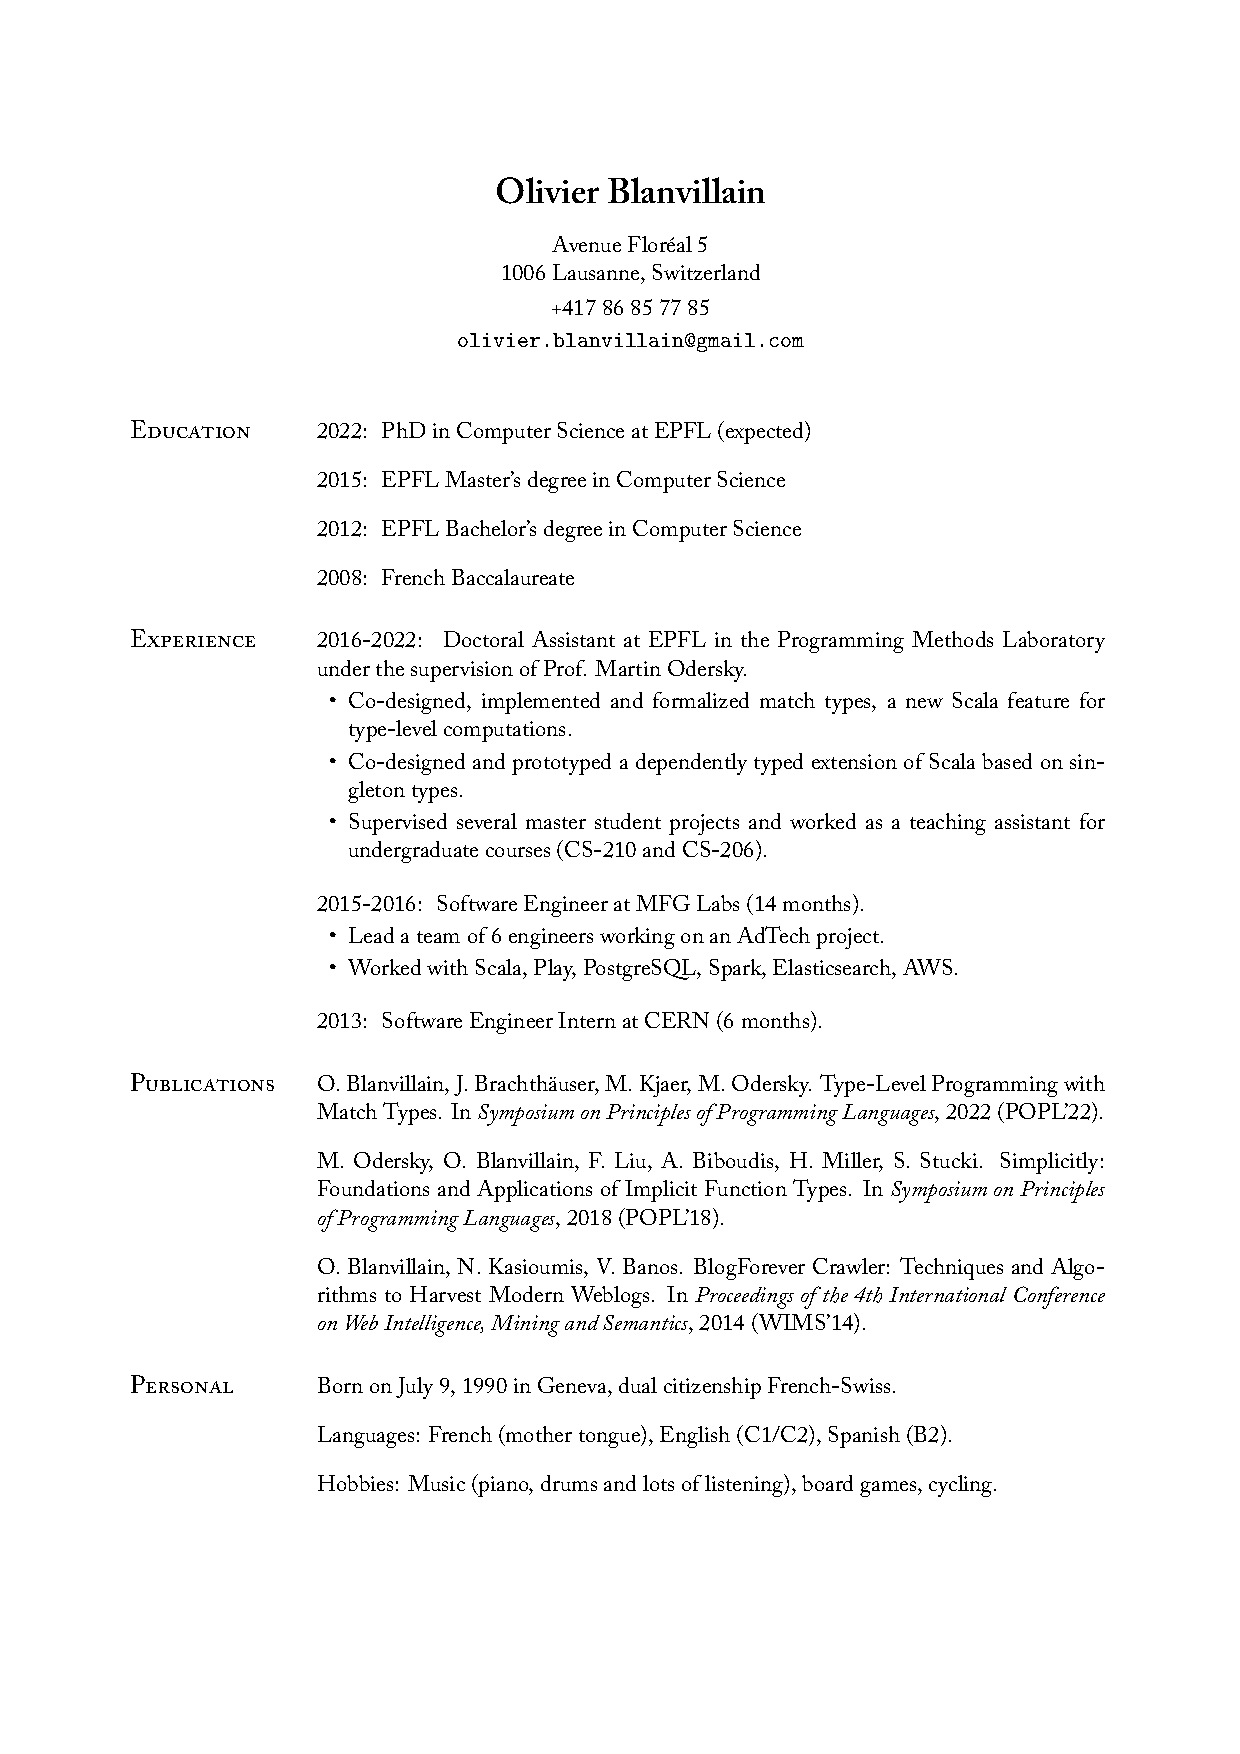
\includepdf{olivier-blanvillain-resume.pdf}
\thispagestyle{empty}~

\end{document}
